% !TeX spellcheck = en_US

to mechanically separate the ice layer from the sample holder, the adhesion needs to be reduced. Two different approaches are tested. First approach is using PDMS to lower adhesion. Additionally, in some cases the brittleness is used to additionally lower adhesion. To find favorable combinations of mixture ratio and plasma treatment at freezing at specific mixture ratios, tensile tests are conducted at room temperature first. With those results, tensile tests are conducted at cryogenic temperatures of complete samples with a thin ice layer. To further increase likelihood for separation, different factors influencing separation while using the finger are examined.

\section{PDMS experiments at room temperature}
%TODO: Vielleicht manches nach oben

To speed up the process of finding the right balance of PDMS Mixture ratio and plasma curing, experiments are done at room temperature. For this, a pulling machine is used. First the sample is prepared. Then, the sample is clamped to the pulling machine. Then a plexiglass stamp is aligned on top of the sample. With UV glue, the stamp is glued to the PDMS layer on the sample. Before gluing, The relative force and distance is set to zero on the pulling machine. After gluing, a couple minutes have to be waited, so no further stress changes are ongoing from the gluing process. After setting the force again to zero, the Machine is pulling on the sample with constant velocity. After detachment, the measurement is stopped. Afterwards, the stamp and the layer are analyzed under a microscope. The area of the attached UV glue to the sample is determined. With the maximum force and area, the maximum stress is calculated. Each experiment is repeated multiple times.


%\subsection{Plasma surface treatment of PDMS}

%TODO BOGEN SCHLIE?EN ZU STATE OF THE ART
Still, the effect of plasma activation under 50:1 is unknown. The plasma activation has two effects: first, it can increase the adhesion on ice to PDMS. second, the PDMS changes its structure, which could increase as well as decrease the strength of the PDMS layer. In the following, the effect of plasma activation on PDMS are examined. This is done at room temperature to speed up the process.

\subsection{Preparation of PDMS samples}

All PDMS samples are prepared in a similar way. The preparation starts with weighting out the desired amount of base coat and curing agent. The mixture is stirred intensively. The mixture is placed under a vacuum bell to gas out all air bubbles from stirring. Meanwhile the cover glass used as sample holders are cleaned with ethanol or isopropanol and dried. Afterwards, the PDMS mixture is spinned-coated onto the cover glass. Then the coated cover glasses are baked in the oven. The time and other variables needed for each process steps are dependent on the viscosity and the ratio of base to curing agent of the PDMS mixture (fig. \ref{table:preparationPDMSmixturereatios}). 

\begin{table}
	\centering
	\begin{tabular}{|c|c|c|c|}
		\hline
		 Preparation step & PDMS 1:2 & PDMS 4:1 & PDMS 50:1 \\
		\hline
		\hline
		Degassing in vacuum & \SI{30}{\minute} & \SI{30}{\minute} & \SI{1}{\hour}\\
		\hline
		Spin-coating & \SI{3000}{\rpm} for \SI{120}{\minute}  & \SI{3000}{\rpm} for \SI{120}{\minute} & \SI{3500}{\rpm} for \SI{150}{\minute} \\
		\hline
		Baking at \SI{80}{\degreeCelsius} & \SI{24}{\hour} & \SI{30}{\minute} & \SI{20}{\hour}\\
		\hline	
	\end{tabular}
	\caption{Differences in preparation of different mixture ratios of PDMS. The viscosity is increasing with higher base coat portion which results in longer degassing and spin-coating. Baking time takes longer with higher variation of the mixture ratio from the recommended 10:1 mixture ratio.}
	\label{table:preparationPDMSmixturereatios}
\end{table}

%For 1:2 base coat to curing agent weight ratio, the PDMS mixture is lightly viscious. A vacuum of \SI{30}{\minute} is drawn for degassing. A coat spinning time of \SI{120}{\minute} at \SI{3000}{\rpm} results in a smooth surface on all used slides. The baking time of at least \SI{24}{\hour} by \SI{80}{\degreeCelsius} is needed. 

For shorter baking times at 1:2 mixture ratio, plasma treatment has a slighlty different effect. Normally, touching a treated area will neutralize the effect of plasma treatment like hydrophility only locally on the touched surface. But here, touching the surface leads to the complete neutralization of plasma treatment when touching. In this work, the effect is undesired.

%For 4:1 base coat to curing agent weight ratio, the PDMS mixture is more viscious. The Vacuum and coat spinning are the same for \SI{30}{\minute} vacuum and \SI{3000}{\rpm} for \SI{120}{\minute}. But a baking time of \SI{30}{\minute} at \SI{80}{\degreeCelsius} is already sufficient to harden the PDMS. 

%For 50:1 base coat to curing agent weight ratio, the PDMS mixture is as viscious as the base coat. A longer vacuum of \SI{1}{\hour} is needed to air out all bubbles. The coat spinning speed and time is increased to \SI{3500}{\rpm} for \SI{180}{\minute} (NACHSCHAUEN). Also a longer baking time of \SI{20}{\hour} at \SI{80}{\degreeCelsius} is needed to harden the PDMS. 

In the coat spinning setup, each slide is coat spinned in succession of each other. With each spin-coating taking 2 to 3 minutes, this step takes up to multiple hours. To speed up the process, rectangular cover glass with \SI{20}{\milli\meter} x \SI{20}{\milli\meter} and \SI{24}{\milli\meter} x \SI{40}{\milli\meter} are coat spinned instead. afterwards the cover glass is split in multiple smaller pieces. 

The process is the same described as before for all PDMS mixture ratio, but with some minor adjustments. Before coat spinning, the glass is scratched with a diamond pencil. The scratches in the glass are weak points for breaking out smaller parts. Kapton tape is put over the scratched glass. The glass is put into the coat spinner with the taped side facing down. The PDMS is coat spinned onto the exposed glass side. The baking process is as previously described. After baking, the glass is broken into smaller pieces. This is done by dragging the attached tape over a table edge. Then the glass is fixed to the table with PDMS facing up. The PDMS is covered with Mylar foil to keep the PDMS clean. As the sticky side of the tape is not facing the table, the tape ends are additionally taped to the Table. Then smaller sample pieces can be broken off, The pieces are loosened from the tape by forcing a flat pincer between glass and the tape it is attached to.

This method has advantages as well as drawbacks to coat spinning small glass pieces separately. First, time is won by coat spinning, as one big glass can be split into several smaller ones. The Sample can stay fixed at the table without risking damaged. The samples can be broken off shortly before the experiment. But with hand scratching, only irregular and rectangular shapes can be won out of the bigger glass piece. also there is a significant loss of samples. This is by one part by breaking the sample. Some cracks do not follow the scratch, which leads to too small samples. Also in the process of loosening a piece cracks can form, making the piece too small for use.

In the end, both fabrication methods are used for different experiments. The small round cover glass is used in combination with the finger. The regular pieces are easier set up with the shuttle. The glass pieces broken out of a big cover glass are used with the pulling machine at room temperature. In this setup, fluctuations in size of the glass pieces are easier to handle and the clamping of the slide is more flexible. %TODO MAYBE was schreiben mit area dass es da weniger ausmacht oder so?

\subsection{Setup of the pulling machine}

To test the tensile strength of different PDMS mixtures and the effect of plasmacuring, the tensile testing machine inspekt table \SI{5}{\kilo\newton} manifactured by Hegewald \& Peschke is used. On the top part, two load cells are installed (Fig. \ref{fig:PullingMachineSetupBigPic}) The upper load cell is rated for \SI{5}{\kilo\newton}. the lower load cell is rated for up to \SI{100}{\newton}. As the upper load cell is extremely stiff and the forces are \SI{<<100}{\newton}, the upper load cell can be assumed as inflexible. On both the upper and lower part, two clamps are fixed onto the machine. On the bottom clamp a 3D-Printed stage is used for fixing on the sample.


%TODO SKIZZE
\begin{figure}[hbt!]
	\centering
	\begin{subfigure}[]{0.45\textwidth}
		\centering
		\begin{overpic}[width=6cm, height=9cm]{AufbauPullingMachine}
			\white
			\put(45, 82){\vector(-1,0){10}}
			\put(45, 82){\makebox(0,0)[bl]{\SI{5}{\kilo\newton}}}
			\put(45, 82){\makebox(0,0)[tl]{Load cell}}
			\put(20, 55){\vector(1,0){10}}
			\put(20, 55){\makebox(0,0)[br]{\SI{100}{\newton}}}
			\put(20, 55){\makebox(0,0)[tr]{Load cell}}
			\put(20, 35){\vector(1,0){10}}
			\put(20, 35){\makebox(0,0)[r]{top clamp}}
			\put(45, 20){\vector(-1,0){10}}
			\put(45, 20){\makebox(0,0)[bl]{bottom}}
			\put(45, 20){\makebox(0,0)[tl]{clamp}}
			%\put(21, 29){\vector(1,0){10}}
			%\put(21, 29){\makebox(0,0)[r]{Fig. \ref{fig:PullingMachineSetupZoomedPic}}}
		\end{overpic}
		\caption{}
		\label{fig:PullingMachineSetupBigPic}
	\end{subfigure}
	\begin{subfigure}[]{0.45\textwidth}
		\centering
		\begin{overpic}[width=6cm, height=9cm]{AufbauPullingMachineCloseup}
			\white
			\put(30, 78){\makebox(0,0)[c]{Top clamp}}	
			\put(30, 14){\makebox(0,0)[c]{Bottom clamp}}
			\put(21, 56){\vector(1,-1){10}}
			\put(21, 56){\makebox(0,0)[r]{Stamp}}
			\put(33, 26){\vector(0,1){10}}
			\put(33, 26){\makebox(0,0)[t]{Stage}}
			\put(45, 51){\vector(-1,-1){10}}
			\put(45, 51){\makebox(0,0)[l]{Brace}}
			\put(43, 39){\vector(-1,0){10}}
			\put(43, 39){\makebox(0,0)[l]{Screw}}
			\put(21.5, 40.5){\vector(1,0){10}}
			\put(21.5, 40.5){\makebox(0,0)[br]{UV glue}}
			\put(21.5, 40.5){\makebox(0,0)[tr]{on sample}}
			
		\end{overpic}
		\caption{}
		\label{fig:PullingMachineSetupZoomedPic}
	\end{subfigure}
	\caption{Setup for tensile tests of a thin PDMS layer. The Sample is placed on the stage. A brace is screwed over the sample to hold it in place. A stamp is fixed to the top clamp. The UV Glue is applied between stamp and sample and cured with 3 minutes UV Exposure. With the \SI{100}{\newton} load cell, the force is measured over distance pulled.}
	\label{fig:PullingMachineSetup}
\end{figure}

On the bottom, a 3D-Printed stage is clamped (Fig. \ref{fig:PullingMachineSetupZoomedPic}). The stage has four holes with threads for screws. Between the threads, the sample is placed. A brace similar to the "window" is fixed with screws onto the sample. A rectangle shape hole gives access for the UV-glue and the stamp. 

The Process of a pull test starts with clamping a new stamp on the top. Then the sample is plasma treated. After treatment, the sample is quickly transported to the pulling machine and fixed to the stage with screws. The stamp is aligned to the sample. When alignment is finished, the UV glue is given onto the stamp. the top is lowered on the sample. The UV glue is cured with UV radiation for \SI{3}{\minute}. After gluing, \SI{3}{\minute} are waited until forces settle resulting from curing and heat. Then, the pulling machine pulls with constant speed of \SI{0,01}{\milli\meter\per\second} and measures the stress strain curves. The process is ended manually. The now separated stamp and sample are stored for analyzation under a microscope. To calculate the maximum tensile stress, the area of the glue on the sample which is still attached to the stamp is measured.

%TODO BILDER VOM AUSMESSEN

\subsection{Tensile testing of PDMS}

In between experiments, small variations and improvements are done: two different stamps are used, one has an area of \SI{2}{\milli\meter} x \SI{3}{\milli\meter} and another stamp is \SI{3}{\milli\meter} x \SI{3}{\milli\meter}. Since the area is measured by the attached surface to the sample, the effect of a bigger stamp is taken into account. Also, in first experiments, while waiting of the stress changes to subside, the pulling machine is holding the position. As the UV glue cools and shrinks while being polymerized, the UV glue pulls the stamp and the surface more and more together. Before pulling, the machine is set back to zero. After pulling, an offset exists between before pulling which is set to zero and after pulling when both ends are disconnected. The offset is then corrected in evaluation. To avoid calculating an offset, the pulling machine sets the distance corresponding to the forces being constant to zero. The offset correction and new method increased the accuracy between pull tests.

To verify the setup, cover glass coated with 4:1 and 1:2 curing agent to base coat weight ratio and uncoated cover glass as control surface are compared. For each, multiple tensile tests are conducted. The Force over position is recorded and evaluated. Example results are shown in fig. \ref{fig:forceOverTime}. With the area measured of the UV-Glue residue on the stamp, The maximum tensile stress is calculated over successful tensile tests with mean and standard deviation.  

\begin{figure}[hbt!]
	\centering
	%% Creator: Matplotlib, PGF backend
%%
%% To include the figure in your LaTeX document, write
%%   \input{<filename>.pgf}
%%
%% Make sure the required packages are loaded in your preamble
%%   \usepackage{pgf}
%%
%% Also ensure that all the required font packages are loaded; for instance,
%% the lmodern package is sometimes necessary when using math font.
%%   \usepackage{lmodern}
%%
%% Figures using additional raster images can only be included by \input if
%% they are in the same directory as the main LaTeX file. For loading figures
%% from other directories you can use the `import` package
%%   \usepackage{import}
%%
%% and then include the figures with
%%   \import{<path to file>}{<filename>.pgf}
%%
%% Matplotlib used the following preamble
%%
\begingroup%
\makeatletter%
\begin{pgfpicture}%
\pgfpathrectangle{\pgfpointorigin}{\pgfqpoint{6.400000in}{4.800000in}}%
\pgfusepath{use as bounding box, clip}%
\begin{pgfscope}%
\pgfsetbuttcap%
\pgfsetmiterjoin%
\definecolor{currentfill}{rgb}{1.000000,1.000000,1.000000}%
\pgfsetfillcolor{currentfill}%
\pgfsetlinewidth{0.000000pt}%
\definecolor{currentstroke}{rgb}{1.000000,1.000000,1.000000}%
\pgfsetstrokecolor{currentstroke}%
\pgfsetdash{}{0pt}%
\pgfpathmoveto{\pgfqpoint{0.000000in}{0.000000in}}%
\pgfpathlineto{\pgfqpoint{6.400000in}{0.000000in}}%
\pgfpathlineto{\pgfqpoint{6.400000in}{4.800000in}}%
\pgfpathlineto{\pgfqpoint{0.000000in}{4.800000in}}%
\pgfpathlineto{\pgfqpoint{0.000000in}{0.000000in}}%
\pgfpathclose%
\pgfusepath{fill}%
\end{pgfscope}%
\begin{pgfscope}%
\pgfsetbuttcap%
\pgfsetmiterjoin%
\definecolor{currentfill}{rgb}{1.000000,1.000000,1.000000}%
\pgfsetfillcolor{currentfill}%
\pgfsetlinewidth{0.000000pt}%
\definecolor{currentstroke}{rgb}{0.000000,0.000000,0.000000}%
\pgfsetstrokecolor{currentstroke}%
\pgfsetstrokeopacity{0.000000}%
\pgfsetdash{}{0pt}%
\pgfpathmoveto{\pgfqpoint{0.800000in}{0.528000in}}%
\pgfpathlineto{\pgfqpoint{5.760000in}{0.528000in}}%
\pgfpathlineto{\pgfqpoint{5.760000in}{4.224000in}}%
\pgfpathlineto{\pgfqpoint{0.800000in}{4.224000in}}%
\pgfpathlineto{\pgfqpoint{0.800000in}{0.528000in}}%
\pgfpathclose%
\pgfusepath{fill}%
\end{pgfscope}%
\begin{pgfscope}%
\pgfpathrectangle{\pgfqpoint{0.800000in}{0.528000in}}{\pgfqpoint{4.960000in}{3.696000in}}%
\pgfusepath{clip}%
\pgfsetrectcap%
\pgfsetroundjoin%
\pgfsetlinewidth{0.803000pt}%
\definecolor{currentstroke}{rgb}{0.690196,0.690196,0.690196}%
\pgfsetstrokecolor{currentstroke}%
\pgfsetdash{}{0pt}%
\pgfpathmoveto{\pgfqpoint{1.025455in}{0.528000in}}%
\pgfpathlineto{\pgfqpoint{1.025455in}{4.224000in}}%
\pgfusepath{stroke}%
\end{pgfscope}%
\begin{pgfscope}%
\pgfsetbuttcap%
\pgfsetroundjoin%
\definecolor{currentfill}{rgb}{0.000000,0.000000,0.000000}%
\pgfsetfillcolor{currentfill}%
\pgfsetlinewidth{0.803000pt}%
\definecolor{currentstroke}{rgb}{0.000000,0.000000,0.000000}%
\pgfsetstrokecolor{currentstroke}%
\pgfsetdash{}{0pt}%
\pgfsys@defobject{currentmarker}{\pgfqpoint{0.000000in}{-0.048611in}}{\pgfqpoint{0.000000in}{0.000000in}}{%
\pgfpathmoveto{\pgfqpoint{0.000000in}{0.000000in}}%
\pgfpathlineto{\pgfqpoint{0.000000in}{-0.048611in}}%
\pgfusepath{stroke,fill}%
}%
\begin{pgfscope}%
\pgfsys@transformshift{1.025455in}{0.528000in}%
\pgfsys@useobject{currentmarker}{}%
\end{pgfscope}%
\end{pgfscope}%
\begin{pgfscope}%
\definecolor{textcolor}{rgb}{0.000000,0.000000,0.000000}%
\pgfsetstrokecolor{textcolor}%
\pgfsetfillcolor{textcolor}%
\pgftext[x=1.025455in,y=0.430778in,,top]{\color{textcolor}\rmfamily\fontsize{9.000000}{10.800000}\selectfont \(\displaystyle {0.0}\)}%
\end{pgfscope}%
\begin{pgfscope}%
\pgfpathrectangle{\pgfqpoint{0.800000in}{0.528000in}}{\pgfqpoint{4.960000in}{3.696000in}}%
\pgfusepath{clip}%
\pgfsetrectcap%
\pgfsetroundjoin%
\pgfsetlinewidth{0.803000pt}%
\definecolor{currentstroke}{rgb}{0.690196,0.690196,0.690196}%
\pgfsetstrokecolor{currentstroke}%
\pgfsetdash{}{0pt}%
\pgfpathmoveto{\pgfqpoint{1.852963in}{0.528000in}}%
\pgfpathlineto{\pgfqpoint{1.852963in}{4.224000in}}%
\pgfusepath{stroke}%
\end{pgfscope}%
\begin{pgfscope}%
\pgfsetbuttcap%
\pgfsetroundjoin%
\definecolor{currentfill}{rgb}{0.000000,0.000000,0.000000}%
\pgfsetfillcolor{currentfill}%
\pgfsetlinewidth{0.803000pt}%
\definecolor{currentstroke}{rgb}{0.000000,0.000000,0.000000}%
\pgfsetstrokecolor{currentstroke}%
\pgfsetdash{}{0pt}%
\pgfsys@defobject{currentmarker}{\pgfqpoint{0.000000in}{-0.048611in}}{\pgfqpoint{0.000000in}{0.000000in}}{%
\pgfpathmoveto{\pgfqpoint{0.000000in}{0.000000in}}%
\pgfpathlineto{\pgfqpoint{0.000000in}{-0.048611in}}%
\pgfusepath{stroke,fill}%
}%
\begin{pgfscope}%
\pgfsys@transformshift{1.852963in}{0.528000in}%
\pgfsys@useobject{currentmarker}{}%
\end{pgfscope}%
\end{pgfscope}%
\begin{pgfscope}%
\definecolor{textcolor}{rgb}{0.000000,0.000000,0.000000}%
\pgfsetstrokecolor{textcolor}%
\pgfsetfillcolor{textcolor}%
\pgftext[x=1.852963in,y=0.430778in,,top]{\color{textcolor}\rmfamily\fontsize{9.000000}{10.800000}\selectfont \(\displaystyle {0.1}\)}%
\end{pgfscope}%
\begin{pgfscope}%
\pgfpathrectangle{\pgfqpoint{0.800000in}{0.528000in}}{\pgfqpoint{4.960000in}{3.696000in}}%
\pgfusepath{clip}%
\pgfsetrectcap%
\pgfsetroundjoin%
\pgfsetlinewidth{0.803000pt}%
\definecolor{currentstroke}{rgb}{0.690196,0.690196,0.690196}%
\pgfsetstrokecolor{currentstroke}%
\pgfsetdash{}{0pt}%
\pgfpathmoveto{\pgfqpoint{2.680470in}{0.528000in}}%
\pgfpathlineto{\pgfqpoint{2.680470in}{4.224000in}}%
\pgfusepath{stroke}%
\end{pgfscope}%
\begin{pgfscope}%
\pgfsetbuttcap%
\pgfsetroundjoin%
\definecolor{currentfill}{rgb}{0.000000,0.000000,0.000000}%
\pgfsetfillcolor{currentfill}%
\pgfsetlinewidth{0.803000pt}%
\definecolor{currentstroke}{rgb}{0.000000,0.000000,0.000000}%
\pgfsetstrokecolor{currentstroke}%
\pgfsetdash{}{0pt}%
\pgfsys@defobject{currentmarker}{\pgfqpoint{0.000000in}{-0.048611in}}{\pgfqpoint{0.000000in}{0.000000in}}{%
\pgfpathmoveto{\pgfqpoint{0.000000in}{0.000000in}}%
\pgfpathlineto{\pgfqpoint{0.000000in}{-0.048611in}}%
\pgfusepath{stroke,fill}%
}%
\begin{pgfscope}%
\pgfsys@transformshift{2.680470in}{0.528000in}%
\pgfsys@useobject{currentmarker}{}%
\end{pgfscope}%
\end{pgfscope}%
\begin{pgfscope}%
\definecolor{textcolor}{rgb}{0.000000,0.000000,0.000000}%
\pgfsetstrokecolor{textcolor}%
\pgfsetfillcolor{textcolor}%
\pgftext[x=2.680470in,y=0.430778in,,top]{\color{textcolor}\rmfamily\fontsize{9.000000}{10.800000}\selectfont \(\displaystyle {0.2}\)}%
\end{pgfscope}%
\begin{pgfscope}%
\pgfpathrectangle{\pgfqpoint{0.800000in}{0.528000in}}{\pgfqpoint{4.960000in}{3.696000in}}%
\pgfusepath{clip}%
\pgfsetrectcap%
\pgfsetroundjoin%
\pgfsetlinewidth{0.803000pt}%
\definecolor{currentstroke}{rgb}{0.690196,0.690196,0.690196}%
\pgfsetstrokecolor{currentstroke}%
\pgfsetdash{}{0pt}%
\pgfpathmoveto{\pgfqpoint{3.507978in}{0.528000in}}%
\pgfpathlineto{\pgfqpoint{3.507978in}{4.224000in}}%
\pgfusepath{stroke}%
\end{pgfscope}%
\begin{pgfscope}%
\pgfsetbuttcap%
\pgfsetroundjoin%
\definecolor{currentfill}{rgb}{0.000000,0.000000,0.000000}%
\pgfsetfillcolor{currentfill}%
\pgfsetlinewidth{0.803000pt}%
\definecolor{currentstroke}{rgb}{0.000000,0.000000,0.000000}%
\pgfsetstrokecolor{currentstroke}%
\pgfsetdash{}{0pt}%
\pgfsys@defobject{currentmarker}{\pgfqpoint{0.000000in}{-0.048611in}}{\pgfqpoint{0.000000in}{0.000000in}}{%
\pgfpathmoveto{\pgfqpoint{0.000000in}{0.000000in}}%
\pgfpathlineto{\pgfqpoint{0.000000in}{-0.048611in}}%
\pgfusepath{stroke,fill}%
}%
\begin{pgfscope}%
\pgfsys@transformshift{3.507978in}{0.528000in}%
\pgfsys@useobject{currentmarker}{}%
\end{pgfscope}%
\end{pgfscope}%
\begin{pgfscope}%
\definecolor{textcolor}{rgb}{0.000000,0.000000,0.000000}%
\pgfsetstrokecolor{textcolor}%
\pgfsetfillcolor{textcolor}%
\pgftext[x=3.507978in,y=0.430778in,,top]{\color{textcolor}\rmfamily\fontsize{9.000000}{10.800000}\selectfont \(\displaystyle {0.3}\)}%
\end{pgfscope}%
\begin{pgfscope}%
\pgfpathrectangle{\pgfqpoint{0.800000in}{0.528000in}}{\pgfqpoint{4.960000in}{3.696000in}}%
\pgfusepath{clip}%
\pgfsetrectcap%
\pgfsetroundjoin%
\pgfsetlinewidth{0.803000pt}%
\definecolor{currentstroke}{rgb}{0.690196,0.690196,0.690196}%
\pgfsetstrokecolor{currentstroke}%
\pgfsetdash{}{0pt}%
\pgfpathmoveto{\pgfqpoint{4.335486in}{0.528000in}}%
\pgfpathlineto{\pgfqpoint{4.335486in}{4.224000in}}%
\pgfusepath{stroke}%
\end{pgfscope}%
\begin{pgfscope}%
\pgfsetbuttcap%
\pgfsetroundjoin%
\definecolor{currentfill}{rgb}{0.000000,0.000000,0.000000}%
\pgfsetfillcolor{currentfill}%
\pgfsetlinewidth{0.803000pt}%
\definecolor{currentstroke}{rgb}{0.000000,0.000000,0.000000}%
\pgfsetstrokecolor{currentstroke}%
\pgfsetdash{}{0pt}%
\pgfsys@defobject{currentmarker}{\pgfqpoint{0.000000in}{-0.048611in}}{\pgfqpoint{0.000000in}{0.000000in}}{%
\pgfpathmoveto{\pgfqpoint{0.000000in}{0.000000in}}%
\pgfpathlineto{\pgfqpoint{0.000000in}{-0.048611in}}%
\pgfusepath{stroke,fill}%
}%
\begin{pgfscope}%
\pgfsys@transformshift{4.335486in}{0.528000in}%
\pgfsys@useobject{currentmarker}{}%
\end{pgfscope}%
\end{pgfscope}%
\begin{pgfscope}%
\definecolor{textcolor}{rgb}{0.000000,0.000000,0.000000}%
\pgfsetstrokecolor{textcolor}%
\pgfsetfillcolor{textcolor}%
\pgftext[x=4.335486in,y=0.430778in,,top]{\color{textcolor}\rmfamily\fontsize{9.000000}{10.800000}\selectfont \(\displaystyle {0.4}\)}%
\end{pgfscope}%
\begin{pgfscope}%
\pgfpathrectangle{\pgfqpoint{0.800000in}{0.528000in}}{\pgfqpoint{4.960000in}{3.696000in}}%
\pgfusepath{clip}%
\pgfsetrectcap%
\pgfsetroundjoin%
\pgfsetlinewidth{0.803000pt}%
\definecolor{currentstroke}{rgb}{0.690196,0.690196,0.690196}%
\pgfsetstrokecolor{currentstroke}%
\pgfsetdash{}{0pt}%
\pgfpathmoveto{\pgfqpoint{5.162994in}{0.528000in}}%
\pgfpathlineto{\pgfqpoint{5.162994in}{4.224000in}}%
\pgfusepath{stroke}%
\end{pgfscope}%
\begin{pgfscope}%
\pgfsetbuttcap%
\pgfsetroundjoin%
\definecolor{currentfill}{rgb}{0.000000,0.000000,0.000000}%
\pgfsetfillcolor{currentfill}%
\pgfsetlinewidth{0.803000pt}%
\definecolor{currentstroke}{rgb}{0.000000,0.000000,0.000000}%
\pgfsetstrokecolor{currentstroke}%
\pgfsetdash{}{0pt}%
\pgfsys@defobject{currentmarker}{\pgfqpoint{0.000000in}{-0.048611in}}{\pgfqpoint{0.000000in}{0.000000in}}{%
\pgfpathmoveto{\pgfqpoint{0.000000in}{0.000000in}}%
\pgfpathlineto{\pgfqpoint{0.000000in}{-0.048611in}}%
\pgfusepath{stroke,fill}%
}%
\begin{pgfscope}%
\pgfsys@transformshift{5.162994in}{0.528000in}%
\pgfsys@useobject{currentmarker}{}%
\end{pgfscope}%
\end{pgfscope}%
\begin{pgfscope}%
\definecolor{textcolor}{rgb}{0.000000,0.000000,0.000000}%
\pgfsetstrokecolor{textcolor}%
\pgfsetfillcolor{textcolor}%
\pgftext[x=5.162994in,y=0.430778in,,top]{\color{textcolor}\rmfamily\fontsize{9.000000}{10.800000}\selectfont \(\displaystyle {0.5}\)}%
\end{pgfscope}%
\begin{pgfscope}%
\definecolor{textcolor}{rgb}{0.000000,0.000000,0.000000}%
\pgfsetstrokecolor{textcolor}%
\pgfsetfillcolor{textcolor}%
\pgftext[x=3.280000in,y=0.264111in,,top]{\color{textcolor}\rmfamily\fontsize{10.000000}{12.000000}\selectfont Displacement in mm}%
\end{pgfscope}%
\begin{pgfscope}%
\pgfpathrectangle{\pgfqpoint{0.800000in}{0.528000in}}{\pgfqpoint{4.960000in}{3.696000in}}%
\pgfusepath{clip}%
\pgfsetrectcap%
\pgfsetroundjoin%
\pgfsetlinewidth{0.803000pt}%
\definecolor{currentstroke}{rgb}{0.690196,0.690196,0.690196}%
\pgfsetstrokecolor{currentstroke}%
\pgfsetdash{}{0pt}%
\pgfpathmoveto{\pgfqpoint{0.800000in}{0.842955in}}%
\pgfpathlineto{\pgfqpoint{5.760000in}{0.842955in}}%
\pgfusepath{stroke}%
\end{pgfscope}%
\begin{pgfscope}%
\pgfsetbuttcap%
\pgfsetroundjoin%
\definecolor{currentfill}{rgb}{0.000000,0.000000,0.000000}%
\pgfsetfillcolor{currentfill}%
\pgfsetlinewidth{0.803000pt}%
\definecolor{currentstroke}{rgb}{0.000000,0.000000,0.000000}%
\pgfsetstrokecolor{currentstroke}%
\pgfsetdash{}{0pt}%
\pgfsys@defobject{currentmarker}{\pgfqpoint{-0.048611in}{0.000000in}}{\pgfqpoint{-0.000000in}{0.000000in}}{%
\pgfpathmoveto{\pgfqpoint{-0.000000in}{0.000000in}}%
\pgfpathlineto{\pgfqpoint{-0.048611in}{0.000000in}}%
\pgfusepath{stroke,fill}%
}%
\begin{pgfscope}%
\pgfsys@transformshift{0.800000in}{0.842955in}%
\pgfsys@useobject{currentmarker}{}%
\end{pgfscope}%
\end{pgfscope}%
\begin{pgfscope}%
\definecolor{textcolor}{rgb}{0.000000,0.000000,0.000000}%
\pgfsetstrokecolor{textcolor}%
\pgfsetfillcolor{textcolor}%
\pgftext[x=0.633333in, y=0.794730in, left, base]{\color{textcolor}\rmfamily\fontsize{10.000000}{12.000000}\selectfont \(\displaystyle {0}\)}%
\end{pgfscope}%
\begin{pgfscope}%
\pgfpathrectangle{\pgfqpoint{0.800000in}{0.528000in}}{\pgfqpoint{4.960000in}{3.696000in}}%
\pgfusepath{clip}%
\pgfsetrectcap%
\pgfsetroundjoin%
\pgfsetlinewidth{0.803000pt}%
\definecolor{currentstroke}{rgb}{0.690196,0.690196,0.690196}%
\pgfsetstrokecolor{currentstroke}%
\pgfsetdash{}{0pt}%
\pgfpathmoveto{\pgfqpoint{0.800000in}{1.283732in}}%
\pgfpathlineto{\pgfqpoint{5.760000in}{1.283732in}}%
\pgfusepath{stroke}%
\end{pgfscope}%
\begin{pgfscope}%
\pgfsetbuttcap%
\pgfsetroundjoin%
\definecolor{currentfill}{rgb}{0.000000,0.000000,0.000000}%
\pgfsetfillcolor{currentfill}%
\pgfsetlinewidth{0.803000pt}%
\definecolor{currentstroke}{rgb}{0.000000,0.000000,0.000000}%
\pgfsetstrokecolor{currentstroke}%
\pgfsetdash{}{0pt}%
\pgfsys@defobject{currentmarker}{\pgfqpoint{-0.048611in}{0.000000in}}{\pgfqpoint{-0.000000in}{0.000000in}}{%
\pgfpathmoveto{\pgfqpoint{-0.000000in}{0.000000in}}%
\pgfpathlineto{\pgfqpoint{-0.048611in}{0.000000in}}%
\pgfusepath{stroke,fill}%
}%
\begin{pgfscope}%
\pgfsys@transformshift{0.800000in}{1.283732in}%
\pgfsys@useobject{currentmarker}{}%
\end{pgfscope}%
\end{pgfscope}%
\begin{pgfscope}%
\definecolor{textcolor}{rgb}{0.000000,0.000000,0.000000}%
\pgfsetstrokecolor{textcolor}%
\pgfsetfillcolor{textcolor}%
\pgftext[x=0.633333in, y=1.235507in, left, base]{\color{textcolor}\rmfamily\fontsize{10.000000}{12.000000}\selectfont \(\displaystyle {2}\)}%
\end{pgfscope}%
\begin{pgfscope}%
\pgfpathrectangle{\pgfqpoint{0.800000in}{0.528000in}}{\pgfqpoint{4.960000in}{3.696000in}}%
\pgfusepath{clip}%
\pgfsetrectcap%
\pgfsetroundjoin%
\pgfsetlinewidth{0.803000pt}%
\definecolor{currentstroke}{rgb}{0.690196,0.690196,0.690196}%
\pgfsetstrokecolor{currentstroke}%
\pgfsetdash{}{0pt}%
\pgfpathmoveto{\pgfqpoint{0.800000in}{1.724509in}}%
\pgfpathlineto{\pgfqpoint{5.760000in}{1.724509in}}%
\pgfusepath{stroke}%
\end{pgfscope}%
\begin{pgfscope}%
\pgfsetbuttcap%
\pgfsetroundjoin%
\definecolor{currentfill}{rgb}{0.000000,0.000000,0.000000}%
\pgfsetfillcolor{currentfill}%
\pgfsetlinewidth{0.803000pt}%
\definecolor{currentstroke}{rgb}{0.000000,0.000000,0.000000}%
\pgfsetstrokecolor{currentstroke}%
\pgfsetdash{}{0pt}%
\pgfsys@defobject{currentmarker}{\pgfqpoint{-0.048611in}{0.000000in}}{\pgfqpoint{-0.000000in}{0.000000in}}{%
\pgfpathmoveto{\pgfqpoint{-0.000000in}{0.000000in}}%
\pgfpathlineto{\pgfqpoint{-0.048611in}{0.000000in}}%
\pgfusepath{stroke,fill}%
}%
\begin{pgfscope}%
\pgfsys@transformshift{0.800000in}{1.724509in}%
\pgfsys@useobject{currentmarker}{}%
\end{pgfscope}%
\end{pgfscope}%
\begin{pgfscope}%
\definecolor{textcolor}{rgb}{0.000000,0.000000,0.000000}%
\pgfsetstrokecolor{textcolor}%
\pgfsetfillcolor{textcolor}%
\pgftext[x=0.633333in, y=1.676284in, left, base]{\color{textcolor}\rmfamily\fontsize{10.000000}{12.000000}\selectfont \(\displaystyle {4}\)}%
\end{pgfscope}%
\begin{pgfscope}%
\pgfpathrectangle{\pgfqpoint{0.800000in}{0.528000in}}{\pgfqpoint{4.960000in}{3.696000in}}%
\pgfusepath{clip}%
\pgfsetrectcap%
\pgfsetroundjoin%
\pgfsetlinewidth{0.803000pt}%
\definecolor{currentstroke}{rgb}{0.690196,0.690196,0.690196}%
\pgfsetstrokecolor{currentstroke}%
\pgfsetdash{}{0pt}%
\pgfpathmoveto{\pgfqpoint{0.800000in}{2.165286in}}%
\pgfpathlineto{\pgfqpoint{5.760000in}{2.165286in}}%
\pgfusepath{stroke}%
\end{pgfscope}%
\begin{pgfscope}%
\pgfsetbuttcap%
\pgfsetroundjoin%
\definecolor{currentfill}{rgb}{0.000000,0.000000,0.000000}%
\pgfsetfillcolor{currentfill}%
\pgfsetlinewidth{0.803000pt}%
\definecolor{currentstroke}{rgb}{0.000000,0.000000,0.000000}%
\pgfsetstrokecolor{currentstroke}%
\pgfsetdash{}{0pt}%
\pgfsys@defobject{currentmarker}{\pgfqpoint{-0.048611in}{0.000000in}}{\pgfqpoint{-0.000000in}{0.000000in}}{%
\pgfpathmoveto{\pgfqpoint{-0.000000in}{0.000000in}}%
\pgfpathlineto{\pgfqpoint{-0.048611in}{0.000000in}}%
\pgfusepath{stroke,fill}%
}%
\begin{pgfscope}%
\pgfsys@transformshift{0.800000in}{2.165286in}%
\pgfsys@useobject{currentmarker}{}%
\end{pgfscope}%
\end{pgfscope}%
\begin{pgfscope}%
\definecolor{textcolor}{rgb}{0.000000,0.000000,0.000000}%
\pgfsetstrokecolor{textcolor}%
\pgfsetfillcolor{textcolor}%
\pgftext[x=0.633333in, y=2.117061in, left, base]{\color{textcolor}\rmfamily\fontsize{10.000000}{12.000000}\selectfont \(\displaystyle {6}\)}%
\end{pgfscope}%
\begin{pgfscope}%
\pgfpathrectangle{\pgfqpoint{0.800000in}{0.528000in}}{\pgfqpoint{4.960000in}{3.696000in}}%
\pgfusepath{clip}%
\pgfsetrectcap%
\pgfsetroundjoin%
\pgfsetlinewidth{0.803000pt}%
\definecolor{currentstroke}{rgb}{0.690196,0.690196,0.690196}%
\pgfsetstrokecolor{currentstroke}%
\pgfsetdash{}{0pt}%
\pgfpathmoveto{\pgfqpoint{0.800000in}{2.606064in}}%
\pgfpathlineto{\pgfqpoint{5.760000in}{2.606064in}}%
\pgfusepath{stroke}%
\end{pgfscope}%
\begin{pgfscope}%
\pgfsetbuttcap%
\pgfsetroundjoin%
\definecolor{currentfill}{rgb}{0.000000,0.000000,0.000000}%
\pgfsetfillcolor{currentfill}%
\pgfsetlinewidth{0.803000pt}%
\definecolor{currentstroke}{rgb}{0.000000,0.000000,0.000000}%
\pgfsetstrokecolor{currentstroke}%
\pgfsetdash{}{0pt}%
\pgfsys@defobject{currentmarker}{\pgfqpoint{-0.048611in}{0.000000in}}{\pgfqpoint{-0.000000in}{0.000000in}}{%
\pgfpathmoveto{\pgfqpoint{-0.000000in}{0.000000in}}%
\pgfpathlineto{\pgfqpoint{-0.048611in}{0.000000in}}%
\pgfusepath{stroke,fill}%
}%
\begin{pgfscope}%
\pgfsys@transformshift{0.800000in}{2.606064in}%
\pgfsys@useobject{currentmarker}{}%
\end{pgfscope}%
\end{pgfscope}%
\begin{pgfscope}%
\definecolor{textcolor}{rgb}{0.000000,0.000000,0.000000}%
\pgfsetstrokecolor{textcolor}%
\pgfsetfillcolor{textcolor}%
\pgftext[x=0.633333in, y=2.557838in, left, base]{\color{textcolor}\rmfamily\fontsize{10.000000}{12.000000}\selectfont \(\displaystyle {8}\)}%
\end{pgfscope}%
\begin{pgfscope}%
\pgfpathrectangle{\pgfqpoint{0.800000in}{0.528000in}}{\pgfqpoint{4.960000in}{3.696000in}}%
\pgfusepath{clip}%
\pgfsetrectcap%
\pgfsetroundjoin%
\pgfsetlinewidth{0.803000pt}%
\definecolor{currentstroke}{rgb}{0.690196,0.690196,0.690196}%
\pgfsetstrokecolor{currentstroke}%
\pgfsetdash{}{0pt}%
\pgfpathmoveto{\pgfqpoint{0.800000in}{3.046841in}}%
\pgfpathlineto{\pgfqpoint{5.760000in}{3.046841in}}%
\pgfusepath{stroke}%
\end{pgfscope}%
\begin{pgfscope}%
\pgfsetbuttcap%
\pgfsetroundjoin%
\definecolor{currentfill}{rgb}{0.000000,0.000000,0.000000}%
\pgfsetfillcolor{currentfill}%
\pgfsetlinewidth{0.803000pt}%
\definecolor{currentstroke}{rgb}{0.000000,0.000000,0.000000}%
\pgfsetstrokecolor{currentstroke}%
\pgfsetdash{}{0pt}%
\pgfsys@defobject{currentmarker}{\pgfqpoint{-0.048611in}{0.000000in}}{\pgfqpoint{-0.000000in}{0.000000in}}{%
\pgfpathmoveto{\pgfqpoint{-0.000000in}{0.000000in}}%
\pgfpathlineto{\pgfqpoint{-0.048611in}{0.000000in}}%
\pgfusepath{stroke,fill}%
}%
\begin{pgfscope}%
\pgfsys@transformshift{0.800000in}{3.046841in}%
\pgfsys@useobject{currentmarker}{}%
\end{pgfscope}%
\end{pgfscope}%
\begin{pgfscope}%
\definecolor{textcolor}{rgb}{0.000000,0.000000,0.000000}%
\pgfsetstrokecolor{textcolor}%
\pgfsetfillcolor{textcolor}%
\pgftext[x=0.563888in, y=2.998615in, left, base]{\color{textcolor}\rmfamily\fontsize{10.000000}{12.000000}\selectfont \(\displaystyle {10}\)}%
\end{pgfscope}%
\begin{pgfscope}%
\pgfpathrectangle{\pgfqpoint{0.800000in}{0.528000in}}{\pgfqpoint{4.960000in}{3.696000in}}%
\pgfusepath{clip}%
\pgfsetrectcap%
\pgfsetroundjoin%
\pgfsetlinewidth{0.803000pt}%
\definecolor{currentstroke}{rgb}{0.690196,0.690196,0.690196}%
\pgfsetstrokecolor{currentstroke}%
\pgfsetdash{}{0pt}%
\pgfpathmoveto{\pgfqpoint{0.800000in}{3.487618in}}%
\pgfpathlineto{\pgfqpoint{5.760000in}{3.487618in}}%
\pgfusepath{stroke}%
\end{pgfscope}%
\begin{pgfscope}%
\pgfsetbuttcap%
\pgfsetroundjoin%
\definecolor{currentfill}{rgb}{0.000000,0.000000,0.000000}%
\pgfsetfillcolor{currentfill}%
\pgfsetlinewidth{0.803000pt}%
\definecolor{currentstroke}{rgb}{0.000000,0.000000,0.000000}%
\pgfsetstrokecolor{currentstroke}%
\pgfsetdash{}{0pt}%
\pgfsys@defobject{currentmarker}{\pgfqpoint{-0.048611in}{0.000000in}}{\pgfqpoint{-0.000000in}{0.000000in}}{%
\pgfpathmoveto{\pgfqpoint{-0.000000in}{0.000000in}}%
\pgfpathlineto{\pgfqpoint{-0.048611in}{0.000000in}}%
\pgfusepath{stroke,fill}%
}%
\begin{pgfscope}%
\pgfsys@transformshift{0.800000in}{3.487618in}%
\pgfsys@useobject{currentmarker}{}%
\end{pgfscope}%
\end{pgfscope}%
\begin{pgfscope}%
\definecolor{textcolor}{rgb}{0.000000,0.000000,0.000000}%
\pgfsetstrokecolor{textcolor}%
\pgfsetfillcolor{textcolor}%
\pgftext[x=0.563888in, y=3.439393in, left, base]{\color{textcolor}\rmfamily\fontsize{10.000000}{12.000000}\selectfont \(\displaystyle {12}\)}%
\end{pgfscope}%
\begin{pgfscope}%
\pgfpathrectangle{\pgfqpoint{0.800000in}{0.528000in}}{\pgfqpoint{4.960000in}{3.696000in}}%
\pgfusepath{clip}%
\pgfsetrectcap%
\pgfsetroundjoin%
\pgfsetlinewidth{0.803000pt}%
\definecolor{currentstroke}{rgb}{0.690196,0.690196,0.690196}%
\pgfsetstrokecolor{currentstroke}%
\pgfsetdash{}{0pt}%
\pgfpathmoveto{\pgfqpoint{0.800000in}{3.928395in}}%
\pgfpathlineto{\pgfqpoint{5.760000in}{3.928395in}}%
\pgfusepath{stroke}%
\end{pgfscope}%
\begin{pgfscope}%
\pgfsetbuttcap%
\pgfsetroundjoin%
\definecolor{currentfill}{rgb}{0.000000,0.000000,0.000000}%
\pgfsetfillcolor{currentfill}%
\pgfsetlinewidth{0.803000pt}%
\definecolor{currentstroke}{rgb}{0.000000,0.000000,0.000000}%
\pgfsetstrokecolor{currentstroke}%
\pgfsetdash{}{0pt}%
\pgfsys@defobject{currentmarker}{\pgfqpoint{-0.048611in}{0.000000in}}{\pgfqpoint{-0.000000in}{0.000000in}}{%
\pgfpathmoveto{\pgfqpoint{-0.000000in}{0.000000in}}%
\pgfpathlineto{\pgfqpoint{-0.048611in}{0.000000in}}%
\pgfusepath{stroke,fill}%
}%
\begin{pgfscope}%
\pgfsys@transformshift{0.800000in}{3.928395in}%
\pgfsys@useobject{currentmarker}{}%
\end{pgfscope}%
\end{pgfscope}%
\begin{pgfscope}%
\definecolor{textcolor}{rgb}{0.000000,0.000000,0.000000}%
\pgfsetstrokecolor{textcolor}%
\pgfsetfillcolor{textcolor}%
\pgftext[x=0.563888in, y=3.880170in, left, base]{\color{textcolor}\rmfamily\fontsize{10.000000}{12.000000}\selectfont \(\displaystyle {14}\)}%
\end{pgfscope}%
\begin{pgfscope}%
\definecolor{textcolor}{rgb}{0.000000,0.000000,0.000000}%
\pgfsetstrokecolor{textcolor}%
\pgfsetfillcolor{textcolor}%
\pgftext[x=0.508333in,y=2.376000in,,bottom,rotate=90.000000]{\color{textcolor}\rmfamily\fontsize{10.000000}{12.000000}\selectfont Force in N}%
\end{pgfscope}%
\begin{pgfscope}%
\pgfpathrectangle{\pgfqpoint{0.800000in}{0.528000in}}{\pgfqpoint{4.960000in}{3.696000in}}%
\pgfusepath{clip}%
\pgfsetrectcap%
\pgfsetroundjoin%
\pgfsetlinewidth{1.505625pt}%
\definecolor{currentstroke}{rgb}{0.121569,0.466667,0.705882}%
\pgfsetstrokecolor{currentstroke}%
\pgfsetdash{}{0pt}%
\pgfpathmoveto{\pgfqpoint{1.025455in}{0.843418in}}%
\pgfpathlineto{\pgfqpoint{1.025595in}{0.842911in}}%
\pgfpathlineto{\pgfqpoint{1.026439in}{0.844167in}}%
\pgfpathlineto{\pgfqpoint{1.027490in}{0.844167in}}%
\pgfpathlineto{\pgfqpoint{1.029592in}{0.845688in}}%
\pgfpathlineto{\pgfqpoint{1.050991in}{0.865920in}}%
\pgfpathlineto{\pgfqpoint{1.055758in}{0.870966in}}%
\pgfpathlineto{\pgfqpoint{1.058778in}{0.873501in}}%
\pgfpathlineto{\pgfqpoint{1.093567in}{0.900036in}}%
\pgfpathlineto{\pgfqpoint{1.100725in}{0.905612in}}%
\pgfpathlineto{\pgfqpoint{1.102405in}{0.906361in}}%
\pgfpathlineto{\pgfqpoint{1.104159in}{0.907617in}}%
\pgfpathlineto{\pgfqpoint{1.107386in}{0.910152in}}%
\pgfpathlineto{\pgfqpoint{1.109000in}{0.911165in}}%
\pgfpathlineto{\pgfqpoint{1.113915in}{0.915463in}}%
\pgfpathlineto{\pgfqpoint{1.114825in}{0.915463in}}%
\pgfpathlineto{\pgfqpoint{1.117349in}{0.917997in}}%
\pgfpathlineto{\pgfqpoint{1.119948in}{0.919761in}}%
\pgfpathlineto{\pgfqpoint{1.123382in}{0.922802in}}%
\pgfpathlineto{\pgfqpoint{1.129836in}{0.927584in}}%
\pgfpathlineto{\pgfqpoint{1.134115in}{0.931397in}}%
\pgfpathlineto{\pgfqpoint{1.135728in}{0.932389in}}%
\pgfpathlineto{\pgfqpoint{1.141554in}{0.936686in}}%
\pgfpathlineto{\pgfqpoint{1.145758in}{0.940235in}}%
\pgfpathlineto{\pgfqpoint{1.147305in}{0.941491in}}%
\pgfpathlineto{\pgfqpoint{1.155862in}{0.947574in}}%
\pgfpathlineto{\pgfqpoint{1.159792in}{0.947309in}}%
\pgfpathlineto{\pgfqpoint{1.161613in}{0.942505in}}%
\pgfpathlineto{\pgfqpoint{1.162382in}{0.935937in}}%
\pgfpathlineto{\pgfqpoint{1.165750in}{0.820916in}}%
\pgfpathlineto{\pgfqpoint{1.168208in}{0.820674in}}%
\pgfpathlineto{\pgfqpoint{1.173190in}{0.819902in}}%
\pgfpathlineto{\pgfqpoint{1.176483in}{0.811814in}}%
\pgfpathlineto{\pgfqpoint{1.177253in}{0.811065in}}%
\pgfpathlineto{\pgfqpoint{1.178097in}{0.812079in}}%
\pgfpathlineto{\pgfqpoint{1.179785in}{0.811572in}}%
\pgfpathlineto{\pgfqpoint{1.270976in}{0.810800in}}%
\pgfpathlineto{\pgfqpoint{1.271820in}{0.810316in}}%
\pgfpathlineto{\pgfqpoint{1.272656in}{0.811307in}}%
\pgfpathlineto{\pgfqpoint{1.273434in}{0.810558in}}%
\pgfpathlineto{\pgfqpoint{1.280021in}{0.811307in}}%
\pgfpathlineto{\pgfqpoint{1.281634in}{0.811307in}}%
\pgfpathlineto{\pgfqpoint{1.423130in}{0.811065in}}%
\pgfpathlineto{\pgfqpoint{1.424040in}{0.809809in}}%
\pgfpathlineto{\pgfqpoint{1.425654in}{0.812321in}}%
\pgfpathlineto{\pgfqpoint{1.427268in}{0.809544in}}%
\pgfpathlineto{\pgfqpoint{1.429022in}{0.811307in}}%
\pgfpathlineto{\pgfqpoint{1.430702in}{0.810800in}}%
\pgfpathlineto{\pgfqpoint{1.431471in}{0.810316in}}%
\pgfpathlineto{\pgfqpoint{1.432249in}{0.811307in}}%
\pgfpathlineto{\pgfqpoint{1.433929in}{0.810800in}}%
\pgfpathlineto{\pgfqpoint{1.434773in}{0.810558in}}%
\pgfpathlineto{\pgfqpoint{1.436453in}{0.811065in}}%
\pgfpathlineto{\pgfqpoint{1.439680in}{0.810800in}}%
\pgfpathlineto{\pgfqpoint{1.671738in}{0.811065in}}%
\pgfpathlineto{\pgfqpoint{1.672508in}{0.809037in}}%
\pgfpathlineto{\pgfqpoint{1.673352in}{0.815362in}}%
\pgfpathlineto{\pgfqpoint{1.674328in}{0.807274in}}%
\pgfpathlineto{\pgfqpoint{1.675098in}{0.811307in}}%
\pgfpathlineto{\pgfqpoint{1.676016in}{0.809809in}}%
\pgfpathlineto{\pgfqpoint{1.676786in}{0.812586in}}%
\pgfpathlineto{\pgfqpoint{1.677630in}{0.810051in}}%
\pgfpathlineto{\pgfqpoint{1.678466in}{0.810558in}}%
\pgfpathlineto{\pgfqpoint{1.679384in}{0.812321in}}%
\pgfpathlineto{\pgfqpoint{1.680154in}{0.808288in}}%
\pgfpathlineto{\pgfqpoint{1.680924in}{0.812828in}}%
\pgfpathlineto{\pgfqpoint{1.681768in}{0.808530in}}%
\pgfpathlineto{\pgfqpoint{1.682537in}{0.812586in}}%
\pgfpathlineto{\pgfqpoint{1.683381in}{0.809302in}}%
\pgfpathlineto{\pgfqpoint{1.684217in}{0.811572in}}%
\pgfpathlineto{\pgfqpoint{1.684995in}{0.809809in}}%
\pgfpathlineto{\pgfqpoint{1.685698in}{0.811814in}}%
\pgfpathlineto{\pgfqpoint{1.687444in}{0.810558in}}%
\pgfpathlineto{\pgfqpoint{1.692145in}{0.810316in}}%
\pgfpathlineto{\pgfqpoint{1.692922in}{0.812079in}}%
\pgfpathlineto{\pgfqpoint{1.693692in}{0.809302in}}%
\pgfpathlineto{\pgfqpoint{1.694536in}{0.812079in}}%
\pgfpathlineto{\pgfqpoint{1.695306in}{0.811065in}}%
\pgfpathlineto{\pgfqpoint{1.696150in}{0.810051in}}%
\pgfpathlineto{\pgfqpoint{1.697830in}{0.811307in}}%
\pgfpathlineto{\pgfqpoint{1.698533in}{0.809809in}}%
\pgfpathlineto{\pgfqpoint{1.699518in}{0.810316in}}%
\pgfpathlineto{\pgfqpoint{1.700353in}{0.811572in}}%
\pgfpathlineto{\pgfqpoint{1.701198in}{0.810051in}}%
\pgfpathlineto{\pgfqpoint{1.702811in}{0.810800in}}%
\pgfpathlineto{\pgfqpoint{1.704566in}{0.811065in}}%
\pgfpathlineto{\pgfqpoint{1.710524in}{0.811065in}}%
\pgfpathlineto{\pgfqpoint{1.711301in}{0.807010in}}%
\pgfpathlineto{\pgfqpoint{1.712212in}{0.816883in}}%
\pgfpathlineto{\pgfqpoint{1.713056in}{0.806018in}}%
\pgfpathlineto{\pgfqpoint{1.713966in}{0.813842in}}%
\pgfpathlineto{\pgfqpoint{1.714876in}{0.807517in}}%
\pgfpathlineto{\pgfqpoint{1.715580in}{0.814106in}}%
\pgfpathlineto{\pgfqpoint{1.716490in}{0.808288in}}%
\pgfpathlineto{\pgfqpoint{1.717259in}{0.811572in}}%
\pgfpathlineto{\pgfqpoint{1.718170in}{0.809037in}}%
\pgfpathlineto{\pgfqpoint{1.719014in}{0.812079in}}%
\pgfpathlineto{\pgfqpoint{1.720702in}{0.809809in}}%
\pgfpathlineto{\pgfqpoint{1.721471in}{0.812586in}}%
\pgfpathlineto{\pgfqpoint{1.722241in}{0.809302in}}%
\pgfpathlineto{\pgfqpoint{1.723929in}{0.811065in}}%
\pgfpathlineto{\pgfqpoint{1.727148in}{0.810316in}}%
\pgfpathlineto{\pgfqpoint{1.728762in}{0.810558in}}%
\pgfpathlineto{\pgfqpoint{1.730450in}{0.810800in}}%
\pgfpathlineto{\pgfqpoint{1.732064in}{0.810051in}}%
\pgfpathlineto{\pgfqpoint{1.732908in}{0.811572in}}%
\pgfpathlineto{\pgfqpoint{1.733677in}{0.810051in}}%
\pgfpathlineto{\pgfqpoint{1.734521in}{0.810800in}}%
\pgfpathlineto{\pgfqpoint{1.736060in}{0.810800in}}%
\pgfpathlineto{\pgfqpoint{1.736971in}{0.809544in}}%
\pgfpathlineto{\pgfqpoint{1.738659in}{0.811065in}}%
\pgfpathlineto{\pgfqpoint{1.742027in}{0.810316in}}%
\pgfpathlineto{\pgfqpoint{1.742796in}{0.811307in}}%
\pgfpathlineto{\pgfqpoint{1.743566in}{0.810558in}}%
\pgfpathlineto{\pgfqpoint{1.745180in}{0.810800in}}%
\pgfpathlineto{\pgfqpoint{1.746090in}{0.809809in}}%
\pgfpathlineto{\pgfqpoint{1.747637in}{0.811065in}}%
\pgfpathlineto{\pgfqpoint{1.749458in}{0.810800in}}%
\pgfpathlineto{\pgfqpoint{1.750227in}{0.811307in}}%
\pgfpathlineto{\pgfqpoint{1.751071in}{0.810316in}}%
\pgfpathlineto{\pgfqpoint{1.751841in}{0.811065in}}%
\pgfpathlineto{\pgfqpoint{1.756823in}{0.810316in}}%
\pgfpathlineto{\pgfqpoint{1.758370in}{0.810800in}}%
\pgfpathlineto{\pgfqpoint{1.761597in}{0.810316in}}%
\pgfpathlineto{\pgfqpoint{1.763211in}{0.810558in}}%
\pgfpathlineto{\pgfqpoint{1.767208in}{0.810800in}}%
\pgfpathlineto{\pgfqpoint{2.143625in}{0.810051in}}%
\pgfpathlineto{\pgfqpoint{2.144535in}{0.812079in}}%
\pgfpathlineto{\pgfqpoint{2.145379in}{0.807517in}}%
\pgfpathlineto{\pgfqpoint{2.146223in}{0.813335in}}%
\pgfpathlineto{\pgfqpoint{2.147059in}{0.810316in}}%
\pgfpathlineto{\pgfqpoint{2.147837in}{0.811307in}}%
\pgfpathlineto{\pgfqpoint{2.148747in}{0.809302in}}%
\pgfpathlineto{\pgfqpoint{2.149517in}{0.812079in}}%
\pgfpathlineto{\pgfqpoint{2.150427in}{0.809809in}}%
\pgfpathlineto{\pgfqpoint{2.152115in}{0.810800in}}%
\pgfpathlineto{\pgfqpoint{2.154705in}{0.810316in}}%
\pgfpathlineto{\pgfqpoint{2.155624in}{0.811307in}}%
\pgfpathlineto{\pgfqpoint{2.156393in}{0.810558in}}%
\pgfpathlineto{\pgfqpoint{2.158917in}{0.811307in}}%
\pgfpathlineto{\pgfqpoint{2.159827in}{0.810316in}}%
\pgfpathlineto{\pgfqpoint{2.160605in}{0.811572in}}%
\pgfpathlineto{\pgfqpoint{2.161441in}{0.809809in}}%
\pgfpathlineto{\pgfqpoint{2.162285in}{0.811572in}}%
\pgfpathlineto{\pgfqpoint{2.163055in}{0.810051in}}%
\pgfpathlineto{\pgfqpoint{2.163965in}{0.811307in}}%
\pgfpathlineto{\pgfqpoint{2.164743in}{0.810316in}}%
\pgfpathlineto{\pgfqpoint{2.166356in}{0.810800in}}%
\pgfpathlineto{\pgfqpoint{2.169021in}{0.810316in}}%
\pgfpathlineto{\pgfqpoint{2.169790in}{0.811065in}}%
\pgfpathlineto{\pgfqpoint{2.171545in}{0.810800in}}%
\pgfpathlineto{\pgfqpoint{2.179117in}{0.811065in}}%
\pgfpathlineto{\pgfqpoint{2.179894in}{0.809302in}}%
\pgfpathlineto{\pgfqpoint{2.181649in}{0.810800in}}%
\pgfpathlineto{\pgfqpoint{2.182484in}{0.811065in}}%
\pgfpathlineto{\pgfqpoint{2.183262in}{0.810051in}}%
\pgfpathlineto{\pgfqpoint{2.184098in}{0.812321in}}%
\pgfpathlineto{\pgfqpoint{2.184876in}{0.809544in}}%
\pgfpathlineto{\pgfqpoint{2.185712in}{0.810558in}}%
\pgfpathlineto{\pgfqpoint{2.186556in}{0.810316in}}%
\pgfpathlineto{\pgfqpoint{2.188236in}{0.810800in}}%
\pgfpathlineto{\pgfqpoint{2.188939in}{0.810316in}}%
\pgfpathlineto{\pgfqpoint{2.189924in}{0.811307in}}%
\pgfpathlineto{\pgfqpoint{2.191604in}{0.810800in}}%
\pgfpathlineto{\pgfqpoint{2.194905in}{0.811307in}}%
\pgfpathlineto{\pgfqpoint{2.196585in}{0.810051in}}%
\pgfpathlineto{\pgfqpoint{2.197363in}{0.811814in}}%
\pgfpathlineto{\pgfqpoint{2.198199in}{0.809544in}}%
\pgfpathlineto{\pgfqpoint{2.199887in}{0.811814in}}%
\pgfpathlineto{\pgfqpoint{2.200723in}{0.809809in}}%
\pgfpathlineto{\pgfqpoint{2.201567in}{0.810316in}}%
\pgfpathlineto{\pgfqpoint{2.202336in}{0.811065in}}%
\pgfpathlineto{\pgfqpoint{2.203180in}{0.810051in}}%
\pgfpathlineto{\pgfqpoint{2.204024in}{0.811572in}}%
\pgfpathlineto{\pgfqpoint{2.204935in}{0.811065in}}%
\pgfpathlineto{\pgfqpoint{2.205704in}{0.809809in}}%
\pgfpathlineto{\pgfqpoint{2.207392in}{0.811307in}}%
\pgfpathlineto{\pgfqpoint{2.209072in}{0.810316in}}%
\pgfpathlineto{\pgfqpoint{2.209842in}{0.811307in}}%
\pgfpathlineto{\pgfqpoint{2.211530in}{0.810558in}}%
\pgfpathlineto{\pgfqpoint{2.213988in}{0.810558in}}%
\pgfpathlineto{\pgfqpoint{2.214757in}{0.810316in}}%
\pgfpathlineto{\pgfqpoint{2.215601in}{0.811307in}}%
\pgfpathlineto{\pgfqpoint{2.218051in}{0.810051in}}%
\pgfpathlineto{\pgfqpoint{2.220434in}{0.810800in}}%
\pgfpathlineto{\pgfqpoint{2.222122in}{0.810558in}}%
\pgfpathlineto{\pgfqpoint{2.222892in}{0.811307in}}%
\pgfpathlineto{\pgfqpoint{2.223802in}{0.810316in}}%
\pgfpathlineto{\pgfqpoint{2.225416in}{0.810316in}}%
\pgfpathlineto{\pgfqpoint{2.227948in}{0.811065in}}%
\pgfpathlineto{\pgfqpoint{2.229694in}{0.810558in}}%
\pgfpathlineto{\pgfqpoint{2.275786in}{0.809809in}}%
\pgfpathlineto{\pgfqpoint{2.276556in}{0.812828in}}%
\pgfpathlineto{\pgfqpoint{2.277400in}{0.809037in}}%
\pgfpathlineto{\pgfqpoint{2.279013in}{0.811307in}}%
\pgfpathlineto{\pgfqpoint{2.280693in}{0.810558in}}%
\pgfpathlineto{\pgfqpoint{2.281537in}{0.811065in}}%
\pgfpathlineto{\pgfqpoint{2.282381in}{0.810051in}}%
\pgfpathlineto{\pgfqpoint{2.284061in}{0.810558in}}%
\pgfpathlineto{\pgfqpoint{2.284905in}{0.810800in}}%
\pgfpathlineto{\pgfqpoint{2.285749in}{0.809544in}}%
\pgfpathlineto{\pgfqpoint{2.286585in}{0.811814in}}%
\pgfpathlineto{\pgfqpoint{2.288273in}{0.810316in}}%
\pgfpathlineto{\pgfqpoint{2.289043in}{0.810316in}}%
\pgfpathlineto{\pgfqpoint{2.290027in}{0.812079in}}%
\pgfpathlineto{\pgfqpoint{2.290797in}{0.809302in}}%
\pgfpathlineto{\pgfqpoint{2.291641in}{0.811572in}}%
\pgfpathlineto{\pgfqpoint{2.293255in}{0.810558in}}%
\pgfpathlineto{\pgfqpoint{2.296623in}{0.810316in}}%
\pgfpathlineto{\pgfqpoint{2.298236in}{0.811065in}}%
\pgfpathlineto{\pgfqpoint{2.299916in}{0.810051in}}%
\pgfpathlineto{\pgfqpoint{2.300686in}{0.811572in}}%
\pgfpathlineto{\pgfqpoint{2.302299in}{0.810316in}}%
\pgfpathlineto{\pgfqpoint{2.303143in}{0.811572in}}%
\pgfpathlineto{\pgfqpoint{2.303847in}{0.810316in}}%
\pgfpathlineto{\pgfqpoint{2.304757in}{0.811307in}}%
\pgfpathlineto{\pgfqpoint{2.306371in}{0.810800in}}%
\pgfpathlineto{\pgfqpoint{2.307215in}{0.810051in}}%
\pgfpathlineto{\pgfqpoint{2.307984in}{0.811572in}}%
\pgfpathlineto{\pgfqpoint{2.309598in}{0.810800in}}%
\pgfpathlineto{\pgfqpoint{2.313810in}{0.811065in}}%
\pgfpathlineto{\pgfqpoint{2.316334in}{0.810558in}}%
\pgfpathlineto{\pgfqpoint{2.317948in}{0.810800in}}%
\pgfpathlineto{\pgfqpoint{2.322995in}{0.810558in}}%
\pgfpathlineto{\pgfqpoint{2.396089in}{0.810558in}}%
\pgfpathlineto{\pgfqpoint{2.396089in}{0.810558in}}%
\pgfusepath{stroke}%
\end{pgfscope}%
\begin{pgfscope}%
\pgfpathrectangle{\pgfqpoint{0.800000in}{0.528000in}}{\pgfqpoint{4.960000in}{3.696000in}}%
\pgfusepath{clip}%
\pgfsetrectcap%
\pgfsetroundjoin%
\pgfsetlinewidth{1.505625pt}%
\definecolor{currentstroke}{rgb}{1.000000,0.498039,0.054902}%
\pgfsetstrokecolor{currentstroke}%
\pgfsetdash{}{0pt}%
\pgfpathmoveto{\pgfqpoint{1.025455in}{0.844630in}}%
\pgfpathlineto{\pgfqpoint{1.026721in}{0.846658in}}%
\pgfpathlineto{\pgfqpoint{1.028541in}{0.849677in}}%
\pgfpathlineto{\pgfqpoint{1.031562in}{0.859793in}}%
\pgfpathlineto{\pgfqpoint{1.048252in}{0.920708in}}%
\pgfpathlineto{\pgfqpoint{1.063123in}{0.973800in}}%
\pgfpathlineto{\pgfqpoint{1.093848in}{1.070110in}}%
\pgfpathlineto{\pgfqpoint{1.107883in}{1.109537in}}%
\pgfpathlineto{\pgfqpoint{1.120229in}{1.143653in}}%
\pgfpathlineto{\pgfqpoint{1.135381in}{1.181075in}}%
\pgfpathlineto{\pgfqpoint{1.140354in}{1.188150in}}%
\pgfpathlineto{\pgfqpoint{1.142042in}{1.187643in}}%
\pgfpathlineto{\pgfqpoint{1.143581in}{1.185373in}}%
\pgfpathlineto{\pgfqpoint{1.146883in}{1.184866in}}%
\pgfpathlineto{\pgfqpoint{1.155373in}{1.193703in}}%
\pgfpathlineto{\pgfqpoint{1.160214in}{1.200029in}}%
\pgfpathlineto{\pgfqpoint{1.165121in}{1.205340in}}%
\pgfpathlineto{\pgfqpoint{1.168274in}{1.209880in}}%
\pgfpathlineto{\pgfqpoint{1.191006in}{1.240470in}}%
\pgfpathlineto{\pgfqpoint{1.194299in}{1.244768in}}%
\pgfpathlineto{\pgfqpoint{1.318185in}{1.405519in}}%
\pgfpathlineto{\pgfqpoint{1.329622in}{1.419932in}}%
\pgfpathlineto{\pgfqpoint{1.337756in}{1.430555in}}%
\pgfpathlineto{\pgfqpoint{1.345890in}{1.440164in}}%
\pgfpathlineto{\pgfqpoint{1.350731in}{1.446225in}}%
\pgfpathlineto{\pgfqpoint{1.364129in}{1.462644in}}%
\pgfpathlineto{\pgfqpoint{1.365883in}{1.464164in}}%
\pgfpathlineto{\pgfqpoint{1.369325in}{1.469233in}}%
\pgfpathlineto{\pgfqpoint{1.382648in}{1.485410in}}%
\pgfpathlineto{\pgfqpoint{1.407416in}{1.514721in}}%
\pgfpathlineto{\pgfqpoint{1.412182in}{1.520540in}}%
\pgfpathlineto{\pgfqpoint{1.479243in}{1.595869in}}%
\pgfpathlineto{\pgfqpoint{1.482686in}{1.599152in}}%
\pgfpathlineto{\pgfqpoint{1.487808in}{1.604464in}}%
\pgfpathlineto{\pgfqpoint{1.502538in}{1.619869in}}%
\pgfpathlineto{\pgfqpoint{1.595277in}{1.711639in}}%
\pgfpathlineto{\pgfqpoint{1.723714in}{1.824874in}}%
\pgfpathlineto{\pgfqpoint{1.792323in}{1.877437in}}%
\pgfpathlineto{\pgfqpoint{1.793862in}{1.877701in}}%
\pgfpathlineto{\pgfqpoint{1.798637in}{1.881735in}}%
\pgfpathlineto{\pgfqpoint{1.806978in}{1.887817in}}%
\pgfpathlineto{\pgfqpoint{1.813929in}{1.893614in}}%
\pgfpathlineto{\pgfqpoint{1.822345in}{1.900203in}}%
\pgfpathlineto{\pgfqpoint{1.854328in}{1.925217in}}%
\pgfpathlineto{\pgfqpoint{1.856016in}{1.817535in}}%
\pgfpathlineto{\pgfqpoint{1.857696in}{1.289749in}}%
\pgfpathlineto{\pgfqpoint{1.861064in}{1.245010in}}%
\pgfpathlineto{\pgfqpoint{1.864366in}{1.228833in}}%
\pgfpathlineto{\pgfqpoint{1.867734in}{1.228833in}}%
\pgfpathlineto{\pgfqpoint{1.869413in}{1.225307in}}%
\pgfpathlineto{\pgfqpoint{1.875934in}{1.199257in}}%
\pgfpathlineto{\pgfqpoint{1.879302in}{1.196987in}}%
\pgfpathlineto{\pgfqpoint{1.882670in}{1.193461in}}%
\pgfpathlineto{\pgfqpoint{1.889613in}{1.180568in}}%
\pgfpathlineto{\pgfqpoint{1.897962in}{1.172987in}}%
\pgfpathlineto{\pgfqpoint{1.909192in}{1.162100in}}%
\pgfpathlineto{\pgfqpoint{1.910872in}{1.161350in}}%
\pgfpathlineto{\pgfqpoint{1.914024in}{1.158067in}}%
\pgfpathlineto{\pgfqpoint{1.922233in}{1.152755in}}%
\pgfpathlineto{\pgfqpoint{1.935564in}{1.145923in}}%
\pgfpathlineto{\pgfqpoint{1.940546in}{1.143146in}}%
\pgfpathlineto{\pgfqpoint{1.945528in}{1.141383in}}%
\pgfpathlineto{\pgfqpoint{1.981723in}{1.131025in}}%
\pgfpathlineto{\pgfqpoint{1.988244in}{1.130254in}}%
\pgfpathlineto{\pgfqpoint{1.993084in}{1.128997in}}%
\pgfpathlineto{\pgfqpoint{2.000946in}{1.127741in}}%
\pgfpathlineto{\pgfqpoint{2.005787in}{1.126970in}}%
\pgfpathlineto{\pgfqpoint{2.010346in}{1.126463in}}%
\pgfpathlineto{\pgfqpoint{2.025001in}{1.125207in}}%
\pgfpathlineto{\pgfqpoint{2.030124in}{1.125207in}}%
\pgfpathlineto{\pgfqpoint{2.035105in}{1.124457in}}%
\pgfpathlineto{\pgfqpoint{2.040294in}{1.124942in}}%
\pgfpathlineto{\pgfqpoint{2.090101in}{1.125714in}}%
\pgfpathlineto{\pgfqpoint{2.093676in}{1.126221in}}%
\pgfpathlineto{\pgfqpoint{2.097044in}{1.125956in}}%
\pgfpathlineto{\pgfqpoint{2.110094in}{1.126727in}}%
\pgfpathlineto{\pgfqpoint{2.111708in}{1.127477in}}%
\pgfpathlineto{\pgfqpoint{2.115142in}{1.127477in}}%
\pgfpathlineto{\pgfqpoint{2.125453in}{1.128491in}}%
\pgfpathlineto{\pgfqpoint{2.152256in}{1.131532in}}%
\pgfpathlineto{\pgfqpoint{2.154010in}{1.131025in}}%
\pgfpathlineto{\pgfqpoint{2.157444in}{1.132039in}}%
\pgfpathlineto{\pgfqpoint{2.166282in}{1.132788in}}%
\pgfpathlineto{\pgfqpoint{2.172877in}{1.134044in}}%
\pgfpathlineto{\pgfqpoint{2.174772in}{1.133802in}}%
\pgfpathlineto{\pgfqpoint{2.176386in}{1.134816in}}%
\pgfpathlineto{\pgfqpoint{2.178140in}{1.134044in}}%
\pgfpathlineto{\pgfqpoint{2.181508in}{1.135058in}}%
\pgfpathlineto{\pgfqpoint{2.199531in}{1.137086in}}%
\pgfpathlineto{\pgfqpoint{2.202552in}{1.137328in}}%
\pgfpathlineto{\pgfqpoint{2.209006in}{1.138099in}}%
\pgfpathlineto{\pgfqpoint{2.223521in}{1.139863in}}%
\pgfpathlineto{\pgfqpoint{2.225134in}{1.139356in}}%
\pgfpathlineto{\pgfqpoint{2.226822in}{1.140369in}}%
\pgfpathlineto{\pgfqpoint{2.228643in}{1.140127in}}%
\pgfpathlineto{\pgfqpoint{2.231945in}{1.141119in}}%
\pgfpathlineto{\pgfqpoint{2.346778in}{1.158067in}}%
\pgfpathlineto{\pgfqpoint{2.353373in}{1.159323in}}%
\pgfpathlineto{\pgfqpoint{2.360035in}{1.160337in}}%
\pgfpathlineto{\pgfqpoint{2.361714in}{1.161108in}}%
\pgfpathlineto{\pgfqpoint{2.363328in}{1.160601in}}%
\pgfpathlineto{\pgfqpoint{2.368103in}{1.161857in}}%
\pgfpathlineto{\pgfqpoint{2.373010in}{1.162607in}}%
\pgfpathlineto{\pgfqpoint{2.383321in}{1.164634in}}%
\pgfpathlineto{\pgfqpoint{2.426111in}{1.171973in}}%
\pgfpathlineto{\pgfqpoint{2.429620in}{1.172987in}}%
\pgfpathlineto{\pgfqpoint{2.448561in}{1.176271in}}%
\pgfpathlineto{\pgfqpoint{2.450316in}{1.177527in}}%
\pgfpathlineto{\pgfqpoint{2.453750in}{1.178034in}}%
\pgfpathlineto{\pgfqpoint{2.475853in}{1.182067in}}%
\pgfpathlineto{\pgfqpoint{2.510012in}{1.187885in}}%
\pgfpathlineto{\pgfqpoint{2.513165in}{1.188899in}}%
\pgfpathlineto{\pgfqpoint{2.516467in}{1.189163in}}%
\pgfpathlineto{\pgfqpoint{2.519835in}{1.189913in}}%
\pgfpathlineto{\pgfqpoint{2.524742in}{1.191169in}}%
\pgfpathlineto{\pgfqpoint{2.576444in}{1.200778in}}%
\pgfpathlineto{\pgfqpoint{2.581211in}{1.201792in}}%
\pgfpathlineto{\pgfqpoint{2.585911in}{1.202541in}}%
\pgfpathlineto{\pgfqpoint{2.595593in}{1.204569in}}%
\pgfpathlineto{\pgfqpoint{2.602188in}{1.205340in}}%
\pgfpathlineto{\pgfqpoint{2.608850in}{1.207346in}}%
\pgfpathlineto{\pgfqpoint{2.612218in}{1.207346in}}%
\pgfpathlineto{\pgfqpoint{2.615652in}{1.208359in}}%
\pgfpathlineto{\pgfqpoint{2.625830in}{1.210651in}}%
\pgfpathlineto{\pgfqpoint{2.646030in}{1.214684in}}%
\pgfpathlineto{\pgfqpoint{2.652832in}{1.216448in}}%
\pgfpathlineto{\pgfqpoint{2.654379in}{1.215698in}}%
\pgfpathlineto{\pgfqpoint{2.657813in}{1.216954in}}%
\pgfpathlineto{\pgfqpoint{2.676192in}{1.221010in}}%
\pgfpathlineto{\pgfqpoint{2.677806in}{1.221759in}}%
\pgfpathlineto{\pgfqpoint{2.679560in}{1.221252in}}%
\pgfpathlineto{\pgfqpoint{2.681174in}{1.222266in}}%
\pgfpathlineto{\pgfqpoint{2.682928in}{1.222023in}}%
\pgfpathlineto{\pgfqpoint{2.686155in}{1.223037in}}%
\pgfpathlineto{\pgfqpoint{2.704328in}{1.226563in}}%
\pgfpathlineto{\pgfqpoint{2.709582in}{1.227820in}}%
\pgfpathlineto{\pgfqpoint{2.711337in}{1.227577in}}%
\pgfpathlineto{\pgfqpoint{2.714704in}{1.228327in}}%
\pgfpathlineto{\pgfqpoint{2.723195in}{1.230861in}}%
\pgfpathlineto{\pgfqpoint{2.726629in}{1.231125in}}%
\pgfpathlineto{\pgfqpoint{2.741996in}{1.234652in}}%
\pgfpathlineto{\pgfqpoint{2.748450in}{1.235401in}}%
\pgfpathlineto{\pgfqpoint{2.751678in}{1.235908in}}%
\pgfpathlineto{\pgfqpoint{2.788080in}{1.242498in}}%
\pgfpathlineto{\pgfqpoint{2.793061in}{1.243511in}}%
\pgfpathlineto{\pgfqpoint{2.806533in}{1.246531in}}%
\pgfpathlineto{\pgfqpoint{2.855282in}{1.255126in}}%
\pgfpathlineto{\pgfqpoint{2.863284in}{1.256889in}}%
\pgfpathlineto{\pgfqpoint{2.869664in}{1.257396in}}%
\pgfpathlineto{\pgfqpoint{2.874571in}{1.258674in}}%
\pgfpathlineto{\pgfqpoint{2.899123in}{1.263479in}}%
\pgfpathlineto{\pgfqpoint{2.907266in}{1.264977in}}%
\pgfpathlineto{\pgfqpoint{2.913927in}{1.266498in}}%
\pgfpathlineto{\pgfqpoint{2.915541in}{1.265991in}}%
\pgfpathlineto{\pgfqpoint{2.917229in}{1.267269in}}%
\pgfpathlineto{\pgfqpoint{2.918975in}{1.267005in}}%
\pgfpathlineto{\pgfqpoint{2.920588in}{1.268261in}}%
\pgfpathlineto{\pgfqpoint{2.922202in}{1.267776in}}%
\pgfpathlineto{\pgfqpoint{2.927465in}{1.269275in}}%
\pgfpathlineto{\pgfqpoint{2.951529in}{1.273837in}}%
\pgfpathlineto{\pgfqpoint{2.954756in}{1.274851in}}%
\pgfpathlineto{\pgfqpoint{2.961070in}{1.275357in}}%
\pgfpathlineto{\pgfqpoint{2.964297in}{1.276614in}}%
\pgfpathlineto{\pgfqpoint{2.972291in}{1.277363in}}%
\pgfpathlineto{\pgfqpoint{2.977132in}{1.278884in}}%
\pgfpathlineto{\pgfqpoint{2.983868in}{1.279897in}}%
\pgfpathlineto{\pgfqpoint{2.988916in}{1.281154in}}%
\pgfpathlineto{\pgfqpoint{3.000915in}{1.283688in}}%
\pgfpathlineto{\pgfqpoint{3.004349in}{1.284460in}}%
\pgfpathlineto{\pgfqpoint{3.005962in}{1.283688in}}%
\pgfpathlineto{\pgfqpoint{3.007857in}{1.285958in}}%
\pgfpathlineto{\pgfqpoint{3.009537in}{1.284944in}}%
\pgfpathlineto{\pgfqpoint{3.011225in}{1.286223in}}%
\pgfpathlineto{\pgfqpoint{3.012980in}{1.285451in}}%
\pgfpathlineto{\pgfqpoint{3.016348in}{1.286972in}}%
\pgfpathlineto{\pgfqpoint{3.017887in}{1.286465in}}%
\pgfpathlineto{\pgfqpoint{3.019575in}{1.287986in}}%
\pgfpathlineto{\pgfqpoint{3.021189in}{1.286730in}}%
\pgfpathlineto{\pgfqpoint{3.022662in}{1.287986in}}%
\pgfpathlineto{\pgfqpoint{3.024135in}{1.287743in}}%
\pgfpathlineto{\pgfqpoint{3.025674in}{1.289000in}}%
\pgfpathlineto{\pgfqpoint{3.027362in}{1.287986in}}%
\pgfpathlineto{\pgfqpoint{3.028975in}{1.289506in}}%
\pgfpathlineto{\pgfqpoint{3.030589in}{1.289000in}}%
\pgfpathlineto{\pgfqpoint{3.035637in}{1.290763in}}%
\pgfpathlineto{\pgfqpoint{3.037251in}{1.289749in}}%
\pgfpathlineto{\pgfqpoint{3.040618in}{1.291027in}}%
\pgfpathlineto{\pgfqpoint{3.052684in}{1.292790in}}%
\pgfpathlineto{\pgfqpoint{3.054363in}{1.294818in}}%
\pgfpathlineto{\pgfqpoint{3.056258in}{1.294046in}}%
\pgfpathlineto{\pgfqpoint{3.057947in}{1.295325in}}%
\pgfpathlineto{\pgfqpoint{3.059419in}{1.293804in}}%
\pgfpathlineto{\pgfqpoint{3.061033in}{1.295832in}}%
\pgfpathlineto{\pgfqpoint{3.062713in}{1.295325in}}%
\pgfpathlineto{\pgfqpoint{3.064260in}{1.296074in}}%
\pgfpathlineto{\pgfqpoint{3.066015in}{1.295567in}}%
\pgfpathlineto{\pgfqpoint{3.067620in}{1.296845in}}%
\pgfpathlineto{\pgfqpoint{3.069308in}{1.296338in}}%
\pgfpathlineto{\pgfqpoint{3.072676in}{1.297595in}}%
\pgfpathlineto{\pgfqpoint{3.079338in}{1.298851in}}%
\pgfpathlineto{\pgfqpoint{3.082846in}{1.299622in}}%
\pgfpathlineto{\pgfqpoint{3.084460in}{1.300129in}}%
\pgfpathlineto{\pgfqpoint{3.086140in}{1.298851in}}%
\pgfpathlineto{\pgfqpoint{3.087828in}{1.301892in}}%
\pgfpathlineto{\pgfqpoint{3.089301in}{1.299358in}}%
\pgfpathlineto{\pgfqpoint{3.091055in}{1.301628in}}%
\pgfpathlineto{\pgfqpoint{3.092735in}{1.300636in}}%
\pgfpathlineto{\pgfqpoint{3.094423in}{1.302135in}}%
\pgfpathlineto{\pgfqpoint{3.095962in}{1.301385in}}%
\pgfpathlineto{\pgfqpoint{3.099190in}{1.303148in}}%
\pgfpathlineto{\pgfqpoint{3.100803in}{1.301121in}}%
\pgfpathlineto{\pgfqpoint{3.102491in}{1.305683in}}%
\pgfpathlineto{\pgfqpoint{3.103964in}{1.301892in}}%
\pgfpathlineto{\pgfqpoint{3.105578in}{1.304934in}}%
\pgfpathlineto{\pgfqpoint{3.107117in}{1.302135in}}%
\pgfpathlineto{\pgfqpoint{3.108731in}{1.305925in}}%
\pgfpathlineto{\pgfqpoint{3.110278in}{1.303413in}}%
\pgfpathlineto{\pgfqpoint{3.111958in}{1.305418in}}%
\pgfpathlineto{\pgfqpoint{3.113572in}{1.304427in}}%
\pgfpathlineto{\pgfqpoint{3.118338in}{1.306432in}}%
\pgfpathlineto{\pgfqpoint{3.121499in}{1.305418in}}%
\pgfpathlineto{\pgfqpoint{3.123253in}{1.307953in}}%
\pgfpathlineto{\pgfqpoint{3.124933in}{1.306190in}}%
\pgfpathlineto{\pgfqpoint{3.126547in}{1.307953in}}%
\pgfpathlineto{\pgfqpoint{3.128235in}{1.307204in}}%
\pgfpathlineto{\pgfqpoint{3.129708in}{1.308460in}}%
\pgfpathlineto{\pgfqpoint{3.131388in}{1.307204in}}%
\pgfpathlineto{\pgfqpoint{3.133001in}{1.309231in}}%
\pgfpathlineto{\pgfqpoint{3.134474in}{1.308460in}}%
\pgfpathlineto{\pgfqpoint{3.136088in}{1.309231in}}%
\pgfpathlineto{\pgfqpoint{3.137702in}{1.308724in}}%
\pgfpathlineto{\pgfqpoint{3.139249in}{1.309981in}}%
\pgfpathlineto{\pgfqpoint{3.142261in}{1.309716in}}%
\pgfpathlineto{\pgfqpoint{3.144016in}{1.309716in}}%
\pgfpathlineto{\pgfqpoint{3.145422in}{1.311744in}}%
\pgfpathlineto{\pgfqpoint{3.146962in}{1.309231in}}%
\pgfpathlineto{\pgfqpoint{3.148575in}{1.312008in}}%
\pgfpathlineto{\pgfqpoint{3.150189in}{1.310994in}}%
\pgfpathlineto{\pgfqpoint{3.151736in}{1.312515in}}%
\pgfpathlineto{\pgfqpoint{3.153275in}{1.311237in}}%
\pgfpathlineto{\pgfqpoint{3.156428in}{1.312757in}}%
\pgfpathlineto{\pgfqpoint{3.161410in}{1.313264in}}%
\pgfpathlineto{\pgfqpoint{3.164571in}{1.314278in}}%
\pgfpathlineto{\pgfqpoint{3.169619in}{1.314521in}}%
\pgfpathlineto{\pgfqpoint{3.172780in}{1.316306in}}%
\pgfpathlineto{\pgfqpoint{3.187998in}{1.318311in}}%
\pgfpathlineto{\pgfqpoint{3.189686in}{1.320339in}}%
\pgfpathlineto{\pgfqpoint{3.191440in}{1.319083in}}%
\pgfpathlineto{\pgfqpoint{3.194800in}{1.320846in}}%
\pgfpathlineto{\pgfqpoint{3.196413in}{1.320096in}}%
\pgfpathlineto{\pgfqpoint{3.199781in}{1.320846in}}%
\pgfpathlineto{\pgfqpoint{3.203364in}{1.321617in}}%
\pgfpathlineto{\pgfqpoint{3.204978in}{1.325143in}}%
\pgfpathlineto{\pgfqpoint{3.206732in}{1.319589in}}%
\pgfpathlineto{\pgfqpoint{3.208346in}{1.323116in}}%
\pgfpathlineto{\pgfqpoint{3.210092in}{1.323887in}}%
\pgfpathlineto{\pgfqpoint{3.211846in}{1.323116in}}%
\pgfpathlineto{\pgfqpoint{3.216969in}{1.325408in}}%
\pgfpathlineto{\pgfqpoint{3.218723in}{1.323887in}}%
\pgfpathlineto{\pgfqpoint{3.220411in}{1.327171in}}%
\pgfpathlineto{\pgfqpoint{3.222091in}{1.325143in}}%
\pgfpathlineto{\pgfqpoint{3.227213in}{1.327171in}}%
\pgfpathlineto{\pgfqpoint{3.228827in}{1.326664in}}%
\pgfpathlineto{\pgfqpoint{3.230507in}{1.327920in}}%
\pgfpathlineto{\pgfqpoint{3.234015in}{1.327920in}}%
\pgfpathlineto{\pgfqpoint{3.242572in}{1.329948in}}%
\pgfpathlineto{\pgfqpoint{3.244185in}{1.329441in}}%
\pgfpathlineto{\pgfqpoint{3.245799in}{1.332218in}}%
\pgfpathlineto{\pgfqpoint{3.247413in}{1.328691in}}%
\pgfpathlineto{\pgfqpoint{3.249101in}{1.332218in}}%
\pgfpathlineto{\pgfqpoint{3.250574in}{1.330455in}}%
\pgfpathlineto{\pgfqpoint{3.252254in}{1.332482in}}%
\pgfpathlineto{\pgfqpoint{3.253867in}{1.330697in}}%
\pgfpathlineto{\pgfqpoint{3.255622in}{1.332989in}}%
\pgfpathlineto{\pgfqpoint{3.258990in}{1.332482in}}%
\pgfpathlineto{\pgfqpoint{3.262358in}{1.334245in}}%
\pgfpathlineto{\pgfqpoint{3.264112in}{1.332482in}}%
\pgfpathlineto{\pgfqpoint{3.265866in}{1.336273in}}%
\pgfpathlineto{\pgfqpoint{3.267480in}{1.332218in}}%
\pgfpathlineto{\pgfqpoint{3.269234in}{1.337287in}}%
\pgfpathlineto{\pgfqpoint{3.270914in}{1.332989in}}%
\pgfpathlineto{\pgfqpoint{3.272461in}{1.337794in}}%
\pgfpathlineto{\pgfqpoint{3.274141in}{1.333981in}}%
\pgfpathlineto{\pgfqpoint{3.275896in}{1.337022in}}%
\pgfpathlineto{\pgfqpoint{3.277509in}{1.335259in}}%
\pgfpathlineto{\pgfqpoint{3.279189in}{1.337794in}}%
\pgfpathlineto{\pgfqpoint{3.282491in}{1.336515in}}%
\pgfpathlineto{\pgfqpoint{3.284245in}{1.338543in}}%
\pgfpathlineto{\pgfqpoint{3.286066in}{1.337287in}}%
\pgfpathlineto{\pgfqpoint{3.292595in}{1.339557in}}%
\pgfpathlineto{\pgfqpoint{3.294068in}{1.339292in}}%
\pgfpathlineto{\pgfqpoint{3.295607in}{1.340813in}}%
\pgfpathlineto{\pgfqpoint{3.297502in}{1.338543in}}%
\pgfpathlineto{\pgfqpoint{3.299115in}{1.342091in}}%
\pgfpathlineto{\pgfqpoint{3.300795in}{1.339799in}}%
\pgfpathlineto{\pgfqpoint{3.302483in}{1.341320in}}%
\pgfpathlineto{\pgfqpoint{3.304238in}{1.340570in}}%
\pgfpathlineto{\pgfqpoint{3.305851in}{1.342840in}}%
\pgfpathlineto{\pgfqpoint{3.309286in}{1.341827in}}%
\pgfpathlineto{\pgfqpoint{3.310833in}{1.340813in}}%
\pgfpathlineto{\pgfqpoint{3.312372in}{1.346874in}}%
\pgfpathlineto{\pgfqpoint{3.314126in}{1.339799in}}%
\pgfpathlineto{\pgfqpoint{3.315806in}{1.345110in}}%
\pgfpathlineto{\pgfqpoint{3.317561in}{1.343854in}}%
\pgfpathlineto{\pgfqpoint{3.319034in}{1.345375in}}%
\pgfpathlineto{\pgfqpoint{3.320788in}{1.342334in}}%
\pgfpathlineto{\pgfqpoint{3.322402in}{1.347138in}}%
\pgfpathlineto{\pgfqpoint{3.324230in}{1.344097in}}%
\pgfpathlineto{\pgfqpoint{3.325844in}{1.346124in}}%
\pgfpathlineto{\pgfqpoint{3.327524in}{1.345110in}}%
\pgfpathlineto{\pgfqpoint{3.329278in}{1.346874in}}%
\pgfpathlineto{\pgfqpoint{3.330892in}{1.345375in}}%
\pgfpathlineto{\pgfqpoint{3.332580in}{1.347380in}}%
\pgfpathlineto{\pgfqpoint{3.334260in}{1.346631in}}%
\pgfpathlineto{\pgfqpoint{3.335873in}{1.347645in}}%
\pgfpathlineto{\pgfqpoint{3.337413in}{1.347138in}}%
\pgfpathlineto{\pgfqpoint{3.339101in}{1.348901in}}%
\pgfpathlineto{\pgfqpoint{3.340780in}{1.347645in}}%
\pgfpathlineto{\pgfqpoint{3.343942in}{1.348394in}}%
\pgfpathlineto{\pgfqpoint{3.347309in}{1.349672in}}%
\pgfpathlineto{\pgfqpoint{3.348642in}{1.349166in}}%
\pgfpathlineto{\pgfqpoint{3.352150in}{1.350664in}}%
\pgfpathlineto{\pgfqpoint{3.353905in}{1.349915in}}%
\pgfpathlineto{\pgfqpoint{3.355585in}{1.351678in}}%
\pgfpathlineto{\pgfqpoint{3.358878in}{1.351436in}}%
\pgfpathlineto{\pgfqpoint{3.364141in}{1.352692in}}%
\pgfpathlineto{\pgfqpoint{3.369123in}{1.353199in}}%
\pgfpathlineto{\pgfqpoint{3.370811in}{1.354477in}}%
\pgfpathlineto{\pgfqpoint{3.372350in}{1.353706in}}%
\pgfpathlineto{\pgfqpoint{3.374030in}{1.354719in}}%
\pgfpathlineto{\pgfqpoint{3.375643in}{1.354212in}}%
\pgfpathlineto{\pgfqpoint{3.378804in}{1.355733in}}%
\pgfpathlineto{\pgfqpoint{3.381891in}{1.355469in}}%
\pgfpathlineto{\pgfqpoint{3.385185in}{1.355976in}}%
\pgfpathlineto{\pgfqpoint{3.386798in}{1.358268in}}%
\pgfpathlineto{\pgfqpoint{3.388346in}{1.355733in}}%
\pgfpathlineto{\pgfqpoint{3.391639in}{1.358003in}}%
\pgfpathlineto{\pgfqpoint{3.393187in}{1.358268in}}%
\pgfpathlineto{\pgfqpoint{3.394866in}{1.356989in}}%
\pgfpathlineto{\pgfqpoint{3.396621in}{1.360780in}}%
\pgfpathlineto{\pgfqpoint{3.398309in}{1.357254in}}%
\pgfpathlineto{\pgfqpoint{3.401743in}{1.360780in}}%
\pgfpathlineto{\pgfqpoint{3.403282in}{1.358510in}}%
\pgfpathlineto{\pgfqpoint{3.406725in}{1.361045in}}%
\pgfpathlineto{\pgfqpoint{3.408338in}{1.360538in}}%
\pgfpathlineto{\pgfqpoint{3.411706in}{1.362058in}}%
\pgfpathlineto{\pgfqpoint{3.415000in}{1.361287in}}%
\pgfpathlineto{\pgfqpoint{3.416754in}{1.363050in}}%
\pgfpathlineto{\pgfqpoint{3.418368in}{1.362058in}}%
\pgfpathlineto{\pgfqpoint{3.421661in}{1.363557in}}%
\pgfpathlineto{\pgfqpoint{3.423275in}{1.362808in}}%
\pgfpathlineto{\pgfqpoint{3.424888in}{1.364571in}}%
\pgfpathlineto{\pgfqpoint{3.426436in}{1.363315in}}%
\pgfpathlineto{\pgfqpoint{3.429382in}{1.364571in}}%
\pgfpathlineto{\pgfqpoint{3.430921in}{1.365585in}}%
\pgfpathlineto{\pgfqpoint{3.432468in}{1.363821in}}%
\pgfpathlineto{\pgfqpoint{3.438501in}{1.364835in}}%
\pgfpathlineto{\pgfqpoint{3.439974in}{1.367855in}}%
\pgfpathlineto{\pgfqpoint{3.441728in}{1.365342in}}%
\pgfpathlineto{\pgfqpoint{3.446354in}{1.368361in}}%
\pgfpathlineto{\pgfqpoint{3.448042in}{1.366091in}}%
\pgfpathlineto{\pgfqpoint{3.449515in}{1.368868in}}%
\pgfpathlineto{\pgfqpoint{3.451195in}{1.367348in}}%
\pgfpathlineto{\pgfqpoint{3.452742in}{1.368626in}}%
\pgfpathlineto{\pgfqpoint{3.457790in}{1.368626in}}%
\pgfpathlineto{\pgfqpoint{3.474696in}{1.373166in}}%
\pgfpathlineto{\pgfqpoint{3.478205in}{1.373673in}}%
\pgfpathlineto{\pgfqpoint{3.483393in}{1.373937in}}%
\pgfpathlineto{\pgfqpoint{3.488590in}{1.375700in}}%
\pgfpathlineto{\pgfqpoint{3.515169in}{1.379998in}}%
\pgfpathlineto{\pgfqpoint{3.518612in}{1.380747in}}%
\pgfpathlineto{\pgfqpoint{3.523800in}{1.382026in}}%
\pgfpathlineto{\pgfqpoint{3.525414in}{1.381761in}}%
\pgfpathlineto{\pgfqpoint{3.528641in}{1.382775in}}%
\pgfpathlineto{\pgfqpoint{3.530321in}{1.383524in}}%
\pgfpathlineto{\pgfqpoint{3.532009in}{1.382775in}}%
\pgfpathlineto{\pgfqpoint{3.535237in}{1.383524in}}%
\pgfpathlineto{\pgfqpoint{3.540003in}{1.384802in}}%
\pgfpathlineto{\pgfqpoint{3.548005in}{1.385816in}}%
\pgfpathlineto{\pgfqpoint{3.571713in}{1.390356in}}%
\pgfpathlineto{\pgfqpoint{3.585532in}{1.393133in}}%
\pgfpathlineto{\pgfqpoint{3.640810in}{1.402235in}}%
\pgfpathlineto{\pgfqpoint{3.645717in}{1.403249in}}%
\pgfpathlineto{\pgfqpoint{3.652312in}{1.404263in}}%
\pgfpathlineto{\pgfqpoint{3.921964in}{1.445453in}}%
\pgfpathlineto{\pgfqpoint{3.928559in}{1.446467in}}%
\pgfpathlineto{\pgfqpoint{3.936909in}{1.447988in}}%
\pgfpathlineto{\pgfqpoint{3.940343in}{1.447988in}}%
\pgfpathlineto{\pgfqpoint{3.941957in}{1.449509in}}%
\pgfpathlineto{\pgfqpoint{3.945325in}{1.448759in}}%
\pgfpathlineto{\pgfqpoint{3.947005in}{1.450258in}}%
\pgfpathlineto{\pgfqpoint{3.948693in}{1.450258in}}%
\pgfpathlineto{\pgfqpoint{3.950232in}{1.448759in}}%
\pgfpathlineto{\pgfqpoint{3.951986in}{1.450765in}}%
\pgfpathlineto{\pgfqpoint{3.965177in}{1.451536in}}%
\pgfpathlineto{\pgfqpoint{3.966790in}{1.452792in}}%
\pgfpathlineto{\pgfqpoint{3.968545in}{1.452043in}}%
\pgfpathlineto{\pgfqpoint{3.980328in}{1.454313in}}%
\pgfpathlineto{\pgfqpoint{3.990010in}{1.455327in}}%
\pgfpathlineto{\pgfqpoint{3.999055in}{1.456076in}}%
\pgfpathlineto{\pgfqpoint{4.006701in}{1.456341in}}%
\pgfpathlineto{\pgfqpoint{4.009928in}{1.457332in}}%
\pgfpathlineto{\pgfqpoint{4.027819in}{1.459117in}}%
\pgfpathlineto{\pgfqpoint{4.035813in}{1.459867in}}%
\pgfpathlineto{\pgfqpoint{4.040654in}{1.460881in}}%
\pgfpathlineto{\pgfqpoint{4.042267in}{1.460374in}}%
\pgfpathlineto{\pgfqpoint{4.045495in}{1.461145in}}%
\pgfpathlineto{\pgfqpoint{4.055317in}{1.462137in}}%
\pgfpathlineto{\pgfqpoint{4.058826in}{1.463151in}}%
\pgfpathlineto{\pgfqpoint{4.067457in}{1.463922in}}%
\pgfpathlineto{\pgfqpoint{4.072645in}{1.464429in}}%
\pgfpathlineto{\pgfqpoint{4.074399in}{1.464429in}}%
\pgfpathlineto{\pgfqpoint{4.076220in}{1.465685in}}%
\pgfpathlineto{\pgfqpoint{4.077908in}{1.464936in}}%
\pgfpathlineto{\pgfqpoint{4.081557in}{1.465927in}}%
\pgfpathlineto{\pgfqpoint{4.086812in}{1.466192in}}%
\pgfpathlineto{\pgfqpoint{4.088426in}{1.467448in}}%
\pgfpathlineto{\pgfqpoint{4.090039in}{1.465927in}}%
\pgfpathlineto{\pgfqpoint{4.091587in}{1.466941in}}%
\pgfpathlineto{\pgfqpoint{4.093200in}{1.466434in}}%
\pgfpathlineto{\pgfqpoint{4.094814in}{1.468219in}}%
\pgfpathlineto{\pgfqpoint{4.096494in}{1.466192in}}%
\pgfpathlineto{\pgfqpoint{4.098107in}{1.467713in}}%
\pgfpathlineto{\pgfqpoint{4.101409in}{1.467448in}}%
\pgfpathlineto{\pgfqpoint{4.103089in}{1.467955in}}%
\pgfpathlineto{\pgfqpoint{4.104703in}{1.466941in}}%
\pgfpathlineto{\pgfqpoint{4.108071in}{1.467713in}}%
\pgfpathlineto{\pgfqpoint{4.119714in}{1.468219in}}%
\pgfpathlineto{\pgfqpoint{4.123082in}{1.468726in}}%
\pgfpathlineto{\pgfqpoint{4.136198in}{1.469983in}}%
\pgfpathlineto{\pgfqpoint{4.142934in}{1.469983in}}%
\pgfpathlineto{\pgfqpoint{4.151490in}{1.470489in}}%
\pgfpathlineto{\pgfqpoint{4.153319in}{1.469983in}}%
\pgfpathlineto{\pgfqpoint{4.154999in}{1.470996in}}%
\pgfpathlineto{\pgfqpoint{4.163414in}{1.470732in}}%
\pgfpathlineto{\pgfqpoint{4.223111in}{1.469718in}}%
\pgfpathlineto{\pgfqpoint{4.250965in}{1.466434in}}%
\pgfpathlineto{\pgfqpoint{4.254399in}{1.465927in}}%
\pgfpathlineto{\pgfqpoint{4.267796in}{1.465178in}}%
\pgfpathlineto{\pgfqpoint{4.271024in}{1.464671in}}%
\pgfpathlineto{\pgfqpoint{4.344755in}{1.455569in}}%
\pgfpathlineto{\pgfqpoint{4.356960in}{1.455062in}}%
\pgfpathlineto{\pgfqpoint{4.358781in}{1.454313in}}%
\pgfpathlineto{\pgfqpoint{4.360601in}{1.455062in}}%
\pgfpathlineto{\pgfqpoint{4.364110in}{1.454313in}}%
\pgfpathlineto{\pgfqpoint{4.427671in}{1.442941in}}%
\pgfpathlineto{\pgfqpoint{4.450253in}{1.435360in}}%
\pgfpathlineto{\pgfqpoint{4.464842in}{1.427514in}}%
\pgfpathlineto{\pgfqpoint{4.487922in}{1.412087in}}%
\pgfpathlineto{\pgfqpoint{4.516760in}{1.386566in}}%
\pgfpathlineto{\pgfqpoint{4.550705in}{1.337287in}}%
\pgfpathlineto{\pgfqpoint{4.562282in}{1.312515in}}%
\pgfpathlineto{\pgfqpoint{4.568811in}{1.293540in}}%
\pgfpathlineto{\pgfqpoint{4.579403in}{1.251600in}}%
\pgfpathlineto{\pgfqpoint{4.585576in}{1.219489in}}%
\pgfpathlineto{\pgfqpoint{4.588803in}{1.193461in}}%
\pgfpathlineto{\pgfqpoint{4.595183in}{1.105482in}}%
\pgfpathlineto{\pgfqpoint{4.603318in}{0.992753in}}%
\pgfpathlineto{\pgfqpoint{4.609987in}{0.931331in}}%
\pgfpathlineto{\pgfqpoint{4.618262in}{0.883044in}}%
\pgfpathlineto{\pgfqpoint{4.623103in}{0.862327in}}%
\pgfpathlineto{\pgfqpoint{4.643444in}{0.806966in}}%
\pgfpathlineto{\pgfqpoint{4.648566in}{0.797114in}}%
\pgfpathlineto{\pgfqpoint{4.655724in}{0.778668in}}%
\pgfpathlineto{\pgfqpoint{4.660705in}{0.773599in}}%
\pgfpathlineto{\pgfqpoint{4.669121in}{0.769566in}}%
\pgfpathlineto{\pgfqpoint{4.677471in}{0.768045in}}%
\pgfpathlineto{\pgfqpoint{4.685812in}{0.766524in}}%
\pgfpathlineto{\pgfqpoint{4.690587in}{0.766524in}}%
\pgfpathlineto{\pgfqpoint{4.715842in}{0.763747in}}%
\pgfpathlineto{\pgfqpoint{4.719343in}{0.763747in}}%
\pgfpathlineto{\pgfqpoint{4.722710in}{0.763241in}}%
\pgfpathlineto{\pgfqpoint{4.742984in}{0.761213in}}%
\pgfpathlineto{\pgfqpoint{4.747900in}{0.760971in}}%
\pgfpathlineto{\pgfqpoint{4.767537in}{0.758943in}}%
\pgfpathlineto{\pgfqpoint{4.786271in}{0.758194in}}%
\pgfpathlineto{\pgfqpoint{4.792792in}{0.757180in}}%
\pgfpathlineto{\pgfqpoint{4.801001in}{0.756409in}}%
\pgfpathlineto{\pgfqpoint{4.812222in}{0.753632in}}%
\pgfpathlineto{\pgfqpoint{4.817129in}{0.753389in}}%
\pgfpathlineto{\pgfqpoint{4.825413in}{0.750612in}}%
\pgfpathlineto{\pgfqpoint{4.827092in}{0.754403in}}%
\pgfpathlineto{\pgfqpoint{4.828780in}{0.750855in}}%
\pgfpathlineto{\pgfqpoint{4.830535in}{0.751869in}}%
\pgfpathlineto{\pgfqpoint{4.832008in}{0.751362in}}%
\pgfpathlineto{\pgfqpoint{4.833688in}{0.752375in}}%
\pgfpathlineto{\pgfqpoint{4.835376in}{0.750348in}}%
\pgfpathlineto{\pgfqpoint{4.836915in}{0.751362in}}%
\pgfpathlineto{\pgfqpoint{4.838595in}{0.750105in}}%
\pgfpathlineto{\pgfqpoint{4.841822in}{0.750612in}}%
\pgfpathlineto{\pgfqpoint{4.843369in}{0.749092in}}%
\pgfpathlineto{\pgfqpoint{4.844983in}{0.749841in}}%
\pgfpathlineto{\pgfqpoint{4.846456in}{0.748827in}}%
\pgfpathlineto{\pgfqpoint{4.848136in}{0.750105in}}%
\pgfpathlineto{\pgfqpoint{4.849683in}{0.747571in}}%
\pgfpathlineto{\pgfqpoint{4.851222in}{0.748320in}}%
\pgfpathlineto{\pgfqpoint{4.852836in}{0.747306in}}%
\pgfpathlineto{\pgfqpoint{4.854384in}{0.748320in}}%
\pgfpathlineto{\pgfqpoint{4.857611in}{0.746800in}}%
\pgfpathlineto{\pgfqpoint{4.860697in}{0.746800in}}%
\pgfpathlineto{\pgfqpoint{4.862237in}{0.747306in}}%
\pgfpathlineto{\pgfqpoint{4.865257in}{0.745036in}}%
\pgfpathlineto{\pgfqpoint{4.866730in}{0.746050in}}%
\pgfpathlineto{\pgfqpoint{4.871356in}{0.743009in}}%
\pgfpathlineto{\pgfqpoint{4.872969in}{0.745301in}}%
\pgfpathlineto{\pgfqpoint{4.874517in}{0.743009in}}%
\pgfpathlineto{\pgfqpoint{4.876197in}{0.744287in}}%
\pgfpathlineto{\pgfqpoint{4.877810in}{0.743009in}}%
\pgfpathlineto{\pgfqpoint{4.879424in}{0.744530in}}%
\pgfpathlineto{\pgfqpoint{4.881112in}{0.743009in}}%
\pgfpathlineto{\pgfqpoint{4.882933in}{0.744023in}}%
\pgfpathlineto{\pgfqpoint{4.884480in}{0.742502in}}%
\pgfpathlineto{\pgfqpoint{4.886085in}{0.744023in}}%
\pgfpathlineto{\pgfqpoint{4.891067in}{0.742502in}}%
\pgfpathlineto{\pgfqpoint{4.894294in}{0.742766in}}%
\pgfpathlineto{\pgfqpoint{4.896049in}{0.741510in}}%
\pgfpathlineto{\pgfqpoint{4.897522in}{0.743009in}}%
\pgfpathlineto{\pgfqpoint{4.900749in}{0.742017in}}%
\pgfpathlineto{\pgfqpoint{4.902296in}{0.743009in}}%
\pgfpathlineto{\pgfqpoint{4.905664in}{0.741510in}}%
\pgfpathlineto{\pgfqpoint{4.908958in}{0.742260in}}%
\pgfpathlineto{\pgfqpoint{4.912326in}{0.741510in}}%
\pgfpathlineto{\pgfqpoint{4.913939in}{0.743009in}}%
\pgfpathlineto{\pgfqpoint{4.915760in}{0.740232in}}%
\pgfpathlineto{\pgfqpoint{4.917448in}{0.742766in}}%
\pgfpathlineto{\pgfqpoint{4.919062in}{0.742766in}}%
\pgfpathlineto{\pgfqpoint{4.920816in}{0.740496in}}%
\pgfpathlineto{\pgfqpoint{4.927759in}{0.741753in}}%
\pgfpathlineto{\pgfqpoint{4.929513in}{0.740496in}}%
\pgfpathlineto{\pgfqpoint{4.934776in}{0.742017in}}%
\pgfpathlineto{\pgfqpoint{4.936456in}{0.739483in}}%
\pgfpathlineto{\pgfqpoint{4.938276in}{0.740739in}}%
\pgfpathlineto{\pgfqpoint{4.958765in}{0.738469in}}%
\pgfpathlineto{\pgfqpoint{4.962200in}{0.738469in}}%
\pgfpathlineto{\pgfqpoint{4.965501in}{0.737962in}}%
\pgfpathlineto{\pgfqpoint{4.968795in}{0.738469in}}%
\pgfpathlineto{\pgfqpoint{4.977070in}{0.737213in}}%
\pgfpathlineto{\pgfqpoint{4.978684in}{0.737962in}}%
\pgfpathlineto{\pgfqpoint{4.980512in}{0.736948in}}%
\pgfpathlineto{\pgfqpoint{4.982051in}{0.737455in}}%
\pgfpathlineto{\pgfqpoint{4.983665in}{0.736706in}}%
\pgfpathlineto{\pgfqpoint{4.985279in}{0.737962in}}%
\pgfpathlineto{\pgfqpoint{4.986892in}{0.735934in}}%
\pgfpathlineto{\pgfqpoint{4.988440in}{0.737962in}}%
\pgfpathlineto{\pgfqpoint{4.993347in}{0.735692in}}%
\pgfpathlineto{\pgfqpoint{4.995167in}{0.736706in}}%
\pgfpathlineto{\pgfqpoint{4.998676in}{0.734921in}}%
\pgfpathlineto{\pgfqpoint{5.000364in}{0.736199in}}%
\pgfpathlineto{\pgfqpoint{5.005487in}{0.734921in}}%
\pgfpathlineto{\pgfqpoint{5.007166in}{0.735934in}}%
\pgfpathlineto{\pgfqpoint{5.008921in}{0.734414in}}%
\pgfpathlineto{\pgfqpoint{5.010534in}{0.735428in}}%
\pgfpathlineto{\pgfqpoint{5.015582in}{0.734414in}}%
\pgfpathlineto{\pgfqpoint{5.018884in}{0.734414in}}%
\pgfpathlineto{\pgfqpoint{5.025612in}{0.734414in}}%
\pgfpathlineto{\pgfqpoint{5.027300in}{0.733664in}}%
\pgfpathlineto{\pgfqpoint{5.030734in}{0.733929in}}%
\pgfpathlineto{\pgfqpoint{5.039017in}{0.732915in}}%
\pgfpathlineto{\pgfqpoint{5.040556in}{0.733664in}}%
\pgfpathlineto{\pgfqpoint{5.045604in}{0.732408in}}%
\pgfpathlineto{\pgfqpoint{5.048765in}{0.732408in}}%
\pgfpathlineto{\pgfqpoint{5.055501in}{0.732408in}}%
\pgfpathlineto{\pgfqpoint{5.070653in}{0.731901in}}%
\pgfpathlineto{\pgfqpoint{5.075701in}{0.730138in}}%
\pgfpathlineto{\pgfqpoint{5.077389in}{0.730888in}}%
\pgfpathlineto{\pgfqpoint{5.079002in}{0.730381in}}%
\pgfpathlineto{\pgfqpoint{5.080608in}{0.731394in}}%
\pgfpathlineto{\pgfqpoint{5.082296in}{0.729874in}}%
\pgfpathlineto{\pgfqpoint{5.084050in}{0.730381in}}%
\pgfpathlineto{\pgfqpoint{5.085589in}{0.729124in}}%
\pgfpathlineto{\pgfqpoint{5.088957in}{0.731394in}}%
\pgfpathlineto{\pgfqpoint{5.090505in}{0.728860in}}%
\pgfpathlineto{\pgfqpoint{5.092118in}{0.730623in}}%
\pgfpathlineto{\pgfqpoint{5.093732in}{0.729367in}}%
\pgfpathlineto{\pgfqpoint{5.095346in}{0.730138in}}%
\pgfpathlineto{\pgfqpoint{5.096959in}{0.728860in}}%
\pgfpathlineto{\pgfqpoint{5.098639in}{0.730623in}}%
\pgfpathlineto{\pgfqpoint{5.100187in}{0.728111in}}%
\pgfpathlineto{\pgfqpoint{5.101800in}{0.730138in}}%
\pgfpathlineto{\pgfqpoint{5.105160in}{0.728860in}}%
\pgfpathlineto{\pgfqpoint{5.118350in}{0.727846in}}%
\pgfpathlineto{\pgfqpoint{5.136522in}{0.727339in}}%
\pgfpathlineto{\pgfqpoint{5.138062in}{0.726590in}}%
\pgfpathlineto{\pgfqpoint{5.139609in}{0.727339in}}%
\pgfpathlineto{\pgfqpoint{5.141363in}{0.725841in}}%
\pgfpathlineto{\pgfqpoint{5.142977in}{0.727604in}}%
\pgfpathlineto{\pgfqpoint{5.144516in}{0.725841in}}%
\pgfpathlineto{\pgfqpoint{5.146130in}{0.726832in}}%
\pgfpathlineto{\pgfqpoint{5.147537in}{0.725841in}}%
\pgfpathlineto{\pgfqpoint{5.149150in}{0.726590in}}%
\pgfpathlineto{\pgfqpoint{5.150549in}{0.725841in}}%
\pgfpathlineto{\pgfqpoint{5.152162in}{0.726590in}}%
\pgfpathlineto{\pgfqpoint{5.156863in}{0.725334in}}%
\pgfpathlineto{\pgfqpoint{5.163251in}{0.723813in}}%
\pgfpathlineto{\pgfqpoint{5.165071in}{0.725841in}}%
\pgfpathlineto{\pgfqpoint{5.166611in}{0.724827in}}%
\pgfpathlineto{\pgfqpoint{5.168158in}{0.725576in}}%
\pgfpathlineto{\pgfqpoint{5.169697in}{0.723813in}}%
\pgfpathlineto{\pgfqpoint{5.171385in}{0.725576in}}%
\pgfpathlineto{\pgfqpoint{5.172999in}{0.723549in}}%
\pgfpathlineto{\pgfqpoint{5.176226in}{0.724055in}}%
\pgfpathlineto{\pgfqpoint{5.185693in}{0.723813in}}%
\pgfpathlineto{\pgfqpoint{5.187307in}{0.722799in}}%
\pgfpathlineto{\pgfqpoint{5.190393in}{0.723306in}}%
\pgfpathlineto{\pgfqpoint{5.193480in}{0.723306in}}%
\pgfpathlineto{\pgfqpoint{5.211999in}{0.722799in}}%
\pgfpathlineto{\pgfqpoint{5.213754in}{0.721785in}}%
\pgfpathlineto{\pgfqpoint{5.215574in}{0.723306in}}%
\pgfpathlineto{\pgfqpoint{5.217403in}{0.721785in}}%
\pgfpathlineto{\pgfqpoint{5.220978in}{0.721543in}}%
\pgfpathlineto{\pgfqpoint{5.222873in}{0.723306in}}%
\pgfpathlineto{\pgfqpoint{5.224693in}{0.721543in}}%
\pgfpathlineto{\pgfqpoint{5.226663in}{0.721279in}}%
\pgfpathlineto{\pgfqpoint{5.228558in}{0.722535in}}%
\pgfpathlineto{\pgfqpoint{5.230378in}{0.721279in}}%
\pgfpathlineto{\pgfqpoint{5.232066in}{0.722028in}}%
\pgfpathlineto{\pgfqpoint{5.233953in}{0.721036in}}%
\pgfpathlineto{\pgfqpoint{5.235708in}{0.722028in}}%
\pgfpathlineto{\pgfqpoint{5.237462in}{0.721036in}}%
\pgfpathlineto{\pgfqpoint{5.239216in}{0.721543in}}%
\pgfpathlineto{\pgfqpoint{5.240904in}{0.720772in}}%
\pgfpathlineto{\pgfqpoint{5.245952in}{0.721279in}}%
\pgfpathlineto{\pgfqpoint{5.250718in}{0.720772in}}%
\pgfpathlineto{\pgfqpoint{5.256892in}{0.721036in}}%
\pgfpathlineto{\pgfqpoint{5.260053in}{0.720529in}}%
\pgfpathlineto{\pgfqpoint{5.263206in}{0.720772in}}%
\pgfpathlineto{\pgfqpoint{5.271274in}{0.720529in}}%
\pgfpathlineto{\pgfqpoint{5.287410in}{0.719515in}}%
\pgfpathlineto{\pgfqpoint{5.296182in}{0.719251in}}%
\pgfpathlineto{\pgfqpoint{5.314768in}{0.718237in}}%
\pgfpathlineto{\pgfqpoint{5.319956in}{0.717752in}}%
\pgfpathlineto{\pgfqpoint{5.333353in}{0.716232in}}%
\pgfpathlineto{\pgfqpoint{5.336721in}{0.715967in}}%
\pgfpathlineto{\pgfqpoint{5.341637in}{0.715460in}}%
\pgfpathlineto{\pgfqpoint{5.346900in}{0.715218in}}%
\pgfpathlineto{\pgfqpoint{5.365279in}{0.714447in}}%
\pgfpathlineto{\pgfqpoint{5.370326in}{0.713697in}}%
\pgfpathlineto{\pgfqpoint{5.379934in}{0.713190in}}%
\pgfpathlineto{\pgfqpoint{5.384849in}{0.711934in}}%
\pgfpathlineto{\pgfqpoint{5.386529in}{0.712441in}}%
\pgfpathlineto{\pgfqpoint{5.391445in}{0.711163in}}%
\pgfpathlineto{\pgfqpoint{5.406315in}{0.707130in}}%
\pgfpathlineto{\pgfqpoint{5.407995in}{0.707372in}}%
\pgfpathlineto{\pgfqpoint{5.409608in}{0.706358in}}%
\pgfpathlineto{\pgfqpoint{5.411222in}{0.707130in}}%
\pgfpathlineto{\pgfqpoint{5.414449in}{0.706358in}}%
\pgfpathlineto{\pgfqpoint{5.437876in}{0.703339in}}%
\pgfpathlineto{\pgfqpoint{5.440822in}{0.703339in}}%
\pgfpathlineto{\pgfqpoint{5.446854in}{0.702325in}}%
\pgfpathlineto{\pgfqpoint{5.453450in}{0.701311in}}%
\pgfpathlineto{\pgfqpoint{5.488313in}{0.696771in}}%
\pgfpathlineto{\pgfqpoint{5.495189in}{0.696771in}}%
\pgfpathlineto{\pgfqpoint{5.505856in}{0.696264in}}%
\pgfpathlineto{\pgfqpoint{5.511185in}{0.696507in}}%
\pgfpathlineto{\pgfqpoint{5.512939in}{0.696000in}}%
\pgfpathlineto{\pgfqpoint{5.514694in}{0.696771in}}%
\pgfpathlineto{\pgfqpoint{5.516448in}{0.696000in}}%
\pgfpathlineto{\pgfqpoint{5.519816in}{0.696507in}}%
\pgfpathlineto{\pgfqpoint{5.523184in}{0.696264in}}%
\pgfpathlineto{\pgfqpoint{5.534545in}{0.696264in}}%
\pgfpathlineto{\pgfqpoint{5.534545in}{0.696264in}}%
\pgfusepath{stroke}%
\end{pgfscope}%
\begin{pgfscope}%
\pgfpathrectangle{\pgfqpoint{0.800000in}{0.528000in}}{\pgfqpoint{4.960000in}{3.696000in}}%
\pgfusepath{clip}%
\pgfsetrectcap%
\pgfsetroundjoin%
\pgfsetlinewidth{1.505625pt}%
\definecolor{currentstroke}{rgb}{0.172549,0.627451,0.172549}%
\pgfsetstrokecolor{currentstroke}%
\pgfsetdash{}{0pt}%
\pgfpathmoveto{\pgfqpoint{1.025455in}{0.843308in}}%
\pgfpathlineto{\pgfqpoint{1.026861in}{0.844586in}}%
\pgfpathlineto{\pgfqpoint{1.027275in}{0.844079in}}%
\pgfpathlineto{\pgfqpoint{1.027772in}{0.844828in}}%
\pgfpathlineto{\pgfqpoint{1.047549in}{0.878702in}}%
\pgfpathlineto{\pgfqpoint{1.056809in}{0.893116in}}%
\pgfpathlineto{\pgfqpoint{1.064529in}{0.905744in}}%
\pgfpathlineto{\pgfqpoint{1.076379in}{0.923948in}}%
\pgfpathlineto{\pgfqpoint{1.099674in}{0.959849in}}%
\pgfpathlineto{\pgfqpoint{1.101569in}{0.961612in}}%
\pgfpathlineto{\pgfqpoint{1.105210in}{0.967673in}}%
\pgfpathlineto{\pgfqpoint{1.112302in}{0.978803in}}%
\pgfpathlineto{\pgfqpoint{1.124995in}{0.996742in}}%
\pgfpathlineto{\pgfqpoint{1.129977in}{1.004830in}}%
\pgfpathlineto{\pgfqpoint{1.133626in}{1.009899in}}%
\pgfpathlineto{\pgfqpoint{1.140635in}{1.020500in}}%
\pgfpathlineto{\pgfqpoint{1.144218in}{1.025811in}}%
\pgfpathlineto{\pgfqpoint{1.180414in}{1.078639in}}%
\pgfpathlineto{\pgfqpoint{1.234144in}{1.153725in}}%
\pgfpathlineto{\pgfqpoint{1.244107in}{1.168116in}}%
\pgfpathlineto{\pgfqpoint{1.249089in}{1.172678in}}%
\pgfpathlineto{\pgfqpoint{1.252382in}{1.176205in}}%
\pgfpathlineto{\pgfqpoint{1.277712in}{1.211357in}}%
\pgfpathlineto{\pgfqpoint{1.287808in}{1.224492in}}%
\pgfpathlineto{\pgfqpoint{1.296232in}{1.235357in}}%
\pgfpathlineto{\pgfqpoint{1.306327in}{1.247236in}}%
\pgfpathlineto{\pgfqpoint{1.308082in}{1.247500in}}%
\pgfpathlineto{\pgfqpoint{1.317979in}{1.259886in}}%
\pgfpathlineto{\pgfqpoint{1.322886in}{1.266454in}}%
\pgfpathlineto{\pgfqpoint{1.339651in}{1.288691in}}%
\pgfpathlineto{\pgfqpoint{1.341405in}{1.289705in}}%
\pgfpathlineto{\pgfqpoint{1.346312in}{1.296779in}}%
\pgfpathlineto{\pgfqpoint{1.359503in}{1.312956in}}%
\pgfpathlineto{\pgfqpoint{1.375921in}{1.331909in}}%
\pgfpathlineto{\pgfqpoint{1.389103in}{1.346323in}}%
\pgfpathlineto{\pgfqpoint{1.397386in}{1.355425in}}%
\pgfpathlineto{\pgfqpoint{1.415691in}{1.374885in}}%
\pgfpathlineto{\pgfqpoint{1.425720in}{1.383745in}}%
\pgfpathlineto{\pgfqpoint{1.430636in}{1.389541in}}%
\pgfpathlineto{\pgfqpoint{1.432315in}{1.390555in}}%
\pgfpathlineto{\pgfqpoint{1.435683in}{1.395359in}}%
\pgfpathlineto{\pgfqpoint{1.437297in}{1.396130in}}%
\pgfpathlineto{\pgfqpoint{1.440599in}{1.401177in}}%
\pgfpathlineto{\pgfqpoint{1.442279in}{1.401927in}}%
\pgfpathlineto{\pgfqpoint{1.447186in}{1.408516in}}%
\pgfpathlineto{\pgfqpoint{1.452242in}{1.413563in}}%
\pgfpathlineto{\pgfqpoint{1.455610in}{1.417618in}}%
\pgfpathlineto{\pgfqpoint{1.465424in}{1.428483in}}%
\pgfpathlineto{\pgfqpoint{1.478548in}{1.443139in}}%
\pgfpathlineto{\pgfqpoint{1.612315in}{1.590756in}}%
\pgfpathlineto{\pgfqpoint{1.622419in}{1.602128in}}%
\pgfpathlineto{\pgfqpoint{1.632448in}{1.612750in}}%
\pgfpathlineto{\pgfqpoint{1.637364in}{1.618569in}}%
\pgfpathlineto{\pgfqpoint{1.647459in}{1.628155in}}%
\pgfpathlineto{\pgfqpoint{1.652375in}{1.633974in}}%
\pgfpathlineto{\pgfqpoint{1.655743in}{1.637258in}}%
\pgfpathlineto{\pgfqpoint{1.682959in}{1.667847in}}%
\pgfpathlineto{\pgfqpoint{1.686393in}{1.671638in}}%
\pgfpathlineto{\pgfqpoint{1.711227in}{1.700201in}}%
\pgfpathlineto{\pgfqpoint{1.712915in}{1.701479in}}%
\pgfpathlineto{\pgfqpoint{1.716209in}{1.705269in}}%
\pgfpathlineto{\pgfqpoint{1.726519in}{1.717655in}}%
\pgfpathlineto{\pgfqpoint{1.729747in}{1.721953in}}%
\pgfpathlineto{\pgfqpoint{1.739776in}{1.732818in}}%
\pgfpathlineto{\pgfqpoint{1.744476in}{1.738614in}}%
\pgfpathlineto{\pgfqpoint{1.747637in}{1.741920in}}%
\pgfpathlineto{\pgfqpoint{1.755706in}{1.751507in}}%
\pgfpathlineto{\pgfqpoint{1.757319in}{1.752278in}}%
\pgfpathlineto{\pgfqpoint{1.762301in}{1.758846in}}%
\pgfpathlineto{\pgfqpoint{1.772678in}{1.771232in}}%
\pgfpathlineto{\pgfqpoint{1.774291in}{1.772488in}}%
\pgfpathlineto{\pgfqpoint{1.777659in}{1.776543in}}%
\pgfpathlineto{\pgfqpoint{1.862471in}{1.873867in}}%
\pgfpathlineto{\pgfqpoint{1.864084in}{1.873360in}}%
\pgfpathlineto{\pgfqpoint{1.874047in}{1.885481in}}%
\pgfpathlineto{\pgfqpoint{1.875793in}{1.887002in}}%
\pgfpathlineto{\pgfqpoint{1.877407in}{1.890286in}}%
\pgfpathlineto{\pgfqpoint{1.879161in}{1.891035in}}%
\pgfpathlineto{\pgfqpoint{1.884217in}{1.897867in}}%
\pgfpathlineto{\pgfqpoint{1.887585in}{1.901658in}}%
\pgfpathlineto{\pgfqpoint{1.896001in}{1.912016in}}%
\pgfpathlineto{\pgfqpoint{1.897615in}{1.912787in}}%
\pgfpathlineto{\pgfqpoint{1.899295in}{1.916071in}}%
\pgfpathlineto{\pgfqpoint{1.901123in}{1.916820in}}%
\pgfpathlineto{\pgfqpoint{1.905964in}{1.923146in}}%
\pgfpathlineto{\pgfqpoint{1.912551in}{1.930485in}}%
\pgfpathlineto{\pgfqpoint{1.917607in}{1.937052in}}%
\pgfpathlineto{\pgfqpoint{1.924343in}{1.944876in}}%
\pgfpathlineto{\pgfqpoint{1.963832in}{1.991642in}}%
\pgfpathlineto{\pgfqpoint{1.968747in}{1.998474in}}%
\pgfpathlineto{\pgfqpoint{2.006556in}{2.045241in}}%
\pgfpathlineto{\pgfqpoint{2.011604in}{2.051808in}}%
\pgfpathlineto{\pgfqpoint{2.014906in}{2.056106in}}%
\pgfpathlineto{\pgfqpoint{2.022825in}{2.065450in}}%
\pgfpathlineto{\pgfqpoint{2.041345in}{2.088701in}}%
\pgfpathlineto{\pgfqpoint{2.051242in}{2.100845in}}%
\pgfpathlineto{\pgfqpoint{2.064076in}{2.117021in}}%
\pgfpathlineto{\pgfqpoint{2.070456in}{2.124360in}}%
\pgfpathlineto{\pgfqpoint{2.101116in}{2.162774in}}%
\pgfpathlineto{\pgfqpoint{2.111145in}{2.175909in}}%
\pgfpathlineto{\pgfqpoint{2.119561in}{2.186025in}}%
\pgfpathlineto{\pgfqpoint{2.129665in}{2.198918in}}%
\pgfpathlineto{\pgfqpoint{2.139975in}{2.211546in}}%
\pgfpathlineto{\pgfqpoint{2.145031in}{2.218643in}}%
\pgfpathlineto{\pgfqpoint{2.148259in}{2.222676in}}%
\pgfpathlineto{\pgfqpoint{2.259724in}{2.364231in}}%
\pgfpathlineto{\pgfqpoint{2.261478in}{2.367008in}}%
\pgfpathlineto{\pgfqpoint{2.263158in}{2.367008in}}%
\pgfpathlineto{\pgfqpoint{2.267999in}{2.374854in}}%
\pgfpathlineto{\pgfqpoint{2.269753in}{2.375339in}}%
\pgfpathlineto{\pgfqpoint{2.272906in}{2.381157in}}%
\pgfpathlineto{\pgfqpoint{2.283291in}{2.394050in}}%
\pgfpathlineto{\pgfqpoint{2.290027in}{2.403152in}}%
\pgfpathlineto{\pgfqpoint{2.299494in}{2.414524in}}%
\pgfpathlineto{\pgfqpoint{2.306023in}{2.423119in}}%
\pgfpathlineto{\pgfqpoint{2.316053in}{2.435505in}}%
\pgfpathlineto{\pgfqpoint{2.447717in}{2.601325in}}%
\pgfpathlineto{\pgfqpoint{2.449405in}{2.601832in}}%
\pgfpathlineto{\pgfqpoint{2.451019in}{2.606130in}}%
\pgfpathlineto{\pgfqpoint{2.452699in}{2.605865in}}%
\pgfpathlineto{\pgfqpoint{2.454387in}{2.610670in}}%
\pgfpathlineto{\pgfqpoint{2.456141in}{2.609920in}}%
\pgfpathlineto{\pgfqpoint{2.459501in}{2.616488in}}%
\pgfpathlineto{\pgfqpoint{2.462943in}{2.619529in}}%
\pgfpathlineto{\pgfqpoint{2.476622in}{2.636962in}}%
\pgfpathlineto{\pgfqpoint{2.478376in}{2.638483in}}%
\pgfpathlineto{\pgfqpoint{2.479990in}{2.641767in}}%
\pgfpathlineto{\pgfqpoint{2.481744in}{2.642780in}}%
\pgfpathlineto{\pgfqpoint{2.490301in}{2.653910in}}%
\pgfpathlineto{\pgfqpoint{2.511907in}{2.679938in}}%
\pgfpathlineto{\pgfqpoint{2.518428in}{2.688269in}}%
\pgfpathlineto{\pgfqpoint{2.544875in}{2.720379in}}%
\pgfpathlineto{\pgfqpoint{2.592854in}{2.779774in}}%
\pgfpathlineto{\pgfqpoint{2.594468in}{2.780545in}}%
\pgfpathlineto{\pgfqpoint{2.599383in}{2.787620in}}%
\pgfpathlineto{\pgfqpoint{2.604431in}{2.793438in}}%
\pgfpathlineto{\pgfqpoint{2.619516in}{2.812898in}}%
\pgfpathlineto{\pgfqpoint{2.622669in}{2.815918in}}%
\pgfpathlineto{\pgfqpoint{2.632070in}{2.826805in}}%
\pgfpathlineto{\pgfqpoint{2.635090in}{2.831080in}}%
\pgfpathlineto{\pgfqpoint{2.638317in}{2.833615in}}%
\pgfpathlineto{\pgfqpoint{2.639790in}{2.838684in}}%
\pgfpathlineto{\pgfqpoint{2.641470in}{2.837670in}}%
\pgfpathlineto{\pgfqpoint{2.646377in}{2.845251in}}%
\pgfpathlineto{\pgfqpoint{2.651218in}{2.850563in}}%
\pgfpathlineto{\pgfqpoint{2.659501in}{2.861163in}}%
\pgfpathlineto{\pgfqpoint{2.664549in}{2.866982in}}%
\pgfpathlineto{\pgfqpoint{2.674297in}{2.879125in}}%
\pgfpathlineto{\pgfqpoint{2.716252in}{2.929660in}}%
\pgfpathlineto{\pgfqpoint{2.719545in}{2.933958in}}%
\pgfpathlineto{\pgfqpoint{2.744172in}{2.963798in}}%
\pgfpathlineto{\pgfqpoint{2.745993in}{2.965319in}}%
\pgfpathlineto{\pgfqpoint{2.751115in}{2.972636in}}%
\pgfpathlineto{\pgfqpoint{2.752795in}{2.973650in}}%
\pgfpathlineto{\pgfqpoint{2.757851in}{2.980217in}}%
\pgfpathlineto{\pgfqpoint{2.762899in}{2.985793in}}%
\pgfpathlineto{\pgfqpoint{2.769419in}{2.993617in}}%
\pgfpathlineto{\pgfqpoint{2.772647in}{2.997408in}}%
\pgfpathlineto{\pgfqpoint{2.786118in}{3.013077in}}%
\pgfpathlineto{\pgfqpoint{2.812913in}{3.044681in}}%
\pgfpathlineto{\pgfqpoint{2.814667in}{3.045695in}}%
\pgfpathlineto{\pgfqpoint{2.819434in}{3.052020in}}%
\pgfpathlineto{\pgfqpoint{2.824556in}{3.057574in}}%
\pgfpathlineto{\pgfqpoint{2.834519in}{3.069695in}}%
\pgfpathlineto{\pgfqpoint{2.836207in}{3.070466in}}%
\pgfpathlineto{\pgfqpoint{2.841181in}{3.077541in}}%
\pgfpathlineto{\pgfqpoint{2.844483in}{3.081089in}}%
\pgfpathlineto{\pgfqpoint{2.891833in}{3.136693in}}%
\pgfpathlineto{\pgfqpoint{2.898146in}{3.144517in}}%
\pgfpathlineto{\pgfqpoint{2.901233in}{3.147558in}}%
\pgfpathlineto{\pgfqpoint{2.915400in}{3.164484in}}%
\pgfpathlineto{\pgfqpoint{2.931462in}{3.183460in}}%
\pgfpathlineto{\pgfqpoint{2.934904in}{3.187250in}}%
\pgfpathlineto{\pgfqpoint{2.939952in}{3.193553in}}%
\pgfpathlineto{\pgfqpoint{2.987021in}{3.249179in}}%
\pgfpathlineto{\pgfqpoint{2.992077in}{3.254469in}}%
\pgfpathlineto{\pgfqpoint{2.997265in}{3.261565in}}%
\pgfpathlineto{\pgfqpoint{3.002528in}{3.267119in}}%
\pgfpathlineto{\pgfqpoint{3.027147in}{3.295924in}}%
\pgfpathlineto{\pgfqpoint{3.028975in}{3.297202in}}%
\pgfpathlineto{\pgfqpoint{3.033949in}{3.304012in}}%
\pgfpathlineto{\pgfqpoint{3.042720in}{3.313886in}}%
\pgfpathlineto{\pgfqpoint{3.051351in}{3.324751in}}%
\pgfpathlineto{\pgfqpoint{3.058153in}{3.331825in}}%
\pgfpathlineto{\pgfqpoint{3.064749in}{3.339913in}}%
\pgfpathlineto{\pgfqpoint{3.081373in}{3.358624in}}%
\pgfpathlineto{\pgfqpoint{3.089648in}{3.367969in}}%
\pgfpathlineto{\pgfqpoint{3.094423in}{3.373523in}}%
\pgfpathlineto{\pgfqpoint{3.117643in}{3.399308in}}%
\pgfpathlineto{\pgfqpoint{3.121077in}{3.402856in}}%
\pgfpathlineto{\pgfqpoint{3.131181in}{3.414978in}}%
\pgfpathlineto{\pgfqpoint{3.148923in}{3.433689in}}%
\pgfpathlineto{\pgfqpoint{3.152009in}{3.436973in}}%
\pgfpathlineto{\pgfqpoint{3.165134in}{3.452400in}}%
\pgfpathlineto{\pgfqpoint{3.166888in}{3.453414in}}%
\pgfpathlineto{\pgfqpoint{3.173409in}{3.460730in}}%
\pgfpathlineto{\pgfqpoint{3.181965in}{3.470339in}}%
\pgfpathlineto{\pgfqpoint{3.200841in}{3.490571in}}%
\pgfpathlineto{\pgfqpoint{3.205533in}{3.495111in}}%
\pgfpathlineto{\pgfqpoint{3.226651in}{3.518120in}}%
\pgfpathlineto{\pgfqpoint{3.230019in}{3.521403in}}%
\pgfpathlineto{\pgfqpoint{3.239841in}{3.531762in}}%
\pgfpathlineto{\pgfqpoint{3.248257in}{3.541371in}}%
\pgfpathlineto{\pgfqpoint{3.253238in}{3.546175in}}%
\pgfpathlineto{\pgfqpoint{3.300241in}{3.595961in}}%
\pgfpathlineto{\pgfqpoint{3.306828in}{3.602793in}}%
\pgfpathlineto{\pgfqpoint{3.441935in}{3.749660in}}%
\pgfpathlineto{\pgfqpoint{3.443482in}{3.750409in}}%
\pgfpathlineto{\pgfqpoint{3.454844in}{3.763060in}}%
\pgfpathlineto{\pgfqpoint{3.458212in}{3.766343in}}%
\pgfpathlineto{\pgfqpoint{3.469367in}{3.777958in}}%
\pgfpathlineto{\pgfqpoint{3.475466in}{3.783776in}}%
\pgfpathlineto{\pgfqpoint{3.478693in}{3.787060in}}%
\pgfpathlineto{\pgfqpoint{3.496021in}{3.805264in}}%
\pgfpathlineto{\pgfqpoint{3.531935in}{3.842664in}}%
\pgfpathlineto{\pgfqpoint{3.533764in}{3.845198in}}%
\pgfpathlineto{\pgfqpoint{3.535377in}{3.845463in}}%
\pgfpathlineto{\pgfqpoint{3.538811in}{3.849738in}}%
\pgfpathlineto{\pgfqpoint{3.551092in}{3.863402in}}%
\pgfpathlineto{\pgfqpoint{3.558175in}{3.870477in}}%
\pgfpathlineto{\pgfqpoint{3.563297in}{3.876031in}}%
\pgfpathlineto{\pgfqpoint{3.569959in}{3.881607in}}%
\pgfpathlineto{\pgfqpoint{3.571779in}{3.885904in}}%
\pgfpathlineto{\pgfqpoint{3.575429in}{3.887910in}}%
\pgfpathlineto{\pgfqpoint{3.580410in}{3.894235in}}%
\pgfpathlineto{\pgfqpoint{3.582098in}{3.894235in}}%
\pgfpathlineto{\pgfqpoint{3.583778in}{3.897519in}}%
\pgfpathlineto{\pgfqpoint{3.585458in}{3.897519in}}%
\pgfpathlineto{\pgfqpoint{3.587005in}{3.901067in}}%
\pgfpathlineto{\pgfqpoint{3.588545in}{3.900802in}}%
\pgfpathlineto{\pgfqpoint{3.591846in}{3.904858in}}%
\pgfpathlineto{\pgfqpoint{3.593386in}{3.905364in}}%
\pgfpathlineto{\pgfqpoint{3.596613in}{3.908891in}}%
\pgfpathlineto{\pgfqpoint{3.599915in}{3.912174in}}%
\pgfpathlineto{\pgfqpoint{3.611624in}{3.924318in}}%
\pgfpathlineto{\pgfqpoint{3.628323in}{3.940737in}}%
\pgfpathlineto{\pgfqpoint{3.653785in}{3.966280in}}%
\pgfpathlineto{\pgfqpoint{3.668796in}{3.980429in}}%
\pgfpathlineto{\pgfqpoint{3.675607in}{3.987503in}}%
\pgfpathlineto{\pgfqpoint{3.683948in}{3.995591in}}%
\pgfpathlineto{\pgfqpoint{3.747650in}{4.056000in}}%
\pgfpathlineto{\pgfqpoint{3.749329in}{3.010807in}}%
\pgfpathlineto{\pgfqpoint{3.751224in}{0.696463in}}%
\pgfpathlineto{\pgfqpoint{3.751224in}{0.696463in}}%
\pgfusepath{stroke}%
\end{pgfscope}%
\begin{pgfscope}%
\pgfsetrectcap%
\pgfsetmiterjoin%
\pgfsetlinewidth{0.803000pt}%
\definecolor{currentstroke}{rgb}{0.000000,0.000000,0.000000}%
\pgfsetstrokecolor{currentstroke}%
\pgfsetdash{}{0pt}%
\pgfpathmoveto{\pgfqpoint{0.800000in}{0.528000in}}%
\pgfpathlineto{\pgfqpoint{0.800000in}{4.224000in}}%
\pgfusepath{stroke}%
\end{pgfscope}%
\begin{pgfscope}%
\pgfsetrectcap%
\pgfsetmiterjoin%
\pgfsetlinewidth{0.803000pt}%
\definecolor{currentstroke}{rgb}{0.000000,0.000000,0.000000}%
\pgfsetstrokecolor{currentstroke}%
\pgfsetdash{}{0pt}%
\pgfpathmoveto{\pgfqpoint{5.760000in}{0.528000in}}%
\pgfpathlineto{\pgfqpoint{5.760000in}{4.224000in}}%
\pgfusepath{stroke}%
\end{pgfscope}%
\begin{pgfscope}%
\pgfsetrectcap%
\pgfsetmiterjoin%
\pgfsetlinewidth{0.803000pt}%
\definecolor{currentstroke}{rgb}{0.000000,0.000000,0.000000}%
\pgfsetstrokecolor{currentstroke}%
\pgfsetdash{}{0pt}%
\pgfpathmoveto{\pgfqpoint{0.800000in}{0.528000in}}%
\pgfpathlineto{\pgfqpoint{5.760000in}{0.528000in}}%
\pgfusepath{stroke}%
\end{pgfscope}%
\begin{pgfscope}%
\pgfsetrectcap%
\pgfsetmiterjoin%
\pgfsetlinewidth{0.803000pt}%
\definecolor{currentstroke}{rgb}{0.000000,0.000000,0.000000}%
\pgfsetstrokecolor{currentstroke}%
\pgfsetdash{}{0pt}%
\pgfpathmoveto{\pgfqpoint{0.800000in}{4.224000in}}%
\pgfpathlineto{\pgfqpoint{5.760000in}{4.224000in}}%
\pgfusepath{stroke}%
\end{pgfscope}%
\begin{pgfscope}%
\pgfsetbuttcap%
\pgfsetmiterjoin%
\definecolor{currentfill}{rgb}{1.000000,1.000000,1.000000}%
\pgfsetfillcolor{currentfill}%
\pgfsetfillopacity{0.800000}%
\pgfsetlinewidth{1.003750pt}%
\definecolor{currentstroke}{rgb}{0.800000,0.800000,0.800000}%
\pgfsetstrokecolor{currentstroke}%
\pgfsetstrokeopacity{0.800000}%
\pgfsetdash{}{0pt}%
\pgfpathmoveto{\pgfqpoint{4.533533in}{3.531871in}}%
\pgfpathlineto{\pgfqpoint{5.662778in}{3.531871in}}%
\pgfpathquadraticcurveto{\pgfqpoint{5.690556in}{3.531871in}}{\pgfqpoint{5.690556in}{3.559648in}}%
\pgfpathlineto{\pgfqpoint{5.690556in}{4.126778in}}%
\pgfpathquadraticcurveto{\pgfqpoint{5.690556in}{4.154556in}}{\pgfqpoint{5.662778in}{4.154556in}}%
\pgfpathlineto{\pgfqpoint{4.533533in}{4.154556in}}%
\pgfpathquadraticcurveto{\pgfqpoint{4.505755in}{4.154556in}}{\pgfqpoint{4.505755in}{4.126778in}}%
\pgfpathlineto{\pgfqpoint{4.505755in}{3.559648in}}%
\pgfpathquadraticcurveto{\pgfqpoint{4.505755in}{3.531871in}}{\pgfqpoint{4.533533in}{3.531871in}}%
\pgfpathlineto{\pgfqpoint{4.533533in}{3.531871in}}%
\pgfpathclose%
\pgfusepath{stroke,fill}%
\end{pgfscope}%
\begin{pgfscope}%
\pgfsetrectcap%
\pgfsetroundjoin%
\pgfsetlinewidth{1.505625pt}%
\definecolor{currentstroke}{rgb}{0.121569,0.466667,0.705882}%
\pgfsetstrokecolor{currentstroke}%
\pgfsetdash{}{0pt}%
\pgfpathmoveto{\pgfqpoint{4.561311in}{4.050389in}}%
\pgfpathlineto{\pgfqpoint{4.700200in}{4.050389in}}%
\pgfpathlineto{\pgfqpoint{4.839089in}{4.050389in}}%
\pgfusepath{stroke}%
\end{pgfscope}%
\begin{pgfscope}%
\definecolor{textcolor}{rgb}{0.000000,0.000000,0.000000}%
\pgfsetstrokecolor{textcolor}%
\pgfsetfillcolor{textcolor}%
\pgftext[x=4.950200in,y=4.001778in,left,base]{\color{textcolor}\rmfamily\fontsize{10.000000}{12.000000}\selectfont PDMS 1:2}%
\end{pgfscope}%
\begin{pgfscope}%
\pgfsetrectcap%
\pgfsetroundjoin%
\pgfsetlinewidth{1.505625pt}%
\definecolor{currentstroke}{rgb}{1.000000,0.498039,0.054902}%
\pgfsetstrokecolor{currentstroke}%
\pgfsetdash{}{0pt}%
\pgfpathmoveto{\pgfqpoint{4.561311in}{3.856716in}}%
\pgfpathlineto{\pgfqpoint{4.700200in}{3.856716in}}%
\pgfpathlineto{\pgfqpoint{4.839089in}{3.856716in}}%
\pgfusepath{stroke}%
\end{pgfscope}%
\begin{pgfscope}%
\definecolor{textcolor}{rgb}{0.000000,0.000000,0.000000}%
\pgfsetstrokecolor{textcolor}%
\pgfsetfillcolor{textcolor}%
\pgftext[x=4.950200in,y=3.808105in,left,base]{\color{textcolor}\rmfamily\fontsize{10.000000}{12.000000}\selectfont PDMS 4:1}%
\end{pgfscope}%
\begin{pgfscope}%
\pgfsetrectcap%
\pgfsetroundjoin%
\pgfsetlinewidth{1.505625pt}%
\definecolor{currentstroke}{rgb}{0.172549,0.627451,0.172549}%
\pgfsetstrokecolor{currentstroke}%
\pgfsetdash{}{0pt}%
\pgfpathmoveto{\pgfqpoint{4.561311in}{3.663043in}}%
\pgfpathlineto{\pgfqpoint{4.700200in}{3.663043in}}%
\pgfpathlineto{\pgfqpoint{4.839089in}{3.663043in}}%
\pgfusepath{stroke}%
\end{pgfscope}%
\begin{pgfscope}%
\definecolor{textcolor}{rgb}{0.000000,0.000000,0.000000}%
\pgfsetstrokecolor{textcolor}%
\pgfsetfillcolor{textcolor}%
\pgftext[x=4.950200in,y=3.614432in,left,base]{\color{textcolor}\rmfamily\fontsize{10.000000}{12.000000}\selectfont Cover glass}%
\end{pgfscope}%
\end{pgfpicture}%
\makeatother%
\endgroup%

	%TODO Legende aufräumen. geht vielleicht auch im PGF. VIELLEICHT NOCH DINGS GLUE DAZU NOCH PLOTTEN
	\caption{Tensile test of untreated PDMS with different mixture ratios and control uncoated cover glass. The different mixture ratios of PDMS are clearly distinguishable. At 4:1, the Force is not dropping to zero after force maximum. A peeling behavior was observed at 4:1. This was also observed in some cases at 1:2 mixture ratio.}
	\label{fig:forceOverTime}
\end{figure}

%TODO schöner schreiben
For PDMS coated cover glass, following cases occuring at tensile testing are sorted out. In some cases, the UV glue does not stay connected to the stamp. This suggest that the glue did not adhere well enough to the stamp, potentially reducing the tensile stress measured. In other cases, the cover glass cracks when testing. These are sorted out for the same reason. Additionally, cases in which the Tensile stress is near or within the uncertaincy of the control are sorted out as well. This can occur when the PDMS coated cover glass piece flips between loosening and fastening. As most of these cases occur randomly and are detected later in evaluation, the repetition rate is sometimes not met.

The results show 2:1 mixture ratio with $87.3\pm19.9\,\si{\kilo\pascal}$ is easier to detach than 1:4 mixture ratio with $429.1\pm5.1\,\si{\kilo\pascal}$ (Fig. \ref{fig:vgl4:1zu1:2zuGlas}). Also the cover glass without PDMS takes up a lot more tensile stress up to $1161.5\pm111.5\,\si{\kilo\pascal}$. sometimes the machine is able to break the control cover glass. 


\begin{figure}[hbt!]
	\centering	
	%% Creator: Matplotlib, PGF backend
%%
%% To include the figure in your LaTeX document, write
%%   \input{<filename>.pgf}
%%
%% Make sure the required packages are loaded in your preamble
%%   \usepackage{pgf}
%%
%% Also ensure that all the required font packages are loaded; for instance,
%% the lmodern package is sometimes necessary when using math font.
%%   \usepackage{lmodern}
%%
%% Figures using additional raster images can only be included by \input if
%% they are in the same directory as the main LaTeX file. For loading figures
%% from other directories you can use the `import` package
%%   \usepackage{import}
%%
%% and then include the figures with
%%   \import{<path to file>}{<filename>.pgf}
%%
%% Matplotlib used the following preamble
%%   
%%   \makeatletter\@ifpackageloaded{underscore}{}{\usepackage[strings]{underscore}}\makeatother
%%
\begingroup%
\makeatletter%
\begin{pgfpicture}%
\pgfpathrectangle{\pgfpointorigin}{\pgfqpoint{6.400000in}{4.800000in}}%
\pgfusepath{use as bounding box, clip}%
\begin{pgfscope}%
\pgfsetbuttcap%
\pgfsetmiterjoin%
\definecolor{currentfill}{rgb}{1.000000,1.000000,1.000000}%
\pgfsetfillcolor{currentfill}%
\pgfsetlinewidth{0.000000pt}%
\definecolor{currentstroke}{rgb}{1.000000,1.000000,1.000000}%
\pgfsetstrokecolor{currentstroke}%
\pgfsetdash{}{0pt}%
\pgfpathmoveto{\pgfqpoint{0.000000in}{0.000000in}}%
\pgfpathlineto{\pgfqpoint{6.400000in}{0.000000in}}%
\pgfpathlineto{\pgfqpoint{6.400000in}{4.800000in}}%
\pgfpathlineto{\pgfqpoint{0.000000in}{4.800000in}}%
\pgfpathlineto{\pgfqpoint{0.000000in}{0.000000in}}%
\pgfpathclose%
\pgfusepath{fill}%
\end{pgfscope}%
\begin{pgfscope}%
\pgfsetbuttcap%
\pgfsetmiterjoin%
\definecolor{currentfill}{rgb}{1.000000,1.000000,1.000000}%
\pgfsetfillcolor{currentfill}%
\pgfsetlinewidth{0.000000pt}%
\definecolor{currentstroke}{rgb}{0.000000,0.000000,0.000000}%
\pgfsetstrokecolor{currentstroke}%
\pgfsetstrokeopacity{0.000000}%
\pgfsetdash{}{0pt}%
\pgfpathmoveto{\pgfqpoint{0.800000in}{0.528000in}}%
\pgfpathlineto{\pgfqpoint{5.760000in}{0.528000in}}%
\pgfpathlineto{\pgfqpoint{5.760000in}{4.224000in}}%
\pgfpathlineto{\pgfqpoint{0.800000in}{4.224000in}}%
\pgfpathlineto{\pgfqpoint{0.800000in}{0.528000in}}%
\pgfpathclose%
\pgfusepath{fill}%
\end{pgfscope}%
\begin{pgfscope}%
\pgfpathrectangle{\pgfqpoint{0.800000in}{0.528000in}}{\pgfqpoint{4.960000in}{3.696000in}}%
\pgfusepath{clip}%
\pgfsetrectcap%
\pgfsetroundjoin%
\pgfsetlinewidth{0.803000pt}%
\definecolor{currentstroke}{rgb}{0.690196,0.690196,0.690196}%
\pgfsetstrokecolor{currentstroke}%
\pgfsetdash{}{0pt}%
\pgfpathmoveto{\pgfqpoint{1.626667in}{0.528000in}}%
\pgfpathlineto{\pgfqpoint{1.626667in}{4.224000in}}%
\pgfusepath{stroke}%
\end{pgfscope}%
\begin{pgfscope}%
\pgfsetbuttcap%
\pgfsetroundjoin%
\definecolor{currentfill}{rgb}{0.000000,0.000000,0.000000}%
\pgfsetfillcolor{currentfill}%
\pgfsetlinewidth{0.803000pt}%
\definecolor{currentstroke}{rgb}{0.000000,0.000000,0.000000}%
\pgfsetstrokecolor{currentstroke}%
\pgfsetdash{}{0pt}%
\pgfsys@defobject{currentmarker}{\pgfqpoint{0.000000in}{-0.048611in}}{\pgfqpoint{0.000000in}{0.000000in}}{%
\pgfpathmoveto{\pgfqpoint{0.000000in}{0.000000in}}%
\pgfpathlineto{\pgfqpoint{0.000000in}{-0.048611in}}%
\pgfusepath{stroke,fill}%
}%
\begin{pgfscope}%
\pgfsys@transformshift{1.626667in}{0.528000in}%
\pgfsys@useobject{currentmarker}{}%
\end{pgfscope}%
\end{pgfscope}%
\begin{pgfscope}%
\definecolor{textcolor}{rgb}{0.000000,0.000000,0.000000}%
\pgfsetstrokecolor{textcolor}%
\pgfsetfillcolor{textcolor}%
\pgftext[x=1.626667in,y=0.430778in,,top]{\color{textcolor}\rmfamily\fontsize{9.000000}{10.800000}\selectfont 1:2}%
\end{pgfscope}%
\begin{pgfscope}%
\pgfpathrectangle{\pgfqpoint{0.800000in}{0.528000in}}{\pgfqpoint{4.960000in}{3.696000in}}%
\pgfusepath{clip}%
\pgfsetrectcap%
\pgfsetroundjoin%
\pgfsetlinewidth{0.803000pt}%
\definecolor{currentstroke}{rgb}{0.690196,0.690196,0.690196}%
\pgfsetstrokecolor{currentstroke}%
\pgfsetdash{}{0pt}%
\pgfpathmoveto{\pgfqpoint{3.280000in}{0.528000in}}%
\pgfpathlineto{\pgfqpoint{3.280000in}{4.224000in}}%
\pgfusepath{stroke}%
\end{pgfscope}%
\begin{pgfscope}%
\pgfsetbuttcap%
\pgfsetroundjoin%
\definecolor{currentfill}{rgb}{0.000000,0.000000,0.000000}%
\pgfsetfillcolor{currentfill}%
\pgfsetlinewidth{0.803000pt}%
\definecolor{currentstroke}{rgb}{0.000000,0.000000,0.000000}%
\pgfsetstrokecolor{currentstroke}%
\pgfsetdash{}{0pt}%
\pgfsys@defobject{currentmarker}{\pgfqpoint{0.000000in}{-0.048611in}}{\pgfqpoint{0.000000in}{0.000000in}}{%
\pgfpathmoveto{\pgfqpoint{0.000000in}{0.000000in}}%
\pgfpathlineto{\pgfqpoint{0.000000in}{-0.048611in}}%
\pgfusepath{stroke,fill}%
}%
\begin{pgfscope}%
\pgfsys@transformshift{3.280000in}{0.528000in}%
\pgfsys@useobject{currentmarker}{}%
\end{pgfscope}%
\end{pgfscope}%
\begin{pgfscope}%
\definecolor{textcolor}{rgb}{0.000000,0.000000,0.000000}%
\pgfsetstrokecolor{textcolor}%
\pgfsetfillcolor{textcolor}%
\pgftext[x=3.280000in,y=0.430778in,,top]{\color{textcolor}\rmfamily\fontsize{9.000000}{10.800000}\selectfont 4:1}%
\end{pgfscope}%
\begin{pgfscope}%
\pgfpathrectangle{\pgfqpoint{0.800000in}{0.528000in}}{\pgfqpoint{4.960000in}{3.696000in}}%
\pgfusepath{clip}%
\pgfsetrectcap%
\pgfsetroundjoin%
\pgfsetlinewidth{0.803000pt}%
\definecolor{currentstroke}{rgb}{0.690196,0.690196,0.690196}%
\pgfsetstrokecolor{currentstroke}%
\pgfsetdash{}{0pt}%
\pgfpathmoveto{\pgfqpoint{4.933333in}{0.528000in}}%
\pgfpathlineto{\pgfqpoint{4.933333in}{4.224000in}}%
\pgfusepath{stroke}%
\end{pgfscope}%
\begin{pgfscope}%
\pgfsetbuttcap%
\pgfsetroundjoin%
\definecolor{currentfill}{rgb}{0.000000,0.000000,0.000000}%
\pgfsetfillcolor{currentfill}%
\pgfsetlinewidth{0.803000pt}%
\definecolor{currentstroke}{rgb}{0.000000,0.000000,0.000000}%
\pgfsetstrokecolor{currentstroke}%
\pgfsetdash{}{0pt}%
\pgfsys@defobject{currentmarker}{\pgfqpoint{0.000000in}{-0.048611in}}{\pgfqpoint{0.000000in}{0.000000in}}{%
\pgfpathmoveto{\pgfqpoint{0.000000in}{0.000000in}}%
\pgfpathlineto{\pgfqpoint{0.000000in}{-0.048611in}}%
\pgfusepath{stroke,fill}%
}%
\begin{pgfscope}%
\pgfsys@transformshift{4.933333in}{0.528000in}%
\pgfsys@useobject{currentmarker}{}%
\end{pgfscope}%
\end{pgfscope}%
\begin{pgfscope}%
\definecolor{textcolor}{rgb}{0.000000,0.000000,0.000000}%
\pgfsetstrokecolor{textcolor}%
\pgfsetfillcolor{textcolor}%
\pgftext[x=4.933333in,y=0.430778in,,top]{\color{textcolor}\rmfamily\fontsize{9.000000}{10.800000}\selectfont Glass without PDMS}%
\end{pgfscope}%
\begin{pgfscope}%
\pgfpathrectangle{\pgfqpoint{0.800000in}{0.528000in}}{\pgfqpoint{4.960000in}{3.696000in}}%
\pgfusepath{clip}%
\pgfsetrectcap%
\pgfsetroundjoin%
\pgfsetlinewidth{0.803000pt}%
\definecolor{currentstroke}{rgb}{0.690196,0.690196,0.690196}%
\pgfsetstrokecolor{currentstroke}%
\pgfsetdash{}{0pt}%
\pgfpathmoveto{\pgfqpoint{0.800000in}{1.065463in}}%
\pgfpathlineto{\pgfqpoint{5.760000in}{1.065463in}}%
\pgfusepath{stroke}%
\end{pgfscope}%
\begin{pgfscope}%
\pgfsetbuttcap%
\pgfsetroundjoin%
\definecolor{currentfill}{rgb}{0.000000,0.000000,0.000000}%
\pgfsetfillcolor{currentfill}%
\pgfsetlinewidth{0.803000pt}%
\definecolor{currentstroke}{rgb}{0.000000,0.000000,0.000000}%
\pgfsetstrokecolor{currentstroke}%
\pgfsetdash{}{0pt}%
\pgfsys@defobject{currentmarker}{\pgfqpoint{-0.048611in}{0.000000in}}{\pgfqpoint{-0.000000in}{0.000000in}}{%
\pgfpathmoveto{\pgfqpoint{-0.000000in}{0.000000in}}%
\pgfpathlineto{\pgfqpoint{-0.048611in}{0.000000in}}%
\pgfusepath{stroke,fill}%
}%
\begin{pgfscope}%
\pgfsys@transformshift{0.800000in}{1.065463in}%
\pgfsys@useobject{currentmarker}{}%
\end{pgfscope}%
\end{pgfscope}%
\begin{pgfscope}%
\definecolor{textcolor}{rgb}{0.000000,0.000000,0.000000}%
\pgfsetstrokecolor{textcolor}%
\pgfsetfillcolor{textcolor}%
\pgftext[x=0.494444in, y=1.017237in, left, base]{\color{textcolor}\rmfamily\fontsize{10.000000}{12.000000}\selectfont \(\displaystyle {200}\)}%
\end{pgfscope}%
\begin{pgfscope}%
\pgfpathrectangle{\pgfqpoint{0.800000in}{0.528000in}}{\pgfqpoint{4.960000in}{3.696000in}}%
\pgfusepath{clip}%
\pgfsetrectcap%
\pgfsetroundjoin%
\pgfsetlinewidth{0.803000pt}%
\definecolor{currentstroke}{rgb}{0.690196,0.690196,0.690196}%
\pgfsetstrokecolor{currentstroke}%
\pgfsetdash{}{0pt}%
\pgfpathmoveto{\pgfqpoint{0.800000in}{1.622908in}}%
\pgfpathlineto{\pgfqpoint{5.760000in}{1.622908in}}%
\pgfusepath{stroke}%
\end{pgfscope}%
\begin{pgfscope}%
\pgfsetbuttcap%
\pgfsetroundjoin%
\definecolor{currentfill}{rgb}{0.000000,0.000000,0.000000}%
\pgfsetfillcolor{currentfill}%
\pgfsetlinewidth{0.803000pt}%
\definecolor{currentstroke}{rgb}{0.000000,0.000000,0.000000}%
\pgfsetstrokecolor{currentstroke}%
\pgfsetdash{}{0pt}%
\pgfsys@defobject{currentmarker}{\pgfqpoint{-0.048611in}{0.000000in}}{\pgfqpoint{-0.000000in}{0.000000in}}{%
\pgfpathmoveto{\pgfqpoint{-0.000000in}{0.000000in}}%
\pgfpathlineto{\pgfqpoint{-0.048611in}{0.000000in}}%
\pgfusepath{stroke,fill}%
}%
\begin{pgfscope}%
\pgfsys@transformshift{0.800000in}{1.622908in}%
\pgfsys@useobject{currentmarker}{}%
\end{pgfscope}%
\end{pgfscope}%
\begin{pgfscope}%
\definecolor{textcolor}{rgb}{0.000000,0.000000,0.000000}%
\pgfsetstrokecolor{textcolor}%
\pgfsetfillcolor{textcolor}%
\pgftext[x=0.494444in, y=1.574683in, left, base]{\color{textcolor}\rmfamily\fontsize{10.000000}{12.000000}\selectfont \(\displaystyle {400}\)}%
\end{pgfscope}%
\begin{pgfscope}%
\pgfpathrectangle{\pgfqpoint{0.800000in}{0.528000in}}{\pgfqpoint{4.960000in}{3.696000in}}%
\pgfusepath{clip}%
\pgfsetrectcap%
\pgfsetroundjoin%
\pgfsetlinewidth{0.803000pt}%
\definecolor{currentstroke}{rgb}{0.690196,0.690196,0.690196}%
\pgfsetstrokecolor{currentstroke}%
\pgfsetdash{}{0pt}%
\pgfpathmoveto{\pgfqpoint{0.800000in}{2.180354in}}%
\pgfpathlineto{\pgfqpoint{5.760000in}{2.180354in}}%
\pgfusepath{stroke}%
\end{pgfscope}%
\begin{pgfscope}%
\pgfsetbuttcap%
\pgfsetroundjoin%
\definecolor{currentfill}{rgb}{0.000000,0.000000,0.000000}%
\pgfsetfillcolor{currentfill}%
\pgfsetlinewidth{0.803000pt}%
\definecolor{currentstroke}{rgb}{0.000000,0.000000,0.000000}%
\pgfsetstrokecolor{currentstroke}%
\pgfsetdash{}{0pt}%
\pgfsys@defobject{currentmarker}{\pgfqpoint{-0.048611in}{0.000000in}}{\pgfqpoint{-0.000000in}{0.000000in}}{%
\pgfpathmoveto{\pgfqpoint{-0.000000in}{0.000000in}}%
\pgfpathlineto{\pgfqpoint{-0.048611in}{0.000000in}}%
\pgfusepath{stroke,fill}%
}%
\begin{pgfscope}%
\pgfsys@transformshift{0.800000in}{2.180354in}%
\pgfsys@useobject{currentmarker}{}%
\end{pgfscope}%
\end{pgfscope}%
\begin{pgfscope}%
\definecolor{textcolor}{rgb}{0.000000,0.000000,0.000000}%
\pgfsetstrokecolor{textcolor}%
\pgfsetfillcolor{textcolor}%
\pgftext[x=0.494444in, y=2.132128in, left, base]{\color{textcolor}\rmfamily\fontsize{10.000000}{12.000000}\selectfont \(\displaystyle {600}\)}%
\end{pgfscope}%
\begin{pgfscope}%
\pgfpathrectangle{\pgfqpoint{0.800000in}{0.528000in}}{\pgfqpoint{4.960000in}{3.696000in}}%
\pgfusepath{clip}%
\pgfsetrectcap%
\pgfsetroundjoin%
\pgfsetlinewidth{0.803000pt}%
\definecolor{currentstroke}{rgb}{0.690196,0.690196,0.690196}%
\pgfsetstrokecolor{currentstroke}%
\pgfsetdash{}{0pt}%
\pgfpathmoveto{\pgfqpoint{0.800000in}{2.737799in}}%
\pgfpathlineto{\pgfqpoint{5.760000in}{2.737799in}}%
\pgfusepath{stroke}%
\end{pgfscope}%
\begin{pgfscope}%
\pgfsetbuttcap%
\pgfsetroundjoin%
\definecolor{currentfill}{rgb}{0.000000,0.000000,0.000000}%
\pgfsetfillcolor{currentfill}%
\pgfsetlinewidth{0.803000pt}%
\definecolor{currentstroke}{rgb}{0.000000,0.000000,0.000000}%
\pgfsetstrokecolor{currentstroke}%
\pgfsetdash{}{0pt}%
\pgfsys@defobject{currentmarker}{\pgfqpoint{-0.048611in}{0.000000in}}{\pgfqpoint{-0.000000in}{0.000000in}}{%
\pgfpathmoveto{\pgfqpoint{-0.000000in}{0.000000in}}%
\pgfpathlineto{\pgfqpoint{-0.048611in}{0.000000in}}%
\pgfusepath{stroke,fill}%
}%
\begin{pgfscope}%
\pgfsys@transformshift{0.800000in}{2.737799in}%
\pgfsys@useobject{currentmarker}{}%
\end{pgfscope}%
\end{pgfscope}%
\begin{pgfscope}%
\definecolor{textcolor}{rgb}{0.000000,0.000000,0.000000}%
\pgfsetstrokecolor{textcolor}%
\pgfsetfillcolor{textcolor}%
\pgftext[x=0.494444in, y=2.689574in, left, base]{\color{textcolor}\rmfamily\fontsize{10.000000}{12.000000}\selectfont \(\displaystyle {800}\)}%
\end{pgfscope}%
\begin{pgfscope}%
\pgfpathrectangle{\pgfqpoint{0.800000in}{0.528000in}}{\pgfqpoint{4.960000in}{3.696000in}}%
\pgfusepath{clip}%
\pgfsetrectcap%
\pgfsetroundjoin%
\pgfsetlinewidth{0.803000pt}%
\definecolor{currentstroke}{rgb}{0.690196,0.690196,0.690196}%
\pgfsetstrokecolor{currentstroke}%
\pgfsetdash{}{0pt}%
\pgfpathmoveto{\pgfqpoint{0.800000in}{3.295245in}}%
\pgfpathlineto{\pgfqpoint{5.760000in}{3.295245in}}%
\pgfusepath{stroke}%
\end{pgfscope}%
\begin{pgfscope}%
\pgfsetbuttcap%
\pgfsetroundjoin%
\definecolor{currentfill}{rgb}{0.000000,0.000000,0.000000}%
\pgfsetfillcolor{currentfill}%
\pgfsetlinewidth{0.803000pt}%
\definecolor{currentstroke}{rgb}{0.000000,0.000000,0.000000}%
\pgfsetstrokecolor{currentstroke}%
\pgfsetdash{}{0pt}%
\pgfsys@defobject{currentmarker}{\pgfqpoint{-0.048611in}{0.000000in}}{\pgfqpoint{-0.000000in}{0.000000in}}{%
\pgfpathmoveto{\pgfqpoint{-0.000000in}{0.000000in}}%
\pgfpathlineto{\pgfqpoint{-0.048611in}{0.000000in}}%
\pgfusepath{stroke,fill}%
}%
\begin{pgfscope}%
\pgfsys@transformshift{0.800000in}{3.295245in}%
\pgfsys@useobject{currentmarker}{}%
\end{pgfscope}%
\end{pgfscope}%
\begin{pgfscope}%
\definecolor{textcolor}{rgb}{0.000000,0.000000,0.000000}%
\pgfsetstrokecolor{textcolor}%
\pgfsetfillcolor{textcolor}%
\pgftext[x=0.424999in, y=3.247020in, left, base]{\color{textcolor}\rmfamily\fontsize{10.000000}{12.000000}\selectfont \(\displaystyle {1000}\)}%
\end{pgfscope}%
\begin{pgfscope}%
\pgfpathrectangle{\pgfqpoint{0.800000in}{0.528000in}}{\pgfqpoint{4.960000in}{3.696000in}}%
\pgfusepath{clip}%
\pgfsetrectcap%
\pgfsetroundjoin%
\pgfsetlinewidth{0.803000pt}%
\definecolor{currentstroke}{rgb}{0.690196,0.690196,0.690196}%
\pgfsetstrokecolor{currentstroke}%
\pgfsetdash{}{0pt}%
\pgfpathmoveto{\pgfqpoint{0.800000in}{3.852690in}}%
\pgfpathlineto{\pgfqpoint{5.760000in}{3.852690in}}%
\pgfusepath{stroke}%
\end{pgfscope}%
\begin{pgfscope}%
\pgfsetbuttcap%
\pgfsetroundjoin%
\definecolor{currentfill}{rgb}{0.000000,0.000000,0.000000}%
\pgfsetfillcolor{currentfill}%
\pgfsetlinewidth{0.803000pt}%
\definecolor{currentstroke}{rgb}{0.000000,0.000000,0.000000}%
\pgfsetstrokecolor{currentstroke}%
\pgfsetdash{}{0pt}%
\pgfsys@defobject{currentmarker}{\pgfqpoint{-0.048611in}{0.000000in}}{\pgfqpoint{-0.000000in}{0.000000in}}{%
\pgfpathmoveto{\pgfqpoint{-0.000000in}{0.000000in}}%
\pgfpathlineto{\pgfqpoint{-0.048611in}{0.000000in}}%
\pgfusepath{stroke,fill}%
}%
\begin{pgfscope}%
\pgfsys@transformshift{0.800000in}{3.852690in}%
\pgfsys@useobject{currentmarker}{}%
\end{pgfscope}%
\end{pgfscope}%
\begin{pgfscope}%
\definecolor{textcolor}{rgb}{0.000000,0.000000,0.000000}%
\pgfsetstrokecolor{textcolor}%
\pgfsetfillcolor{textcolor}%
\pgftext[x=0.424999in, y=3.804465in, left, base]{\color{textcolor}\rmfamily\fontsize{10.000000}{12.000000}\selectfont \(\displaystyle {1200}\)}%
\end{pgfscope}%
\begin{pgfscope}%
\definecolor{textcolor}{rgb}{0.000000,0.000000,0.000000}%
\pgfsetstrokecolor{textcolor}%
\pgfsetfillcolor{textcolor}%
\pgftext[x=0.369444in,y=2.376000in,,bottom,rotate=90.000000]{\color{textcolor}\rmfamily\fontsize{10.000000}{12.000000}\selectfont Tensile stress in kPA}%
\end{pgfscope}%
\begin{pgfscope}%
\pgfpathrectangle{\pgfqpoint{0.800000in}{0.528000in}}{\pgfqpoint{4.960000in}{3.696000in}}%
\pgfusepath{clip}%
\pgfsetbuttcap%
\pgfsetroundjoin%
\pgfsetlinewidth{1.505625pt}%
\definecolor{currentstroke}{rgb}{0.121569,0.466667,0.705882}%
\pgfsetstrokecolor{currentstroke}%
\pgfsetdash{}{0pt}%
\pgfpathmoveto{\pgfqpoint{1.626667in}{0.696000in}}%
\pgfpathlineto{\pgfqpoint{1.626667in}{0.807188in}}%
\pgfusepath{stroke}%
\end{pgfscope}%
\begin{pgfscope}%
\pgfpathrectangle{\pgfqpoint{0.800000in}{0.528000in}}{\pgfqpoint{4.960000in}{3.696000in}}%
\pgfusepath{clip}%
\pgfsetbuttcap%
\pgfsetroundjoin%
\pgfsetlinewidth{1.505625pt}%
\definecolor{currentstroke}{rgb}{0.121569,0.466667,0.705882}%
\pgfsetstrokecolor{currentstroke}%
\pgfsetdash{}{0pt}%
\pgfpathmoveto{\pgfqpoint{3.280000in}{1.690009in}}%
\pgfpathlineto{\pgfqpoint{3.280000in}{1.718231in}}%
\pgfusepath{stroke}%
\end{pgfscope}%
\begin{pgfscope}%
\pgfpathrectangle{\pgfqpoint{0.800000in}{0.528000in}}{\pgfqpoint{4.960000in}{3.696000in}}%
\pgfusepath{clip}%
\pgfsetbuttcap%
\pgfsetroundjoin%
\pgfsetlinewidth{1.505625pt}%
\definecolor{currentstroke}{rgb}{0.121569,0.466667,0.705882}%
\pgfsetstrokecolor{currentstroke}%
\pgfsetdash{}{0pt}%
\pgfpathmoveto{\pgfqpoint{4.933333in}{3.434536in}}%
\pgfpathlineto{\pgfqpoint{4.933333in}{4.056000in}}%
\pgfusepath{stroke}%
\end{pgfscope}%
\begin{pgfscope}%
\pgfpathrectangle{\pgfqpoint{0.800000in}{0.528000in}}{\pgfqpoint{4.960000in}{3.696000in}}%
\pgfusepath{clip}%
\pgfsetbuttcap%
\pgfsetroundjoin%
\definecolor{currentfill}{rgb}{0.121569,0.466667,0.705882}%
\pgfsetfillcolor{currentfill}%
\pgfsetlinewidth{1.003750pt}%
\definecolor{currentstroke}{rgb}{0.121569,0.466667,0.705882}%
\pgfsetstrokecolor{currentstroke}%
\pgfsetdash{}{0pt}%
\pgfsys@defobject{currentmarker}{\pgfqpoint{-0.111111in}{-0.000000in}}{\pgfqpoint{0.111111in}{0.000000in}}{%
\pgfpathmoveto{\pgfqpoint{0.111111in}{-0.000000in}}%
\pgfpathlineto{\pgfqpoint{-0.111111in}{0.000000in}}%
\pgfusepath{stroke,fill}%
}%
\begin{pgfscope}%
\pgfsys@transformshift{1.626667in}{0.696000in}%
\pgfsys@useobject{currentmarker}{}%
\end{pgfscope}%
\begin{pgfscope}%
\pgfsys@transformshift{3.280000in}{1.690009in}%
\pgfsys@useobject{currentmarker}{}%
\end{pgfscope}%
\begin{pgfscope}%
\pgfsys@transformshift{4.933333in}{3.434536in}%
\pgfsys@useobject{currentmarker}{}%
\end{pgfscope}%
\end{pgfscope}%
\begin{pgfscope}%
\pgfpathrectangle{\pgfqpoint{0.800000in}{0.528000in}}{\pgfqpoint{4.960000in}{3.696000in}}%
\pgfusepath{clip}%
\pgfsetbuttcap%
\pgfsetroundjoin%
\definecolor{currentfill}{rgb}{0.121569,0.466667,0.705882}%
\pgfsetfillcolor{currentfill}%
\pgfsetlinewidth{1.003750pt}%
\definecolor{currentstroke}{rgb}{0.121569,0.466667,0.705882}%
\pgfsetstrokecolor{currentstroke}%
\pgfsetdash{}{0pt}%
\pgfsys@defobject{currentmarker}{\pgfqpoint{-0.111111in}{-0.000000in}}{\pgfqpoint{0.111111in}{0.000000in}}{%
\pgfpathmoveto{\pgfqpoint{0.111111in}{-0.000000in}}%
\pgfpathlineto{\pgfqpoint{-0.111111in}{0.000000in}}%
\pgfusepath{stroke,fill}%
}%
\begin{pgfscope}%
\pgfsys@transformshift{1.626667in}{0.807188in}%
\pgfsys@useobject{currentmarker}{}%
\end{pgfscope}%
\begin{pgfscope}%
\pgfsys@transformshift{3.280000in}{1.718231in}%
\pgfsys@useobject{currentmarker}{}%
\end{pgfscope}%
\begin{pgfscope}%
\pgfsys@transformshift{4.933333in}{4.056000in}%
\pgfsys@useobject{currentmarker}{}%
\end{pgfscope}%
\end{pgfscope}%
\begin{pgfscope}%
\pgfpathrectangle{\pgfqpoint{0.800000in}{0.528000in}}{\pgfqpoint{4.960000in}{3.696000in}}%
\pgfusepath{clip}%
\pgfsetbuttcap%
\pgfsetroundjoin%
\definecolor{currentfill}{rgb}{0.121569,0.466667,0.705882}%
\pgfsetfillcolor{currentfill}%
\pgfsetlinewidth{1.003750pt}%
\definecolor{currentstroke}{rgb}{0.121569,0.466667,0.705882}%
\pgfsetstrokecolor{currentstroke}%
\pgfsetdash{}{0pt}%
\pgfsys@defobject{currentmarker}{\pgfqpoint{-0.041667in}{-0.041667in}}{\pgfqpoint{0.041667in}{0.041667in}}{%
\pgfpathmoveto{\pgfqpoint{0.000000in}{-0.041667in}}%
\pgfpathcurveto{\pgfqpoint{0.011050in}{-0.041667in}}{\pgfqpoint{0.021649in}{-0.037276in}}{\pgfqpoint{0.029463in}{-0.029463in}}%
\pgfpathcurveto{\pgfqpoint{0.037276in}{-0.021649in}}{\pgfqpoint{0.041667in}{-0.011050in}}{\pgfqpoint{0.041667in}{0.000000in}}%
\pgfpathcurveto{\pgfqpoint{0.041667in}{0.011050in}}{\pgfqpoint{0.037276in}{0.021649in}}{\pgfqpoint{0.029463in}{0.029463in}}%
\pgfpathcurveto{\pgfqpoint{0.021649in}{0.037276in}}{\pgfqpoint{0.011050in}{0.041667in}}{\pgfqpoint{0.000000in}{0.041667in}}%
\pgfpathcurveto{\pgfqpoint{-0.011050in}{0.041667in}}{\pgfqpoint{-0.021649in}{0.037276in}}{\pgfqpoint{-0.029463in}{0.029463in}}%
\pgfpathcurveto{\pgfqpoint{-0.037276in}{0.021649in}}{\pgfqpoint{-0.041667in}{0.011050in}}{\pgfqpoint{-0.041667in}{0.000000in}}%
\pgfpathcurveto{\pgfqpoint{-0.041667in}{-0.011050in}}{\pgfqpoint{-0.037276in}{-0.021649in}}{\pgfqpoint{-0.029463in}{-0.029463in}}%
\pgfpathcurveto{\pgfqpoint{-0.021649in}{-0.037276in}}{\pgfqpoint{-0.011050in}{-0.041667in}}{\pgfqpoint{0.000000in}{-0.041667in}}%
\pgfpathlineto{\pgfqpoint{0.000000in}{-0.041667in}}%
\pgfpathclose%
\pgfusepath{stroke,fill}%
}%
\begin{pgfscope}%
\pgfsys@transformshift{1.626667in}{0.751594in}%
\pgfsys@useobject{currentmarker}{}%
\end{pgfscope}%
\begin{pgfscope}%
\pgfsys@transformshift{3.280000in}{1.704120in}%
\pgfsys@useobject{currentmarker}{}%
\end{pgfscope}%
\begin{pgfscope}%
\pgfsys@transformshift{4.933333in}{3.745268in}%
\pgfsys@useobject{currentmarker}{}%
\end{pgfscope}%
\end{pgfscope}%
\begin{pgfscope}%
\pgfsetrectcap%
\pgfsetmiterjoin%
\pgfsetlinewidth{0.803000pt}%
\definecolor{currentstroke}{rgb}{0.000000,0.000000,0.000000}%
\pgfsetstrokecolor{currentstroke}%
\pgfsetdash{}{0pt}%
\pgfpathmoveto{\pgfqpoint{0.800000in}{0.528000in}}%
\pgfpathlineto{\pgfqpoint{0.800000in}{4.224000in}}%
\pgfusepath{stroke}%
\end{pgfscope}%
\begin{pgfscope}%
\pgfsetrectcap%
\pgfsetmiterjoin%
\pgfsetlinewidth{0.803000pt}%
\definecolor{currentstroke}{rgb}{0.000000,0.000000,0.000000}%
\pgfsetstrokecolor{currentstroke}%
\pgfsetdash{}{0pt}%
\pgfpathmoveto{\pgfqpoint{5.760000in}{0.528000in}}%
\pgfpathlineto{\pgfqpoint{5.760000in}{4.224000in}}%
\pgfusepath{stroke}%
\end{pgfscope}%
\begin{pgfscope}%
\pgfsetrectcap%
\pgfsetmiterjoin%
\pgfsetlinewidth{0.803000pt}%
\definecolor{currentstroke}{rgb}{0.000000,0.000000,0.000000}%
\pgfsetstrokecolor{currentstroke}%
\pgfsetdash{}{0pt}%
\pgfpathmoveto{\pgfqpoint{0.800000in}{0.528000in}}%
\pgfpathlineto{\pgfqpoint{5.760000in}{0.528000in}}%
\pgfusepath{stroke}%
\end{pgfscope}%
\begin{pgfscope}%
\pgfsetrectcap%
\pgfsetmiterjoin%
\pgfsetlinewidth{0.803000pt}%
\definecolor{currentstroke}{rgb}{0.000000,0.000000,0.000000}%
\pgfsetstrokecolor{currentstroke}%
\pgfsetdash{}{0pt}%
\pgfpathmoveto{\pgfqpoint{0.800000in}{4.224000in}}%
\pgfpathlineto{\pgfqpoint{5.760000in}{4.224000in}}%
\pgfusepath{stroke}%
\end{pgfscope}%
\end{pgfpicture}%
\makeatother%
\endgroup%

	\caption{Comparison of PDMS with 4:1, 1:2 Base coat to curing Agent mixture ratio by weight coated on a cover glass and cover glass without PDMS as reference. the cover glass without pdms is clearly distinguishable by higher tensile stress. A mixture ratio of 1:2 shows the lowest tensile strength.}
	%TODO n hinzufügen
	\label{fig:vgl4:1zu1:2zuGlas}
\end{figure}


In literature, the ice adhesion on PDMS without plasma treatment is \SI{35}{\kilo\pascal}. for 2:1 and 5:1 the stress is between $60$ to \SI{80}{\kilo\pascal} \cite{IbanezIbanez.2022}. This is considerably lower than measured (fig. \ref{fig:vgl4:1zu1:2zuGlas}). Therefore, one limitation is that the actual adhesion between ice and PDMS cannot be simulated by this experiment. Still, there is a correlation between values measured and in literature. Additionally, A detachment between other layers than the transition of ice and PDMS counts as successful detachment. 

In the next experiment, the effect of plasma curing is investigated. A mixture ratio of 1:2 is examined as this mixture ratio leads to the lowest adhesion to ice and other surfaces. The same setup on the pulling machine is used. Samples with a 2:1 weight ratio PDMS are additionally plasma treated before quickly clamping on the pulling machine. The minimum plasma activation possible with used plasma machine is $25\%$ at \SI{0.1}{\minute}. Below $25\%$ plasma does not reliably form in the chamber. the maximum tested plasma activation of \SI{2}{\minute} by $100\%$ is additionally done with a bigger plasma machine.

Even with low repetition rates of $n = 1$ to $ n =3$, a clear tendency is visible. With lower and stronger plasma treatment, the tensile stress needed to detach from the PDMS Layer is higher (Fig. \ref{fig:PlotPlasmaAktivierung}). Over the whole range, The tensile strength of PDMS becomes up to six times higher. This is not expected, as plasma activation on mixture ratios of 50:1 has the opposite effect \cite{Ohishi.2017}. This means that this the results are not applicable to other mixture ratios. also no visible changes to a glass-like state was observed in 2:1 weight ratio mixture. Because the repetition rate is low, the exact values should be treated with caution. 

\begin{figure}[hbt!]
	\centering
	%% Creator: Matplotlib, PGF backend
%%
%% To include the figure in your LaTeX document, write
%%   \input{<filename>.pgf}
%%
%% Make sure the required packages are loaded in your preamble
%%   \usepackage{pgf}
%%
%% Also ensure that all the required font packages are loaded; for instance,
%% the lmodern package is sometimes necessary when using math font.
%%   \usepackage{lmodern}
%%
%% Figures using additional raster images can only be included by \input if
%% they are in the same directory as the main LaTeX file. For loading figures
%% from other directories you can use the `import` package
%%   \usepackage{import}
%%
%% and then include the figures with
%%   \import{<path to file>}{<filename>.pgf}
%%
%% Matplotlib used the following preamble
%%
\begingroup%
\makeatletter%
\begin{pgfpicture}%
\pgfpathrectangle{\pgfpointorigin}{\pgfqpoint{6.400000in}{4.800000in}}%
\pgfusepath{use as bounding box, clip}%
\begin{pgfscope}%
\pgfsetbuttcap%
\pgfsetmiterjoin%
\definecolor{currentfill}{rgb}{1.000000,1.000000,1.000000}%
\pgfsetfillcolor{currentfill}%
\pgfsetlinewidth{0.000000pt}%
\definecolor{currentstroke}{rgb}{1.000000,1.000000,1.000000}%
\pgfsetstrokecolor{currentstroke}%
\pgfsetdash{}{0pt}%
\pgfpathmoveto{\pgfqpoint{0.000000in}{0.000000in}}%
\pgfpathlineto{\pgfqpoint{6.400000in}{0.000000in}}%
\pgfpathlineto{\pgfqpoint{6.400000in}{4.800000in}}%
\pgfpathlineto{\pgfqpoint{0.000000in}{4.800000in}}%
\pgfpathlineto{\pgfqpoint{0.000000in}{0.000000in}}%
\pgfpathclose%
\pgfusepath{fill}%
\end{pgfscope}%
\begin{pgfscope}%
\pgfsetbuttcap%
\pgfsetmiterjoin%
\definecolor{currentfill}{rgb}{1.000000,1.000000,1.000000}%
\pgfsetfillcolor{currentfill}%
\pgfsetlinewidth{0.000000pt}%
\definecolor{currentstroke}{rgb}{0.000000,0.000000,0.000000}%
\pgfsetstrokecolor{currentstroke}%
\pgfsetstrokeopacity{0.000000}%
\pgfsetdash{}{0pt}%
\pgfpathmoveto{\pgfqpoint{0.800000in}{0.528000in}}%
\pgfpathlineto{\pgfqpoint{5.760000in}{0.528000in}}%
\pgfpathlineto{\pgfqpoint{5.760000in}{4.224000in}}%
\pgfpathlineto{\pgfqpoint{0.800000in}{4.224000in}}%
\pgfpathlineto{\pgfqpoint{0.800000in}{0.528000in}}%
\pgfpathclose%
\pgfusepath{fill}%
\end{pgfscope}%
\begin{pgfscope}%
\pgfpathrectangle{\pgfqpoint{0.800000in}{0.528000in}}{\pgfqpoint{4.960000in}{3.696000in}}%
\pgfusepath{clip}%
\pgfsetrectcap%
\pgfsetroundjoin%
\pgfsetlinewidth{0.803000pt}%
\definecolor{currentstroke}{rgb}{0.690196,0.690196,0.690196}%
\pgfsetstrokecolor{currentstroke}%
\pgfsetdash{}{0pt}%
\pgfpathmoveto{\pgfqpoint{1.025455in}{0.528000in}}%
\pgfpathlineto{\pgfqpoint{1.025455in}{4.224000in}}%
\pgfusepath{stroke}%
\end{pgfscope}%
\begin{pgfscope}%
\pgfsetbuttcap%
\pgfsetroundjoin%
\definecolor{currentfill}{rgb}{0.000000,0.000000,0.000000}%
\pgfsetfillcolor{currentfill}%
\pgfsetlinewidth{0.803000pt}%
\definecolor{currentstroke}{rgb}{0.000000,0.000000,0.000000}%
\pgfsetstrokecolor{currentstroke}%
\pgfsetdash{}{0pt}%
\pgfsys@defobject{currentmarker}{\pgfqpoint{0.000000in}{-0.048611in}}{\pgfqpoint{0.000000in}{0.000000in}}{%
\pgfpathmoveto{\pgfqpoint{0.000000in}{0.000000in}}%
\pgfpathlineto{\pgfqpoint{0.000000in}{-0.048611in}}%
\pgfusepath{stroke,fill}%
}%
\begin{pgfscope}%
\pgfsys@transformshift{1.025455in}{0.528000in}%
\pgfsys@useobject{currentmarker}{}%
\end{pgfscope}%
\end{pgfscope}%
\begin{pgfscope}%
\definecolor{textcolor}{rgb}{0.000000,0.000000,0.000000}%
\pgfsetstrokecolor{textcolor}%
\pgfsetfillcolor{textcolor}%
\pgftext[x=1.025455in,y=0.430778in,,top]{\color{textcolor}\rmfamily\fontsize{10.000000}{12.000000}\selectfont No plasma \(\displaystyle n=2\)}%
\end{pgfscope}%
\begin{pgfscope}%
\pgfpathrectangle{\pgfqpoint{0.800000in}{0.528000in}}{\pgfqpoint{4.960000in}{3.696000in}}%
\pgfusepath{clip}%
\pgfsetrectcap%
\pgfsetroundjoin%
\pgfsetlinewidth{0.803000pt}%
\definecolor{currentstroke}{rgb}{0.690196,0.690196,0.690196}%
\pgfsetstrokecolor{currentstroke}%
\pgfsetdash{}{0pt}%
\pgfpathmoveto{\pgfqpoint{1.776970in}{0.528000in}}%
\pgfpathlineto{\pgfqpoint{1.776970in}{4.224000in}}%
\pgfusepath{stroke}%
\end{pgfscope}%
\begin{pgfscope}%
\pgfsetbuttcap%
\pgfsetroundjoin%
\definecolor{currentfill}{rgb}{0.000000,0.000000,0.000000}%
\pgfsetfillcolor{currentfill}%
\pgfsetlinewidth{0.803000pt}%
\definecolor{currentstroke}{rgb}{0.000000,0.000000,0.000000}%
\pgfsetstrokecolor{currentstroke}%
\pgfsetdash{}{0pt}%
\pgfsys@defobject{currentmarker}{\pgfqpoint{0.000000in}{-0.048611in}}{\pgfqpoint{0.000000in}{0.000000in}}{%
\pgfpathmoveto{\pgfqpoint{0.000000in}{0.000000in}}%
\pgfpathlineto{\pgfqpoint{0.000000in}{-0.048611in}}%
\pgfusepath{stroke,fill}%
}%
\begin{pgfscope}%
\pgfsys@transformshift{1.776970in}{0.528000in}%
\pgfsys@useobject{currentmarker}{}%
\end{pgfscope}%
\end{pgfscope}%
\begin{pgfscope}%
\definecolor{textcolor}{rgb}{0.000000,0.000000,0.000000}%
\pgfsetstrokecolor{textcolor}%
\pgfsetfillcolor{textcolor}%
\pgftext[x=1.776970in, y=0.334327in, left, base]{\color{textcolor}\rmfamily\fontsize{10.000000}{12.000000}\selectfont }%
\end{pgfscope}%
\begin{pgfscope}%
\definecolor{textcolor}{rgb}{0.000000,0.000000,0.000000}%
\pgfsetstrokecolor{textcolor}%
\pgfsetfillcolor{textcolor}%
\pgftext[x=1.216382in, y=0.191580in, left, base]{\color{textcolor}\rmfamily\fontsize{10.000000}{12.000000}\selectfont 25W 0.1min \(\displaystyle n=3\)}%
\end{pgfscope}%
\begin{pgfscope}%
\pgfpathrectangle{\pgfqpoint{0.800000in}{0.528000in}}{\pgfqpoint{4.960000in}{3.696000in}}%
\pgfusepath{clip}%
\pgfsetrectcap%
\pgfsetroundjoin%
\pgfsetlinewidth{0.803000pt}%
\definecolor{currentstroke}{rgb}{0.690196,0.690196,0.690196}%
\pgfsetstrokecolor{currentstroke}%
\pgfsetdash{}{0pt}%
\pgfpathmoveto{\pgfqpoint{2.528485in}{0.528000in}}%
\pgfpathlineto{\pgfqpoint{2.528485in}{4.224000in}}%
\pgfusepath{stroke}%
\end{pgfscope}%
\begin{pgfscope}%
\pgfsetbuttcap%
\pgfsetroundjoin%
\definecolor{currentfill}{rgb}{0.000000,0.000000,0.000000}%
\pgfsetfillcolor{currentfill}%
\pgfsetlinewidth{0.803000pt}%
\definecolor{currentstroke}{rgb}{0.000000,0.000000,0.000000}%
\pgfsetstrokecolor{currentstroke}%
\pgfsetdash{}{0pt}%
\pgfsys@defobject{currentmarker}{\pgfqpoint{0.000000in}{-0.048611in}}{\pgfqpoint{0.000000in}{0.000000in}}{%
\pgfpathmoveto{\pgfqpoint{0.000000in}{0.000000in}}%
\pgfpathlineto{\pgfqpoint{0.000000in}{-0.048611in}}%
\pgfusepath{stroke,fill}%
}%
\begin{pgfscope}%
\pgfsys@transformshift{2.528485in}{0.528000in}%
\pgfsys@useobject{currentmarker}{}%
\end{pgfscope}%
\end{pgfscope}%
\begin{pgfscope}%
\definecolor{textcolor}{rgb}{0.000000,0.000000,0.000000}%
\pgfsetstrokecolor{textcolor}%
\pgfsetfillcolor{textcolor}%
\pgftext[x=2.528485in,y=0.430778in,,top]{\color{textcolor}\rmfamily\fontsize{10.000000}{12.000000}\selectfont 50W 30s \(\displaystyle n=2\)}%
\end{pgfscope}%
\begin{pgfscope}%
\pgfpathrectangle{\pgfqpoint{0.800000in}{0.528000in}}{\pgfqpoint{4.960000in}{3.696000in}}%
\pgfusepath{clip}%
\pgfsetrectcap%
\pgfsetroundjoin%
\pgfsetlinewidth{0.803000pt}%
\definecolor{currentstroke}{rgb}{0.690196,0.690196,0.690196}%
\pgfsetstrokecolor{currentstroke}%
\pgfsetdash{}{0pt}%
\pgfpathmoveto{\pgfqpoint{3.280000in}{0.528000in}}%
\pgfpathlineto{\pgfqpoint{3.280000in}{4.224000in}}%
\pgfusepath{stroke}%
\end{pgfscope}%
\begin{pgfscope}%
\pgfsetbuttcap%
\pgfsetroundjoin%
\definecolor{currentfill}{rgb}{0.000000,0.000000,0.000000}%
\pgfsetfillcolor{currentfill}%
\pgfsetlinewidth{0.803000pt}%
\definecolor{currentstroke}{rgb}{0.000000,0.000000,0.000000}%
\pgfsetstrokecolor{currentstroke}%
\pgfsetdash{}{0pt}%
\pgfsys@defobject{currentmarker}{\pgfqpoint{0.000000in}{-0.048611in}}{\pgfqpoint{0.000000in}{0.000000in}}{%
\pgfpathmoveto{\pgfqpoint{0.000000in}{0.000000in}}%
\pgfpathlineto{\pgfqpoint{0.000000in}{-0.048611in}}%
\pgfusepath{stroke,fill}%
}%
\begin{pgfscope}%
\pgfsys@transformshift{3.280000in}{0.528000in}%
\pgfsys@useobject{currentmarker}{}%
\end{pgfscope}%
\end{pgfscope}%
\begin{pgfscope}%
\definecolor{textcolor}{rgb}{0.000000,0.000000,0.000000}%
\pgfsetstrokecolor{textcolor}%
\pgfsetfillcolor{textcolor}%
\pgftext[x=3.280000in, y=0.334327in, left, base]{\color{textcolor}\rmfamily\fontsize{10.000000}{12.000000}\selectfont }%
\end{pgfscope}%
\begin{pgfscope}%
\definecolor{textcolor}{rgb}{0.000000,0.000000,0.000000}%
\pgfsetstrokecolor{textcolor}%
\pgfsetfillcolor{textcolor}%
\pgftext[x=2.773425in, y=0.191580in, left, base]{\color{textcolor}\rmfamily\fontsize{10.000000}{12.000000}\selectfont 50W 1min \(\displaystyle n=2\)}%
\end{pgfscope}%
\begin{pgfscope}%
\pgfpathrectangle{\pgfqpoint{0.800000in}{0.528000in}}{\pgfqpoint{4.960000in}{3.696000in}}%
\pgfusepath{clip}%
\pgfsetrectcap%
\pgfsetroundjoin%
\pgfsetlinewidth{0.803000pt}%
\definecolor{currentstroke}{rgb}{0.690196,0.690196,0.690196}%
\pgfsetstrokecolor{currentstroke}%
\pgfsetdash{}{0pt}%
\pgfpathmoveto{\pgfqpoint{4.031515in}{0.528000in}}%
\pgfpathlineto{\pgfqpoint{4.031515in}{4.224000in}}%
\pgfusepath{stroke}%
\end{pgfscope}%
\begin{pgfscope}%
\pgfsetbuttcap%
\pgfsetroundjoin%
\definecolor{currentfill}{rgb}{0.000000,0.000000,0.000000}%
\pgfsetfillcolor{currentfill}%
\pgfsetlinewidth{0.803000pt}%
\definecolor{currentstroke}{rgb}{0.000000,0.000000,0.000000}%
\pgfsetstrokecolor{currentstroke}%
\pgfsetdash{}{0pt}%
\pgfsys@defobject{currentmarker}{\pgfqpoint{0.000000in}{-0.048611in}}{\pgfqpoint{0.000000in}{0.000000in}}{%
\pgfpathmoveto{\pgfqpoint{0.000000in}{0.000000in}}%
\pgfpathlineto{\pgfqpoint{0.000000in}{-0.048611in}}%
\pgfusepath{stroke,fill}%
}%
\begin{pgfscope}%
\pgfsys@transformshift{4.031515in}{0.528000in}%
\pgfsys@useobject{currentmarker}{}%
\end{pgfscope}%
\end{pgfscope}%
\begin{pgfscope}%
\definecolor{textcolor}{rgb}{0.000000,0.000000,0.000000}%
\pgfsetstrokecolor{textcolor}%
\pgfsetfillcolor{textcolor}%
\pgftext[x=4.031515in,y=0.430778in,,top]{\color{textcolor}\rmfamily\fontsize{10.000000}{12.000000}\selectfont 100W 1min \(\displaystyle n=2\)}%
\end{pgfscope}%
\begin{pgfscope}%
\pgfpathrectangle{\pgfqpoint{0.800000in}{0.528000in}}{\pgfqpoint{4.960000in}{3.696000in}}%
\pgfusepath{clip}%
\pgfsetrectcap%
\pgfsetroundjoin%
\pgfsetlinewidth{0.803000pt}%
\definecolor{currentstroke}{rgb}{0.690196,0.690196,0.690196}%
\pgfsetstrokecolor{currentstroke}%
\pgfsetdash{}{0pt}%
\pgfpathmoveto{\pgfqpoint{4.783030in}{0.528000in}}%
\pgfpathlineto{\pgfqpoint{4.783030in}{4.224000in}}%
\pgfusepath{stroke}%
\end{pgfscope}%
\begin{pgfscope}%
\pgfsetbuttcap%
\pgfsetroundjoin%
\definecolor{currentfill}{rgb}{0.000000,0.000000,0.000000}%
\pgfsetfillcolor{currentfill}%
\pgfsetlinewidth{0.803000pt}%
\definecolor{currentstroke}{rgb}{0.000000,0.000000,0.000000}%
\pgfsetstrokecolor{currentstroke}%
\pgfsetdash{}{0pt}%
\pgfsys@defobject{currentmarker}{\pgfqpoint{0.000000in}{-0.048611in}}{\pgfqpoint{0.000000in}{0.000000in}}{%
\pgfpathmoveto{\pgfqpoint{0.000000in}{0.000000in}}%
\pgfpathlineto{\pgfqpoint{0.000000in}{-0.048611in}}%
\pgfusepath{stroke,fill}%
}%
\begin{pgfscope}%
\pgfsys@transformshift{4.783030in}{0.528000in}%
\pgfsys@useobject{currentmarker}{}%
\end{pgfscope}%
\end{pgfscope}%
\begin{pgfscope}%
\definecolor{textcolor}{rgb}{0.000000,0.000000,0.000000}%
\pgfsetstrokecolor{textcolor}%
\pgfsetfillcolor{textcolor}%
\pgftext[x=4.783030in, y=0.334327in, left, base]{\color{textcolor}\rmfamily\fontsize{10.000000}{12.000000}\selectfont }%
\end{pgfscope}%
\begin{pgfscope}%
\definecolor{textcolor}{rgb}{0.000000,0.000000,0.000000}%
\pgfsetstrokecolor{textcolor}%
\pgfsetfillcolor{textcolor}%
\pgftext[x=4.241733in, y=0.191580in, left, base]{\color{textcolor}\rmfamily\fontsize{10.000000}{12.000000}\selectfont 100W 2min \(\displaystyle n=1\)}%
\end{pgfscope}%
\begin{pgfscope}%
\pgfpathrectangle{\pgfqpoint{0.800000in}{0.528000in}}{\pgfqpoint{4.960000in}{3.696000in}}%
\pgfusepath{clip}%
\pgfsetrectcap%
\pgfsetroundjoin%
\pgfsetlinewidth{0.803000pt}%
\definecolor{currentstroke}{rgb}{0.690196,0.690196,0.690196}%
\pgfsetstrokecolor{currentstroke}%
\pgfsetdash{}{0pt}%
\pgfpathmoveto{\pgfqpoint{5.534545in}{0.528000in}}%
\pgfpathlineto{\pgfqpoint{5.534545in}{4.224000in}}%
\pgfusepath{stroke}%
\end{pgfscope}%
\begin{pgfscope}%
\pgfsetbuttcap%
\pgfsetroundjoin%
\definecolor{currentfill}{rgb}{0.000000,0.000000,0.000000}%
\pgfsetfillcolor{currentfill}%
\pgfsetlinewidth{0.803000pt}%
\definecolor{currentstroke}{rgb}{0.000000,0.000000,0.000000}%
\pgfsetstrokecolor{currentstroke}%
\pgfsetdash{}{0pt}%
\pgfsys@defobject{currentmarker}{\pgfqpoint{0.000000in}{-0.048611in}}{\pgfqpoint{0.000000in}{0.000000in}}{%
\pgfpathmoveto{\pgfqpoint{0.000000in}{0.000000in}}%
\pgfpathlineto{\pgfqpoint{0.000000in}{-0.048611in}}%
\pgfusepath{stroke,fill}%
}%
\begin{pgfscope}%
\pgfsys@transformshift{5.534545in}{0.528000in}%
\pgfsys@useobject{currentmarker}{}%
\end{pgfscope}%
\end{pgfscope}%
\begin{pgfscope}%
\definecolor{textcolor}{rgb}{0.000000,0.000000,0.000000}%
\pgfsetstrokecolor{textcolor}%
\pgfsetfillcolor{textcolor}%
\pgftext[x=5.534545in,y=0.430778in,,top]{\color{textcolor}\rmfamily\fontsize{10.000000}{12.000000}\selectfont 600W* 2min \(\displaystyle n=3\)}%
\end{pgfscope}%
\begin{pgfscope}%
\pgfpathrectangle{\pgfqpoint{0.800000in}{0.528000in}}{\pgfqpoint{4.960000in}{3.696000in}}%
\pgfusepath{clip}%
\pgfsetrectcap%
\pgfsetroundjoin%
\pgfsetlinewidth{0.803000pt}%
\definecolor{currentstroke}{rgb}{0.690196,0.690196,0.690196}%
\pgfsetstrokecolor{currentstroke}%
\pgfsetdash{}{0pt}%
\pgfpathmoveto{\pgfqpoint{0.800000in}{0.892819in}}%
\pgfpathlineto{\pgfqpoint{5.760000in}{0.892819in}}%
\pgfusepath{stroke}%
\end{pgfscope}%
\begin{pgfscope}%
\pgfsetbuttcap%
\pgfsetroundjoin%
\definecolor{currentfill}{rgb}{0.000000,0.000000,0.000000}%
\pgfsetfillcolor{currentfill}%
\pgfsetlinewidth{0.803000pt}%
\definecolor{currentstroke}{rgb}{0.000000,0.000000,0.000000}%
\pgfsetstrokecolor{currentstroke}%
\pgfsetdash{}{0pt}%
\pgfsys@defobject{currentmarker}{\pgfqpoint{-0.048611in}{0.000000in}}{\pgfqpoint{-0.000000in}{0.000000in}}{%
\pgfpathmoveto{\pgfqpoint{-0.000000in}{0.000000in}}%
\pgfpathlineto{\pgfqpoint{-0.048611in}{0.000000in}}%
\pgfusepath{stroke,fill}%
}%
\begin{pgfscope}%
\pgfsys@transformshift{0.800000in}{0.892819in}%
\pgfsys@useobject{currentmarker}{}%
\end{pgfscope}%
\end{pgfscope}%
\begin{pgfscope}%
\definecolor{textcolor}{rgb}{0.000000,0.000000,0.000000}%
\pgfsetstrokecolor{textcolor}%
\pgfsetfillcolor{textcolor}%
\pgftext[x=0.494444in, y=0.844594in, left, base]{\color{textcolor}\rmfamily\fontsize{10.000000}{12.000000}\selectfont \(\displaystyle {100}\)}%
\end{pgfscope}%
\begin{pgfscope}%
\pgfpathrectangle{\pgfqpoint{0.800000in}{0.528000in}}{\pgfqpoint{4.960000in}{3.696000in}}%
\pgfusepath{clip}%
\pgfsetrectcap%
\pgfsetroundjoin%
\pgfsetlinewidth{0.803000pt}%
\definecolor{currentstroke}{rgb}{0.690196,0.690196,0.690196}%
\pgfsetstrokecolor{currentstroke}%
\pgfsetdash{}{0pt}%
\pgfpathmoveto{\pgfqpoint{0.800000in}{1.497383in}}%
\pgfpathlineto{\pgfqpoint{5.760000in}{1.497383in}}%
\pgfusepath{stroke}%
\end{pgfscope}%
\begin{pgfscope}%
\pgfsetbuttcap%
\pgfsetroundjoin%
\definecolor{currentfill}{rgb}{0.000000,0.000000,0.000000}%
\pgfsetfillcolor{currentfill}%
\pgfsetlinewidth{0.803000pt}%
\definecolor{currentstroke}{rgb}{0.000000,0.000000,0.000000}%
\pgfsetstrokecolor{currentstroke}%
\pgfsetdash{}{0pt}%
\pgfsys@defobject{currentmarker}{\pgfqpoint{-0.048611in}{0.000000in}}{\pgfqpoint{-0.000000in}{0.000000in}}{%
\pgfpathmoveto{\pgfqpoint{-0.000000in}{0.000000in}}%
\pgfpathlineto{\pgfqpoint{-0.048611in}{0.000000in}}%
\pgfusepath{stroke,fill}%
}%
\begin{pgfscope}%
\pgfsys@transformshift{0.800000in}{1.497383in}%
\pgfsys@useobject{currentmarker}{}%
\end{pgfscope}%
\end{pgfscope}%
\begin{pgfscope}%
\definecolor{textcolor}{rgb}{0.000000,0.000000,0.000000}%
\pgfsetstrokecolor{textcolor}%
\pgfsetfillcolor{textcolor}%
\pgftext[x=0.494444in, y=1.449157in, left, base]{\color{textcolor}\rmfamily\fontsize{10.000000}{12.000000}\selectfont \(\displaystyle {200}\)}%
\end{pgfscope}%
\begin{pgfscope}%
\pgfpathrectangle{\pgfqpoint{0.800000in}{0.528000in}}{\pgfqpoint{4.960000in}{3.696000in}}%
\pgfusepath{clip}%
\pgfsetrectcap%
\pgfsetroundjoin%
\pgfsetlinewidth{0.803000pt}%
\definecolor{currentstroke}{rgb}{0.690196,0.690196,0.690196}%
\pgfsetstrokecolor{currentstroke}%
\pgfsetdash{}{0pt}%
\pgfpathmoveto{\pgfqpoint{0.800000in}{2.101946in}}%
\pgfpathlineto{\pgfqpoint{5.760000in}{2.101946in}}%
\pgfusepath{stroke}%
\end{pgfscope}%
\begin{pgfscope}%
\pgfsetbuttcap%
\pgfsetroundjoin%
\definecolor{currentfill}{rgb}{0.000000,0.000000,0.000000}%
\pgfsetfillcolor{currentfill}%
\pgfsetlinewidth{0.803000pt}%
\definecolor{currentstroke}{rgb}{0.000000,0.000000,0.000000}%
\pgfsetstrokecolor{currentstroke}%
\pgfsetdash{}{0pt}%
\pgfsys@defobject{currentmarker}{\pgfqpoint{-0.048611in}{0.000000in}}{\pgfqpoint{-0.000000in}{0.000000in}}{%
\pgfpathmoveto{\pgfqpoint{-0.000000in}{0.000000in}}%
\pgfpathlineto{\pgfqpoint{-0.048611in}{0.000000in}}%
\pgfusepath{stroke,fill}%
}%
\begin{pgfscope}%
\pgfsys@transformshift{0.800000in}{2.101946in}%
\pgfsys@useobject{currentmarker}{}%
\end{pgfscope}%
\end{pgfscope}%
\begin{pgfscope}%
\definecolor{textcolor}{rgb}{0.000000,0.000000,0.000000}%
\pgfsetstrokecolor{textcolor}%
\pgfsetfillcolor{textcolor}%
\pgftext[x=0.494444in, y=2.053721in, left, base]{\color{textcolor}\rmfamily\fontsize{10.000000}{12.000000}\selectfont \(\displaystyle {300}\)}%
\end{pgfscope}%
\begin{pgfscope}%
\pgfpathrectangle{\pgfqpoint{0.800000in}{0.528000in}}{\pgfqpoint{4.960000in}{3.696000in}}%
\pgfusepath{clip}%
\pgfsetrectcap%
\pgfsetroundjoin%
\pgfsetlinewidth{0.803000pt}%
\definecolor{currentstroke}{rgb}{0.690196,0.690196,0.690196}%
\pgfsetstrokecolor{currentstroke}%
\pgfsetdash{}{0pt}%
\pgfpathmoveto{\pgfqpoint{0.800000in}{2.706510in}}%
\pgfpathlineto{\pgfqpoint{5.760000in}{2.706510in}}%
\pgfusepath{stroke}%
\end{pgfscope}%
\begin{pgfscope}%
\pgfsetbuttcap%
\pgfsetroundjoin%
\definecolor{currentfill}{rgb}{0.000000,0.000000,0.000000}%
\pgfsetfillcolor{currentfill}%
\pgfsetlinewidth{0.803000pt}%
\definecolor{currentstroke}{rgb}{0.000000,0.000000,0.000000}%
\pgfsetstrokecolor{currentstroke}%
\pgfsetdash{}{0pt}%
\pgfsys@defobject{currentmarker}{\pgfqpoint{-0.048611in}{0.000000in}}{\pgfqpoint{-0.000000in}{0.000000in}}{%
\pgfpathmoveto{\pgfqpoint{-0.000000in}{0.000000in}}%
\pgfpathlineto{\pgfqpoint{-0.048611in}{0.000000in}}%
\pgfusepath{stroke,fill}%
}%
\begin{pgfscope}%
\pgfsys@transformshift{0.800000in}{2.706510in}%
\pgfsys@useobject{currentmarker}{}%
\end{pgfscope}%
\end{pgfscope}%
\begin{pgfscope}%
\definecolor{textcolor}{rgb}{0.000000,0.000000,0.000000}%
\pgfsetstrokecolor{textcolor}%
\pgfsetfillcolor{textcolor}%
\pgftext[x=0.494444in, y=2.658284in, left, base]{\color{textcolor}\rmfamily\fontsize{10.000000}{12.000000}\selectfont \(\displaystyle {400}\)}%
\end{pgfscope}%
\begin{pgfscope}%
\pgfpathrectangle{\pgfqpoint{0.800000in}{0.528000in}}{\pgfqpoint{4.960000in}{3.696000in}}%
\pgfusepath{clip}%
\pgfsetrectcap%
\pgfsetroundjoin%
\pgfsetlinewidth{0.803000pt}%
\definecolor{currentstroke}{rgb}{0.690196,0.690196,0.690196}%
\pgfsetstrokecolor{currentstroke}%
\pgfsetdash{}{0pt}%
\pgfpathmoveto{\pgfqpoint{0.800000in}{3.311073in}}%
\pgfpathlineto{\pgfqpoint{5.760000in}{3.311073in}}%
\pgfusepath{stroke}%
\end{pgfscope}%
\begin{pgfscope}%
\pgfsetbuttcap%
\pgfsetroundjoin%
\definecolor{currentfill}{rgb}{0.000000,0.000000,0.000000}%
\pgfsetfillcolor{currentfill}%
\pgfsetlinewidth{0.803000pt}%
\definecolor{currentstroke}{rgb}{0.000000,0.000000,0.000000}%
\pgfsetstrokecolor{currentstroke}%
\pgfsetdash{}{0pt}%
\pgfsys@defobject{currentmarker}{\pgfqpoint{-0.048611in}{0.000000in}}{\pgfqpoint{-0.000000in}{0.000000in}}{%
\pgfpathmoveto{\pgfqpoint{-0.000000in}{0.000000in}}%
\pgfpathlineto{\pgfqpoint{-0.048611in}{0.000000in}}%
\pgfusepath{stroke,fill}%
}%
\begin{pgfscope}%
\pgfsys@transformshift{0.800000in}{3.311073in}%
\pgfsys@useobject{currentmarker}{}%
\end{pgfscope}%
\end{pgfscope}%
\begin{pgfscope}%
\definecolor{textcolor}{rgb}{0.000000,0.000000,0.000000}%
\pgfsetstrokecolor{textcolor}%
\pgfsetfillcolor{textcolor}%
\pgftext[x=0.494444in, y=3.262848in, left, base]{\color{textcolor}\rmfamily\fontsize{10.000000}{12.000000}\selectfont \(\displaystyle {500}\)}%
\end{pgfscope}%
\begin{pgfscope}%
\pgfpathrectangle{\pgfqpoint{0.800000in}{0.528000in}}{\pgfqpoint{4.960000in}{3.696000in}}%
\pgfusepath{clip}%
\pgfsetrectcap%
\pgfsetroundjoin%
\pgfsetlinewidth{0.803000pt}%
\definecolor{currentstroke}{rgb}{0.690196,0.690196,0.690196}%
\pgfsetstrokecolor{currentstroke}%
\pgfsetdash{}{0pt}%
\pgfpathmoveto{\pgfqpoint{0.800000in}{3.915636in}}%
\pgfpathlineto{\pgfqpoint{5.760000in}{3.915636in}}%
\pgfusepath{stroke}%
\end{pgfscope}%
\begin{pgfscope}%
\pgfsetbuttcap%
\pgfsetroundjoin%
\definecolor{currentfill}{rgb}{0.000000,0.000000,0.000000}%
\pgfsetfillcolor{currentfill}%
\pgfsetlinewidth{0.803000pt}%
\definecolor{currentstroke}{rgb}{0.000000,0.000000,0.000000}%
\pgfsetstrokecolor{currentstroke}%
\pgfsetdash{}{0pt}%
\pgfsys@defobject{currentmarker}{\pgfqpoint{-0.048611in}{0.000000in}}{\pgfqpoint{-0.000000in}{0.000000in}}{%
\pgfpathmoveto{\pgfqpoint{-0.000000in}{0.000000in}}%
\pgfpathlineto{\pgfqpoint{-0.048611in}{0.000000in}}%
\pgfusepath{stroke,fill}%
}%
\begin{pgfscope}%
\pgfsys@transformshift{0.800000in}{3.915636in}%
\pgfsys@useobject{currentmarker}{}%
\end{pgfscope}%
\end{pgfscope}%
\begin{pgfscope}%
\definecolor{textcolor}{rgb}{0.000000,0.000000,0.000000}%
\pgfsetstrokecolor{textcolor}%
\pgfsetfillcolor{textcolor}%
\pgftext[x=0.494444in, y=3.867411in, left, base]{\color{textcolor}\rmfamily\fontsize{10.000000}{12.000000}\selectfont \(\displaystyle {600}\)}%
\end{pgfscope}%
\begin{pgfscope}%
\definecolor{textcolor}{rgb}{0.000000,0.000000,0.000000}%
\pgfsetstrokecolor{textcolor}%
\pgfsetfillcolor{textcolor}%
\pgftext[x=0.438888in,y=2.376000in,,bottom,rotate=90.000000]{\color{textcolor}\rmfamily\fontsize{10.000000}{12.000000}\selectfont Max. tensile stress in kPA}%
\end{pgfscope}%
\begin{pgfscope}%
\pgfpathrectangle{\pgfqpoint{0.800000in}{0.528000in}}{\pgfqpoint{4.960000in}{3.696000in}}%
\pgfusepath{clip}%
\pgfsetbuttcap%
\pgfsetroundjoin%
\pgfsetlinewidth{1.505625pt}%
\definecolor{currentstroke}{rgb}{0.121569,0.466667,0.705882}%
\pgfsetstrokecolor{currentstroke}%
\pgfsetdash{}{0pt}%
\pgfpathmoveto{\pgfqpoint{1.025455in}{0.696000in}}%
\pgfpathlineto{\pgfqpoint{1.025455in}{0.937173in}}%
\pgfusepath{stroke}%
\end{pgfscope}%
\begin{pgfscope}%
\pgfpathrectangle{\pgfqpoint{0.800000in}{0.528000in}}{\pgfqpoint{4.960000in}{3.696000in}}%
\pgfusepath{clip}%
\pgfsetbuttcap%
\pgfsetroundjoin%
\pgfsetlinewidth{1.505625pt}%
\definecolor{currentstroke}{rgb}{0.121569,0.466667,0.705882}%
\pgfsetstrokecolor{currentstroke}%
\pgfsetdash{}{0pt}%
\pgfpathmoveto{\pgfqpoint{1.776970in}{0.885065in}}%
\pgfpathlineto{\pgfqpoint{1.776970in}{1.151024in}}%
\pgfusepath{stroke}%
\end{pgfscope}%
\begin{pgfscope}%
\pgfpathrectangle{\pgfqpoint{0.800000in}{0.528000in}}{\pgfqpoint{4.960000in}{3.696000in}}%
\pgfusepath{clip}%
\pgfsetbuttcap%
\pgfsetroundjoin%
\pgfsetlinewidth{1.505625pt}%
\definecolor{currentstroke}{rgb}{0.121569,0.466667,0.705882}%
\pgfsetstrokecolor{currentstroke}%
\pgfsetdash{}{0pt}%
\pgfpathmoveto{\pgfqpoint{2.528485in}{2.723167in}}%
\pgfpathlineto{\pgfqpoint{2.528485in}{2.742279in}}%
\pgfusepath{stroke}%
\end{pgfscope}%
\begin{pgfscope}%
\pgfpathrectangle{\pgfqpoint{0.800000in}{0.528000in}}{\pgfqpoint{4.960000in}{3.696000in}}%
\pgfusepath{clip}%
\pgfsetbuttcap%
\pgfsetroundjoin%
\pgfsetlinewidth{1.505625pt}%
\definecolor{currentstroke}{rgb}{0.121569,0.466667,0.705882}%
\pgfsetstrokecolor{currentstroke}%
\pgfsetdash{}{0pt}%
\pgfpathmoveto{\pgfqpoint{3.280000in}{0.973300in}}%
\pgfpathlineto{\pgfqpoint{3.280000in}{1.827613in}}%
\pgfusepath{stroke}%
\end{pgfscope}%
\begin{pgfscope}%
\pgfpathrectangle{\pgfqpoint{0.800000in}{0.528000in}}{\pgfqpoint{4.960000in}{3.696000in}}%
\pgfusepath{clip}%
\pgfsetbuttcap%
\pgfsetroundjoin%
\pgfsetlinewidth{1.505625pt}%
\definecolor{currentstroke}{rgb}{0.121569,0.466667,0.705882}%
\pgfsetstrokecolor{currentstroke}%
\pgfsetdash{}{0pt}%
\pgfpathmoveto{\pgfqpoint{4.031515in}{1.001527in}}%
\pgfpathlineto{\pgfqpoint{4.031515in}{1.780011in}}%
\pgfusepath{stroke}%
\end{pgfscope}%
\begin{pgfscope}%
\pgfpathrectangle{\pgfqpoint{0.800000in}{0.528000in}}{\pgfqpoint{4.960000in}{3.696000in}}%
\pgfusepath{clip}%
\pgfsetbuttcap%
\pgfsetroundjoin%
\pgfsetlinewidth{1.505625pt}%
\definecolor{currentstroke}{rgb}{0.121569,0.466667,0.705882}%
\pgfsetstrokecolor{currentstroke}%
\pgfsetdash{}{0pt}%
\pgfpathmoveto{\pgfqpoint{4.783030in}{4.056000in}}%
\pgfpathlineto{\pgfqpoint{4.783030in}{4.056000in}}%
\pgfusepath{stroke}%
\end{pgfscope}%
\begin{pgfscope}%
\pgfpathrectangle{\pgfqpoint{0.800000in}{0.528000in}}{\pgfqpoint{4.960000in}{3.696000in}}%
\pgfusepath{clip}%
\pgfsetbuttcap%
\pgfsetroundjoin%
\pgfsetlinewidth{1.505625pt}%
\definecolor{currentstroke}{rgb}{0.121569,0.466667,0.705882}%
\pgfsetstrokecolor{currentstroke}%
\pgfsetdash{}{0pt}%
\pgfpathmoveto{\pgfqpoint{5.534545in}{2.205880in}}%
\pgfpathlineto{\pgfqpoint{5.534545in}{2.814015in}}%
\pgfusepath{stroke}%
\end{pgfscope}%
\begin{pgfscope}%
\pgfpathrectangle{\pgfqpoint{0.800000in}{0.528000in}}{\pgfqpoint{4.960000in}{3.696000in}}%
\pgfusepath{clip}%
\pgfsetbuttcap%
\pgfsetroundjoin%
\definecolor{currentfill}{rgb}{0.121569,0.466667,0.705882}%
\pgfsetfillcolor{currentfill}%
\pgfsetlinewidth{1.003750pt}%
\definecolor{currentstroke}{rgb}{0.121569,0.466667,0.705882}%
\pgfsetstrokecolor{currentstroke}%
\pgfsetdash{}{0pt}%
\pgfsys@defobject{currentmarker}{\pgfqpoint{-0.111111in}{-0.000000in}}{\pgfqpoint{0.111111in}{0.000000in}}{%
\pgfpathmoveto{\pgfqpoint{0.111111in}{-0.000000in}}%
\pgfpathlineto{\pgfqpoint{-0.111111in}{0.000000in}}%
\pgfusepath{stroke,fill}%
}%
\begin{pgfscope}%
\pgfsys@transformshift{1.025455in}{0.696000in}%
\pgfsys@useobject{currentmarker}{}%
\end{pgfscope}%
\begin{pgfscope}%
\pgfsys@transformshift{1.776970in}{0.885065in}%
\pgfsys@useobject{currentmarker}{}%
\end{pgfscope}%
\begin{pgfscope}%
\pgfsys@transformshift{2.528485in}{2.723167in}%
\pgfsys@useobject{currentmarker}{}%
\end{pgfscope}%
\begin{pgfscope}%
\pgfsys@transformshift{3.280000in}{0.973300in}%
\pgfsys@useobject{currentmarker}{}%
\end{pgfscope}%
\begin{pgfscope}%
\pgfsys@transformshift{4.031515in}{1.001527in}%
\pgfsys@useobject{currentmarker}{}%
\end{pgfscope}%
\begin{pgfscope}%
\pgfsys@transformshift{4.783030in}{4.056000in}%
\pgfsys@useobject{currentmarker}{}%
\end{pgfscope}%
\begin{pgfscope}%
\pgfsys@transformshift{5.534545in}{2.205880in}%
\pgfsys@useobject{currentmarker}{}%
\end{pgfscope}%
\end{pgfscope}%
\begin{pgfscope}%
\pgfpathrectangle{\pgfqpoint{0.800000in}{0.528000in}}{\pgfqpoint{4.960000in}{3.696000in}}%
\pgfusepath{clip}%
\pgfsetbuttcap%
\pgfsetroundjoin%
\definecolor{currentfill}{rgb}{0.121569,0.466667,0.705882}%
\pgfsetfillcolor{currentfill}%
\pgfsetlinewidth{1.003750pt}%
\definecolor{currentstroke}{rgb}{0.121569,0.466667,0.705882}%
\pgfsetstrokecolor{currentstroke}%
\pgfsetdash{}{0pt}%
\pgfsys@defobject{currentmarker}{\pgfqpoint{-0.111111in}{-0.000000in}}{\pgfqpoint{0.111111in}{0.000000in}}{%
\pgfpathmoveto{\pgfqpoint{0.111111in}{-0.000000in}}%
\pgfpathlineto{\pgfqpoint{-0.111111in}{0.000000in}}%
\pgfusepath{stroke,fill}%
}%
\begin{pgfscope}%
\pgfsys@transformshift{1.025455in}{0.937173in}%
\pgfsys@useobject{currentmarker}{}%
\end{pgfscope}%
\begin{pgfscope}%
\pgfsys@transformshift{1.776970in}{1.151024in}%
\pgfsys@useobject{currentmarker}{}%
\end{pgfscope}%
\begin{pgfscope}%
\pgfsys@transformshift{2.528485in}{2.742279in}%
\pgfsys@useobject{currentmarker}{}%
\end{pgfscope}%
\begin{pgfscope}%
\pgfsys@transformshift{3.280000in}{1.827613in}%
\pgfsys@useobject{currentmarker}{}%
\end{pgfscope}%
\begin{pgfscope}%
\pgfsys@transformshift{4.031515in}{1.780011in}%
\pgfsys@useobject{currentmarker}{}%
\end{pgfscope}%
\begin{pgfscope}%
\pgfsys@transformshift{4.783030in}{4.056000in}%
\pgfsys@useobject{currentmarker}{}%
\end{pgfscope}%
\begin{pgfscope}%
\pgfsys@transformshift{5.534545in}{2.814015in}%
\pgfsys@useobject{currentmarker}{}%
\end{pgfscope}%
\end{pgfscope}%
\begin{pgfscope}%
\pgfpathrectangle{\pgfqpoint{0.800000in}{0.528000in}}{\pgfqpoint{4.960000in}{3.696000in}}%
\pgfusepath{clip}%
\pgfsetbuttcap%
\pgfsetroundjoin%
\definecolor{currentfill}{rgb}{0.121569,0.466667,0.705882}%
\pgfsetfillcolor{currentfill}%
\pgfsetlinewidth{1.003750pt}%
\definecolor{currentstroke}{rgb}{0.121569,0.466667,0.705882}%
\pgfsetstrokecolor{currentstroke}%
\pgfsetdash{}{0pt}%
\pgfsys@defobject{currentmarker}{\pgfqpoint{-0.041667in}{-0.041667in}}{\pgfqpoint{0.041667in}{0.041667in}}{%
\pgfpathmoveto{\pgfqpoint{0.000000in}{-0.041667in}}%
\pgfpathcurveto{\pgfqpoint{0.011050in}{-0.041667in}}{\pgfqpoint{0.021649in}{-0.037276in}}{\pgfqpoint{0.029463in}{-0.029463in}}%
\pgfpathcurveto{\pgfqpoint{0.037276in}{-0.021649in}}{\pgfqpoint{0.041667in}{-0.011050in}}{\pgfqpoint{0.041667in}{0.000000in}}%
\pgfpathcurveto{\pgfqpoint{0.041667in}{0.011050in}}{\pgfqpoint{0.037276in}{0.021649in}}{\pgfqpoint{0.029463in}{0.029463in}}%
\pgfpathcurveto{\pgfqpoint{0.021649in}{0.037276in}}{\pgfqpoint{0.011050in}{0.041667in}}{\pgfqpoint{0.000000in}{0.041667in}}%
\pgfpathcurveto{\pgfqpoint{-0.011050in}{0.041667in}}{\pgfqpoint{-0.021649in}{0.037276in}}{\pgfqpoint{-0.029463in}{0.029463in}}%
\pgfpathcurveto{\pgfqpoint{-0.037276in}{0.021649in}}{\pgfqpoint{-0.041667in}{0.011050in}}{\pgfqpoint{-0.041667in}{0.000000in}}%
\pgfpathcurveto{\pgfqpoint{-0.041667in}{-0.011050in}}{\pgfqpoint{-0.037276in}{-0.021649in}}{\pgfqpoint{-0.029463in}{-0.029463in}}%
\pgfpathcurveto{\pgfqpoint{-0.021649in}{-0.037276in}}{\pgfqpoint{-0.011050in}{-0.041667in}}{\pgfqpoint{0.000000in}{-0.041667in}}%
\pgfpathlineto{\pgfqpoint{0.000000in}{-0.041667in}}%
\pgfpathclose%
\pgfusepath{stroke,fill}%
}%
\begin{pgfscope}%
\pgfsys@transformshift{1.025455in}{0.816587in}%
\pgfsys@useobject{currentmarker}{}%
\end{pgfscope}%
\begin{pgfscope}%
\pgfsys@transformshift{1.776970in}{1.018044in}%
\pgfsys@useobject{currentmarker}{}%
\end{pgfscope}%
\begin{pgfscope}%
\pgfsys@transformshift{2.528485in}{2.732723in}%
\pgfsys@useobject{currentmarker}{}%
\end{pgfscope}%
\begin{pgfscope}%
\pgfsys@transformshift{3.280000in}{1.400456in}%
\pgfsys@useobject{currentmarker}{}%
\end{pgfscope}%
\begin{pgfscope}%
\pgfsys@transformshift{4.031515in}{1.390769in}%
\pgfsys@useobject{currentmarker}{}%
\end{pgfscope}%
\begin{pgfscope}%
\pgfsys@transformshift{4.783030in}{4.056000in}%
\pgfsys@useobject{currentmarker}{}%
\end{pgfscope}%
\begin{pgfscope}%
\pgfsys@transformshift{5.534545in}{2.509947in}%
\pgfsys@useobject{currentmarker}{}%
\end{pgfscope}%
\end{pgfscope}%
\begin{pgfscope}%
\pgfsetrectcap%
\pgfsetmiterjoin%
\pgfsetlinewidth{0.803000pt}%
\definecolor{currentstroke}{rgb}{0.000000,0.000000,0.000000}%
\pgfsetstrokecolor{currentstroke}%
\pgfsetdash{}{0pt}%
\pgfpathmoveto{\pgfqpoint{0.800000in}{0.528000in}}%
\pgfpathlineto{\pgfqpoint{0.800000in}{4.224000in}}%
\pgfusepath{stroke}%
\end{pgfscope}%
\begin{pgfscope}%
\pgfsetrectcap%
\pgfsetmiterjoin%
\pgfsetlinewidth{0.803000pt}%
\definecolor{currentstroke}{rgb}{0.000000,0.000000,0.000000}%
\pgfsetstrokecolor{currentstroke}%
\pgfsetdash{}{0pt}%
\pgfpathmoveto{\pgfqpoint{5.760000in}{0.528000in}}%
\pgfpathlineto{\pgfqpoint{5.760000in}{4.224000in}}%
\pgfusepath{stroke}%
\end{pgfscope}%
\begin{pgfscope}%
\pgfsetrectcap%
\pgfsetmiterjoin%
\pgfsetlinewidth{0.803000pt}%
\definecolor{currentstroke}{rgb}{0.000000,0.000000,0.000000}%
\pgfsetstrokecolor{currentstroke}%
\pgfsetdash{}{0pt}%
\pgfpathmoveto{\pgfqpoint{0.800000in}{0.528000in}}%
\pgfpathlineto{\pgfqpoint{5.760000in}{0.528000in}}%
\pgfusepath{stroke}%
\end{pgfscope}%
\begin{pgfscope}%
\pgfsetrectcap%
\pgfsetmiterjoin%
\pgfsetlinewidth{0.803000pt}%
\definecolor{currentstroke}{rgb}{0.000000,0.000000,0.000000}%
\pgfsetstrokecolor{currentstroke}%
\pgfsetdash{}{0pt}%
\pgfpathmoveto{\pgfqpoint{0.800000in}{4.224000in}}%
\pgfpathlineto{\pgfqpoint{5.760000in}{4.224000in}}%
\pgfusepath{stroke}%
\end{pgfscope}%
\end{pgfpicture}%
\makeatother%
\endgroup%

	\caption{Tensile strength of PDMS 2:1 mixture ratio coated cover glass with different plasma activation. For each data point, the repetition rate is $n = 1$ to $ n =3$. A clear tendency of an increase of tensile Stress over intensity of plasma activation is visible.}
	%TODO PLOT ANPASSEN, VIELLEICHT DEN PUNKT BEI 2 min raushauen, n hinzufägen
	\label{fig:PlotPlasmaAktivierung}
\end{figure}

As PDMS is hydrophobic, plasma activation is needed to freeze a thin layer of ice onto the coated slide. However, super low plasma activation could not decrease the contact angle of water enough. To test the contact angle,  PDMS coated slides with mixture ratio 1:2 is plasma activated with $25\%$ for \SI{0.1}{\minute}, $30\%$ for \SI{0.2}{\minute} and $35\%$ or \SI{0.3}{\minute}. $25\%$ for \SI{0.1}{\minute} results in a contact angle around \SI{45}{\degree}. $25\%$ for \SI{0.2}{\minute} contact angle is around \SI{15}{\degree}. $35\%$ with \SI{0.3}{\minute} is below \SI{10}{\degree}. As a control, a PDMS coated cover glass with no treatment and a PDMS coated cover glass with UV treatment of \SI{3}{\minute} are compared. The untreated and UV treated PDMS coated glass have both a contact angle of over \SI{90}{\degree}. Both $25\%$ for \SI{0.2}{\minute} and $35\%$ with \SI{0.3}{\minute} are used in experiments.


\begin{figure}[hbt!]
	\centering
	\begin{subfigure}[]{0.45\textwidth}
		\centering
		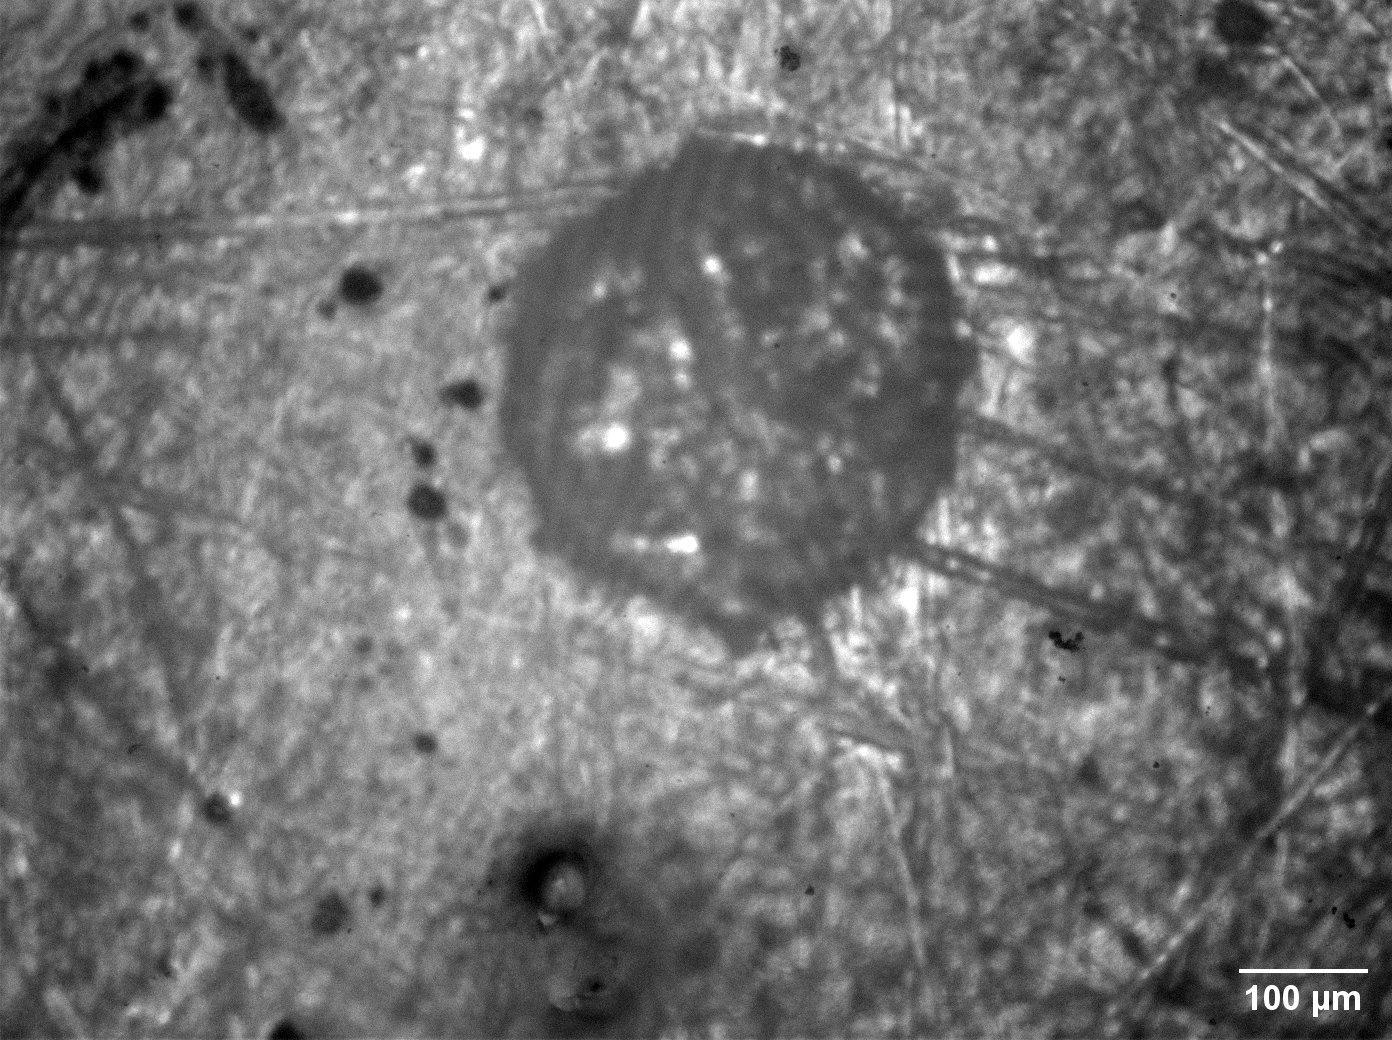
\includegraphics[width=7.5cm]{50_1_25p_3min_after_plasma_rommtemp.ome}
		\caption{}
	\end{subfigure}
	\begin{subfigure}[]{0.45\textwidth}
		\centering
		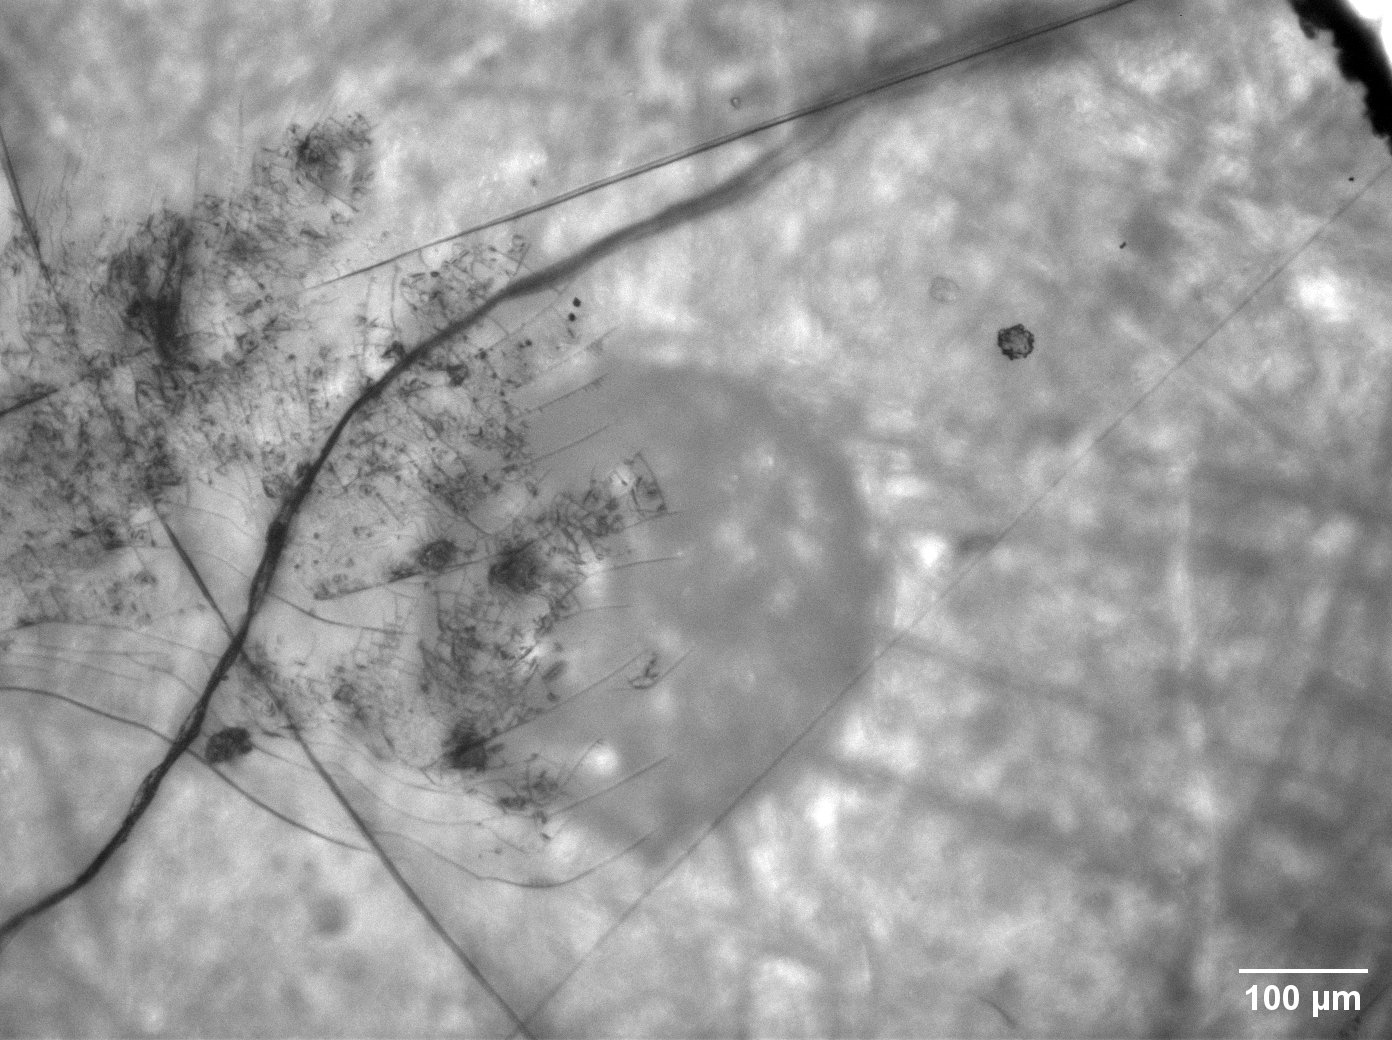
\includegraphics[width=7.5cm]{50_1_100p_3min_after_plasma_rommtemp.ome}
		\caption{}
	\end{subfigure}
	\begin{subfigure}[]{0.45\textwidth}
		\centering
		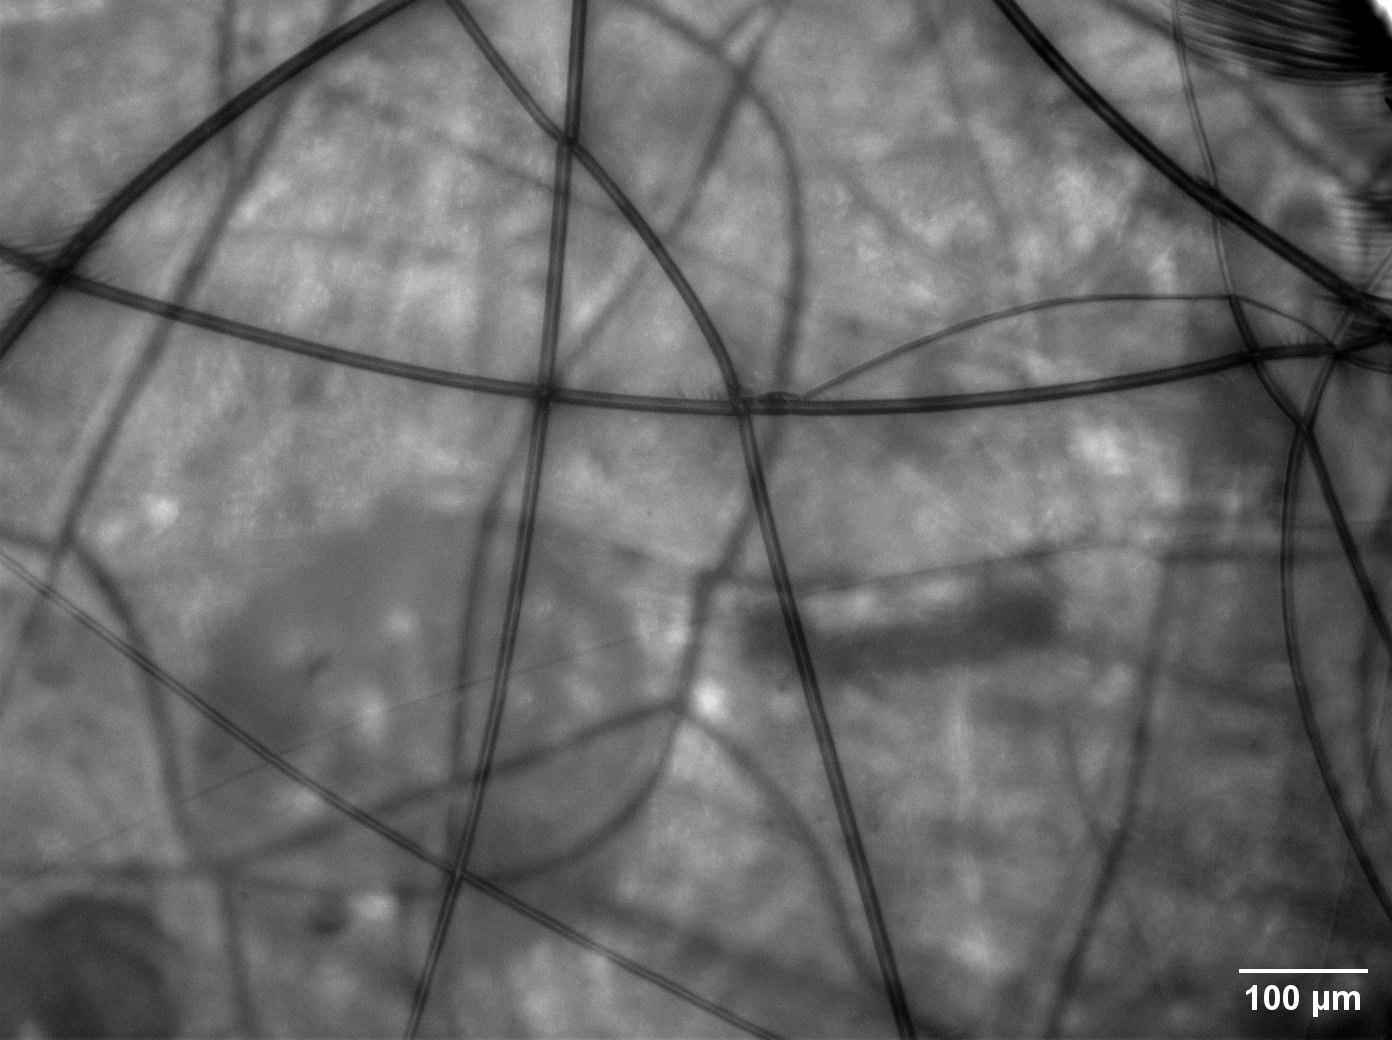
\includegraphics[width=7.5cm]{50_1_100p_10min_after_plasma_rommtemp.ome}
		\caption{}
	\end{subfigure}
	\caption{Comparison of different Plasma activation on PDMS with 50:1 mixture ratio. In (a), $25\,\%$ Power at \SI{3}{\minute} leads to no crack formation. in (b), $100\,\%$ Power at \SI{3}{\minute} leads to cracks. Increasing the duration to \SI{10}{\minute} at $100\,\%$ power increases the cracks. The cracks indicate increased brittleness of the surface.}
	\label{fig:Vgl50:1Plasma}
\end{figure}

\FloatBarrier

\section{Experiments at cryogenic temperature}

%TODO AN PASSENDE STELLE
To try out the separating with the finger in a repeatable manner, a core process is established. The sample is plunge-frozen with fluoresceine water or taken out of the storage and placed on the work surface in the bath. The copper shuttle is placed in the harbor. With HFE, the sample is placed in the middle of the shuttle. The HFE helps the sample to stay in place before fixation. The window brace is placed on top and screwed down. The now prepared shuttle is transported quickly to the microscope for pre-imaging. When the transfer is not possible within seconds, the shuttle is placed in a portable container with liquid nitrogen. After microscopy, the sample is placed into the bath unter the cooled finger. 

\subsection{Preparation of samples}
%TODO

In sample preparation for cryo microscopy, specimens such as cells are frozen inside a thin ice layer. the specimen can be stained with fluorescein before freezing for later observation with cryo light microscopy. Also a sample can be prepared to study with cryo-transmission electron microscopy (cryo-TEM). cryo-TEM allows us to see samples in an hydrated state. This is only possible in cryo-TEM, as liquid water would evaporate in vaccuum \cite{Danino.2012}.

For cryo light microscopy and cryo-TEM, plunge-freezing is used in sample preparation \cite{Danino.2012} \cite{Faoro.2018}. This can be done either manually or with a plunge-freezer, with comparable results. In practice, using a plunge-freezer gives more consistent results.

To successfully plunge-freeze a sample, following steps are taken: First, the slide is held by tweezers. Then a \SI{2}{\milli\liter} water drop containing the specimen is pipetted onto the hydrophilic slide. The water droplet is blotted with filter paper, creating a thin film of water which evaporates quickly. The tweezers holding the slide is shot in cold liquid under \SI{-140}{\degreeCelsius}, typically liquid ethane. The rapid temperature drop freezes the water into a thin vitrificated layer of ice. vitrificated ice has no crystal structure.

For example, thin sapphire slides or a metal grid with a film are commonly used. Also the liquid which is used to freeze the sample should not possess the Leidenfrost effect, which prevents instant contact of the sample with the cold liquid. As liquid nitrogen is possessing the Leidenfrost effect, other coolants like liquid ethane are used.

For long time storage small containers with space for three $\varnothing$\SI{5}{\milli\meter} samples are designed (Fig. \ref{fig:transportbox}). These are 3D Printed, modified version of grid boxes. a grid box cap is screwed on top with a special tool. Inside the bath, grid boxes and these 3D-printed container fit into the indent. The cap is screwed next to the container, clamping it down to the work surface. Also the container are interoperable with tools used for grid boxes. This allows long term storage of samples with \SI{5}{\milli\meter} diameter.

%TODO mentioning dass Samples die hier untersucht werden ncith vitrifiziert sind

\subsection{Inverted microscope}

The used microscope setup is a prototype based on an uninverted microscope. As using more inverted light microscopes are considered for usage in cryogenic temperature, the setup is analized and some common issues and possible fixes are proposed.

To take pictures, a two-fold and 5-fold objective is used. The 5-fold objective fits between the microscope and glasses assembly without a significant gap. However, to fit the 2-fold objective the glasses assembly needs to designed thinner. With the increased gap between objective and glasses assembly, more ambient light is lighting the sample. This decreased the visibility of fluorescence on samples. With the increased field of view with the 2-fold objective, total reflection of the two glass panes in the glasses assembly is inducing strong noise in the pictures. Also the access hole to the harbor is a bit too small.
To reduce noice and increase the harbor access, the glasses assembly is fixed tilted to the box by adding spacers. In future, the glasses assembly needs to be redesigned to fix all those issues.

To take detailed pictures of the sample, an inverted microscope is modified for cryo- microscopy (fig. \ref{fig:Mikroskop}). A box with a copper heat sink is fixed to the bottom of the stage. The box is supplied with cold nitrogen gas to cool the heat sink (fig. \ref{fig:boxmikroskop}). A haven is fixed to the heat sink and placed over the objective. The haven is temperature controlled to \SI{-140}{\degreeCelsius}. the "glasses" component keeps the light path between haven and objective clear from ice and fog. It contains two thin and parallel glass panes. Warm nitrogen gas is routed between the glass panes and out between the lower glass pane and objective.

The microscope is able to image fluorescence light. For this, filters are swapped between real light images and fluorescence images. A 2 fold and and later 5 fold objective is used for imaging. %TODO hier müsste dann das mit dem Kippen der brille noch hinzukommen

\begin{figure}[hbt!]
	\centering
	\begin{overpic}[width=10cm]{Microscope}
		\put(24, 45){\vector(1,0){10}}
		\put(24, 45){\makebox(0,0)[r]{cooled box}}
		\put(15, 50){\vector(1,0){10}}
		\put(15, 50){\makebox(0,0)[r]{frame}}
		\put(35, 25){\vector(1,0){5}}
		\put(35, 25){\makebox(0,0)[r]{objective}}
		\white
		\put(52, 33){\vector(-1,0){10}}
		\put(52, 33){\makebox(0,0)[l]{"glasses"}}
		\put(55, 52){\makebox(0,0)[c]{cold nitrogen gas supply}}
		\put(50, 75){\makebox(0,0)[b]{stage}}
		\put(59, 40){\vector(-1,0){10}}
		\put(59, 40){\makebox(0,0)[l]{gas outlet}}
		\put(32, 35){\vector(1,0){10}}
		\put(32, 35){\makebox(0,0)[r]{access shuttle}}		
	\end{overpic}
	\caption{Modified microscope for cryo microscopy.}
	\label{fig:Mikroskop}
\end{figure}

\begin{figure}[hbt!]
	\centering
	\input{../images/Zeichnung_Box_mikroskop.pdf_tex}
	\caption{cross-section Box to keep the shuttle and sample cool. The harbor is fixed on the copper heat sink. The heat sink is cooled by cold nitrogen gas flowing trough the box keeping the heat sink cool. Below the box lid, the cold nitrogen gas is exhausted into the environment. The glasses assembly keeps the light path clear}
	\label{fig:boxmikroskop}
\end{figure}

In general, fitting the sample into the harbor is difficult. The cold gas is exhausted over the access to the harbor. The exhausted cold gas results in fog and locally reduces oxygen. The big stage and cooled box on top reduces visibility to the access point. In future, the exhaust should be pointed away from important access points.

Ice frozen to the assembly can also damage the microscope. Especially when the setup warms back up to room temperature, the ice melts and water drops onto important parts. Therefore, the objectives should be designed water proof. Gaps should be closed as much as possible to avoid water entering the inside of the microscope.

The shuttle allows easy transportation and access to the sample. The sample is clamped down by the "window" brace (fig. \ref{fig:shuttle}). The window brace is fixed with two screws to the shuttle, holding the sample in place. A center hole in the window gives access to the top side of the sample for microscopy and finger. In the copper shuttle a thread is placed. With a long threaded metal rod the sample is transported between assemblies.

\subsection{Baths and finger}

Two different setups are used. First, the setup with "finger" and "bath" is used. Second, for additional data, a modified version of the setup with the pulling machine is used. This allows the measurement of the actual tensile strength on the sample. 

The finger is made of two main parts: The first part is a metal rod with a flat tip (Fig. \ref{fig:querschnittfinger}). The rod is cooled with cold nitrogen gas. Near the tip, the rod is temperature controlled with a Pt1000 used as a temperature sensor and a heater. The second part is a 3D printed structure, containing the outer layer and routing of the cold gaseous nitrogen. Inside the 3D printed structure, the cold nitrogen gas is directed from the inlet downwards around the metal rod in an inner mantle for cooling. Then, the cold gas is redirected upwards flowing through an outer mantle for additional cooling. Afterwards, the gas exits through the output.

\begin{figure}[hbt!]
	\centering
	\input{../images/ZeichnungFinger.pdf_tex}
	\caption{A cross-section of the "finger" assembly. The metal rod is cooled with cold nitrogen gas. the gas is routed from the inlet around the metal bar onto an outer layer to the outlet. The metal rod is temperature controlled by a Pt1000 temperature sensor and a heater. With HFE 7200 is applied to the tip, the finger can attach to a surface at cryogenic temperatures and apply force. }
	\label{fig:querschnittfinger}
\end{figure}

The cold nitrogen gas is supplied by a liquid nitrogen tank. Heaters placed inside the tank evaporate the liquid nitrogen. Cold nitrogen gas leaving the tank is routed by \SI{6}{\milli\meter} pneumatic tubing to the finger inlet. On the inlet and outlet of the finger, Festo connectors are mounted to allow easy dis- and re-connection of \SI{6}{\milli\meter} tubes. Cold nitrogen gas which passed through the finger are exhausted by outlet tubing into the atmosphere.

The finger is mounted on a three stages. These stages allow fine adjustment of the finger position in X,Y and Z axis (fig. \ref{fig:FingerStages}). Also, when the finger is attached to a surface, force can be applied by moving the stages in either direction. Additionally the stages are mounted on a track. The track allows fast movement along one axis to make assemblies below the finger reachable. Whenever the finger is used, the assembly is clamped down to the track to prevent additional movement.

\begin{figure}[hbt!]
	\centering
	\begin{overpic}[width=10cm]{Finger_Stages}
		\white
		\put(20,37){\makebox(0,0)[c]{Track}}
		\put(37,90){\vector(1,0){10}}
		\put(37,90){\makebox(0,0)[r]{Stage Z-axis}}
		\put(75,45){\vector(0,-1){10}}
		\put(75,45){\makebox(0,0)[b]{Stage X-axis}}
		\put(36,8){\vector(1,0){10}}
		\put(36,8){\makebox(0,0)[r]{Stage Y-axis}}
		\put(67,88){\vector(-1,0){10}}
		\put(67,88){\makebox(0,0)[l]{Finger}}
		\put(70,65){\makebox(0,0)[c]{Bath}}
	\end{overpic}
	\caption{Stages to precisely manipulate the finger tip in X, Y and Z direction. When the finger is not in use, it is moved along the track to allow access to assemblies below.}
	\label{fig:FingerStages}
\end{figure}

On the tip of the finger, Ethoxynonafluorobutane, also called Hydrofluorether 7200 (HFE) is used throughout all experiments. HFE is used as cooling agent \cite{Tsai.2005} as well as an cryoimmersion fluid \cite{Faoro.2018b}. HFE has temperature dependent characteristics. At freezing point, HFE reaches a viscous state before reaching a firm solid state. This temperature dependency allows to first apply the HFE at higher temperatures with low viscosity and pull on the sample at lower temperatures with high viscosity.

The temperature regulation of the finger has three modes: First the "unglue" mode which regulates the Temperature to \SI{-140}{\degreeCelsius}. HFE has a low viscosity, which allows the application of HFE. Also separating the finger off the sample without transferring force is possible. Second, in "glue" mode the shuttle and the finger are cooled to \SI{-160}{\degreeCelsius}. HFE hardens and force can be applied to detach the ice layer. Third, "thaw" cleans the finger by heating the tip to \SI{20}{\degreeCelsius}, evaporating everything stuck on the finger.

In the beginning a smaller bath is used (Fig. \ref{fig:KleinesBad}). The small bath contains an elevated work surface. Embedded in the work surface are indents which fit container holder. Three elevated baths are installed on the elevated floor. They are temperature controlled for containing other Liquids or tools at different temperatures. Also a Haven for a shuttle system is installed. The small baths and the haven are separated from the elevated floor with an insulating layer. The bath is filled with liquid nitrogen covering the work surface. The whole bath is insulated by Nitrogen gas flowing inside the 3D-printed shell of the bath. The warm nitrogen gas is expelled from the brim, flowing from the outer edge radially to the middle rotation axis.

The usage of the small bath in combination with the finger has limitations: First, the space in the small bath is small. The finger can be moved along the track, but the space left still limits work with pincers. Additionally, the smaller temperature controlled baths are not needed when using the finger, therefore taking up much needed space. Also the Shuttle needs to be tilted in a specific angle to dock and undock the shuttle. The work flow also allows only one shuttle at once, limiting throughput. Also liquid nitrogen needs to be refilled often since the bath can only hold a smaller volume.

\begin{figure}[hbt!]
	\centering
	\begin{overpic}[width=10cm]{SmallBath}
		\white
		\put(40,25){\vector(1,1){10}}
		\put(40,25){\makebox(0,0)[r]{shuttle haven}}
		\put(20,45){\vector(1,0){15}}
		\put(20,45){\makebox(0,0)[r]{tool bath}}
		\put(73,35){\vector(-1,1){10}}
		\put(73,35){\makebox(0,0)[l]{ethanol bath}}
		\put(73,27){\vector(-1,1){10}}
		\put(73,27){\makebox(0,0)[l]{HFE bath}}
		%\put(49,76){\vector(-0.15,-1){3.4}}
		%\put(51,76){\vector(0.15,-1){3.4}}
		\put(48,65){\vector(-0.25,-1){2.8}}
		\put(52,65){\vector(0.25,-1){2.8}}
		\put(50,65){\makebox(0,0)[b]{container holder}}
		%\put(75,78){\vector(-2,-1){10}}
		%\put(76,78){\vector(-1,-2){4.5}}
		\put(75,72){\vector(-1,0){10}}
		\put(79,68){\vector(-1,-1){3.5}}
		\put(75,72){\makebox(0,0)[lt]{gas outlets}}
		\put(75,72){\makebox(0,0)[lb]{nitrogen}}
		\put(30,62){\vector(1,-1){10}}
		\put(30,62){\makebox(0,0)[rb]{work surface}}	
	\end{overpic}
	\caption{Small bath used for sample preparation. This bath is combined with the finger. A major drawback of use with the finger is the lack of space inside the bath. To solve this issue, a bigger bath is constructed.}
	\label{fig:KleinesBad}
\end{figure}

During this master thesis, a second bigger bath is build (Fig. \ref{fig:GroßesBadMitFinger}). In general, the structure is similar. It also uses an elevated floor as a work surface. The work surface is fabricated out of two plates screwed together and fixed to the brim with 3D-Printed hooks. Indents are formed by holes in the upper plate. No baths are installed, but the space is reserved for later addition. Two harbors are mountable for parallel work on two separate shuttles. The harbors are screwed on an aluminum block with Pt-1000 temperature sensors and heaters for temperature regulation. Between the aluminum block and the work surface, a 3D-printed insulating spacer is placed. Also both harbors can be mounted either flat or in an angle, depending of the 3D printed spacer. The bath is insulated with styrofoam and a rim with holes for warm nitrogen gas is placed on top. The holes are places along the inside of the long perimeter.

\begin{figure}[hbt!]
	\centering
	\begin{overpic}[width=10cm]{BigBathWithFinger}
		\white
		\put(24, 35){\vector(1,1){10}}
		\put(24, 35){\makebox(0,0)[t]{shuttle haven}}
		\put(46, 31){\vector(-1,1){10}}
		\put(46, 31){\makebox(0,0)[t]{temp. controlled aluminum block}}
		\put(25, 75){\vector(1,0){10}}
		\put(25, 75){\makebox(0,0)[r]{"finger"}}
		\put(15, 19){\vector(-1,-1){10}}
		\put(15, 19){\makebox(0,0)[l]{inlet warm nitrogen gas}}
		\put(50, 15){\vector(0,1){5}}
		\put(50, 15){\makebox(0,0)[t]{hole for refilling}}
		\put(40, 85){\vector(-1,1){5}}
		\put(40, 85){\makebox(0,0)[l]{cold nitrogen tubing}}
		\put(15, 58){\vector(0,-1){15}}
		\put(16, 58){\vector(0,-1){10}}
		\put(16, 58){\makebox(0,0)[b]{gas outlets nitrogen}}
		\put(32, 52){\vector(0,1){5}}
		\put(32, 52){\makebox(0,0)[t]{container holder}}
		\put(17, 88){\vector(0,-1){5}}
		\put(17, 88){\makebox(0,0)[b]{connection "finger" to stage}}
	\end{overpic}
	\caption{Big bath with finger assembly. Inside the bath samples are prepared. When applying forces with the finger, the sample fixed on a shuttle is held in place by the harbor.}
	\label{fig:GroßesBadMitFinger}
\end{figure}

\subsection{Setup pulling machine for cryogenic tests}

To allow tests at cryogenic temperatures with the pulling machine, the setup is modified to allow fitting a bath and the "finger" to the pulling machine. The big bath is used with a flat harbor. An outer frame is used and modified to hold the bath. The bottom clamp is removed and the Bath is fixed over the bottom attachment. The top part is used with the same load cells, but with a bigger clamp. The "finger" 3D printed shell modified with a flat outer profile for clamping and clamped onto the top. \SI{90}{\degree} festo tubing is used to connect the cold nitrogen gas supply. A power source and a temperature regulator is again used. 

%TODO BILD

Compared to the "finger" setup with stages, the finger only moves up and down. The Alignment is done by moving the bath by loosening the screws on the frame. Also new "window" parts are waterjet cut. The new "window" has a bigger central hole for easier alignment.

As the tensile testing machine is set up in a separate room, the samples are prepared in the laboratory next to the microscope. The small bath is used for sample preparation. The process is the same as all detachment trials with the finger. 

\begin{figure}[hbt!]
	\centering
	\begin{subfigure}[]{0.45\textwidth}
		\centering
		\input{../images/Zeichnung_shuttle.pdf_tex}
		\caption{Shuttle for transporting a sample between bath and microscope. The window is clamped down by screws to the copper shuttle, holding the sample in place. the center hole in the window gives access for microscopy and finger.}
		\label{fig:shuttle}
	\end{subfigure}
	\begin{subfigure}[]{0.45\textwidth}
		\centering
		\input{../images/Zeichnung_transportbox.pdf_tex}
		\caption{Small 3D-printed transport box for three samples. A cap is screwed onto the central thread. These boxes fit into storage units. The design is based on a commonly used storing system.\newline\newline}
		\label{fig:transportbox}
	\end{subfigure}
	\label{fig:shuttleandtransportbox}
\end{figure}

This setup has a lot of limitation. Aligning the finger is very difficult, as the screws are hard to reach in cold temperature. When cooling, the previous alignment ist lost as the coldness distort the setup. Also little movement at the finger has maximum effect on the sample and alignment. touching the tubes can loosen the sample and/or the setup needs to be new aligned. Even a bigger window is not enough. Errors in alignment and therefore gluing to the border of the window and loosening through movement are the two biggest error sources in this setup. So the old setup is used in further experiments to eliminate big error sources.

\subsection{Factors observed influencing detachment with finger}

%TODO

\subsubsection{Volume of Hydrofluorether on finger}

%First the volume of HFE is evaluated. High dosages of liquid HFE can spread underneath the frame holding the sample, leading to an inefficient force distribution. Also a thick glue layer take less tensile force, leading to a reduction of maximum force on the sample. Too little HFE will not connect the finger to the sample. Additionally, the dosaging of glue ia found to be a challenge.

Using the correct amount of HFE on the finger tip is important for higher repeatability. Too little HFE will not bind to the finger and sample. Using too much HFE results either in a thicker layer, or the HFE flows between window and sample. as the cohesion of the HFE is considerably lower than the sample and the finger, a thick layer is prone to breaking before the ice layer. HFE under the window clamp will redirect a part of the force, making the sample more stable. This makes detaching also harder.

At the start, the HFE was applied with a pincer. The HFE is given in a cold bath at \SI{-140}{\degreeCelsius}. HFE gets more viscous at colder temperatures and is evaporating much slower. The thickened HFE is now scooped with pincers onto the tip of the finger.

%As an effort to determine the volume of HFE a pipette is used. The HFE is pipetted at room temperature onto the cold finger. When HFE is applied onto the desired surface, around \SI{4}{\micro\liter} has already evaporated. Also, only HFE on the flat surface facing the sample is usable.

The HFE is dosaged with a pipette onto the tip of the "finger". While pipetting, around \SI{4}{\micro\liter} of HFE is evaporating. Based on this knowledge, dosaging $4.10\,\mu l$, $4.30\,\mu l$ and $4.50\,\mu l$ is compared and a video is taken for later comparison.

The videos show that pipetting HFE is not reliable. The visible HFE volume on the tip does not correlate with the dosaged volume. On reason is a difference in the volume of HFE evaporating while applying. Also some HFE may be placed on the side of the tip. When using the finger, only the HFE on the flat tip is effective.

Another way to determine the Volume of HFE on the finger is by analyzing pictures of the finger with HFE. The volume is calculated with the contact angle on the finger and the area covered in HFE. With the knowledge if the HFE spreads too much or not being attached properly to the sample, a range can be given where success is more likely. Still, other factors like temperature or the gap between sample and finger can influence the result.

Still, a visual estimate for the correct glue dosage is made by calculating the drop volume out of camera images. Two exemplary Pictures of an upper and lower limit of glue dosages is picked (Fig. \ref{fig:rangeHFE}). Then the volume is calculated with a formula for the volume of a spherical section. All needed components are calculated out of the estimated contact angle of the glue $\alpha \approx 45°$ and the tip diameter of $d = 1.68\,mm$. For the lower range a reduction of $d$ by a factor of $\frac{2}{3}$ is assumed as the drop is not covering the whole tip. The resulting volume range of the HFE is $ 0.11\,\mu l \gtrapprox V \gtrapprox 0.38\,\mu l $.

\begin{figure}[hbt!]
	\centering
	\begin{subfigure}[]{0.45\textwidth}
		\centering
		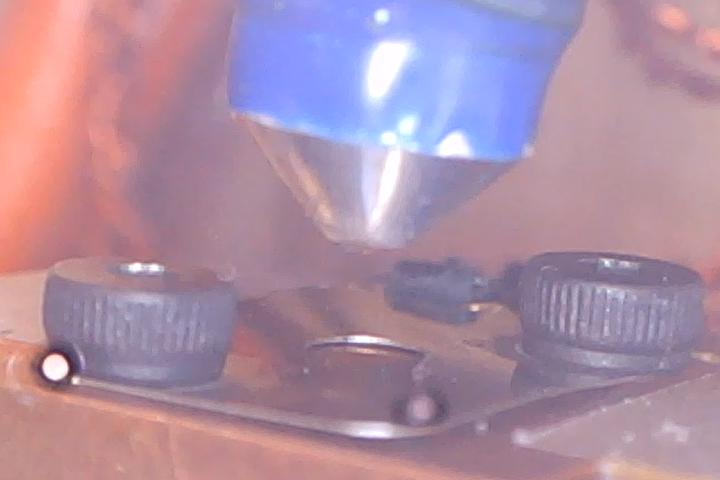
\includegraphics[width=7.5cm]{LowerLimit_quadrat}
		\caption{lower limit HFE volume}
	\end{subfigure}
	\begin{subfigure}[]{0.45\textwidth}
		\centering
		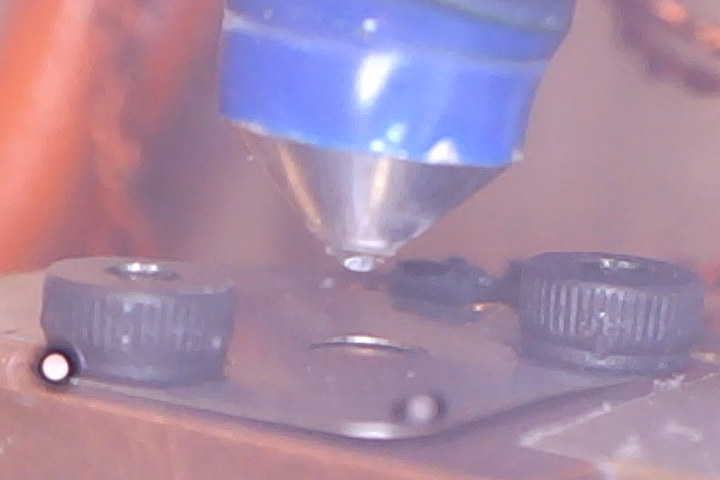
\includegraphics[width=7.5cm]{UpperLimit_quadrat}
		\caption{upper limit HFE volume}
	\end{subfigure}
	\caption{Visual representation of the range of dosages which are the most reliable. less HFE than the lower limit is more likely to not attach to the sample properly. more HFE than the upper limit will spread under the "window" brace or results in a thick HFE layer with less tensile strength.}
	\label{fig:rangeHFE}
\end{figure}

\subsubsection{Temperature}

HFE has a freezing point of \SI{-138}{\degreeCelsius}. Below the freezing point, HFE gets increasingly viscous first. at a certain point, the HFE gets brittle and cracks start to form by decreasing temperature. Between the freezing point and the point of cracking, HFE is usable similar to glue. With a temperature near the freezing point, HFE can spread over the surface. At lower temperatures, HFE gets hard enough to hold the finger to the upper ice layer.

As HFE is getting harder with temperature, lower temperatures in the "glue" state could allow higher forces on the ice layer. Still, the point where HFE starts to crack will decrease the tensile strength. To test this hypothesis, HFE is examined at temperatures below the freezing point.

To test the viscosity and crack formation of HFE below freezing temperature, HFE is given into a small temperature controlled bath. The temperature is regulated from \SI{-150}{\degreeCelsius} to \SI{-170}{\degreeCelsius} in \SI{5}{\degreeCelsius} steps. After reaching \SI{-170}{\degreeCelsius}, the temperature is regulated back to \SI{-150}{\degreeCelsius} in \SI{5}{\degreeCelsius} steps. Changes in HFE when cooling and heating up are observed. A needle is put in the HFE to induce forces and subjectively test the viscosity of HFE at all temperatures.

At \SI{-150}{\degreeCelsius} to  \SI{-155}{\degreeCelsius} , the HFE is still only lightly viscous . the needle is not held up by the HFEs viscosity. At \SI{-160}{\degreeCelsius} to  \SI{-165}{\degreeCelsius} the HFE is viscous enough so that the Needle is hold up by the HFE. The Needle can be pulled out and the HFE is closing the gap. Also with enough force, the Needle can penetrate the HFE. also no cracks formed so far. At \SI{-170}{\degreeCelsius}, HFE hardens further. The HFE is still viscous. Wiggling the Needle in the HFE can result into cracks. Then the Needle can be easily pulled out. Under \SI{-170}{\degreeCelsius}, Cracks form without inducing forces in the HFE.

Heating the cracked HFE up leads to the cracks eventually disappearing. at \SI{-165}{\degreeCelsius}, first cracks disappear, but a many remain. The cracks left are still lowering the mechanical stability of the HFE. Heating up to \SI{-160}{\degreeCelsius} results in less cracks, but some still remain. A temperature of \SI{-150}{\degreeCelsius} will result in cracks completely disappearing.

In conclusion, maximum load can be applied at \SI{-165}{\degreeCelsius}. Higher temperatures result in lower viscosity, which lowers the maximum stress before HFE breaks. At \SI{-170}{\degreeCelsius}, cracks will form, lowering the maximum stress.

%TODO
To test how applicable the temperatures are with the "finger" setup, pulling tests are done as described in section

 except the temperatures of the finger is lowered to \SI{-165}{\degreeCelsius} and \SI{-170}{\degreeCelsius} in the "glue" state. With attention to proper insulation and no leakages of cold nitrogen gas, \SI{-165}{\degreeCelsius} is quickly reached and is held stable by temperature regulation over a time span of minutes. Still, the setup is not very reliable as new leaks can form and changing of tanks/tubings can lead to new leaks. These leaks are spotted only when the finger is already cooled. To fix leaks, the setup needs to warm up. \SI{-170}{\degreeCelsius} can sometimes be reached with the finger, but holding the temperature stable is not possible. 

When cooling down to the desired temperature with the "glue" state, liquid nitrogen is refilled to increase cooling. When refilling and cooling at the same time, rapid cooling happens when liquid nitrogen touches the shuttle directly at refilling. With this, the Temperature can shortly drop below \SI{-170}{\degreeCelsius}. This induces cracks in HFE, lowering the tensile strength. If this happens, the Sample and finger can be heaten up to the "unglue" state at \SI{-140}{\degreeCelsius} and the cracks disappear. Then cooling can start again.

In conclusion, the finger "glue" temperature is most effective at \SI{-165}{\degreeCelsius}. Still, the reliablility suffers trough leaks, longer tubing and inproper insulation. For better repetition, a temperature of \SI{-160}{\degreeCelsius} is also used in experiments.

\subsubsection{Applied Tensile force to HFE}

To additionally measure the force applied of the finger, the pulling machine is used in combination with the finger. In the lab, the small bath is used for sample preparation. after microscopy, the sample is transported to the pulling machine. the big bath is fixed on the bottom of the pulling machine. on top, the finger is clamped into the shackle and aligned to the shuttle. The process is still as previously stated. 

Over all pulls, the HFE can transfer a maximum force of $1.30\pm0.49\,\si{\newton}$. The exact size of the area which experienced the force is unknown. Additionally, the force distribution is uneven (e.g. like Fig. \ref{fig:ZeichnungBerechnungStress_c}). A worst case and a best case which are easily calculated can be determined. as best case, all force is evenly distributed under the area of the finger (Fig. \ref{fig:ZeichnungBerechnungStress_a}). With this assumption, the Area is equal to the finger tip area. The worst case is an even distribution over the whole surface (Fig. \ref{fig:ZeichnungBerechnungStress_b}). The surface is clamped by the window. So the inner diameter of the Window is the worst case area. In reality, the Force is somewhere in between (Table \ref{table:VerschAbschätzungenStressFinger}).

\begin{figure}[hbt!]
	\centering
	\begin{subfigure}[]{0.3\textwidth}
		\centering
		\input{../images/ZeichnungBerechnungStressFinger_Finger.pdf_tex}
		\caption{}
		\label{fig:ZeichnungBerechnungStress_a}
	\end{subfigure}
	\begin{subfigure}[]{0.3\textwidth}
		\centering
		\input{../images/ZeichnungBerechnungStressFinger_Window.pdf_tex}
		\caption{}
		\label{fig:ZeichnungBerechnungStress_b}
	\end{subfigure}
	\begin{subfigure}[]{0.3\textwidth}
		\centering
		\input{../images/ZeichnungBerechnungStressFinger_Combined.pdf_tex}
		\caption{}
		\label{fig:ZeichnungBerechnungStress_c}
	\end{subfigure}
	\caption{Different worst- and best case examples of force distribution on sample. In best case, the force is concentrated on the small area around the finger tip (a). In worst case, the force is evenly spread over the whole sample (b). In reality, the force distribution is between shown extremes. One example of a realistic force distribution is shown in (c).}
	\label{fig:ZeichnungBerechnungStress}
\end{figure}


\begin{table}[hbt!]
	\centering
	\begin{tabular}{|l|l|l|}
		\hline
		Area used & Area Size & Tensile Stress\\
		\hline
		\hline
		Finger & \SI{2.217}{\milli\meter\squared} & $585.4\pm219.4\,\si{\kilo\pascal}$ \\ 
		\hline
		Small Window & \SI{4.91}{\milli\meter\squared} & $264.3\pm99.1\,\si{\kilo\pascal}$ \\ 
		\hline
		Big Window & \SI{12.56}{\milli\meter\squared} & $103.3\pm38.7\,\si{\kilo\pascal}$ \\ 
		\hline
	\end{tabular}
	\caption{Tensile stress and size of area used to calculate the tensile strength of the finger setup. In worst case, the force is distributed over the whole "window" size(Fig. \ref{fig:ZeichnungBerechnungStress_b}). In best case, the force is only distributed on the "finger" tip (Fig. \ref{fig:ZeichnungBerechnungStress_a}). The real value is between those extremes.}
	\label{table:VerschAbschätzungenStressFinger}
\end{table}

\FloatBarrier

\subsubsection{Direction of force}

The direction of force can increase the likelihood of a successful separation. For example, to remove a suction cup from a flat surface, using tensile force by pulling will take a higher maximum force than by sliding the suction off the surface by shear forces. The same could apply to the sample. To test this hypothesis, separation tests are done by applying forces differently.

%TODO komischer absatz
Tensile mode and shear mode can be applied by the finger. Tensile mode is the easiest to apply with the finger. Also HFE is able to withstand some tensile forces. But for separating layers, this mode could take more force than applying tensile forces, depending on the bottom layer. In research, PDMS shows less adhesion forces on ice if tensile stress is applied \cite{IbanezIbanez.2022}. Still, HFE stability to shear stress is not known. Additionally, the sample is clamped down to the top. This does not allow the ice surface to slide off without breaking.

In most experiments, the shuttle is tilted around 15 degrees for easier access to the shuttle. The finger is also tilted so the tip surface is parallel to the sample. To apply force, the finger is pulled by stages in either X, Y, or Z direction. For each direction, the resulting stress can be split into tensile and shear stress. In Z direction, mostly tensile stress is applied (Fig. \ref{fig:tensilevsshear} (a)). in X direction, mostly shear stress is applied (Fig. \ref{fig:tensilevsshear} (b)). In Y direction, only shear stress is applied. But detached pieces moving in Y direction will collide with the clamped down part of the ice layer. This could shatter the ice layer or take more force. Additionally, the sample is clamped down only by friction, strong forces in Y direction could slide the sample inside the shuttle. For this reason, only X and Z direction are tested.

\begin{figure}[hbt!]
	\centering
	\input{../images/Zeichnung_finger_Tensile_vs_Shear.pdf_tex}
	\caption{The shuttle is tilted inside the bath at \SI{15}{\degree}. Pulling on the sample in Z direction (a) results in mostly tensile stress and some shear stress on the sample. Pulling in X direction (b) results in mostly shear stress and some tensile stress.}
	\label{fig:tensilevsshear}
\end{figure}

In experiments, less force was transferred when pulling in X direction. This is detected by the manually applied force to the stage. No separation or breaks are confirmed in those tests. This suggests that HFE is susceptible to shear forces. Therefore, detachment using another force direction is more unlikely. 

\subsubsection{Positioning}
\label{section:positioning}

Before attaching the finger to the sample, the finger is positioned with the stages. At positioning, two different errors can occur: first, the finger is incorrectly positioned in X and Y direction over the sample. The HFE will spread partially on and under the window brace. The second error is a too small or too big gap between finger and sample in Z-direction. 

An incorrectly position in X or Y direction is expected to massively effect detaching. Depending on the overlap, the force is transferred mostly to the window brace than to the sample. This will lead to an unsuccessful detachment. With the setup of a stage in each axis, the positioning is easily corrected. Alternatively, a window brace with a bigger central hole makes positioning easier.

The gap between sample and "finger" is sometimes hard to estimate. The HFE volume influences the optimal gap size to avoid pressing the HFE between sample and "window". On the other hand, HFE is shrinking between temperatures used at attaching and pulling. Also the cohesion of HFE is low, so keeping a bigger gap will also influence the maximum force. Therefore, the gap size is not completely isolatable with the HFE volume.

When attaching, the right distance between sample and "finger" helps increasing the tensile force which can applied to the sample. As discussed in section \ref{section:positioning}, two types of positioning errors can occur: The positioning over the sample and the gap between sample and "finger". The first error can be corrected by stages in X and Y directions. The other error also depends on the HFE volume. With little volume, There is no risk of HFE spreading between sample an "window". With a high volume, Decreasing the gap can result in HFE spreading under the window brace if the "finger" is lowered too much. On the other hand, leaving a big gap between "finger" and sample results in a thicker HFE layer which takes less tensile forces.

\subsubsection{observed error sources}

The duration of time between reaching the "glue" state from the "unglue" state makes disconnecting before pulling more likely. The sample is cooled with the "finger" on top as well as by the harbor cooled with liquid nitrogen. Best case is the same cooling rate of "finger" and harbor. In practice, the cooling of the "finger" is faster. This also leads to successful attaching. If for example major leaks occur in the cold nitrogen gas supply, the cooling rate of the "finger" is slower than the harbor. In those cases, the "finger" does not stay attached to the sample. A theory is that HFE gets more viscous on the sample than on the "finger". While the HFE is perfectly adhering to the samples surface. Additionally, the HFE loses volume due to cooling. The HFE on the tip of the "finger" is able to fill out the missing volume and thin out around the finger due to gravity. With enough time, this could the HFE enough that the finger is not properly attached anymore. (NICHT SO DIE BESTE THEORIE; EIGENTLICH BEI GRO?ER LÜCKE?)

The formation of Ice inside the bath is largely inhibited through the Nitrogen Gas inlets. The nitrogen is forming a barrier to the atmosphere which contains humidity that turns into ice at cold temperatures. However, through turbulence and the finger, some ice can form inside the bath. 

In some experiments, high buildup of additional ice is observed on the sample. The additional ice is looser, reducing the possible grip onto the desired ice layer. The formation is traced back to a leakage in the finger. The tolerances between 3D printed part and metal bar should be able to seal the gap airtight. But trough changing out parts, the tolerances are looser, allowing a weak cold nitrogen current right on the sample. There are two possibility where the humidity itself is coming from: The cold nitrogen gas itself could contain some humidity. Second through additional turbulence, more air is sucked through the barrier. The air is directed directly on the sample, causing more ice buildup. To avoid this, the gap is sealed tight with twinsil dublicating silicone typically used for dental application.

\subsection{Tensile testing of engineered layer with finger}
%TODO

To lift off a piece of the ice layer, the ice layer must be broken in some way. thicker ice layers are expected to be harder to break than thinner ones due to the bigger cross section. Also amorphic vitrified ice is expected to be more stable than crystallized ice.

Initially, to save time for experiments, the samples are freezed manually in liquid nitrogen, as described before. However, the ice layers are less consistent compared to plunge freezing, resulting in mostly thicker ice layers compared to plunge freezing. also as the sample is frozen in liquid nitrogen, the leidenfrost effect is inhibiting the formation of vitrified ice.

In experiments, the used glass slide and freezing method does not produce vitrified ice. Therefore the influence of vitrification is not observed. The thickness of the ice is also not measured directly. 

To compare the influence of hand freezing and plunge freezing, results of lifting off samples frozen with both methods are compared. No other factors are varied in those experiments. In the end, hand freezing and plunge freezing did not make a difference. Therefore, hand freezing was also applied in future experiments, as this effect is determined as neglegtable compared to other factors.

Different ice structures and thickness results in different stability of the ice layer. The freezing process has an influence on the formation of the ice structure. To compare plunge freezing by a plunge-freezer to the manual process, samples with lipid coated slides which are prepared with a plunge freezer are compared to samples frozen manually. The water applied to form the ice layer is mixed with fluoresceine. The fluoresceine to water ratio is $50\,\si{\milli\liter}/10\,\si{\milli\gram}$ and $5\,\si{\liter}/10\si{\milli\gram}$, depending on the microscope setup and objectives.

Manual freezing shows a less predictable shaped ice layer. Sometimes, a non continuous layer forms (Fig. \ref{fig:VglHandFreeze} (a) and (b)). In other iteration, a continuous layer is formed. (Fig. \ref{fig:VglHandFreeze} (c) and (d)). A plunge freezer reliably produces continuous layer (Fig. \ref{fig:VglMachineFreeze}). The thickness between samples varies. Some ice layers are thick enough to include air bubbles. Also, both hand-freezed and plunge-freezed samples ice layer have sometimes visible cracks.

\begin{figure}[hbt!]
	\centering
	\begin{subfigure}[]{0.45\textwidth}
		\centering
		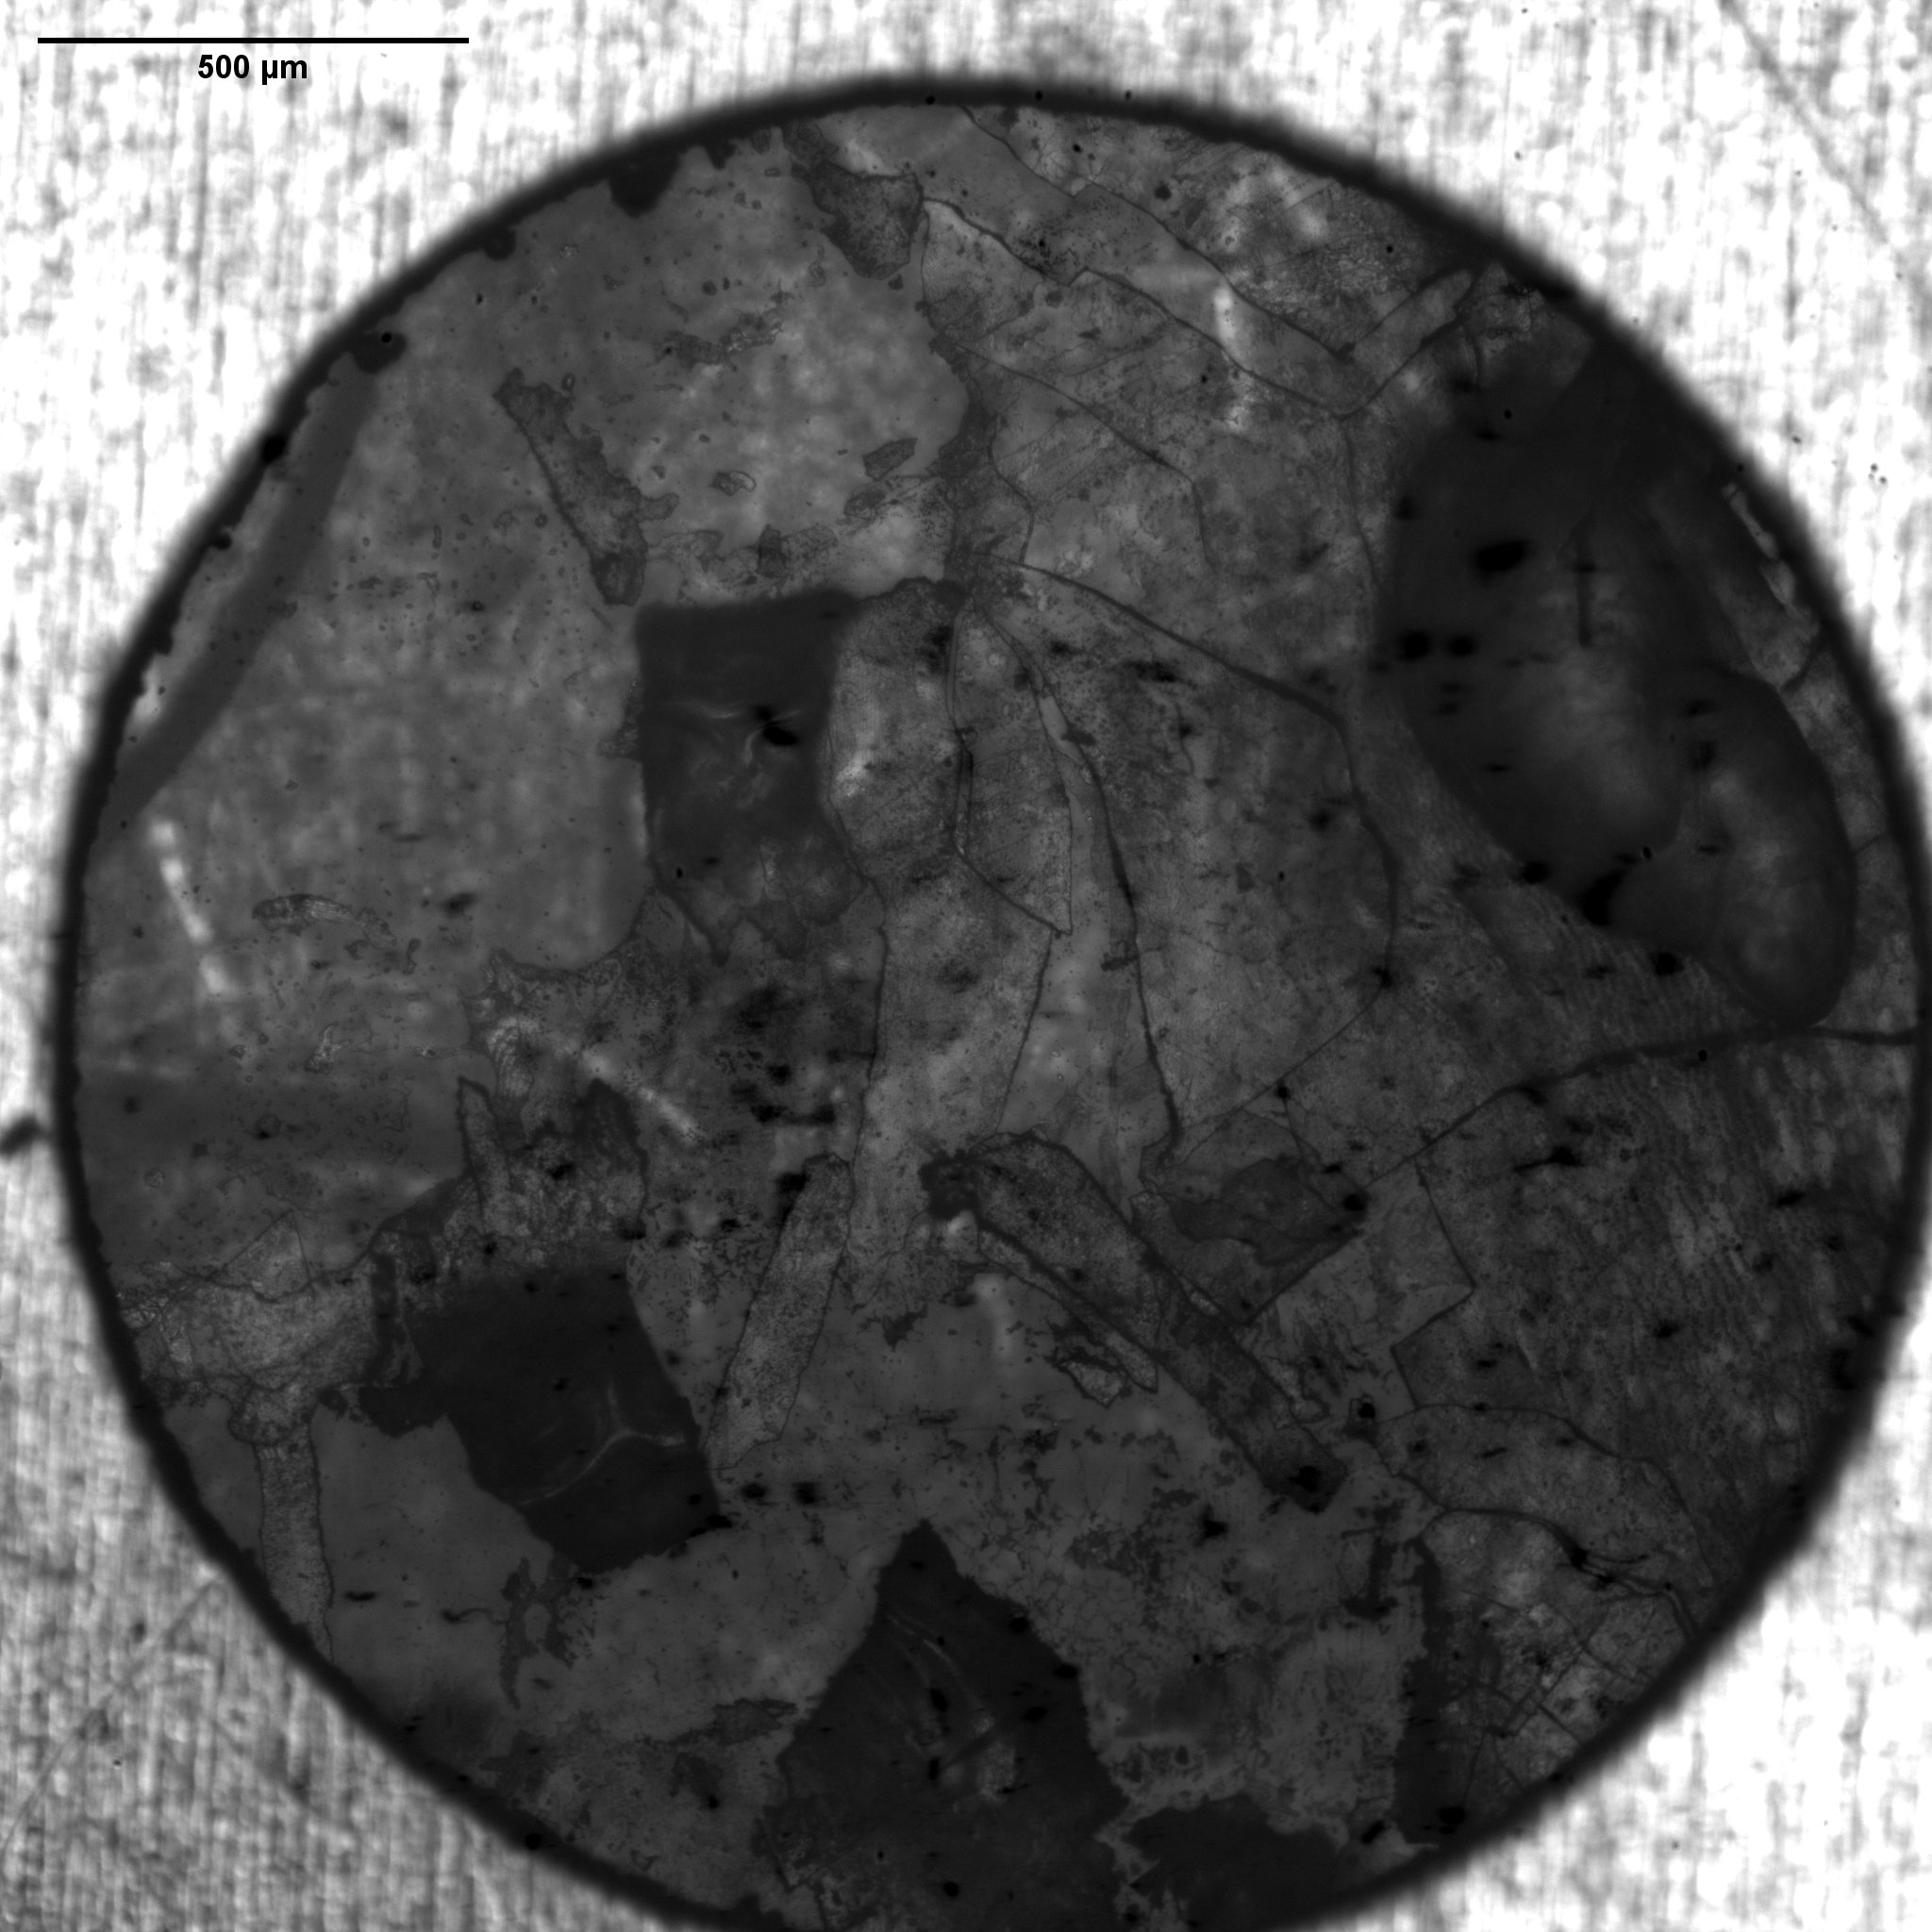
\includegraphics[width=7cm]{Hand freezed Lipid Broken Echtlicht.ome}
		\caption{Sample with a broken ice layer in true light \newline}
	\end{subfigure}
	\begin{subfigure}[]{0.45\textwidth}
		\centering
		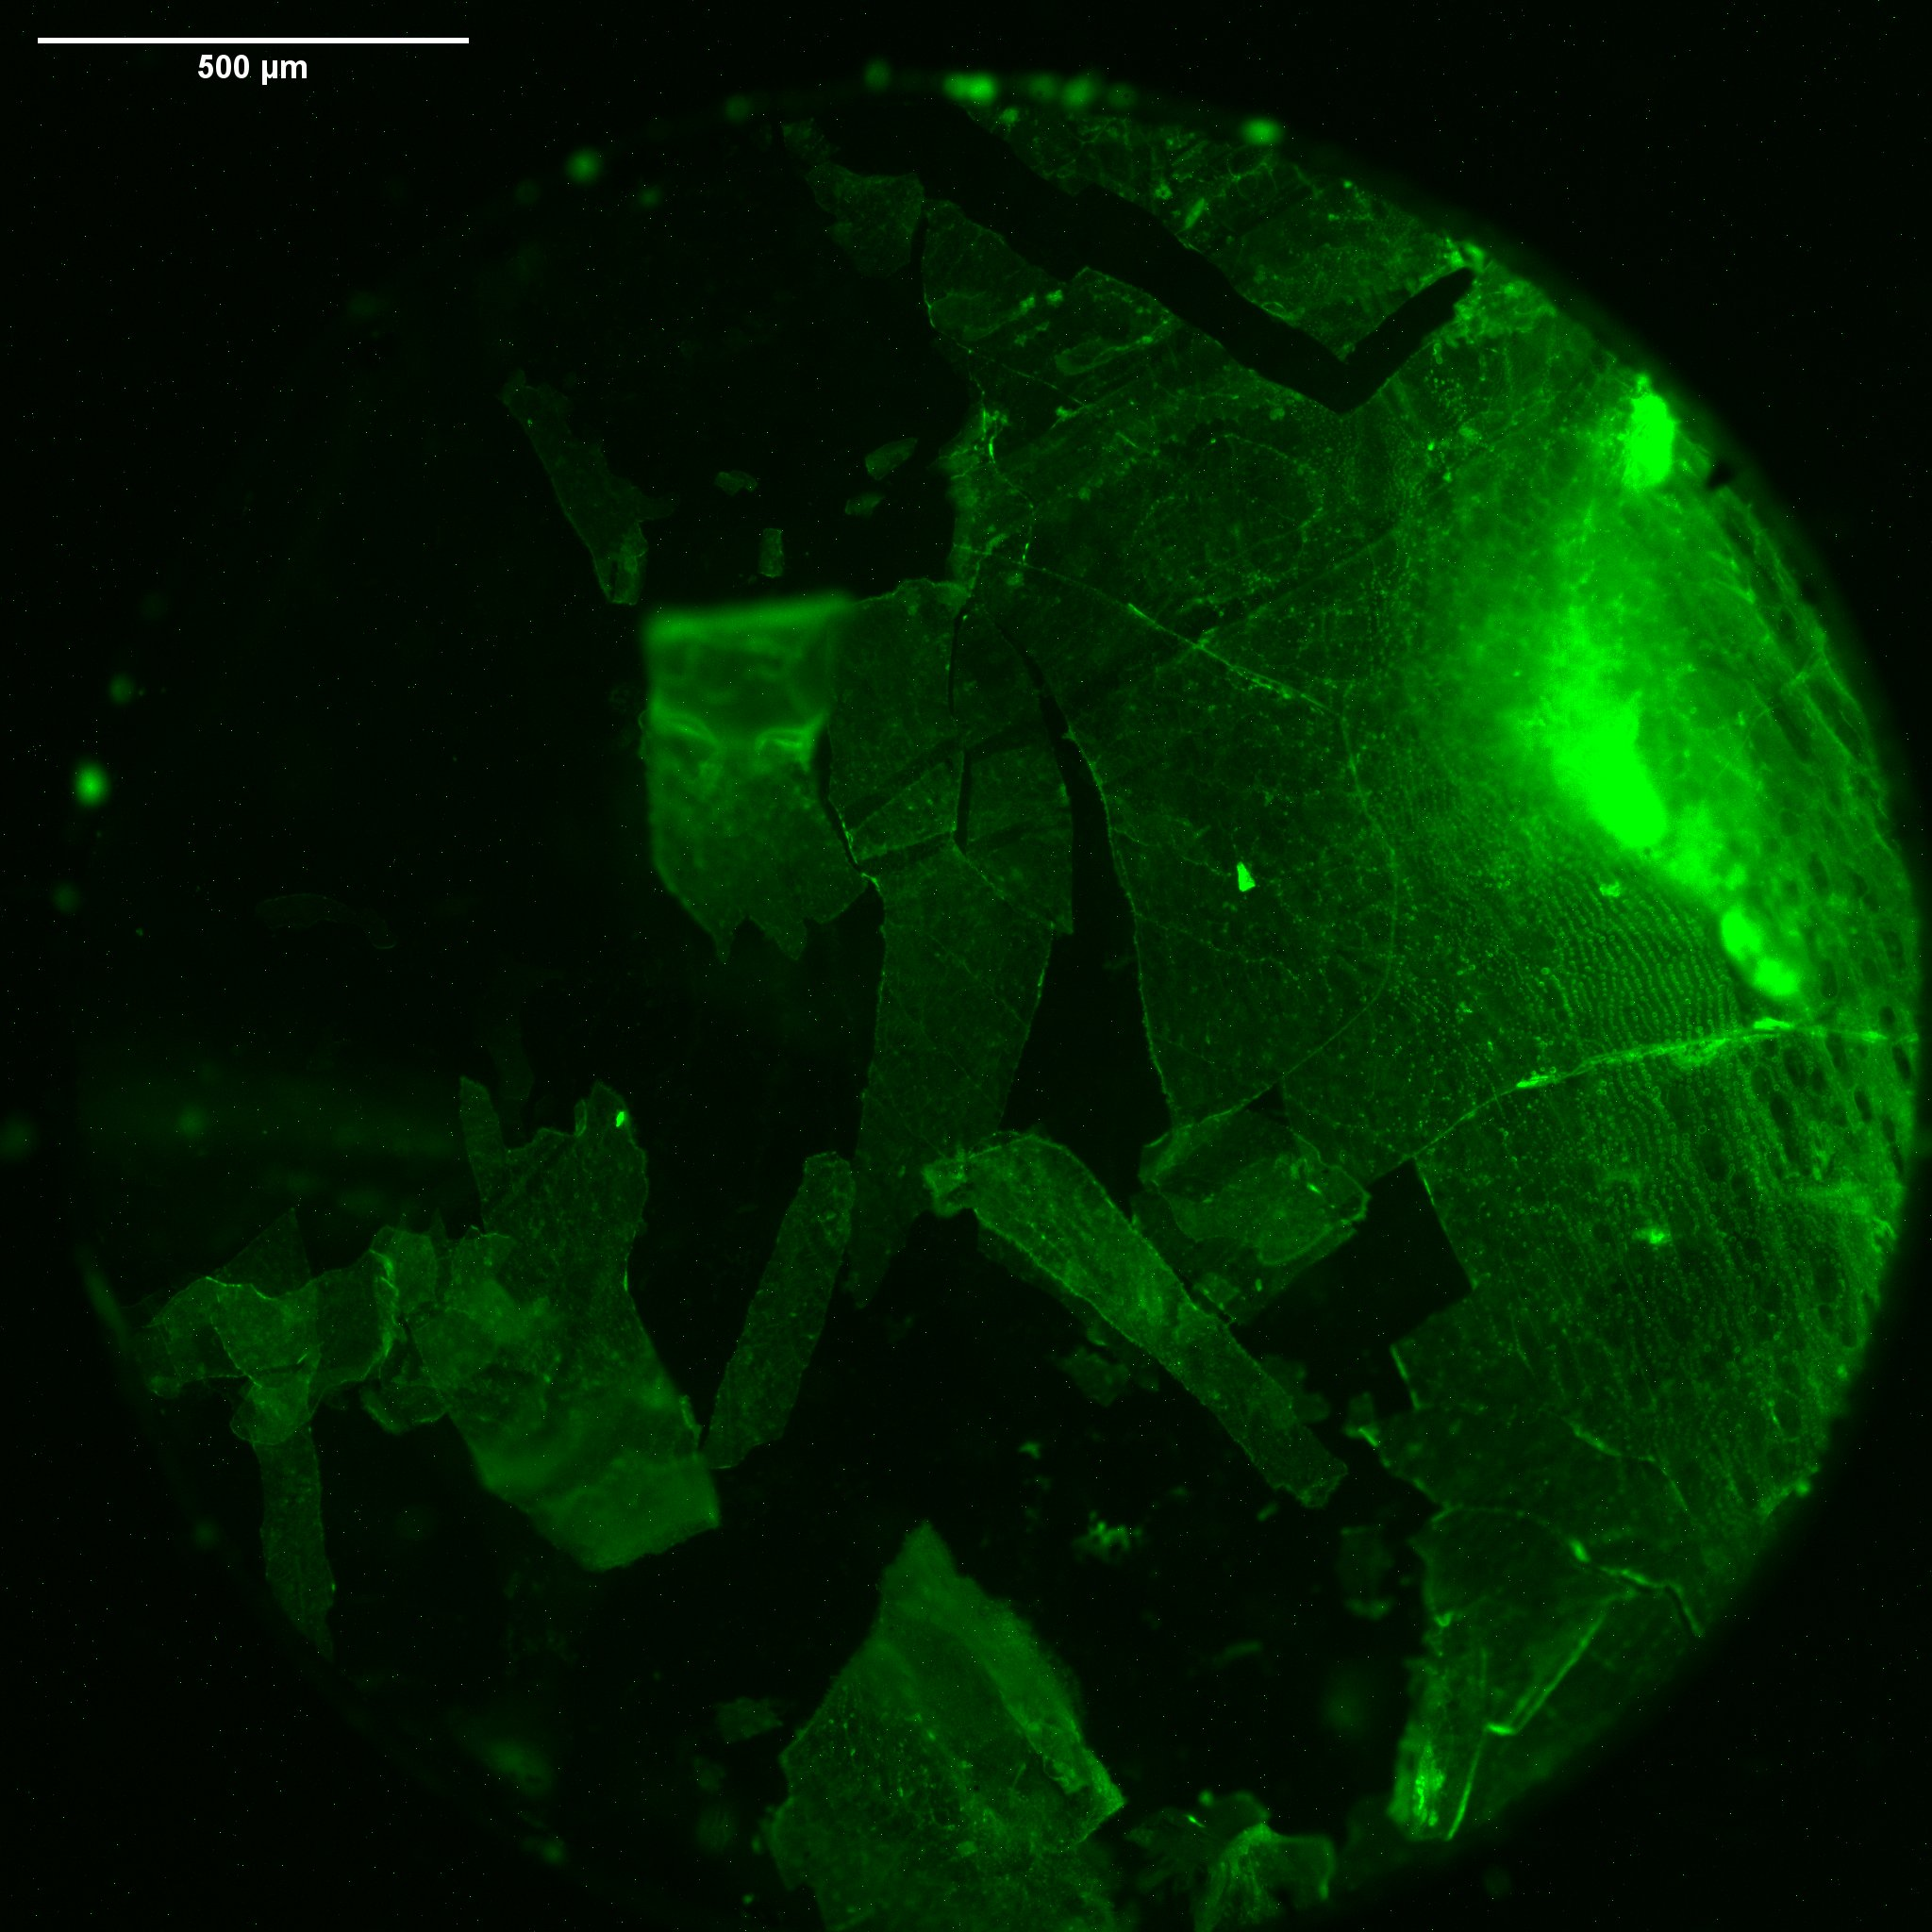
\includegraphics[width=7cm]{Hand freezed Lipid Broken Fluorescence.ome}
		\caption{Sample with a broken ice layer with fluorescence filter}
	\end{subfigure}
	\begin{subfigure}[]{0.45\textwidth}
		\centering
		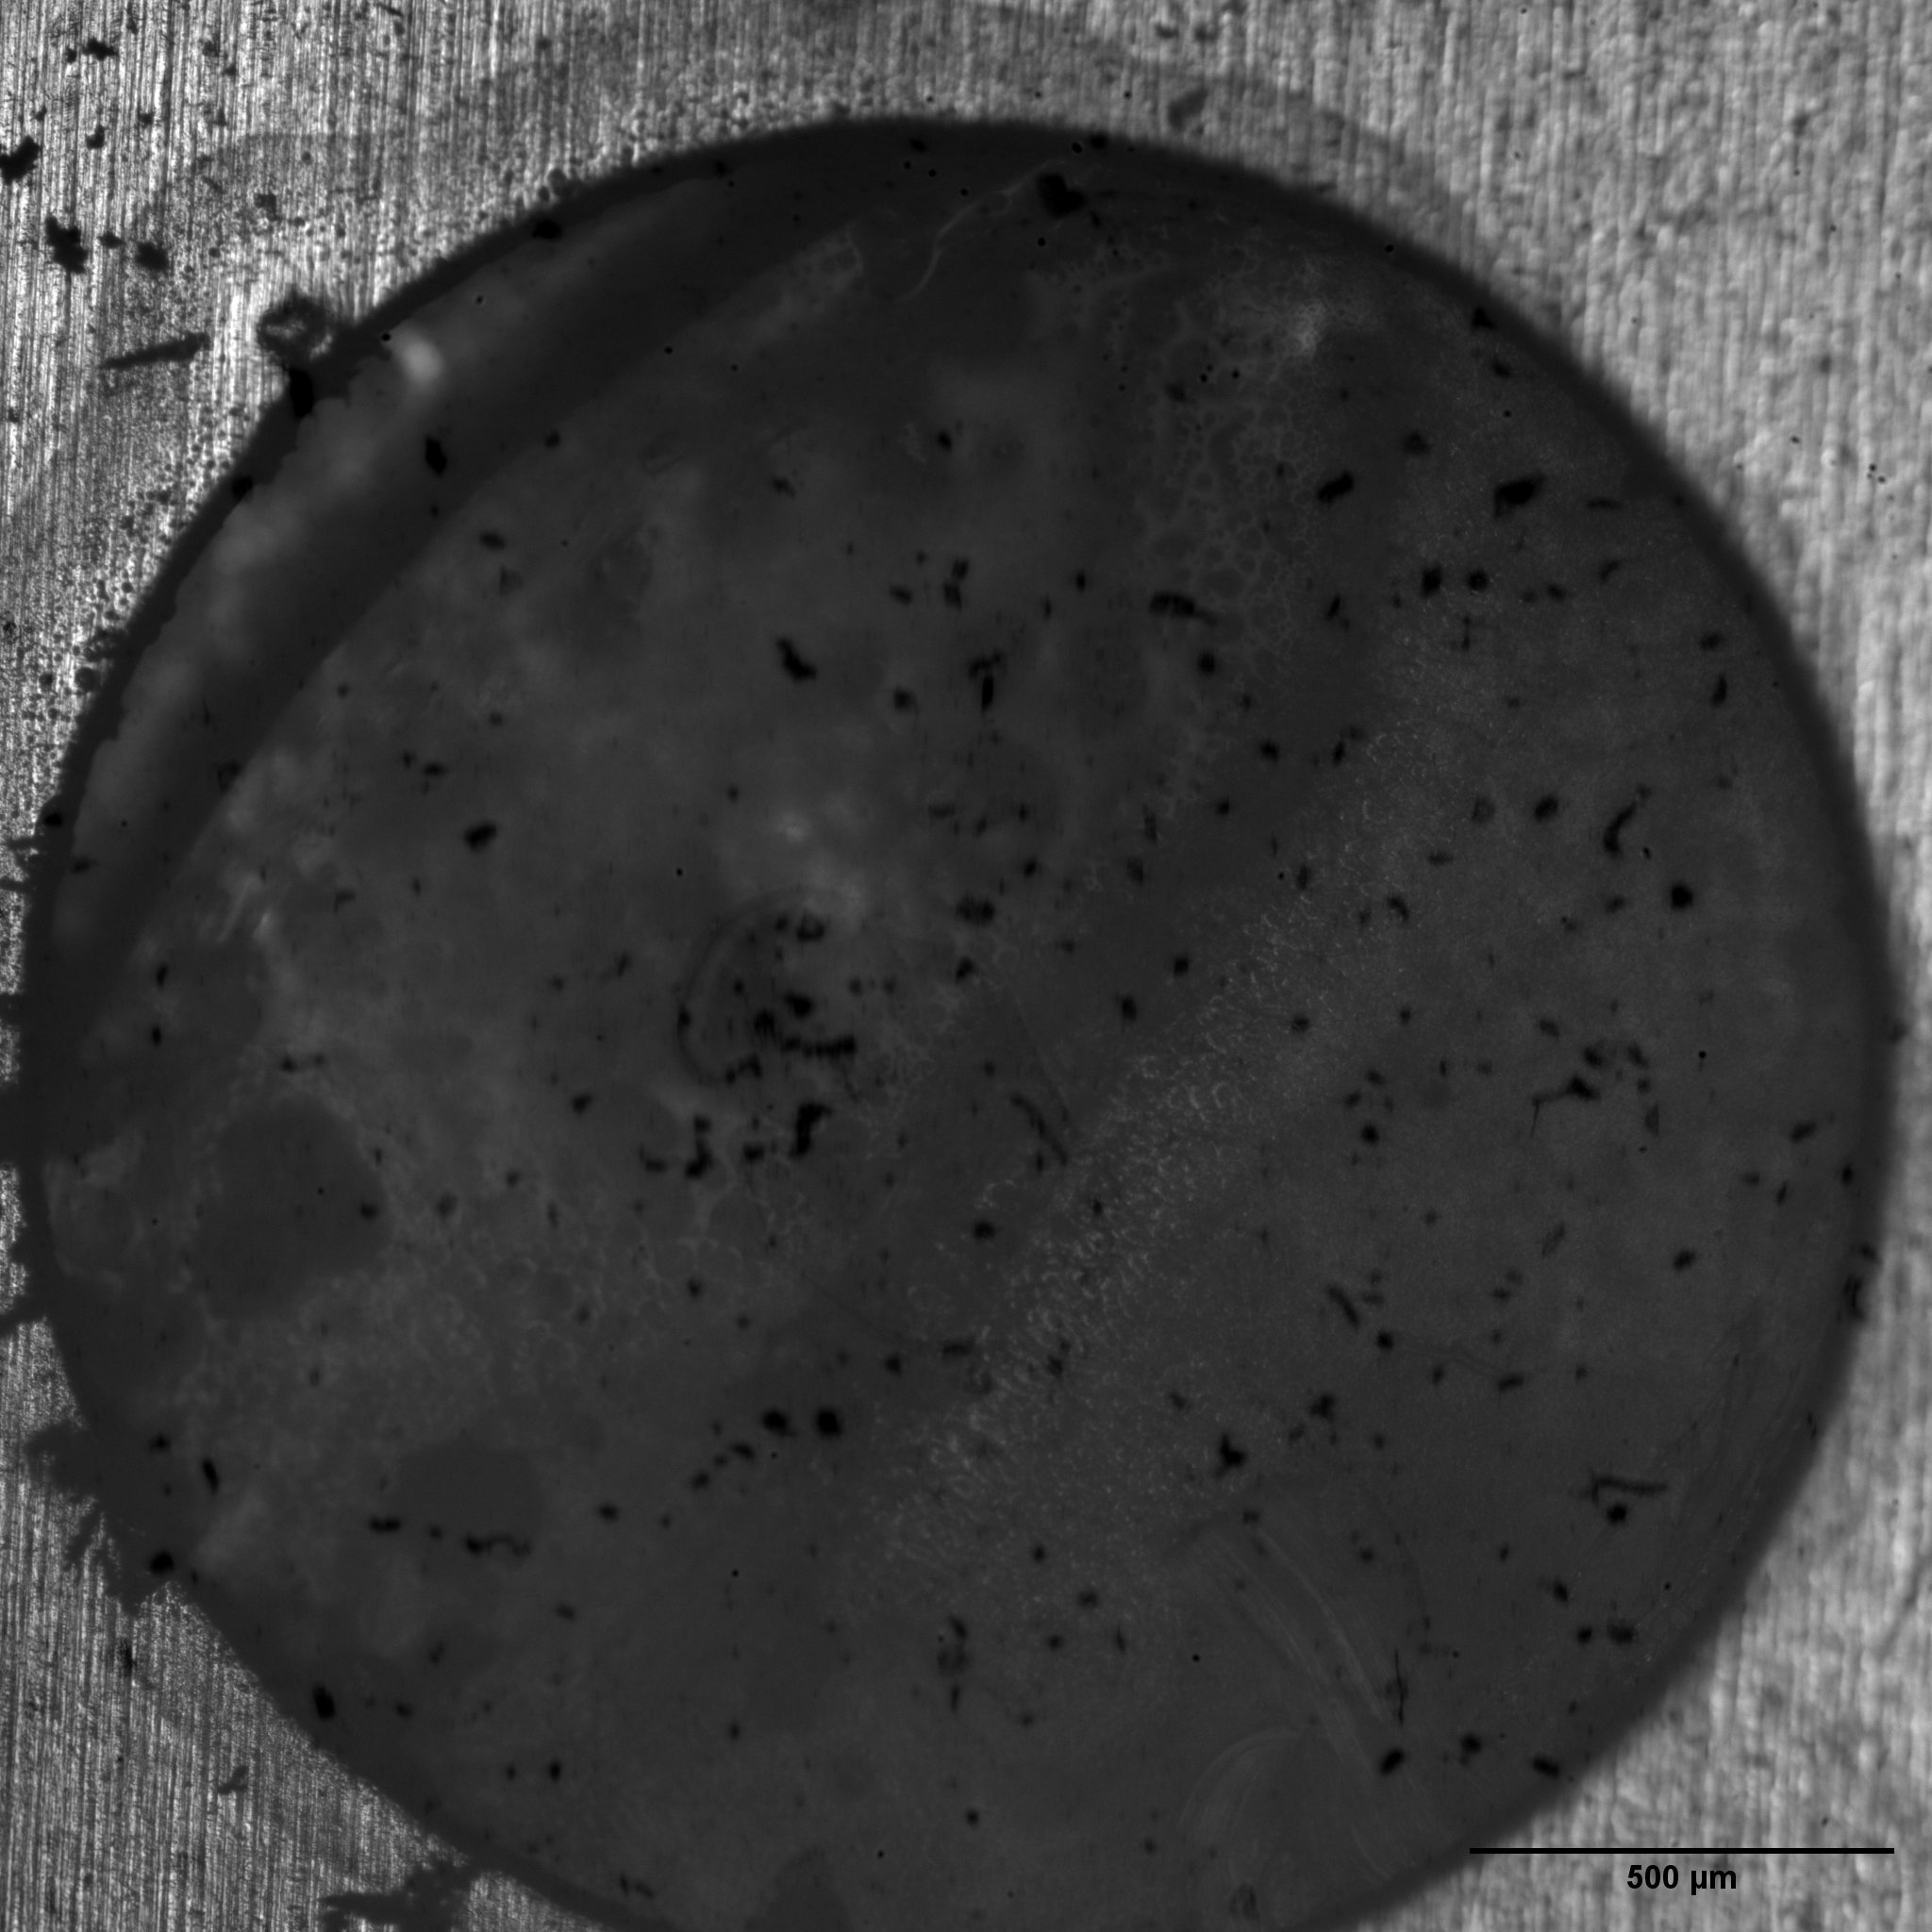
\includegraphics[width=7cm]{Hand freezed Lipid Continuous Echtlicht.ome}
		\caption{Sample with continuous ice layer in true light \newline}
	\end{subfigure}
	\begin{subfigure}[]{0.45\textwidth}
		\centering
		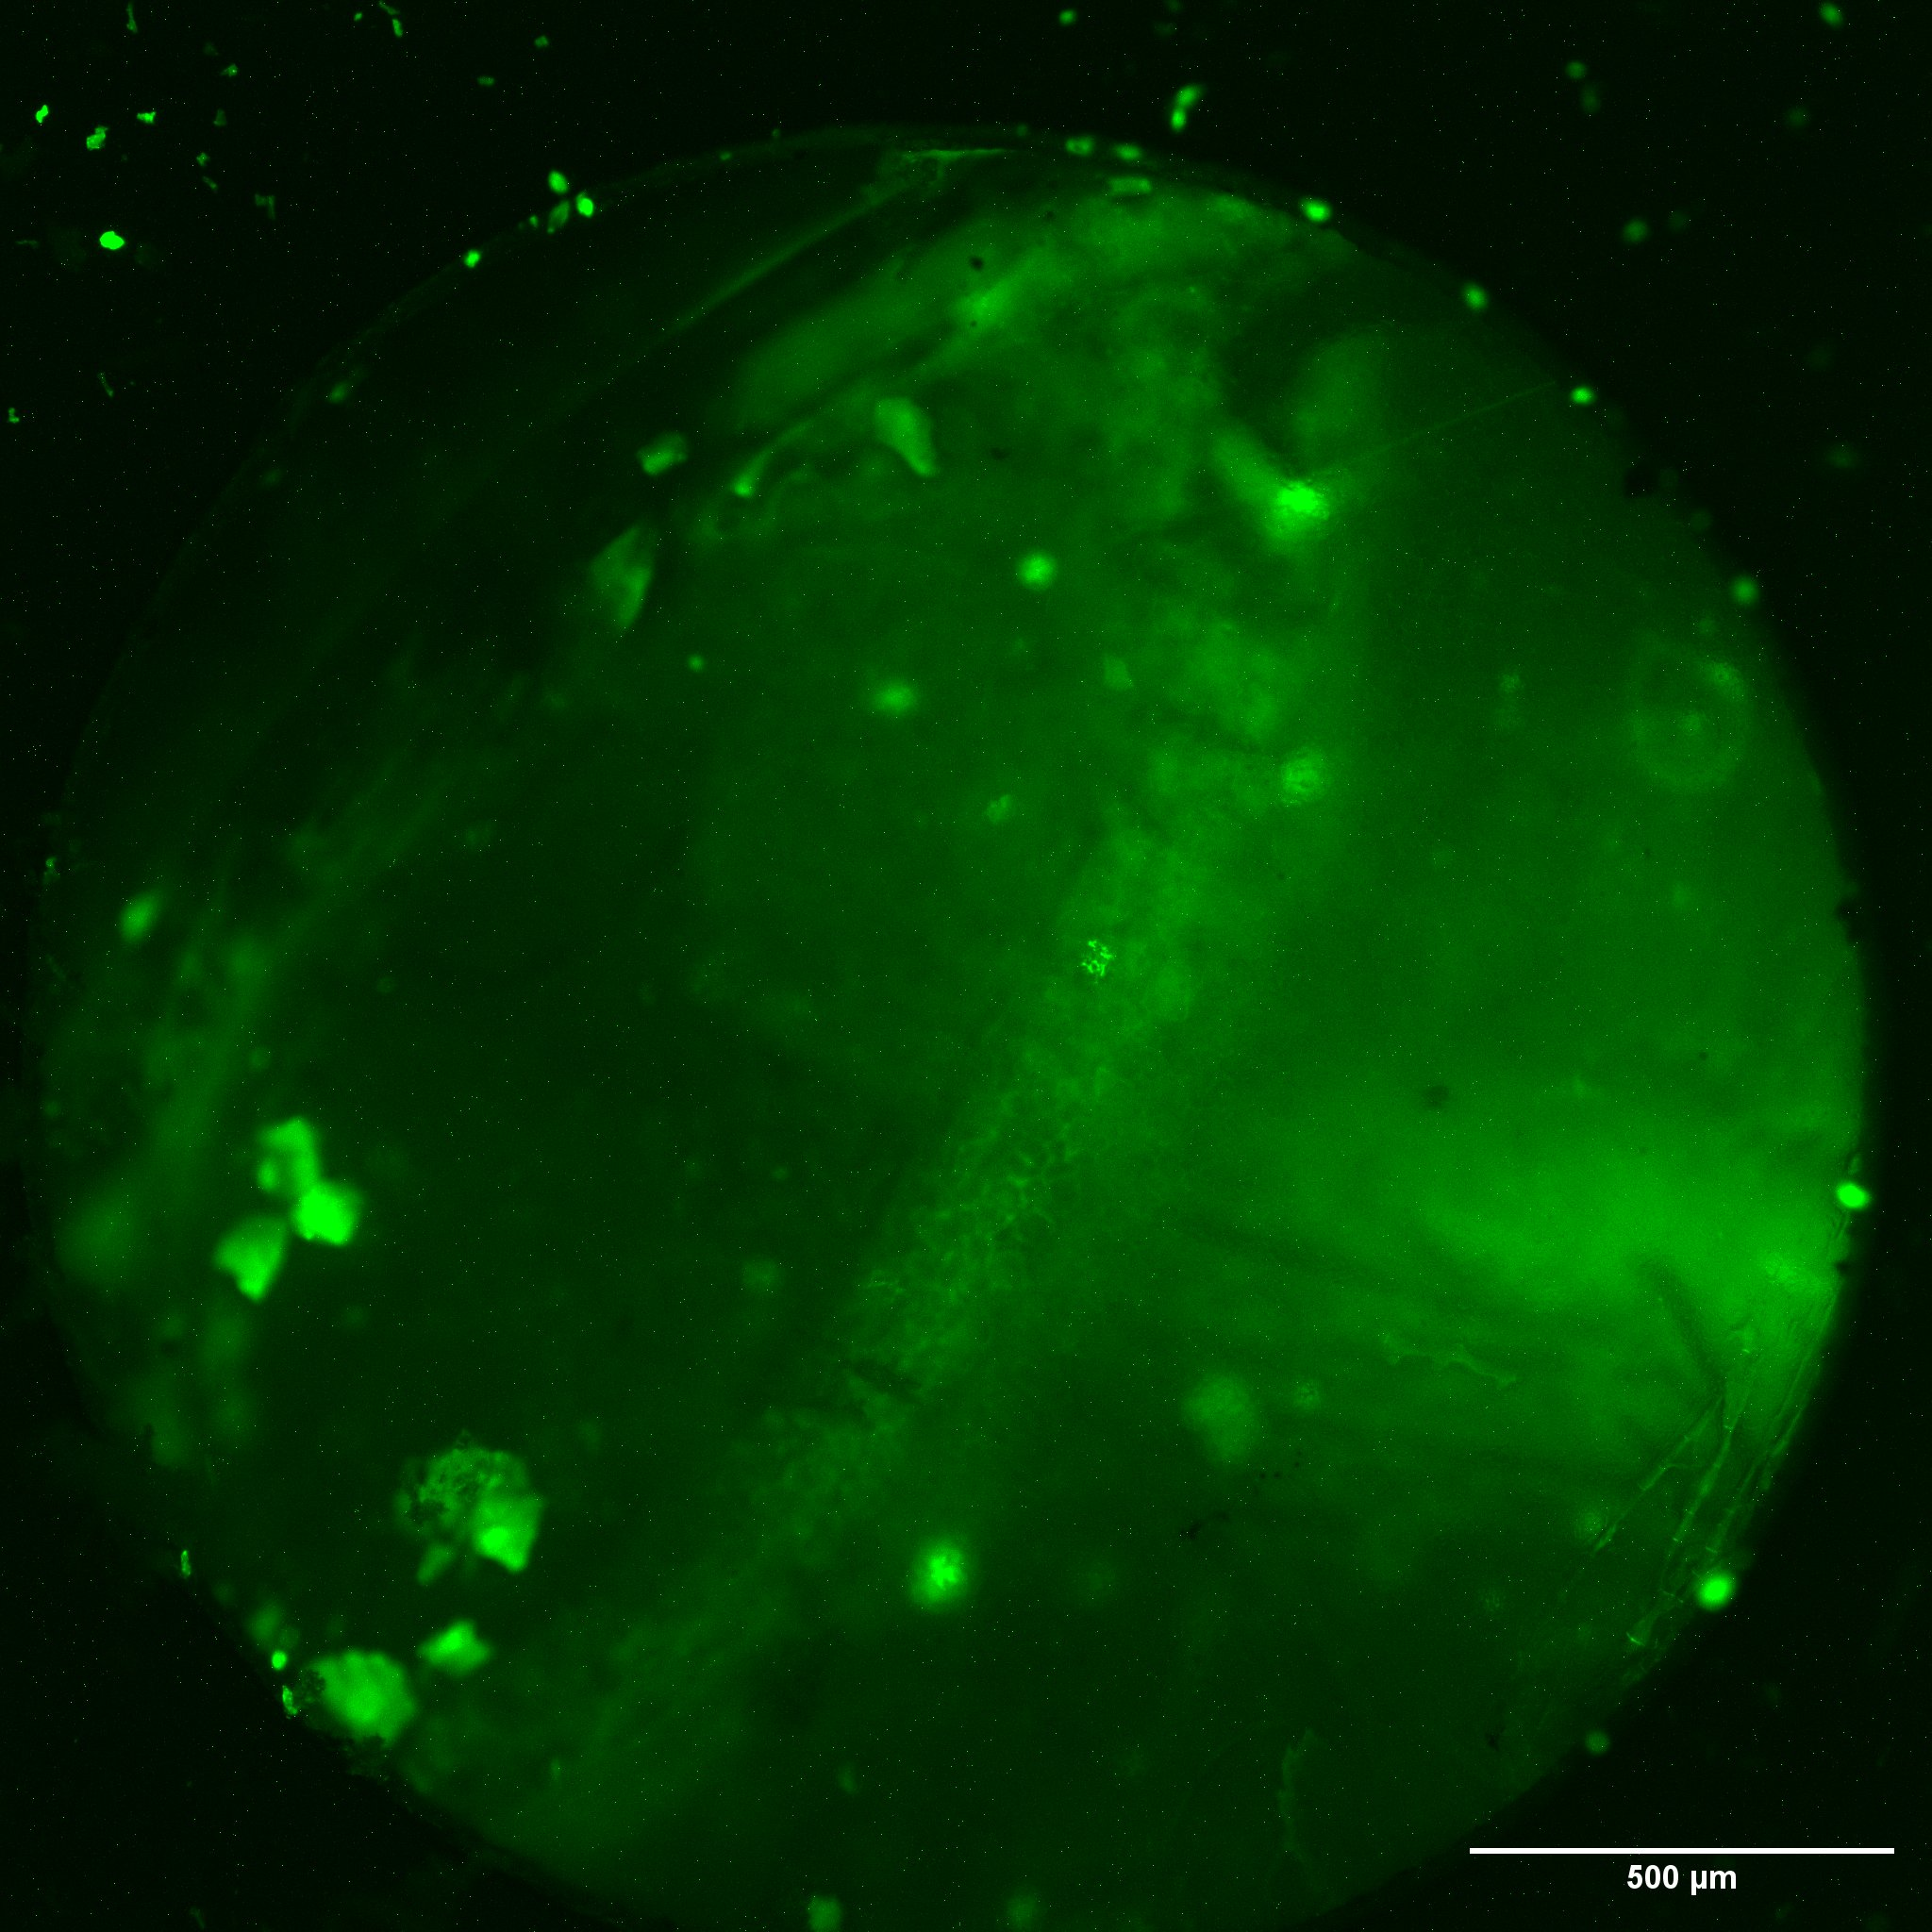
\includegraphics[width=7cm]{Hand freezed Lipid Continuous Fluorescence.ome}
		\caption{Sample with continuous ice layer with fluorescence filter}
	\end{subfigure}
	\caption{Two different examples for hand freezed ice layers on samples. }
	\label{fig:VglHandFreeze}
\end{figure}

\begin{figure}[hbt!]
	\centering
	\begin{subfigure}[]{0.45\textwidth}
		\centering
		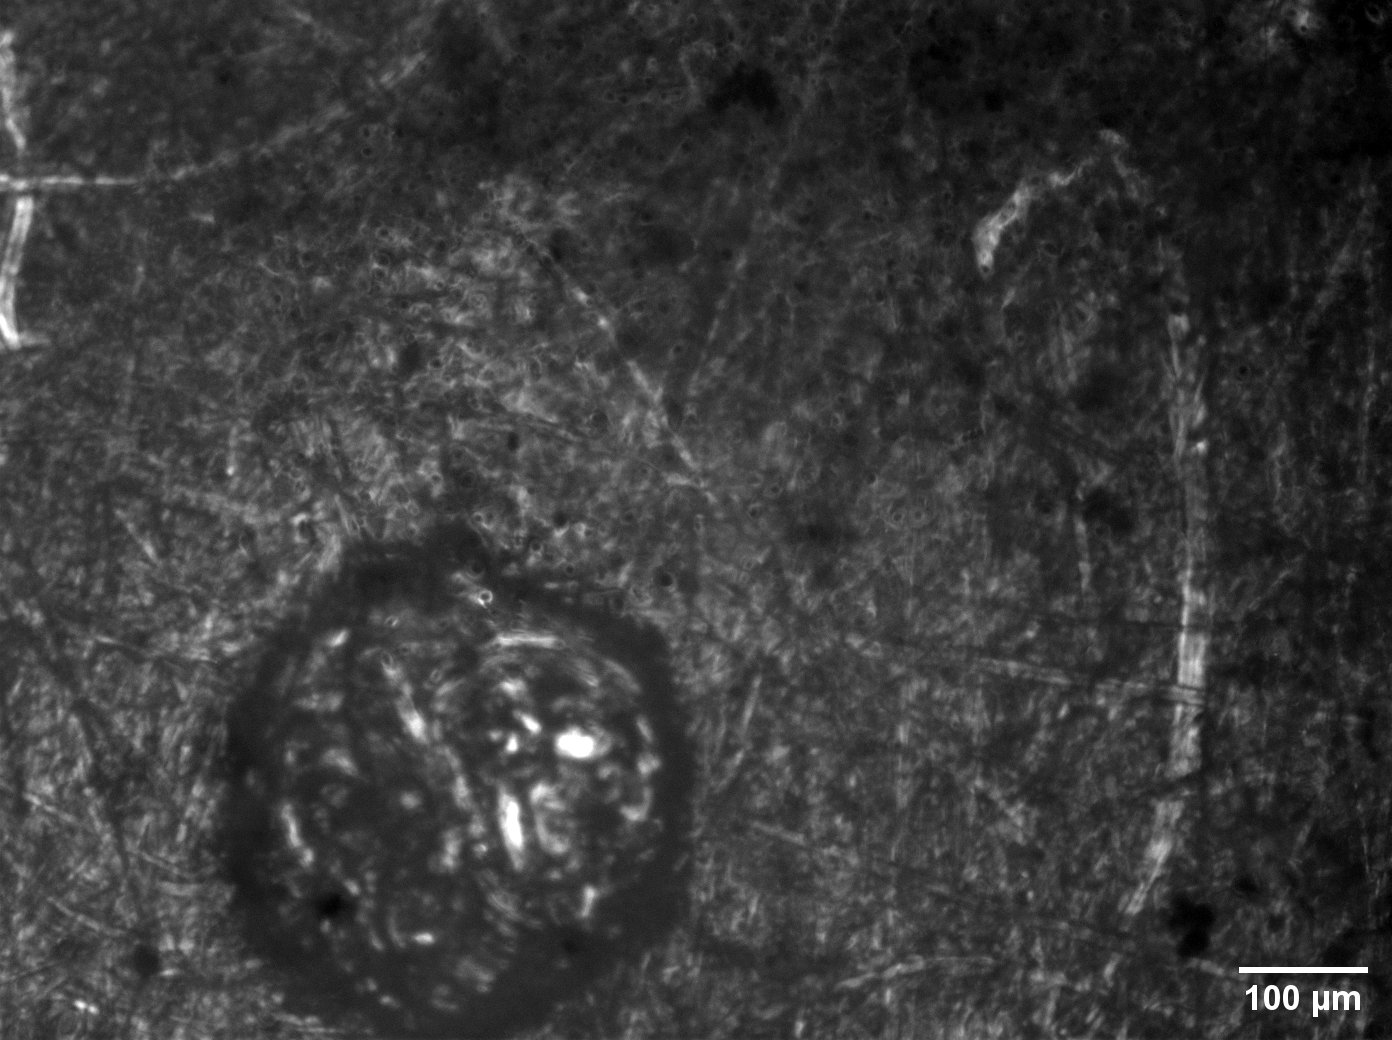
\includegraphics[width=7cm]{Thin Layer Plungefreezer Echtlicht.ome}
		\caption{Sample with thin continuous ice layer in true light \newline}
	\end{subfigure}
	\begin{subfigure}[]{0.45\textwidth}
		\centering
		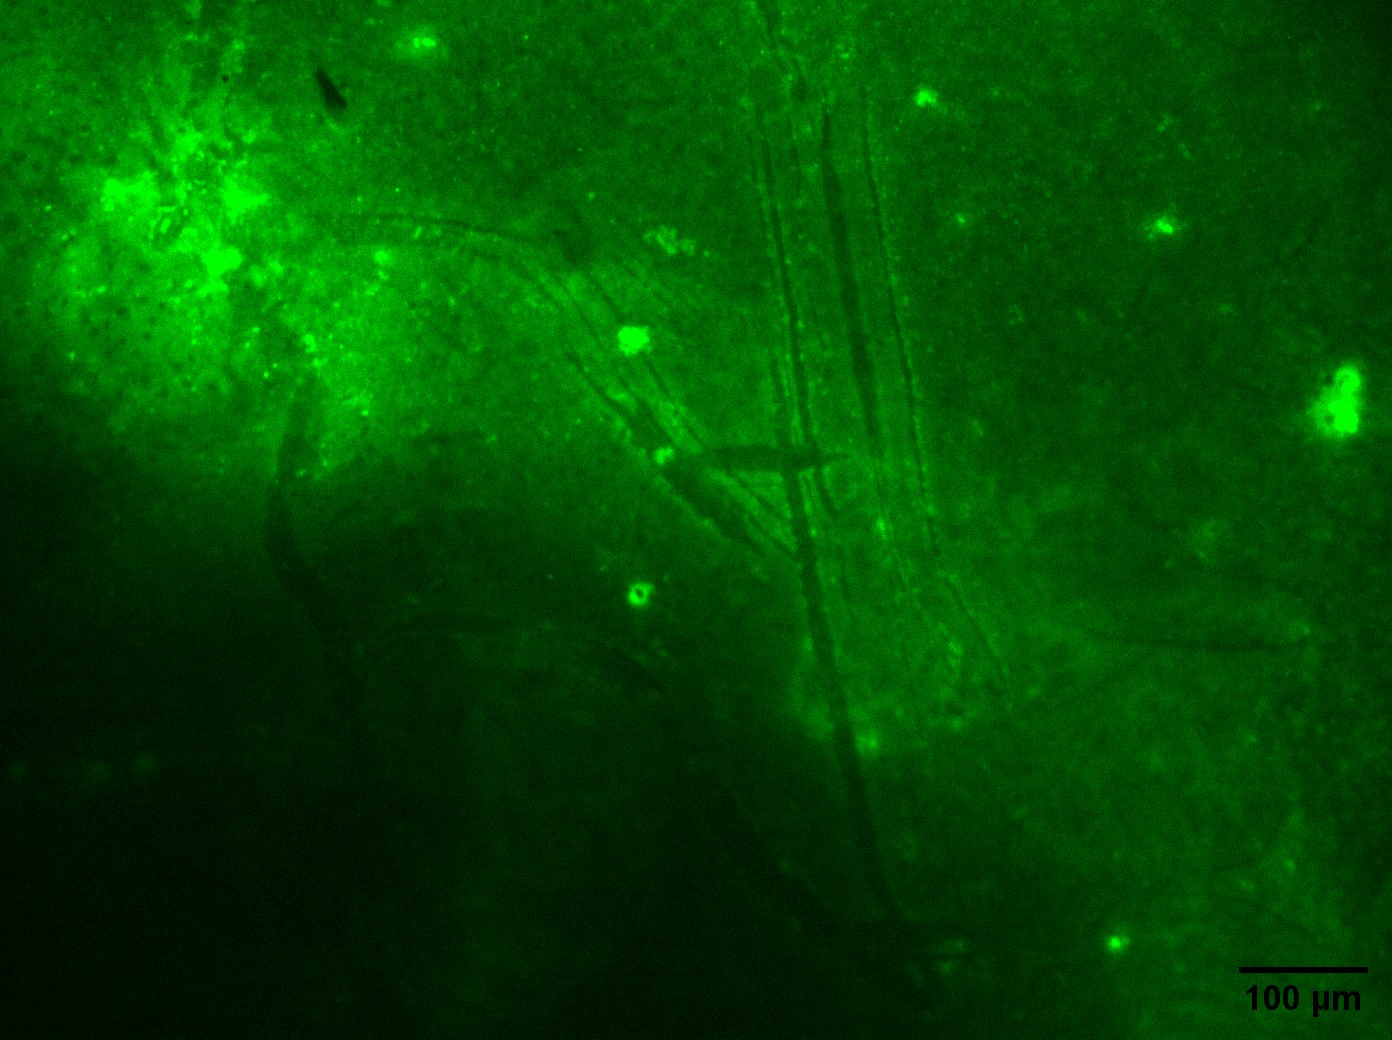
\includegraphics[width=7cm]{Thin Layer Plungefreezer Fluorescence.ome}
		\caption{Sample with thin continuous ice layer with fluorescence filter}
	\end{subfigure}
	\begin{subfigure}[]{0.45\textwidth}
		\centering
		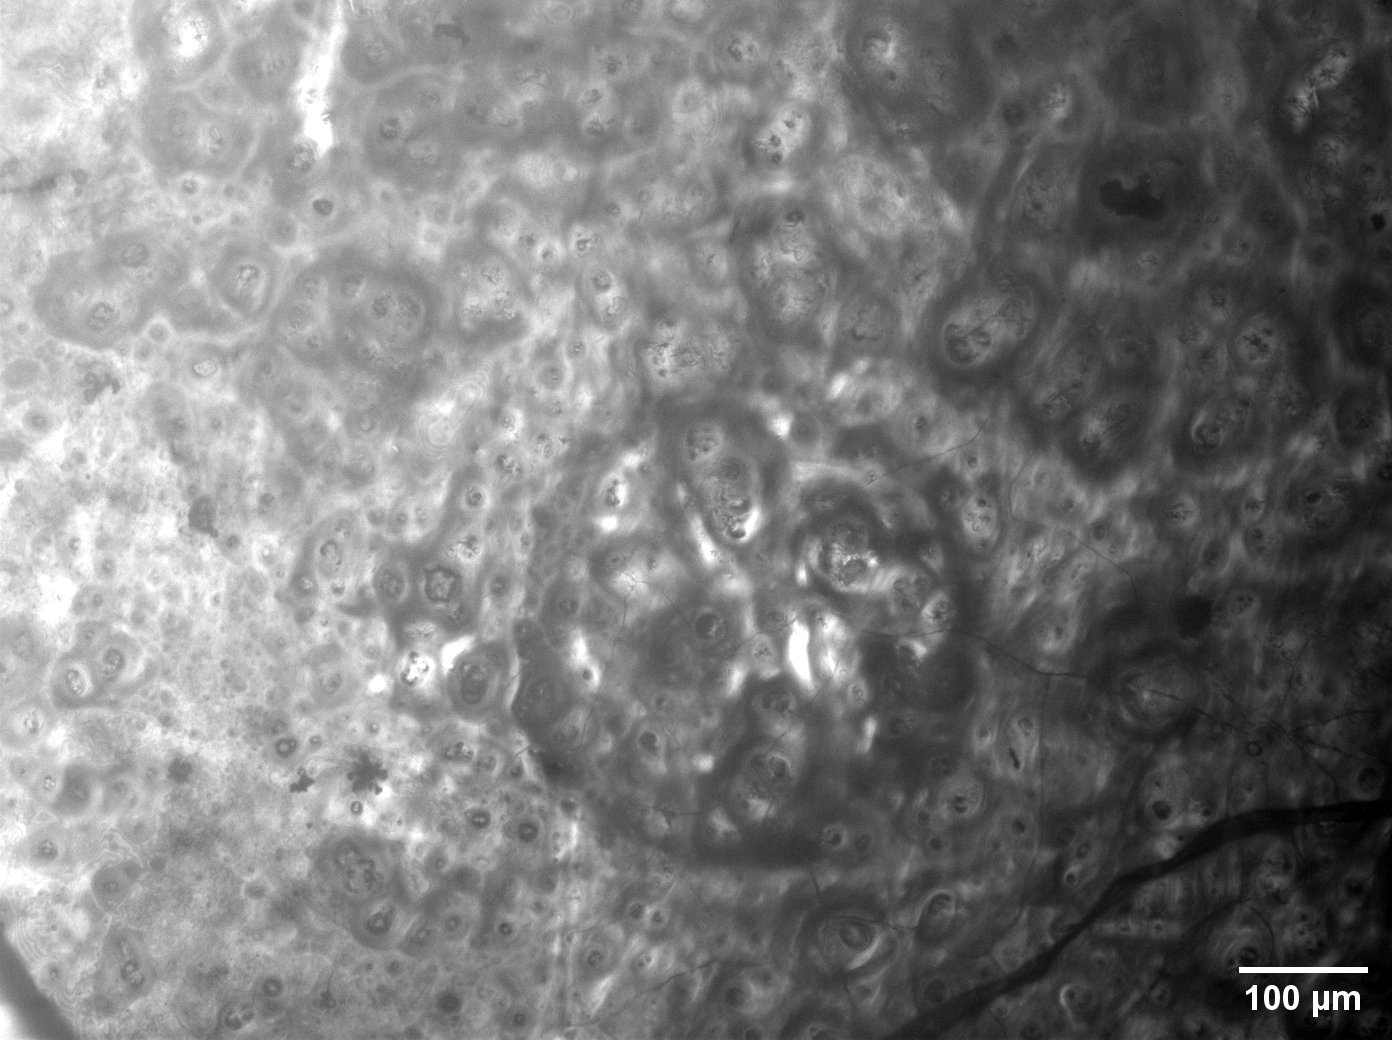
\includegraphics[width=7cm]{Thick Layer Plungefreezer Echtlicht.ome}
		\caption{Sample with thick continuous ice layer in true light with air bubbles}
	\end{subfigure}
	\begin{subfigure}[]{0.45\textwidth}
		\centering
		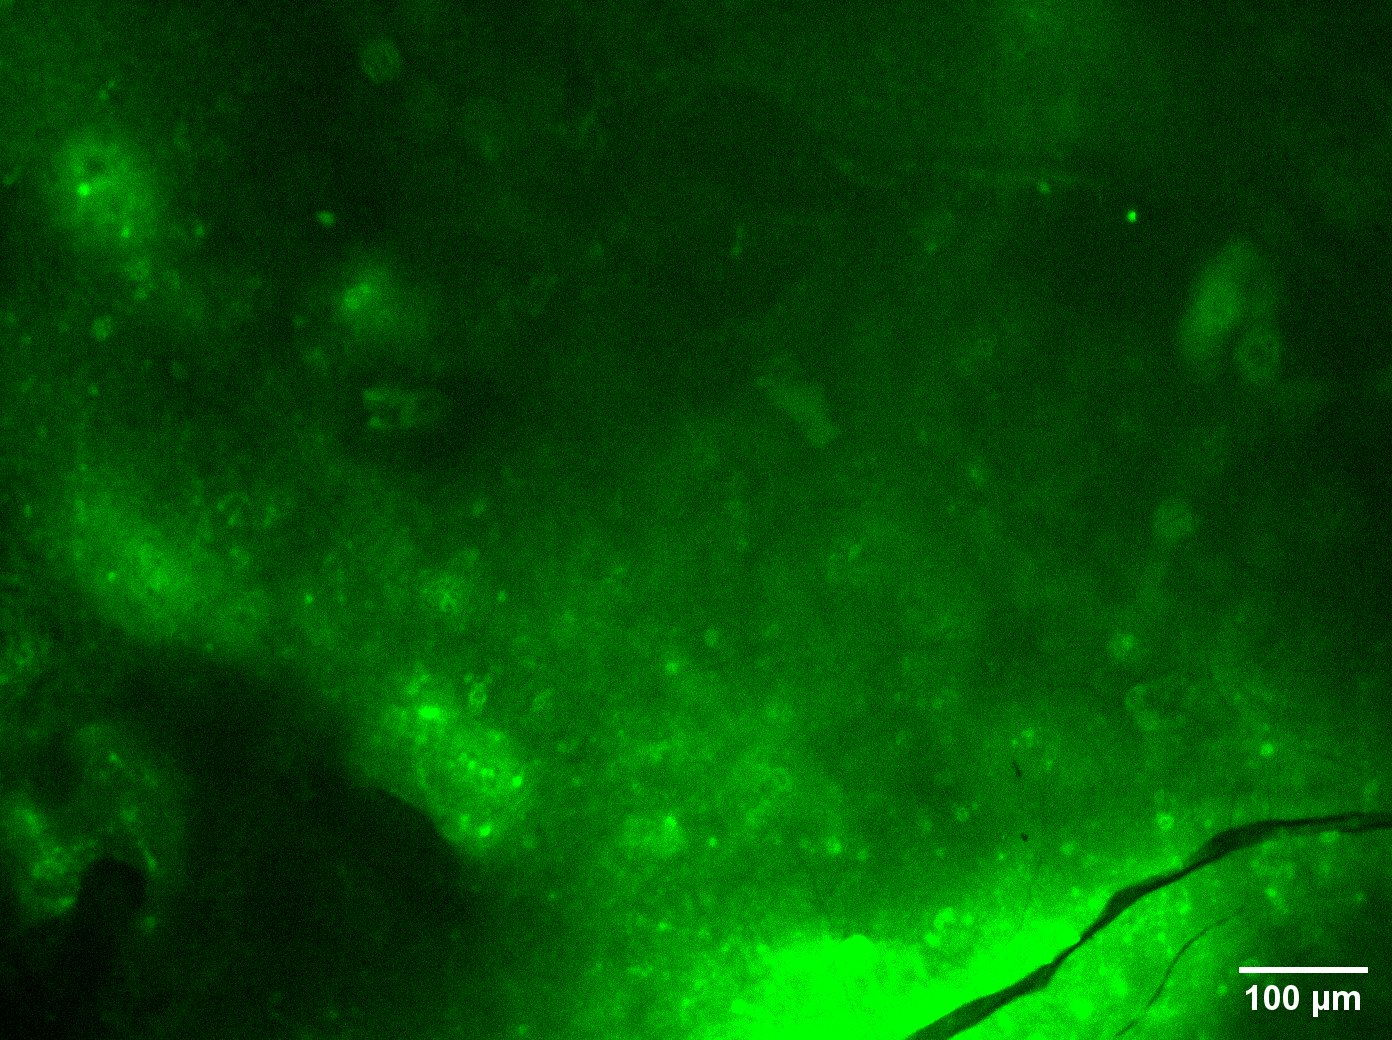
\includegraphics[width=7cm]{Thick Layer Plungefreezer Fluorescence.ome}
		\caption{Sample with thick continuous ice layer with fluorescence filter with air bubbles}
	\end{subfigure}
	\caption{Two different examples for hand freezed ice layers on samples. }
	\label{fig:VglMachineFreeze}
\end{figure}

To further compare both methods, 4 of each hand freezed and plunge freezed samples are compared regarding detachability. The "finger" is attached with HFE onto the sample. With movement up on the Z axis, the "finger" is inducing tensile force to the ice layer as an attempt to detach an ice piece. The results are categorized in 4 categories: Not successful pulls don't have visible changes of the flourescent ice layer, Partially successes are visible breaks or clear movement of ice parts on the ice layer, Successful liftoff is a missing piece and a visible piece on the finger, which could be used for future steps.

In the results, there is no difference between hand-freezed and plunge-freezed samples regarding detachability (Fig. \ref{table:AttemptsHandsvsMachine}). Therefore, using a plunge-freezer does not result in samples with favorable properties.

\begin{table}
	\centering
	\begin{tabular}{|c|c|c|}
		\hline
		Category & Hand-freezed & Plunge-freezed \\
		\hline
		\hline
		count executed tries & 4 & 4\\
		\hline
		unsuccessful & 3 & 3\\
		\hline
		breaks/movement of ice & 1 & 1\\
		\hline
		piece lifted with finger & 0 & 0\\
		\hline		
	\end{tabular}
	\caption{Comparison of detachability between hand-freezed and plunge-freezed samples}
	\label{table:AttemptsHandsvsMachine}
\end{table}

Additonally, two other PDMS mixtures are used. 4:1 with \SI{10}{\minute} and $100\,\%$ plasma activation is used as reference. 50:1 mixture ratio is additionally used with different plasma activation duration. To verify the results of \cite{Ohishi.2017}, PDMS with 50:1 mixture treated with \SI{3}{\minute} at each $25\,\%$ and $100\,\%$ and \SI{10}{\minute} at $100\,\%$. 

Different PDMS mixture ratio with different plasma activations are tested at cryogenic temperatures. With previous setup, plasma activation of 1:2 mixture ratio PDMS resulted into a more stable layer with more adhesion. Also 50:1 is tested with high plasma activation. The tensile stress of 50:1 mixture ratio is \SI{60}{\kilo\pascal} \cite{IbanezIbanez.2022}.  \cite{Ohishi.2017} suggests that strong plasma activation over \SI{3}{\minute} results of a decrease of adhesion strength of around$90\,\%$. Additionally, 4:1 mixture ratio with high plasma activation is tested.

%TODO vielleicht noch in state of the art???? 
PDMS properties are also temperature dependent. In \cite{Zhang.2020}, multiple characteristics are determined for cryogenic temperatures. The PDMS is prepared with the standard mixture ratio of 10:1. The compressive strength increases with lower temperatures until \SI{-123.15}{\degreeCelsius}. At this temperature, the compressive strength reaches a maximum of \SI{224.50}{\mega\pascal} in average. At lower temperatures, the PDMS gets brittle. At \SI{-150.15}{\degreeCelsius} PDMS has a compressive strength of \SI{106.99}{\mega\pascal}.

The "finger" requires a temperature of \SI{-160}{\degreeCelsius}. Therefore, the temperature drops enough to make PDMS of 10:1 mixture ratio brittle. Generally, a brittle PDMS surface helps to detach the ice layer. Tensile forces loosens the PDMS under the Ice. The PDMS layer breaks within itself, loosening the ice layer from the rest of the sample. Still, an extreme brittleness is needed, which may not be reached. With PDMS of other mixture ratios, the brittleness could change, including the temperature dependency.

To compare PDMS coated slides to lipid coated slides, the same experiment is repeated for three different mixture ratios. Under the microscope, a continuous layer of ice is visible. \ref{fig:VglPDMSicemixtureratio}). The Ice layer has the same structure for each mixture ratio. Still, the ice layer has a different structure to ice frozen on lipid slides (fig \ref{fig:VglHandFreeze}, \ref{fig:VglMachineFreeze}). The layer is only interrupted by the imprint of pincers used for plunge freezing, visible in fig. \ref{fig:VglPDMSicemixtureratio_f}. Also almost no cracks are visible in the ice layer. This indicates a strong continuous ice layer.

\begin{figure}[hbt!]
	\centering
	\begin{subfigure}[]{0.45\textwidth}
		\centering
		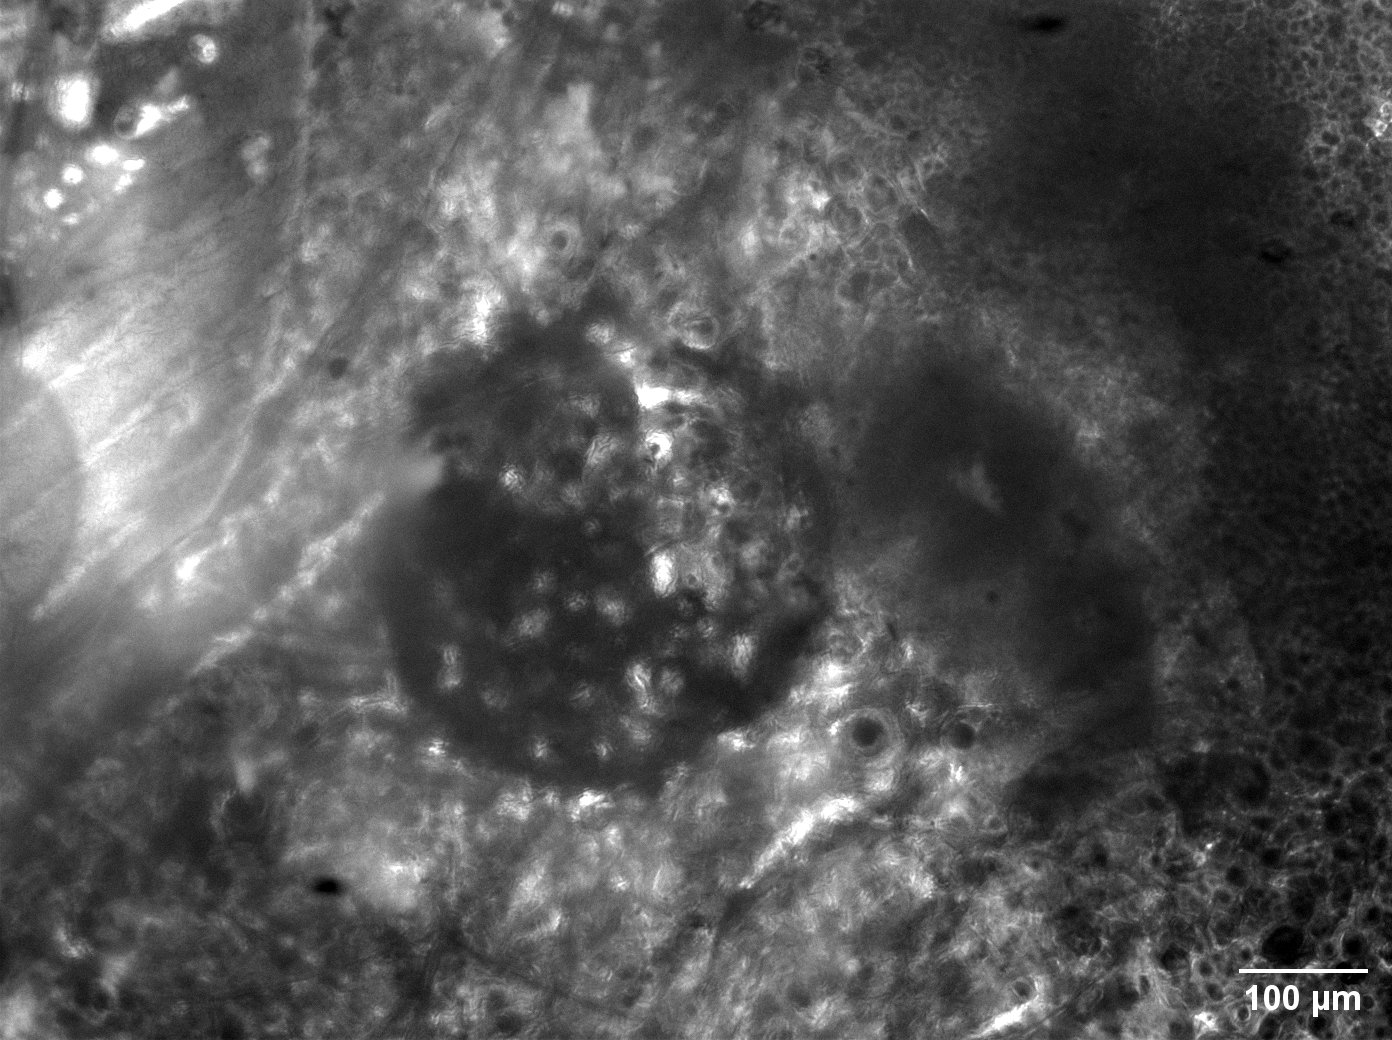
\includegraphics[width=7cm]{1_2_Ice_echtlicht.ome}
		\caption{PDMS 1:2 sample in true light}
	\end{subfigure}
	\begin{subfigure}[]{0.45\textwidth}
		\centering
		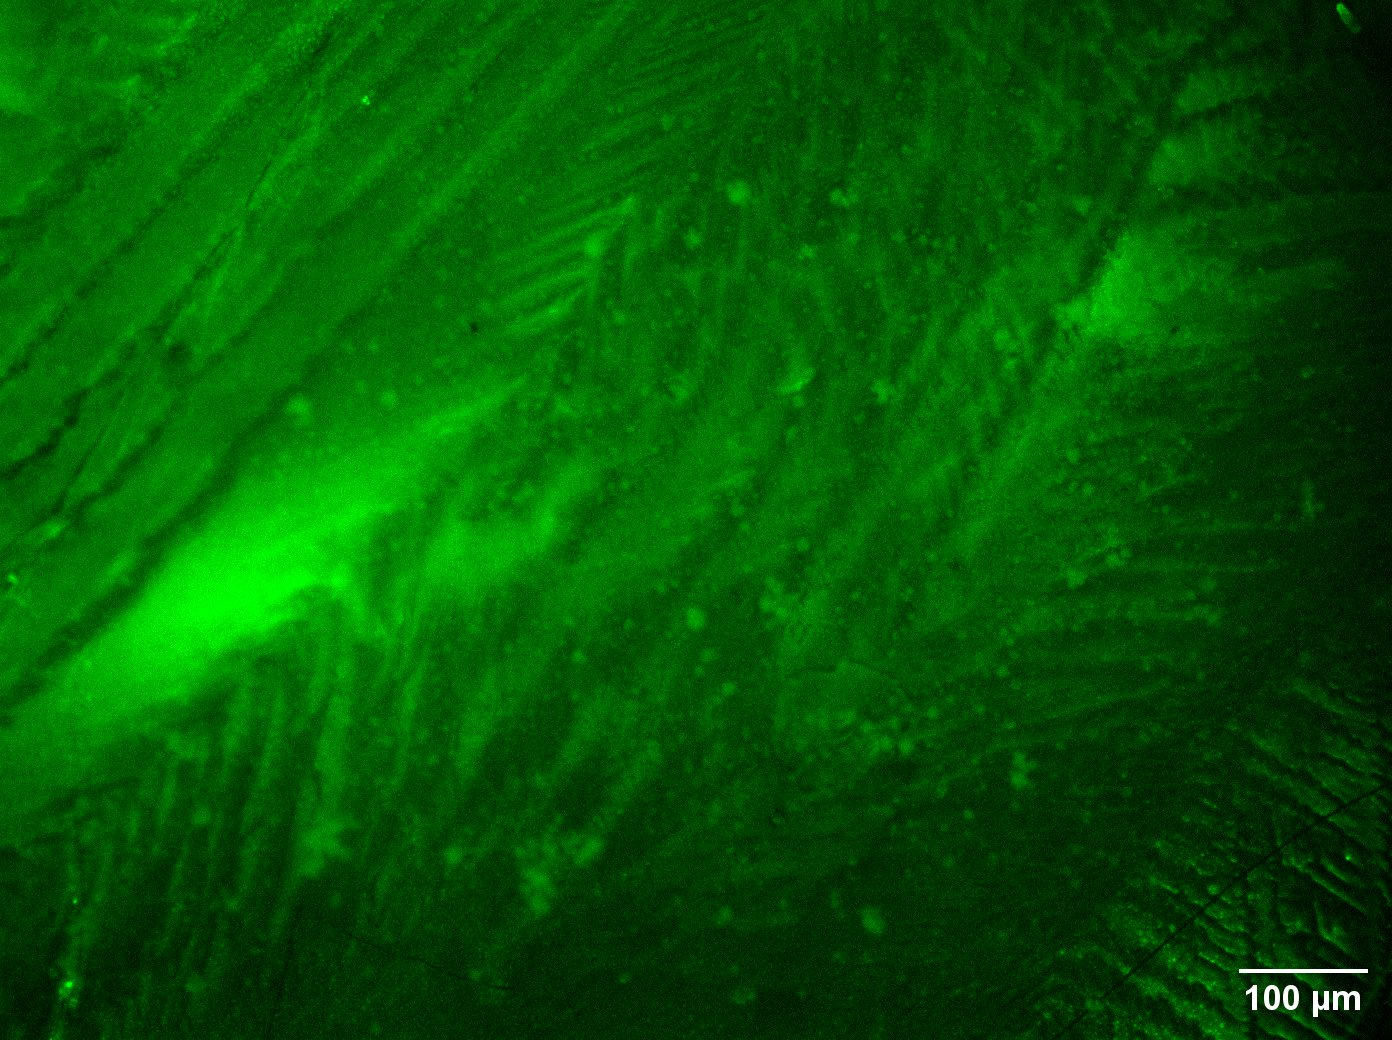
\includegraphics[width=7cm]{1_2_Ice_fluorescence.ome}
		\caption{PDMS 1:2 sample with fluorescence filter}
	\end{subfigure}
	\begin{subfigure}[]{0.45\textwidth}
		\centering
		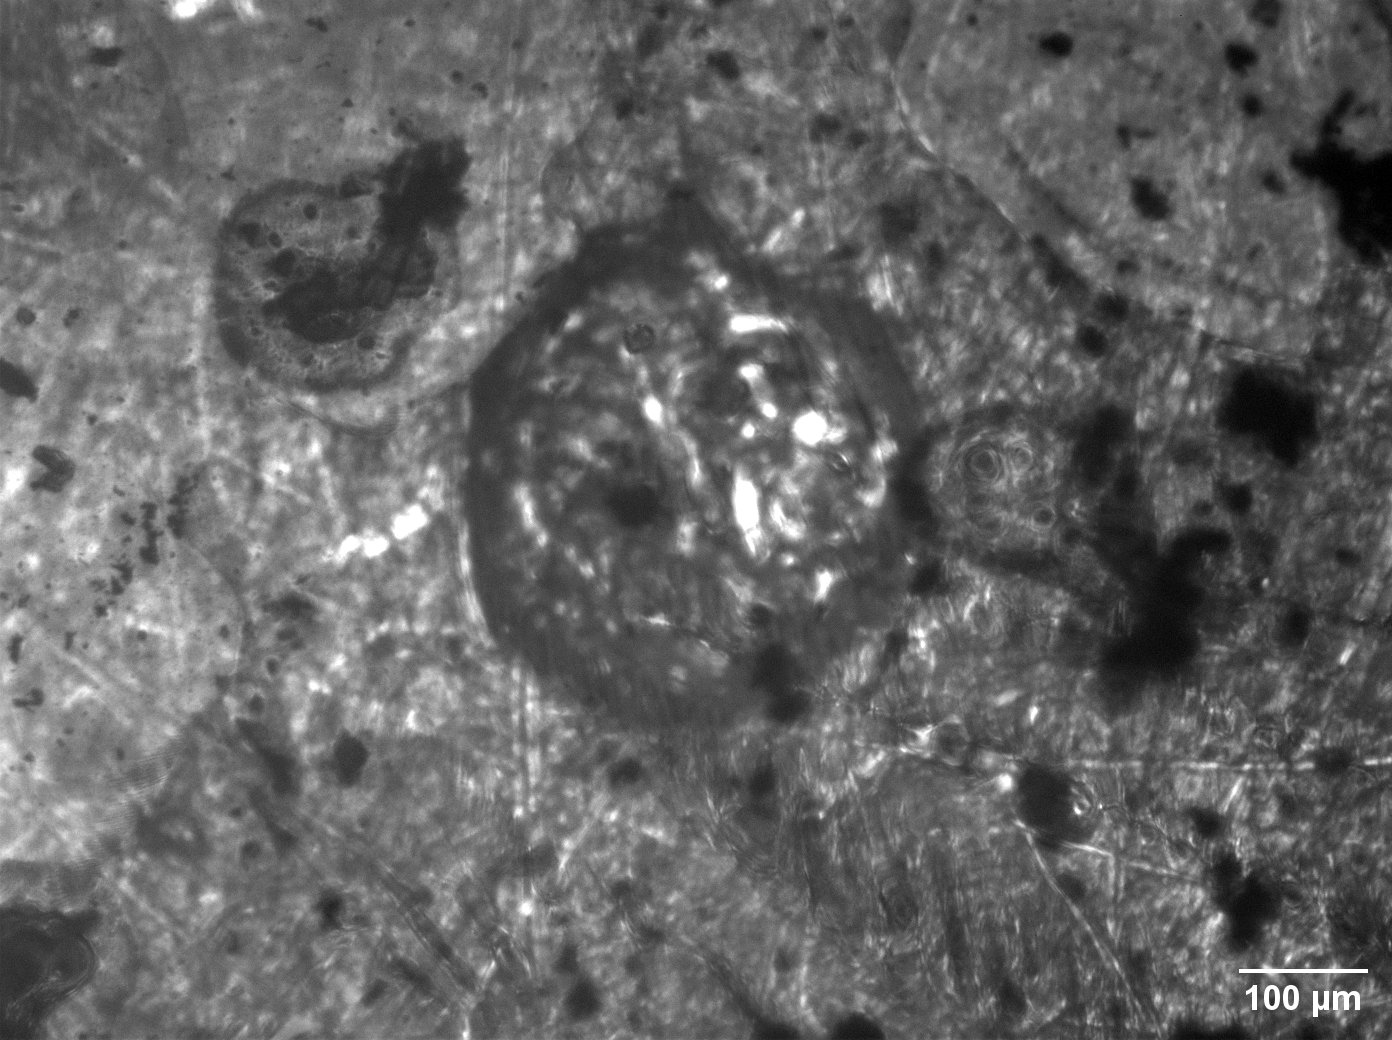
\includegraphics[width=7cm]{4_1_Ice_echtlicht.ome}
		\caption{PDMS 4:1 sample in true light}
	\end{subfigure}
	\begin{subfigure}[]{0.45\textwidth}
		\centering
		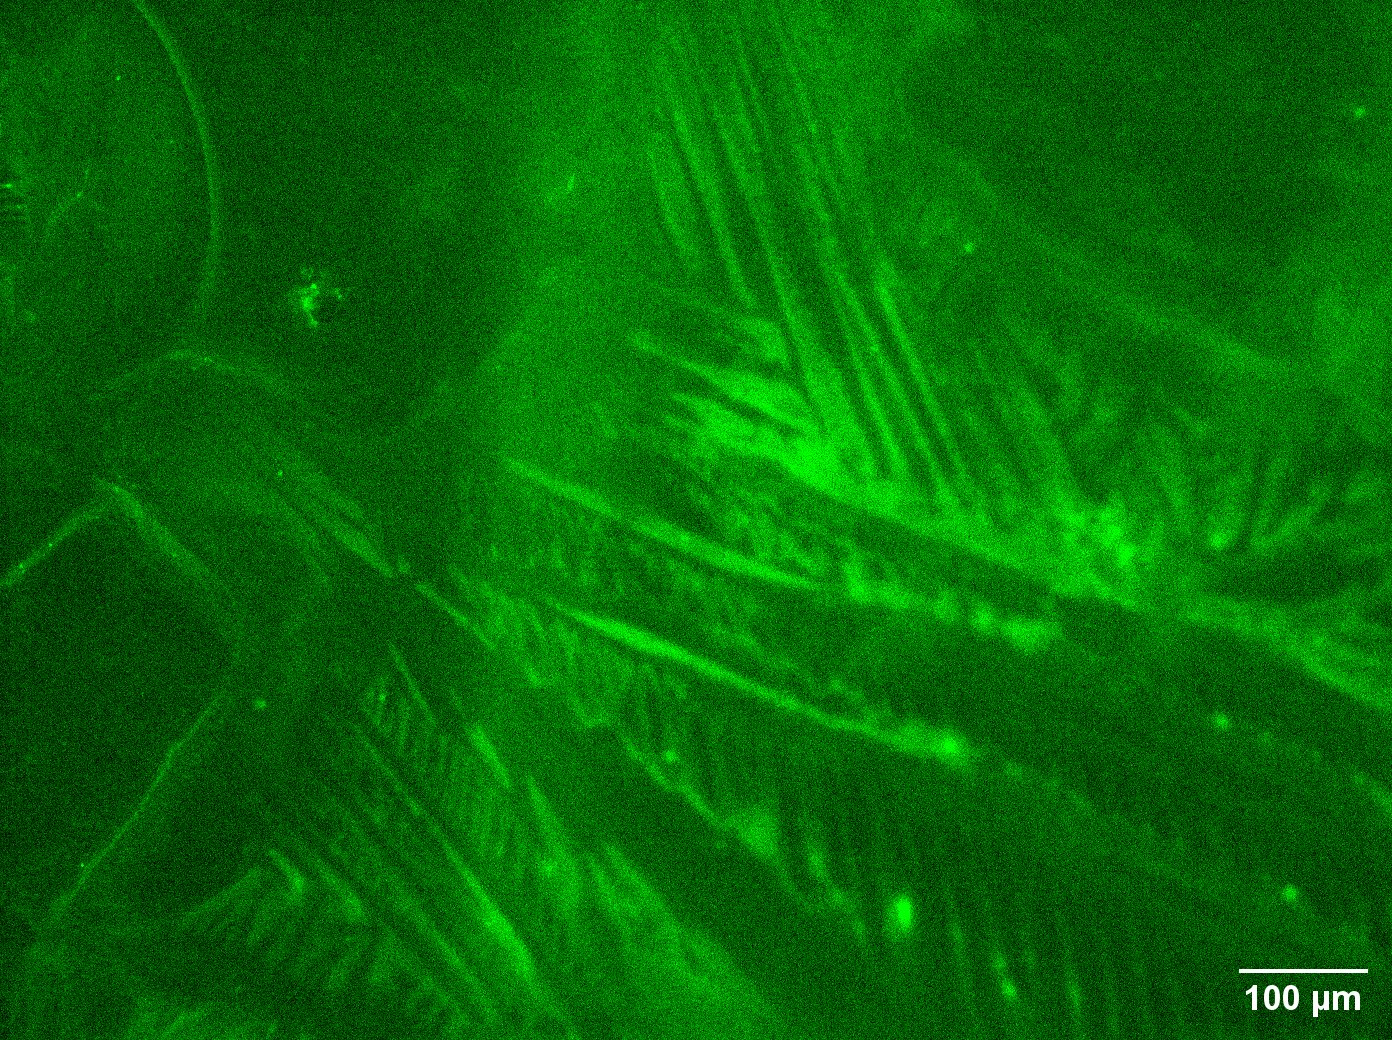
\includegraphics[width=7cm]{4_1_Ice_fluorescence.ome}
		\caption{PDMS 4:1 sample with fluorescence filter}
	\end{subfigure}
	\begin{subfigure}[]{0.45\textwidth}
		\centering
		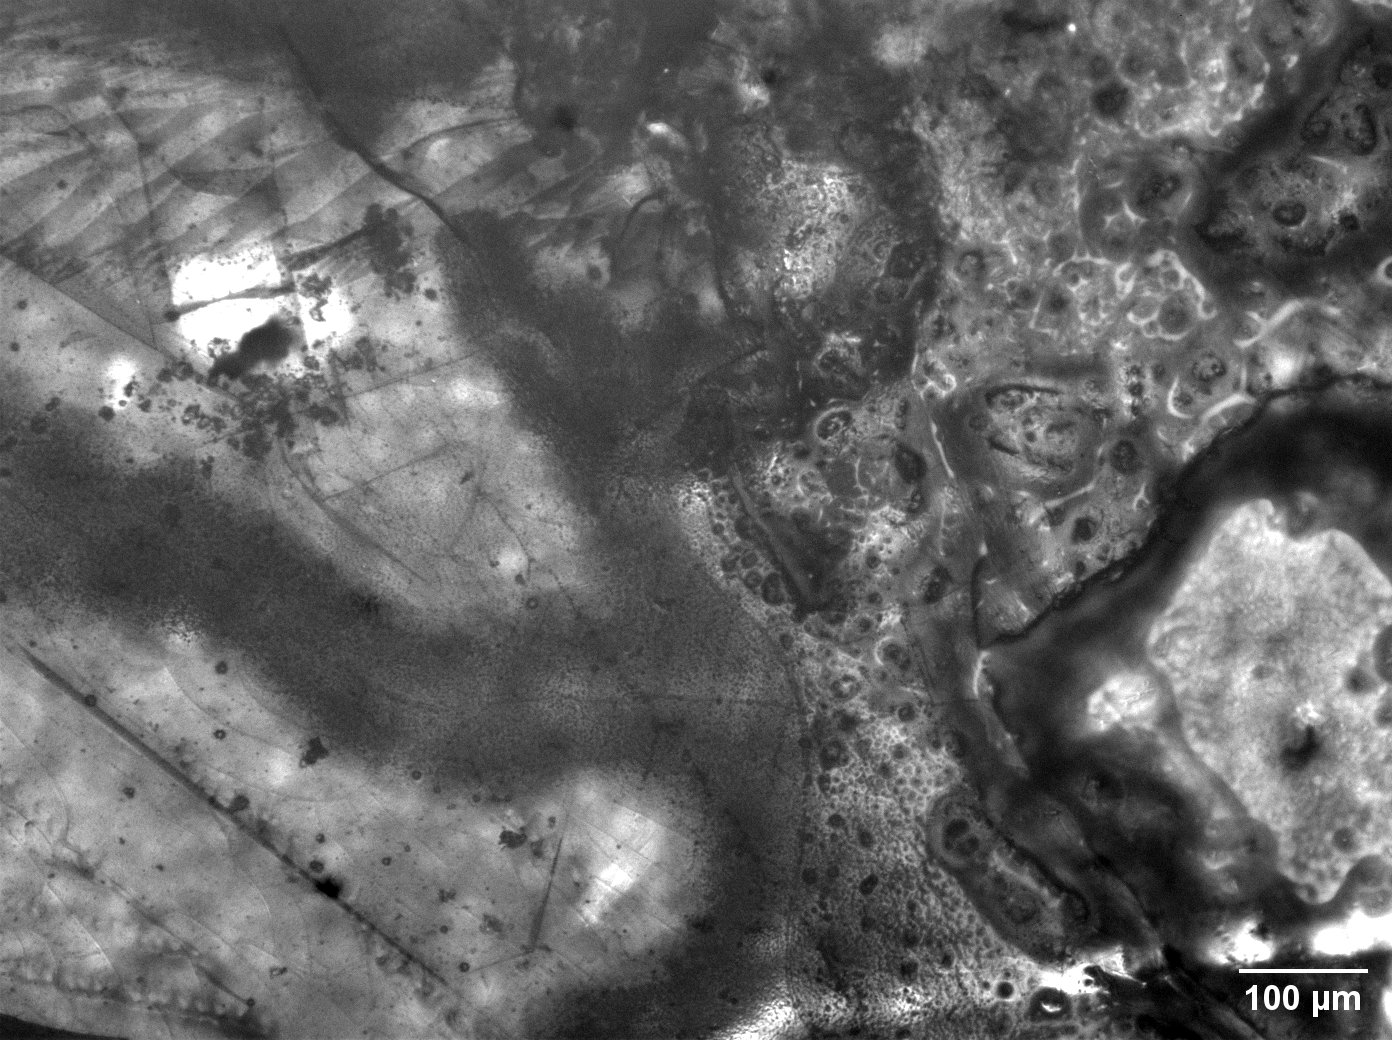
\includegraphics[width=7cm]{50_1_Ice_echtlicht.ome}
		\caption{PDMS 50:1 sample in true light}
	\end{subfigure}
	\begin{subfigure}[]{0.45\textwidth}
		\centering
		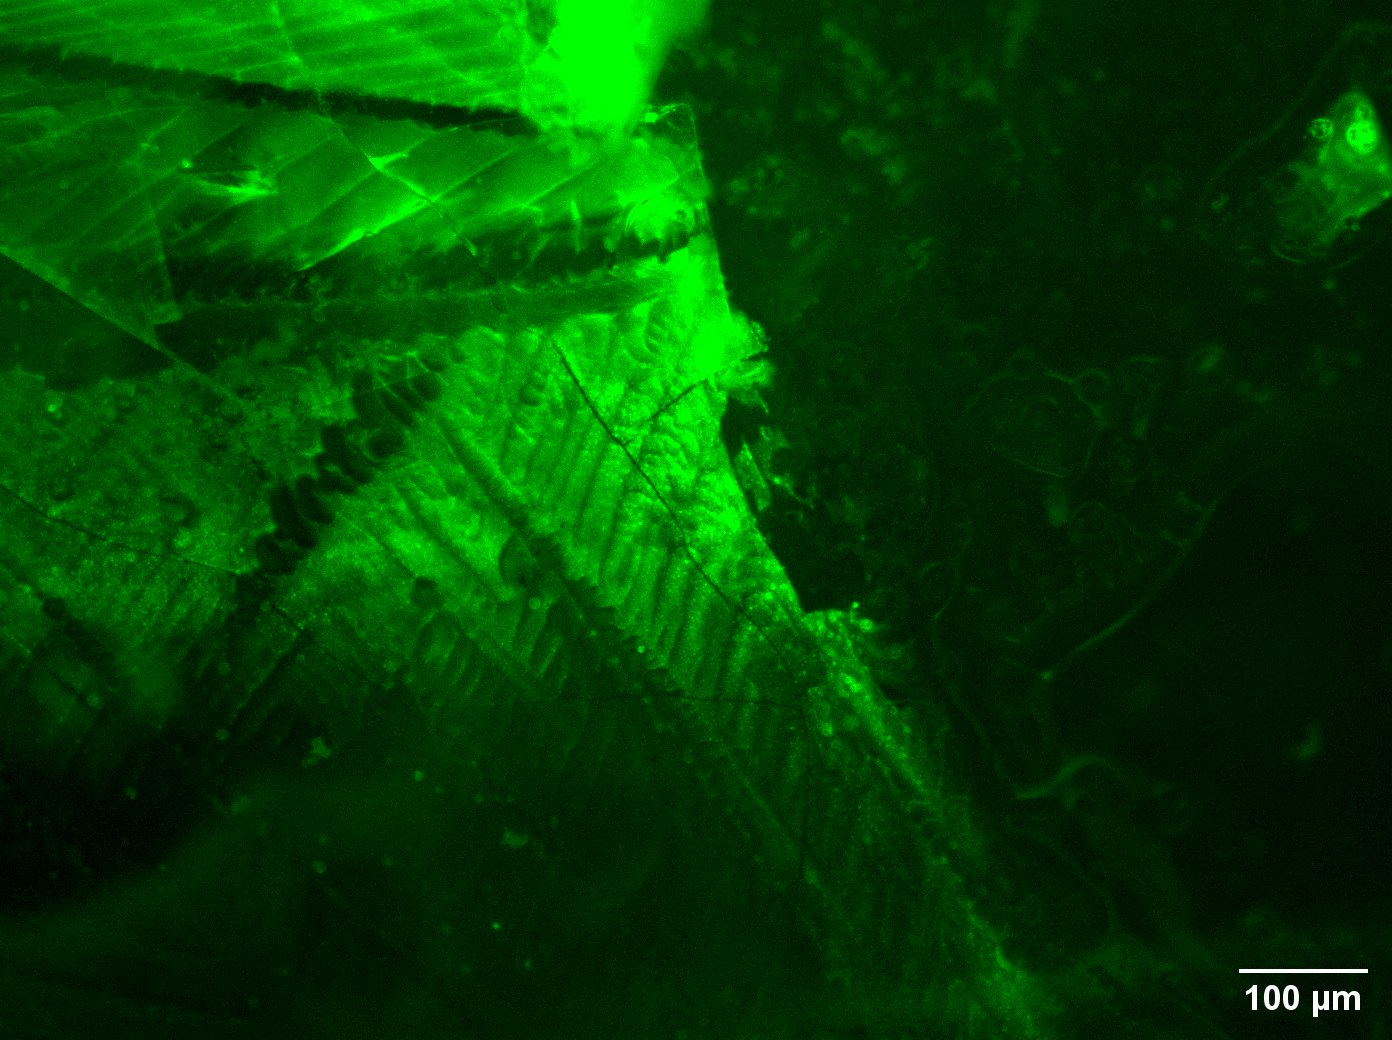
\includegraphics[width=7cm]{50_1_Ice_fluorescence.ome}
		\caption{PDMS 50:1 sample with fluorescence filter}
		\label{fig:VglPDMSicemixtureratio_f}
	\end{subfigure}
	\caption{comparison of ice on different PDMS samples. The ice crystallized ice structure only changes minimally. A continuous ice layer forms over each plasma activated PDMS sample. the layer is only interrupted by the imprint of the pinces at plunge-freezing here visible in (f).}
	\label{fig:VglPDMSicemixtureratio}
\end{figure}

In pulling tests with the finger the three PDMS mixture ratios are tested. For mixture ratio 1:2 and 50:1, all test are unsuccessful (fig. \ref{table:AttemptsPDMS}). however, at mixture ratio 4:1, a successful detachment was performed. However, the detachment cannot be confirmed as the before picture did not cover the area of the missing piece (fig. \ref{fig:SuccessfulDetachment}). without this proof, the formation of the hole when freezing cannot ruled out even if unlikely. Also a piece of ice is not distinguishable when hanging on the finger. Still, since a mixture ratio gave partial succesful results, this mixture ratio needs to be investigated further.

\begin{table}
	\centering
	\begin{tabular}{|c|c|c|c|}
		\hline
		Category & PDMS 1:2 & PDMS 4:1 & PDMS 50:1 \\
		\hline
		\hline
		count executed tries & 5 & 3 & 6\\
		\hline
		unsuccessful & 5 & 2 & 6\\
		\hline
		breaks/movement of ice & 0 & 0 & 0\\
		\hline
		piece lifted with finger & 0 & 1* & 0\\
		\hline		
	\end{tabular}
	\caption{Comparison of detachability between PDMS mixture ratios. Pulling tests at PDMS of 1:2 and 50:1 mixture ratio were unsuccessful. But at mixture ratio of 4:1, detachment was successful one time. However, this could be a statistical outlier or a false positive. A hole was spotted after pulling with the finger. however, the hole is located outside of the before image. therefore the hole could already exist while freezing even if unlikely.}
	\label{table:AttemptsPDMS}
\end{table}

\begin{figure}[hbt!]
	\centering
	\begin{subfigure}[]{0.45\textwidth}
		\centering
		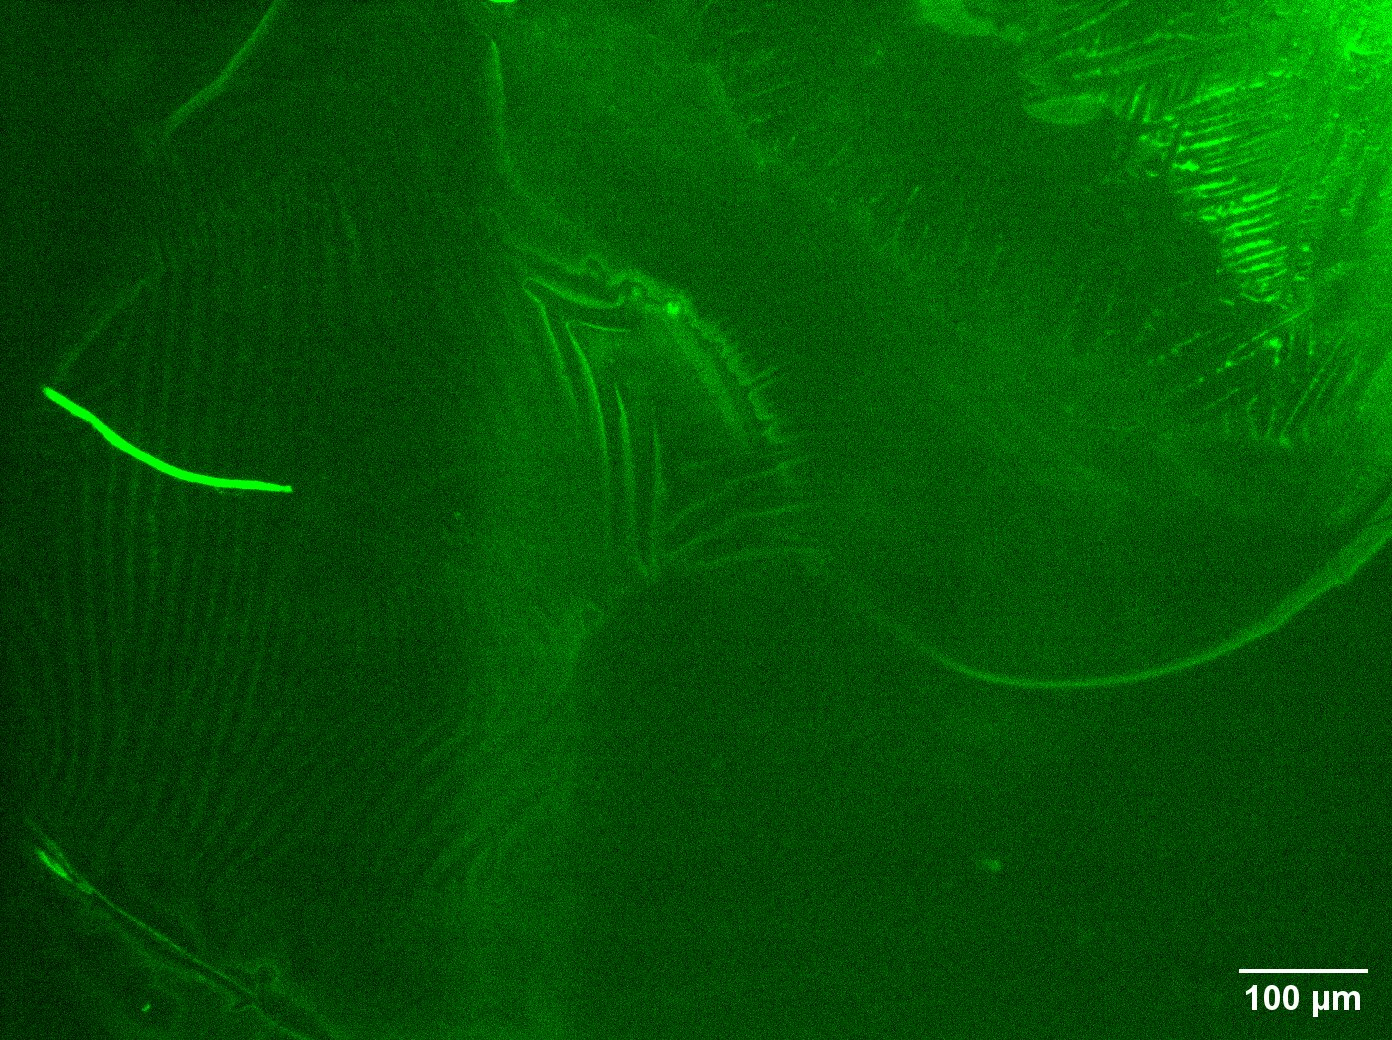
\includegraphics[width=7cm]{Successfu_try_before}
		\caption{Before}
	\end{subfigure}
	\begin{subfigure}[]{0.45\textwidth}
		\centering
		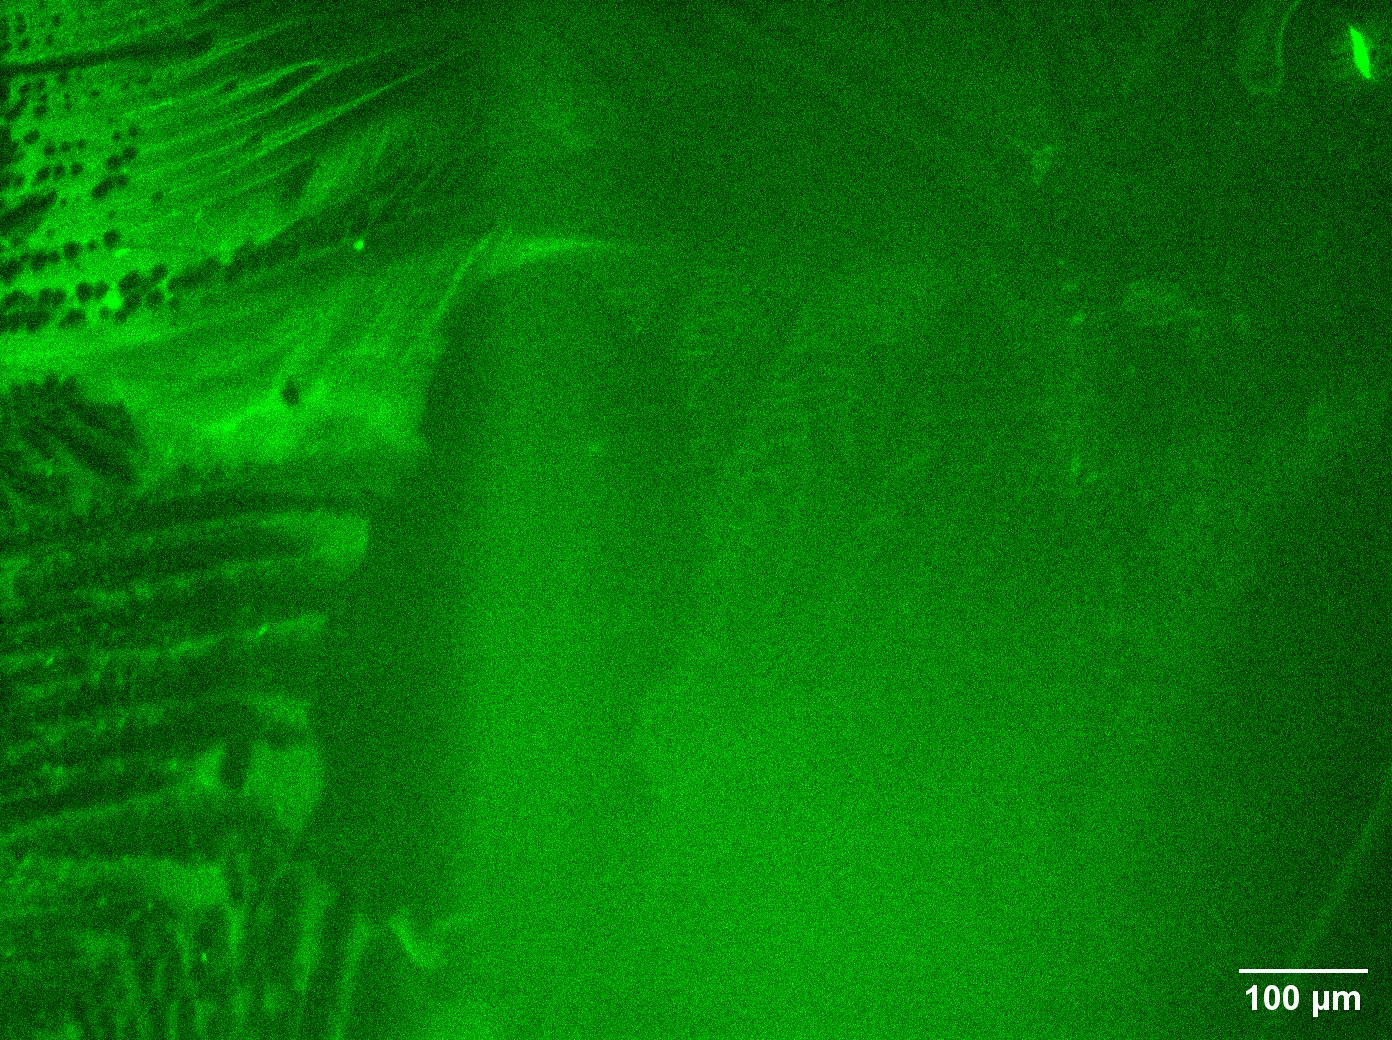
\includegraphics[width=7cm]{Successfu_try_after}
		\caption{After}
	\end{subfigure}
	\caption{Successful pulling test of 4:1 PDMS. However, this result should be taken cautiously. The before and after image each catch a different part of the sample. Under normal circumstances, no holes form in the ice layer when freezing (shown in fig. \ref{fig:VglPDMSicemixtureratio}) however, this case cannot be ruled out.}
	\label{fig:SuccessfulDetachment}
\end{figure}

To test the behavior of an ice layer frozen onto PDMS, the surface is damaged in two ways. In one experiment, the Sample is scratched with a diamond pencil. This is done after mounting the sample on the shuttle. The diamond tip is drawn around the inside of the window several times, forming a visible groove (fig. \ref{fig:ScratchedSample}). In the other experiment, The pincer is intentionally placed through the middle of the sample when plunge-freezing. Therefore an intentional big imprint is left after freezing (fig. \ref{fig:PincerImprint}).

Scratching the ice layer with a diamond pencil 

\begin{figure}[hbt!]
	\centering
	\begin{subfigure}[]{\textwidth}
		\centering
		\begin{subfigure}[]{0.45\textwidth}
			\centering
			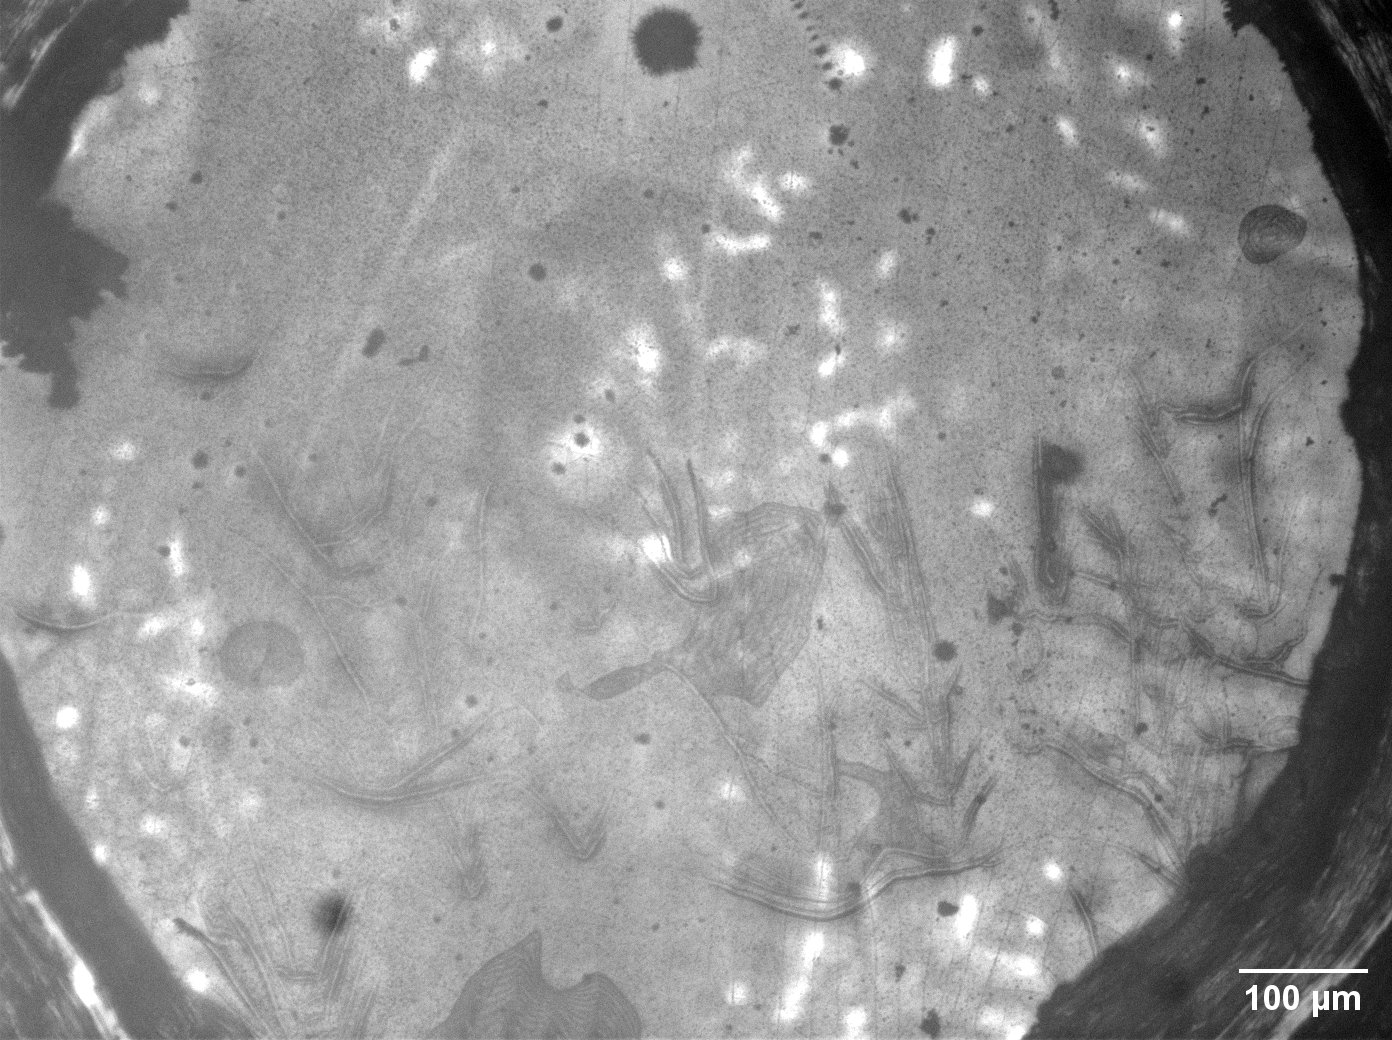
\includegraphics[width=7cm]{SurfaceModDiamontpencil.ome}
		\end{subfigure}	
		\begin{subfigure}[]{0.45\textwidth}
			\centering
			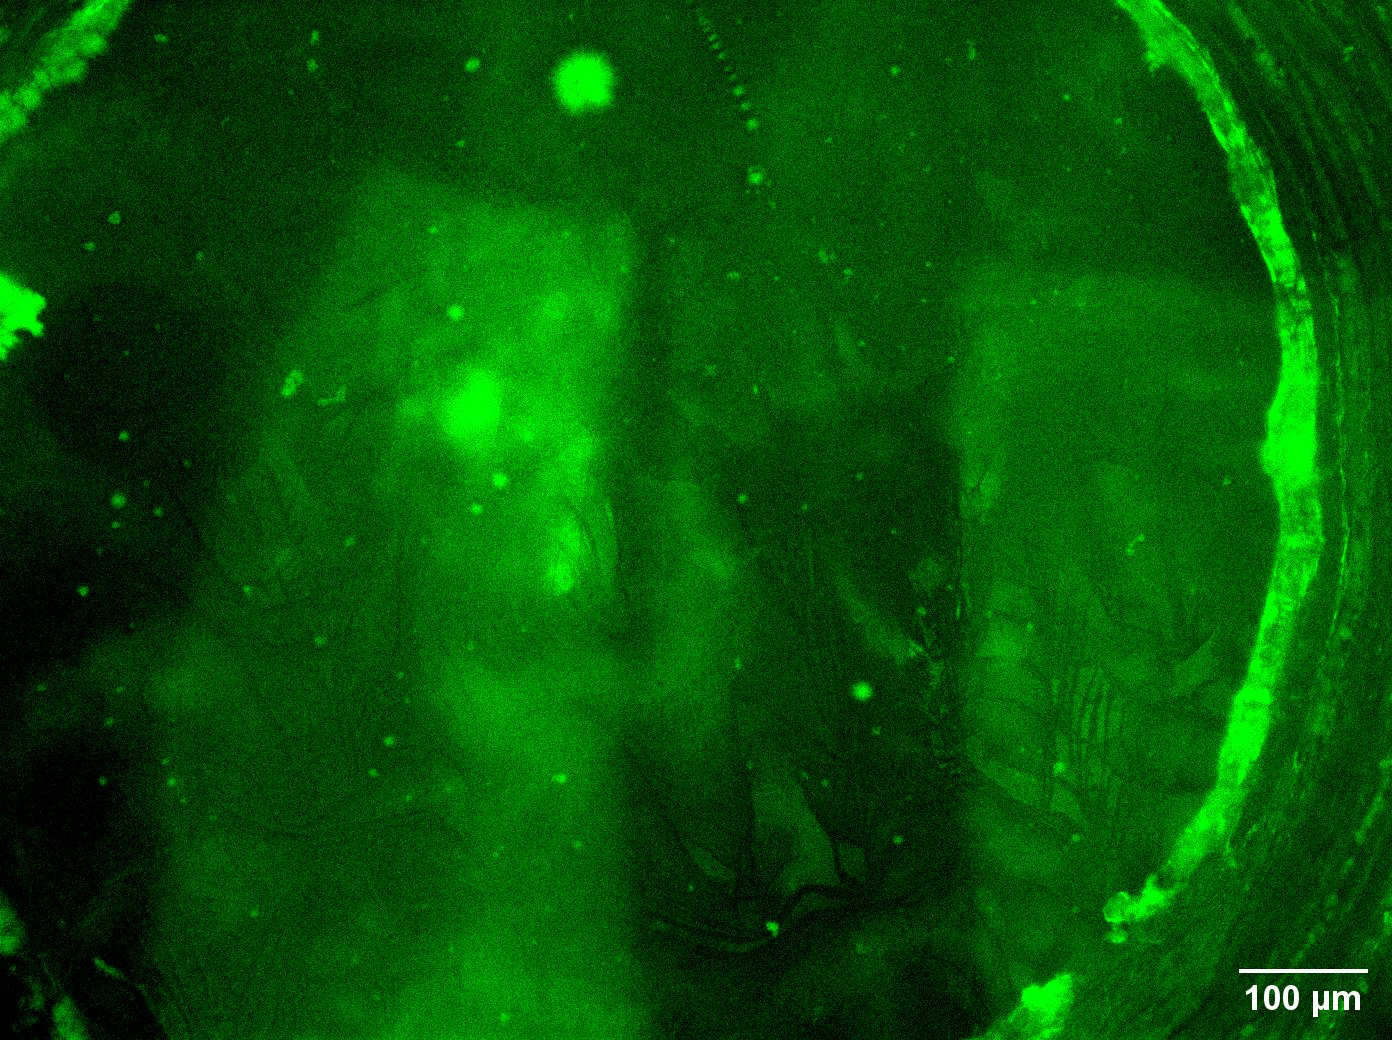
\includegraphics[width=7cm]{SurfaceModDiamontpencilFLuorescence.ome}
		\end{subfigure}
		\caption{Ice layer scratched with diamond pencil.\\}
		\label{fig:ScratchedSample}	
	\end{subfigure}
	\begin{subfigure}[]{\textwidth}
		\centering
		\begin{subfigure}[]{0.45\textwidth}
			\centering		
			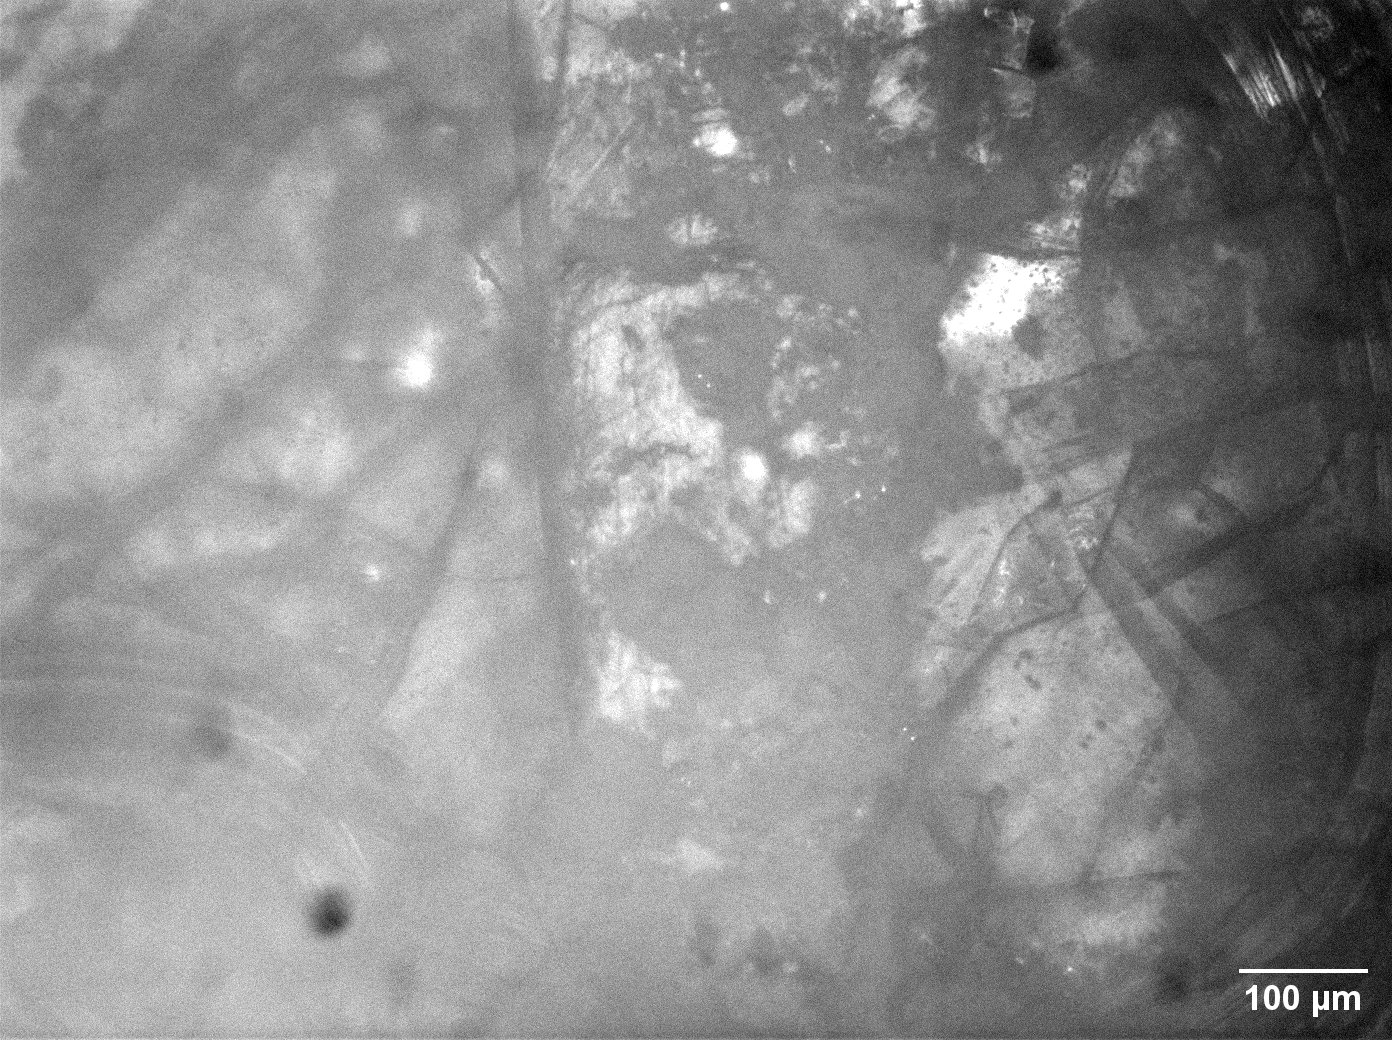
\includegraphics[width=7cm]{SurfaceModPincerReallight.ome}	
		\end{subfigure}
		\begin{subfigure}[]{0.45\textwidth}
			\centering
			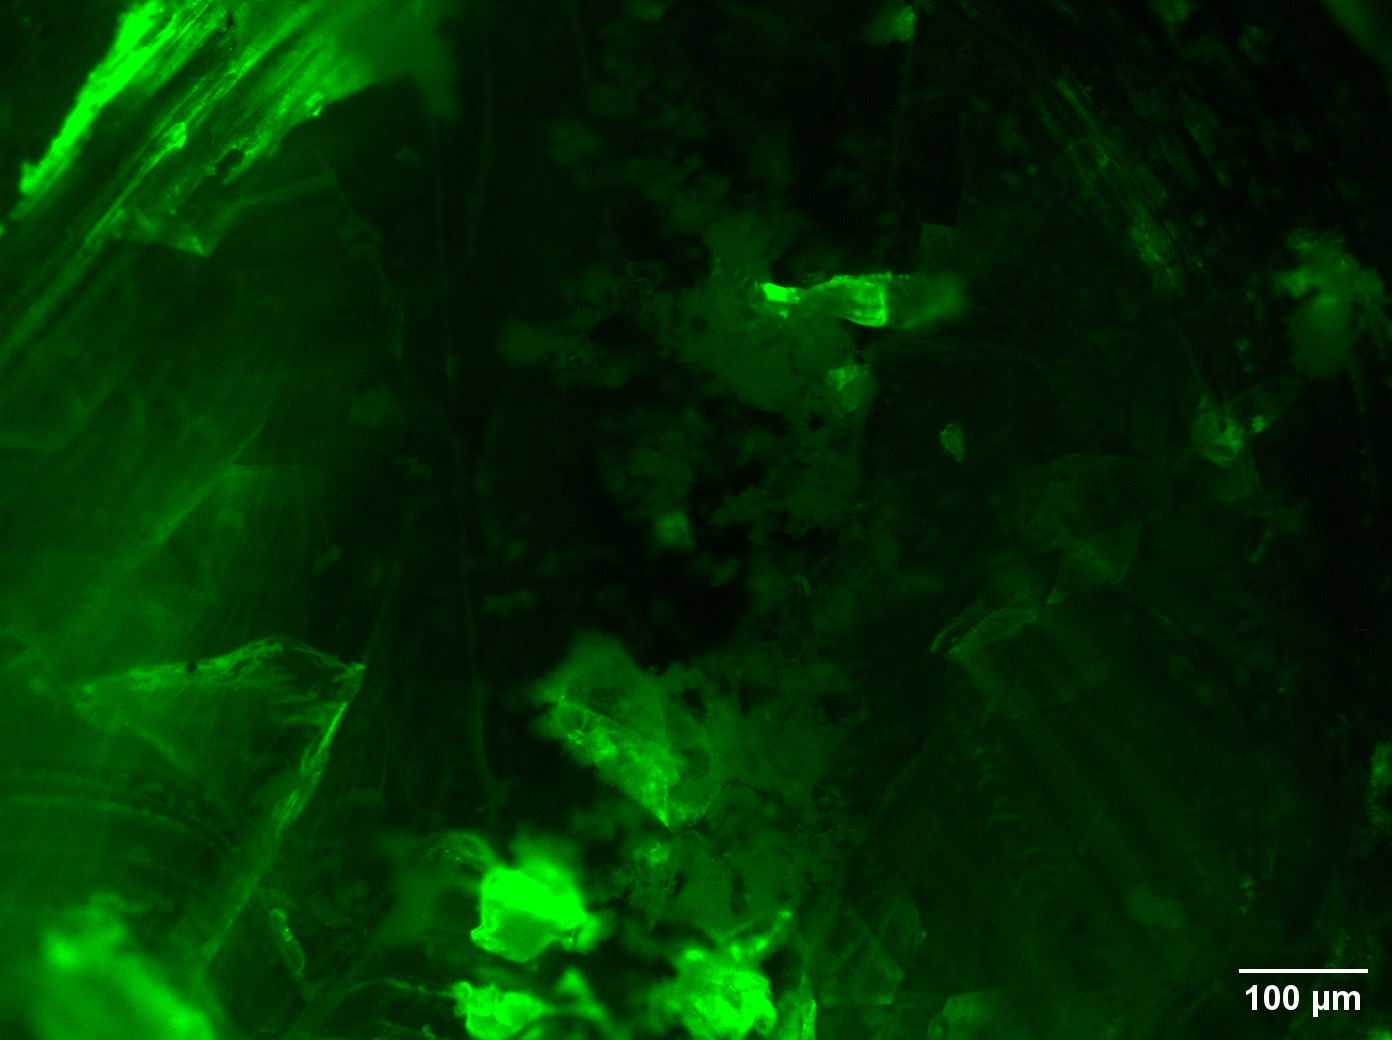
\includegraphics[width=7cm]{SurfaceModPincer.ome}	
		\end{subfigure}
		\caption{Ice layer with loose ice near pincer imprint}
		\label{fig:PincerImprint}
	\end{subfigure}
	\caption{Twod different methods to break the continuos ice surface.}
	\label{fig:SurfaceMod}
\end{figure}

\FloatBarrier



